\providecommand{\toplevelprefix}{../..}  % necessary for subfile bibliography + figures compilation to work, do not move this after documentclass
\documentclass[../../book-main.tex]{subfiles}

\begin{document}

\chapter{Pursuing Low-Dimensional Distributions via Lossy Compression}
\label{ch:compression}\label{ch:general-distribution}

\begin{quote}
	\hfill    ``{\em We compress to learn, and we learn to compress}.''\\
	$~$ \hfill --- High-dimensional Data Analysis, Wright and Ma, 2022
\end{quote}
\vspace{5mm}

In Chapter \ref{ch:linear-independent}, we have shown how to learn simple classes of distributions whose supports are assumed to be either a single or a mixture of low-dimensional subspaces or low-rank Gaussians. For further simplicity, the different (hidden) linear or Gaussian modes are assumed to be orthogonal or independent\footnote{Or can be easily reduced to such idealistic cases.}, as illustrated in Figure \ref{fig:subspaces}. As we have shown, for such special distributions, one can derive rather simple and effective learning algorithms with correctness and efficiency guarantees. The geometric and statistical interpretation of operations in the associated algorithms is also very clear.

In practice, both linearity and independence are rather idealistic assumptions that distributions of real-world high-dimensional data rarely satisfy. The only thing that we may assume is that the intrinsic dimension of the distribution is very low compared to the dimension of the ambient space in which the data are embedded. Hence, in this chapter, we show how to learn a more general class of low-dimensional distributions in a high-dimensional space that is not necessarily (piecewise) linear.

It is typical that the distribution of real data often contains multiple components or modes, say corresponding to different classes of objects in the case of images. These modes might not be statistically independent and they may even have different intrinsic dimensions. It is also typical that we have access to only a finite number of samples of the distribution. Therefore, in  general, we may assume our data are distributed on a mixture of (nonlinear) low-dimensional submanifolds in a high-dimensional space. Figure \ref{fig:mixture-manifolds} illustrates an example of such a distribution.

To learn such a distribution under such conditions, there are several fundamental questions that we need to address:
\begin{itemize}
	\item What is a general approach to learn a general low-dimensional distribution in a high-dimensional space and represent the learned distribution?
	\item How do we measure the complexity of the resulting representation so that we can effectively exploit the low dimensionality to learn?
	\item How do we make the learning process computationally tractable and even scalable, as the ambient dimension is usually high and the number of samples typically large?
\end{itemize}
As we will see, the fundamental idea of {\em compression}, or {\em dimension reduction}, which has been shown to be very effective for the linear/independent case, still serves as a general principle for developing effective computational models and methods for learning general low-dimensional distributions.

Due to its theoretical and practical significance, we will study in greater
depth how this general framework of learning low-dimensional distributions via compression substantiates when the distribution of interest can be well-modeled or approximated by a mixture of low-dimensional subspaces or low-rank Gaussians.
%\yima{I did not touch the above introduction. We can rewrite it when the rest of the chapter is stable. But should state the purpose clearly: a computional framework that strives for achievable and implementable compressive encoding and decoding schemes!}

\begin{figure}
    \centering
    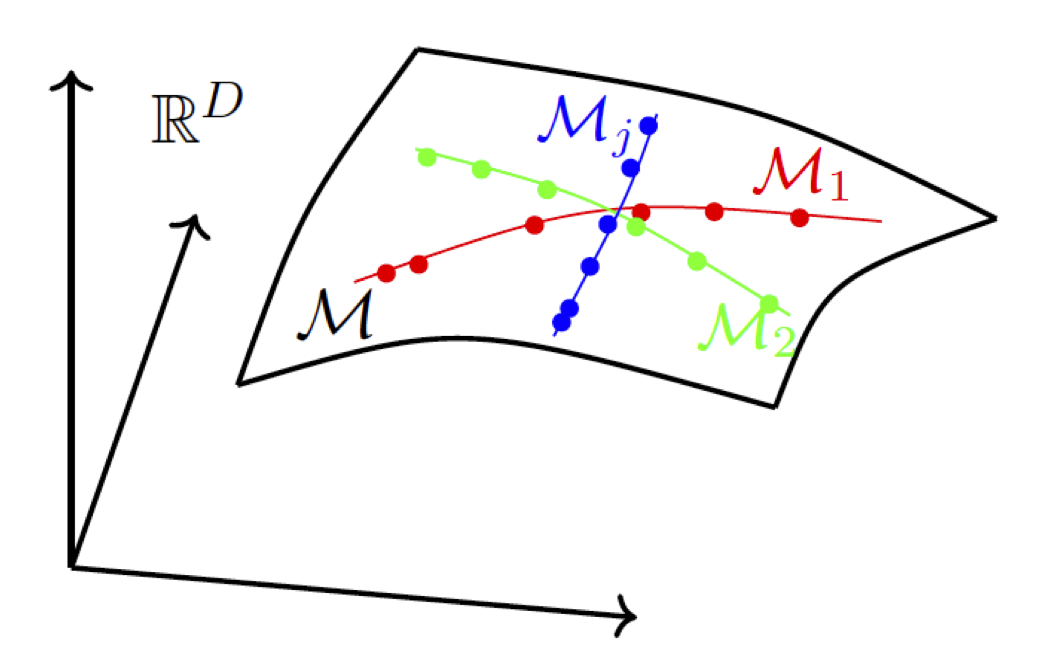
\includegraphics[width=0.5\linewidth]{\toplevelprefix/chapters/chapter3/figs/mixed-manifolds.png}
    \caption{Data distributed on a mixture of low-dimensional submanifolds $\cup_j \mathcal{M}_j$ in a very high-dimensional ambient space, say $\mathbb{R}^D$.}
    \label{fig:mixture-manifolds}
\end{figure}


\section{Entropy Minimization and Compression}

\subsection{Entropy and Coding Rate}
In Chapter \ref{ch:intro}, we have mentioned that the goal of learning is to find the simplest way to generate a given set of data. Conceptually, the Kolmogorov complexity was intended to provide such a measure of complexity but it is not computable and not associated with any implementable scheme that can actually reproduce the data. Hence we need an alternative, computable, and realizable, measure of complexity. That leads us to the notion of {\em entropy}, introduced by Shannon in 1948 \cite{Shannon-1948}.

To illustrate the constructive nature of entropy, let us start with the simplest case. Suppose that we have a discrete random variable that takes $N$ distinct values, or \textit{tokens}, $\{\x_1, \ldots, \x_N\}$ with equal probability $1/N$. Then we could encode each token \(\vx_{i}\) using the \(\log_2 N\)-bit binary representation of \(i\). This coding scheme could be generalized to encoding arbitrary discrete distributions \cite{Cover-Thomas}: Given a distribution \(p\) such that $\sum_{i=1}^N p(\x_i) = 1$, one could assign each token $\x_i$ with probability $p(\x_i)$ to a binary code of size $\log_2 [1/p(\x_i)] = - \log_2 p(\x_i)$ bits. Hence the average number of bits, or {\em the coding rate}, needed to encode any sample from the distribution $p(\cdot)$ is given by the expression:\footnote{By the convention of  Information Theory \cite{Cover-Thomas}, the $\log$ here is to the base $2$. Hence entropy is measured in (binary) bits.}
\begin{equation}
	H(\x) \doteq \mathbb{E}[\log 1/p(\x)]  = - \sum_{i=1}^N p(\x_i) \log  p(\x_i).
	\label{eqn:entropy-discrete}
\end{equation}
This is known as the {\em entropy} of the (discrete) distribution $p(\cdot)$. Note that this entropy is always nonnegative and it is zero if and only if $p(\x_i) = 1$ for some $\x_i$ with $i \in [N]$.\footnote{Here notice that we use the fact $\lim_{p\rightarrow 0} p \log p = 0$.}


\subsection{Differential Entropy}

When the random variable $\x \in \R^{D}$ is continuous and has a probability density $p$, one may view that the limit of the above sum \eqref{eqn:entropy-discrete} is related to an integral:
\begin{equation}
	h(\vx) \doteq \Ex[\log 1/p(\vx)] = - \int_{\R^{D}} p(\vxi) \log p(\vxi) \odif{\vxi}.
	\label{eqn:entropy-differential}
\end{equation}
{More precisely, given a continuous variable $\x$, we may quantize it with a quantization size $\epsilon > 0$. Denote the resulting discrete variable as $\x^\epsilon$. Then one can show that $H(\vx^\epsilon) + \log(\epsilon) \approx h(\vx)$. Hence, when $\epsilon$ is small, the differential entropy $h(\x)$ can be negative. Interested readers may refer to \cite{Cover-Thomas} for a more detailed explanation.}

\begin{example}[Entropy of Gaussian Distributions]
	Through direct calculation, it is possible to show that the entropy of a Gaussian distribution $x \sim \mathcal{N}(\mu, \sigma^2)$ is given by:
	\begin{equation}
		h(x) = \frac{1}{2}\log (2\pi \sigma^2) + \frac{1}{2}.
		\label{eqn:entropy-Gaussian}
	\end{equation}
	It is also known that the Gaussian distribution achieves the maximal entropy
	for all distributions with the same variance $\sigma^2$. The entropy of a multivariate Gaussian distribution $\x \sim \mathcal{N}(\boldsymbol{\mu}, \boldsymbol{\Sigma})$ in $\mathbb{R}^D$ is given by:
	\begin{equation}
		h(\x) = \frac{D}{2}(1 + \log(2\pi)) + \frac{1}{2}\log\det(\boldsymbol{\Sigma}).
		\label{eqn:entropy-Gaussian-multi}
	\end{equation}
\end{example}

Similar to the entropy for a discrete distribution, we would like the
differential entropy to be associated with the coding rate of some realizable
coding scheme. For example, as above, we may discretize the domain of the distribution with a grid of size $\epsilon >0$. The coding rate of the resulting discrete distribution can be viewed as an approximation to the differential entropy \cite{Cover-Thomas}.


Be aware that there are some caveats associated with the definition of
differential entropy. For a distribution in a high-dimensional space, when its
support becomes degenerate (low-dimensional), its differential entropy diverges
to \(-\infty\). This fact is proved in
\Cref{thm:max_entropy} (we also recall the
maximum entropy characterization of the Gaussian distribution mentioned above in
\Cref{thm:max_entropy}) but even in the simple explicit case of Gaussian
distributions \eqref{eqn:entropy-Gaussian-multi}, when the covariance
\(\vSigma\) is singular, we can see that \(\log\det(\vSigma) = -\infty\) so we have $h(\x) = -\infty$. In such a situation, it is not obvious how to properly quantize or encode such a distribution. Nevertheless, degenerate (Gaussian) distributions are precisely the simplest possible, and arguably the most important, instances of low-dimensional distributions in a high-dimensional space. In this chapter, we will discuss a complete resolution to this seeming difficulty with degeneracy.


%\sdb{it seems that it is not so immediate (e.g., the uniform distribution on size-$N$ alphabet has entropy $log_2 N$ bits)... I think the right way to relate them is to consider quantizing the space of values of the continuous r.v.\ $\vx$ into $N$ buckets, calculating discrete entropy for the result, applying a certain correction to the discrete entropy, then taking $N\to\infty$... this correction term seems to be what allows the differential entropy to be negative, whereas the discrete entropy is always nonnegative...}
%\sdb{not sure about this... for example, isn't the Gaussian only ``max entropy'' versus suitably normalized (unit variance) distributions? but my trepidation extends further (by this measure, all perfectly low-dim distributions have $-\infty$ entropy, say)...}




\subsection{Minimizing Coding Rate}\label{sub:min_entropy}
Remember that the learning problem entails the recovery of a (potentially continuous)  distribution $p(\x)$ from a set of samples $\{\x_1, \ldots, \x_N\}$ drawn from the distribution. For ease of exposition, we write $\X = [\x_1, \ldots, \x_N] \in \mathbb{R}^{D\times N}$ . Given that the distributions of interest here are (nearly) low-dimensional, we should expect that their (differential) entropy is very small. But unlike the situations that we have studied in the previous chapter, in general we do not know the family of (analytical) low-dimensional models to which the distribution $p(\x)$ belongs. So checking whether the entropy is small seems to be the only guideline that we can rely on to identify and model the distribution.

Now given the samples alone without knowing what $p(\x)$ is, in theory they could be interpreted as samples from any generic distribution. In particular, they could be interpreted as any of the following cases:
\begin{enumerate}
	\item as samples from the empirical distribution $p^{\vX}$ itself, which assigns $1/N$ probability each of the $N$ samples $\x_i, i=1, \ldots, N$.
	\item as samples from a standard normal distribution $\x^n \sim p^{n} \doteq \mathcal{N}(\boldsymbol{0}, \sigma^2 \boldsymbol{I})$ with a variance $\sigma^2$ large enough (say larger than the sample norms);
	\item as samples from a normal distribution $\x^e \sim p^{e} \doteq \mathcal{N}(\boldsymbol{0}, \hat{\vSigma})$ with a covariance $\hat{\vSigma} = \frac{1}{N} \X \X^T$ being the empirical covariance of the samples;
	\item as samples from a distribution $\hat \x \sim \hat{q}(\vx)$ that closely approximates the ground truth  distribution $p$.
\end{enumerate}
Now the question is which one is better, in what sense? Suppose that you believe these data $\X$ are drawn from a particular distribution  $q(\x)$, which may be one of the above distributions considered. Then we could encode the data points with the optimal code book for the distribution $q(\x)$. The required average coding length (or coding rate) is given by:
\begin{equation}
	\frac{1}{N}\sum_{i=1}^N -\log q(\x_i) \quad \approx \quad - \int_{\R^{D}} p(\vxi) \log q(\vxi)\odif{\vxi}
\end{equation}
as the number of samples $N$ becomes large. If we have identified the correct distribution $p(\x)$, the coding rate is given by the entropy $- \int p(\vxi) \log p(\vxi) \odif{\vxi}$. It turns out that the above coding length $- \int p(\vxi) \log q(\vxi) \odif{\vxi}$ is always larger than or equal to the entropy unless $q(\x) = p(\x)$. Their difference, denoted as
\begin{eqnarray}
	\KL(p \mmid q) &\doteq& - \int_{\R^{D}} p(\vxi) \log q(\vxi) \odif{\vxi}  - \Big(- \int_{\R^{D}} p(\vxi) \log p(\vxi) \odif{\vxi} \Big)\\
	&=& \int_{\R^{D}} p(\vxi) \log \frac{p(\vxi)}{q(\vxi)} \odif{\vxi}
\end{eqnarray}
is known as the {\em Kullback-Leibler} (KL) divergence, or relative entropy. This quantity is always non-negative.
\begin{theorem}[Information Inequality]\label{thm:information-inequality}
	Let $p(\x), q(\x)$ be two probability density functions (that have the same
	support). Then $\KL(p\mmid q) \ge 0$, where the inequality becomes equality if and only if $p = q$.\footnote{Technically, this equality should be taken to mean ``almost everywhere'', i.e., except possibly on a set of zero measure (volume), since this set would not impact the value of any integral.}
\end{theorem}
\begin{proof}
	\begin{eqnarray*}
		- \KL(p\mmid q)
		&=& - \int_{\R^{D}} p(\vxi) \log \frac{p(\vxi)}{q(\vxi)} \odif{\vxi}
		=  \int_{\R^{D}} p(\vxi) \log \frac{q(\vxi)}{p(\vxi)} \odif{\vxi} \\
		&\le& \log \int_{\R^{D}} p(\vxi)  \frac{q(\vxi)}{p(\vxi)} \odif{\vxi} \label{eqn:jensen-KL}
		= \log \int_{\R^{D}} q(\vxi) \odif{\vxi} = \log 1 = 0,
	\end{eqnarray*}
	where the first inequality follows from {\em Jensen's inequality} and the
	fact that the function $\log(\cdot)$ is strictly concave. The equality holds
	if and only if $p = q$ .
\end{proof}

Hence, given a set of sampled data $\X$, to determine which case is better among $p^{n}$, $p^{e}$,  and $\hat{q}$, we may compare their coding rates for $\X$ and see which one gives the lowest rate. We know from the above that the (theoretically achievable) coding rate for a distribution is closely related to its entropy. In general, we have:
\begin{equation}
	h(\x^n) > h(\x^e) > h(\hat \x).
\end{equation}
Hence, if the data $\X$ were encoded by the code book associated with each of these distributions, the coding rate for $\X$ would in general decrease in the same order:
\begin{equation}
	p(\x^n) \rightarrow p(\x^e) \rightarrow p(\hat \x).
\end{equation}

This observation gives us a general guideline on how we may be able to pursue a distribution $p(\x)$ which has a low-dimensional structure. It suggests two possible approaches:
\begin{enumerate}
	\item Starting with a general distribution (say a normal distribution) with high entropy, gradually transforming the distribution towards the (empirical) distribution of the data by reducing entropy.
	\item Among a large family of (parametric or non-parametric) distributions with explicit coding schemes that encode the given data, progressively search for better coding schemes that give lower coding rates.
\end{enumerate}
%\sdb{why not present these through the lens of information gain instead? I think I understand the argument here (a kind of ``coarse to fine'' progression for models of the distribution, with models graded by entropy), but it does not tell us ``when we should stop'' going down this hierarchy of grading. intuitively, it seems like we should ``stop'' when the model is explaining our data well, then the question is how to measure this and how to make it computational...}
Conceptually, both approaches are essentially trying to do the same thing. For the first approach, we need to make sure such a path of transformation exists and is computable. For the second approach, it is necessary that the chosen family is rich enough and can closely approximate (or contain) the ground truth distribution. For either approach, we need to ensure that solutions with lower entropy or better coding rates can be efficiently computed and converge to the desired distribution quickly.\footnote{Say the distribution of real-world data such as images and texts.} We will explore both approaches in the two remaining sections of this chapter.  %\sdb{tension/left unsaid here (from Yi's slides ``elephant in the room''): we cannot actually `know' or in general even efficiently estimate these entropies/divergences in high-dimensional spaces from finite samples (e.g.\ the KL divergence finite sum $\approx$ on the previous page---doesn't this have the curse of dimensionality)... maybe this can be the `hinge' of transition in the next section? (denoising provides a tractable way to perform approximations here), or restructure...}

\section{Compression via Denoising}\label{sub:compression_denoising}

In this section, we will describe a \textit{natural} and \textit{computationally tractable} way to learn a distribution \(p(\vx)\) by way of learning a parametric encoding of our distribution such that the representation has the minimum entropy or coding rate, then using this encoding to transform high-entropy samples from a standard Gaussian into low-entropy samples from the target distribution, as illustrated in \Cref{fig:diffusion-chapter3}. This presents a methodology that utilizes both approaches above in order to learn and sample from the distribution.

\begin{figure}[t]
	\centering
	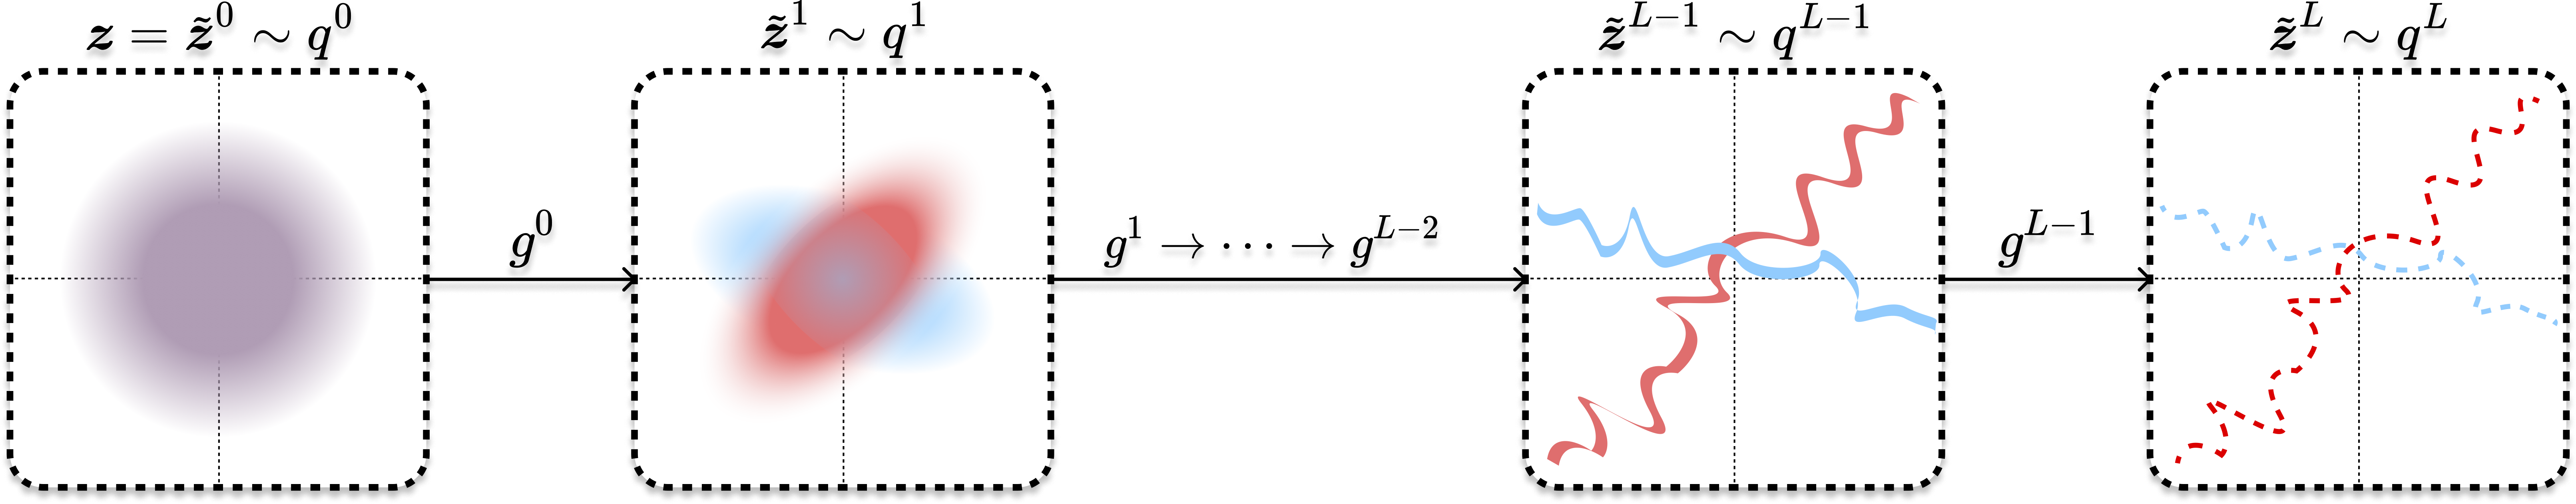
\includegraphics[width=\linewidth]{\toplevelprefix/chapters/chapter3/figs/diffusion_pipeline.png}
	\caption{Illustration of an iterative denoising process that, starting from an isotropic Gaussian distribution, converges to an arbitrary data distribution. }
	\label{fig:diffusion-chapter3}
\end{figure}

\subsection{Diffusion and Denoising Processes} \label{sub:intro_diffusion_denoising}

We first want to find a procedure to decrease the entropy of a given very noisy sample into a lower-entropy sample from the data distribution. Here, we describe a potential approach---one of many, but perhaps the most natural way to attack this problem. First, we find a way to \textit{gradually increase} the entropy of existing samples from the data distribution. Then, we find an \textit{approximate inverse} of this process. But in general, the operation of increasing entropy does not have an inverse, as information from the original distribution may be destroyed. We will thus tackle a special case where (1) the operation of adding entropy takes on a simple, computable, and reversible form; (2) we can obtain a (parametric) encoding of the data distribution, as alluded to in the above pair of approaches. As we will see, the above two factors will ensure that our approach is possible.

We will increase the entropy in arguably the simplest possible way, i.e., \textit{adding isotropic Gaussian noise}. More precisely, given the random variable \(\vx\), we can consider the \textit{stochastic process} \((\vx_{t})_{t \in [0, T]}\) which adds gradual noise to it, i.e.,
\begin{equation}\label{eq:additive_gaussian_noise_model}
	\vx_{t} \doteq \vx + t\vg, \qquad \forall t \in [0, T],
\end{equation}
where \(T \in [0, \infty]\) is a time horizon and \(\vg \sim \dNorm(\vzero, \vI)\) is drawn independently of \(\vx\). This process is an example of a \textit{diffusion process}, so-named because it spreads out the probability mass out over all of \(\R^{D}\) as time goes on, increasing the entropy over time. This intuition is confirmed graphically by \Cref{fig:ve_forward_density}, and rigorously via the following theorem.
\begin{theorem}[Simplified Version of \Cref{thm:diffusion_entropy_increases}]
	Suppose that \((\vx_{t})_{t \in [0, T]}\) follows the model \eqref{eq:additive_gaussian_noise_model}. For any \(t \in (0, T]\), the random variable \(\vx_{t}\) has differential entropy \(h(\vx_{t}) > -\infty\). Moreover, under certain technical conditions on \(\vx\), 
	\begin{equation}
		\odv*{h(\vx_{t})}{t} > 0, \qquad \forall t \in (0, T],
	\end{equation}
	showing that the entropy of the noised \(\vx\) increases over time \(t\).
\end{theorem}
The proof is elementary, but it is rather long, so we postpone it to \Cref{sub:diffusion_entropy_increases}. The main as-yet unstated implication of this result is that \(h(\vx_{t}) > h(\vx)\) for every \(t > 0\). To see this, note that if \(h(\vx) = -\infty\) then \(h(\vx_{t}) > -\infty\) for all \(t > 0\),  and if \(h(\vx) > -\infty\) then \(h(\vx_{t}) = h(\vx) + \int_{0}^{t}[\odv*{h(\vx_{s})}{s}]\odif{s} > h(\vx)\) by the fundamental theorem of calculus, so in both cases \(h(\vx_{t}) > h(\vx)\) for every \(t > 0\).

\begin{figure}
	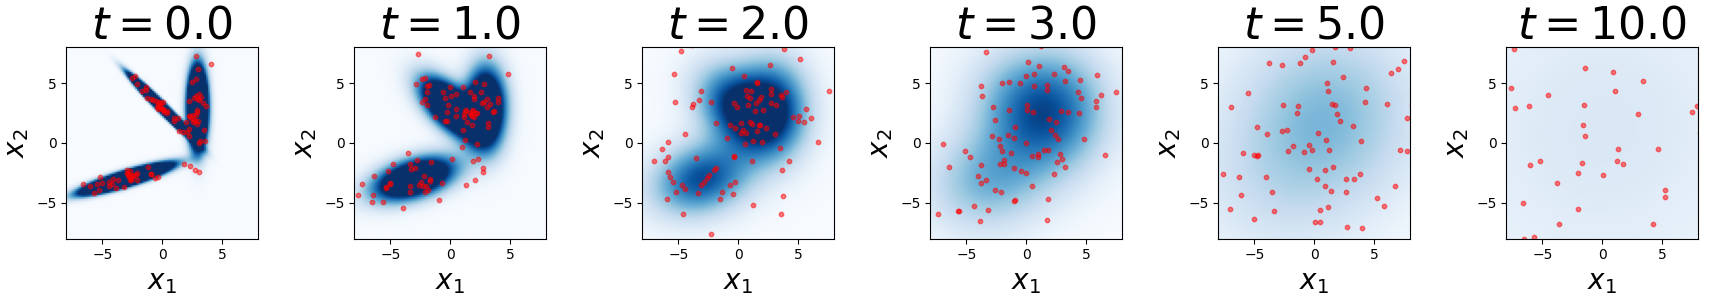
\includegraphics[width=\textwidth]{\toplevelprefix/chapters/chapter3/figs/ve_forward_diffusion_density.png}
	\caption{\small\textbf{Diffusing a mixture of Gaussians.} From left to right, we observe the evolution of the density as \(t\) grows from \(0\) to \(10\), along with some representative samples. Each region is colored by its density (\(0.0\) is completely white, \(> 0.01\) is very dark blue, every other value maps to some shade of blue in between.) We observe that the probability mass gets less concentrated as \(t\) increases, signaling that entropy increases.}
	\label{fig:ve_forward_density}
\end{figure}

The inverse operation to adding noise is known as \textit{denoising}. It is a classical and well-studied topic in signal processing and system theory, such as the Wiener filter and the Kalman filter. The several problems discussed in \Cref{ch:classic}, such as PCA, ICA, and Dictionary Learning, are specific instances of the denoising problem. For a fixed \(t\) and the additive Gaussian noise model \eqref{eq:additive_gaussian_noise_model}, the denoising problem can be formulated as attempting to learn a function \(\bar{\vx}^{\ast}(t, \cdot)\) which forms the best possible approximation (in expectation) of the true random variable \(\vx\), given both \(t\) and \(\vx_{t}\):
\begin{equation}\label{eq:denoising_loss}
	\bar{\vx}^{\ast}(t, \cdot) \in \argmin_{\bar{\vx}(t, \cdot)}\Ex_{\vx, \vx_{t}}\norm{\vx - \bar{\vx}(t, \vx_{t})}_{2}^{2}.
\end{equation}
The solution to this problem, when optimizing \(\bar{\vx}(t, \cdot)\) over all possible (square-integrable) functions, is the so-called \textit{Bayes optimal denoiser}: 
\begin{equation}\label{eq:optimal_denoiser}
	\bar{\vx}^{\ast}(t, \vxi) \doteq \Ex[\vx \mid \vx_{t} = \vxi].
\end{equation}

This expression justifies the notation \(\bar{\vx}\), which is meant to compute a conditional expectation (i.e., conditional mean or conditional average). In short, it attempts to remove the noise from the noisy input, outputting the best possible guess (in expectation and w.r.t.~the \(\ell^{2}\)-distance) of the (de-noised) original random variable.

\begin{example}[Denoising Gaussian Noise from a Mixture of Gaussians]\label{example:denoising_gaussian_mixture}
	In this example we compute the Bayes optimal denoiser for an incredibly important class of distributions, the Gaussian mixture model. To start, let us fix parameters for the distribution: mixture weights \(\vpi \in \R^{K}\), component means \(\{\vmu_{k}\}_{k = 1}^{K} \subseteq \R^{D}\), and component covariances \(\{\vSigma_{k}\}_{k = 1}^{K} \subseteq \PSD(D)\), where  \(\PSD(D)\) is the set of \(D \times D\) symmetric positive semidefinite matrices. Now, suppose \(\vx\) is generated by the following two-step procedure:
	\begin{itemize}
		\item First, an index (or \textit{label}) \(y \in [K]\) is sampled such that \(y = k\) with probability \(\pi_{k}\).
		\item Second, \(\vx\) is sampled from the normal distribution \(\dNorm(\vmu_{y}, \vSigma_{y})\).
	\end{itemize}
	Then \(\vx\) has distribution
	\begin{equation}
		\vx \sim \sum_{k = 1}^{K}\pi_{k}\dNorm(\vmu_{k}, \vSigma_{k}),
	\end{equation}
	and so 
	\begin{equation}
		\vx_{t} = \vx + t\vg \sim \sum_{k = 1}^{K}\pi_{k}\dNorm(\vmu_{k}, \vSigma_{k} + t^{2}\vI).
	\end{equation}
	Let us define \(\phi(\vx ; \vmu, \vSigma)\) as the probability density of \(\dNorm(\vmu, \vSigma)\) evaluated at \(\vx\). In this notation, the density of \(\vx_{t}\) is 
	\begin{equation}
		p_{t}(\vx_{t}) = \sum_{k = 1}^{K}\pi_{k}\phi(\vx_{t} ; \vmu_{k}, \vSigma_{k} + t^{2}\vI).
	\end{equation}

	Conditioned on \(y\), the variables are jointly Gaussian: if we say that \(\vx = \vmu_{y} + \vSigma_{y}^{1/2}\vu\) where \((\cdot)^{1/2}\) is the matrix square root and \(\vu \sim \dNorm(\vzero, \vI)\) independently of \(y\) (and \(\vg\)), then we have
	\begin{equation}
		\mat{\vx \\ \vx_{t}} = \mat{\vmu_{y} \\ \vmu_{y}} + \mat{\vSigma_{y}^{1/2} & \vzero \\ \vSigma_{y}^{1/2} & t\vI}\mat{\vu \\ \vg}.
	\end{equation}
	This shows that \(\vx\) and \(\vx_{t}\) are jointly Gaussian (conditioned on \(y\)) as claimed. Thus we can write
	\begin{equation}
		\mat{\vx \\ \vx_{t}} \sim \dNorm\rp{\mat{\vmu_{y} \\ \vmu_{y}}, \mat{\vSigma_{y} & \vSigma_{y} \\ \vSigma_{y} & \vSigma_{y} + t^{2}\vI}}.
	\end{equation}
	Thus the conditional expectation of \(\vx\) given \(\vx_{t}\) (i.e., the
	Bayes optimal denoiser conditioned on \(y\)) is famously
	(\Cref{exercise:conditional_gaussian})
	\begin{equation}
		\Ex[\vx \mid \vx_{t}, y] = \vmu_{y} + \vSigma_{y}(\vSigma_{y} + t^{2}\vI)^{-1}(\vx_{t} - \vmu_{y}).
	\end{equation}
	To find the overall Bayes optimal denoiser, we use the law of iterated expectation, obtaining
	\begin{align}
		\bar{\vx}^{\ast}(t, \vx_{t})
		&= \Ex[\vx \mid \vx_{t}] \\ 
		&= \Ex[\Ex[\vx \mid \vx_{t}, y] \mid \vx_{t}] \\ 
		&= \sum_{k = 1}^{K}\Pr[y = k \mid \vx_{t}]\Ex[\vx \mid \vx_{t}, y = k].
	\end{align}
	The probability can be dealt with as follows. Let \(p_{t \mid y}\) be the probability density of \(\vx_{t}\) conditioned on the value of \(y\). Then
	\begin{align}
		\Pr[y = k \mid \vx_{t}]
		&= \frac{p_{t \mid y}(\vx_{t} \mid k)\pi_{k}}{p_{t}(\vx_{t})} \\ 
		&= \frac{\pi_{k}\phi(\vx_{t} ; \vmu_{k}, \vSigma_{k}
		+ t^{2}\vI)}{\sum_{i = 1}^{K}\pi_{i}\phi(\vx_{t} ; \vmu_{i}, \vSigma_{i} + t^{2}\vI)}.
	\end{align}
	On the other hand, the conditional expectation is as described before:
	\begin{equation}
		\Ex[\vx \mid \vx_{t}, y = k] = \vmu_{k} + \vSigma_{k}(\vSigma_{k} + t^{2}\vI)^{-1}(\vx_{t} - \vmu_{k}).
	\end{equation}
	So putting this all together, the true Bayes optimal denoiser is 
	\begin{equation}\label{eq:gmm_bayes_optimal_denoiser}
		\bar{\vx}^{\ast}(t, \vx_{t}) = \sum_{k = 1}^{K}\frac{\pi_{k}\phi(\vx_{t}
		;\vmu_{k}, \vSigma_{k} + t^{2}\vI)}{\sum_{i = 1}^{K}\pi_{i}\phi(\vx_{t}
		;\vmu_{i}, \vSigma_{i} + t^{2}\vI)}\cdot\bp{\vmu_{k} + \vSigma_{k}(\vSigma_{k} + t^{2}\vI)^{-1}(\vx_{t} - \vmu_{k})}.
	\end{equation}
	This example is particularly important, and several special cases will give us great conceptual insight later. For now, let us attempt to extract some geometric intuition from the functional form of the optimal denoiser \eqref{eq:gmm_bayes_optimal_denoiser}.

	To try to understand \eqref{eq:gmm_bayes_optimal_denoiser} intuitively, let us first set \(K = 1\) (i.e., one Gaussian) such that \(\vx \sim \dNorm(\vmu, \vSigma)\). Let us then diagonalize \(\vSigma = \vV\vLambda \vV^{\top}\). Then the Bayes optimal denoiser is 
	\begin{equation}
		\bar{\vx}^{\ast}(t, \vx_{t}) = \vmu + \vSigma(\vSigma + t^{2}\vI)^{-1}(\vx_{t} - \vmu) = \vmu + \vV\mat{\lambda_{1}/(\lambda_{1} + t^{2}) & & \\ & \ddots & \\ & & \lambda_{D}/(\lambda_{D} + t^{2})}\vV^{\top}(\vx_{t} - \vmu),
	\end{equation}
	where \(\lambda_{1}, \dots, \lambda_{D}\) are the eigenvalues of \(\vSigma\). We can observe that this denoiser has three steps:
	\begin{itemize}
		\item Translate the input \(\vx_{t}\) by \(\vmu\).
		\item Contract the (translated) input \(\vx_{t} - \vmu\) in each eigenvector direction by a quantity \(\lambda_{i}/(\lambda_{i} + t^{2})\). If the translated input is low-rank and some eigenvalues of \(\vSigma\) are zero, these directions get immediately contracted to \(0\) by the denoiser, ensuring that the output of the contraction is similarly low-rank.
		\item Translate the output back by \(\vmu\).
	\end{itemize}
	It is easy to show that it contracts the current \(\vx_{t}\) towards the mean \(\vmu\):
	\begin{equation}\label{eq:contraction}
		\norm{\bar{\vx}^{\ast}(t, \vx_{t}) - \vmu}_{2} \leq \norm{\vx_{t} - \vmu}_{2}.
	\end{equation}

	This is the geometric interpretation of the denoiser of a \textit{single} Gaussian. The overall denoiser of the Gaussian mixture model \eqref{eq:gmm_bayes_optimal_denoiser} uses \(K\) such denoisers, weighting their output by the posterior probabilities \(\Pr[y = k \mid \vx_{t}]\). If the means of the Gaussians are well-separated, these posterior probabilities are very close to \(0\) or \(1\) near each mean or cluster. In this regime, the overall denoiser \eqref{eq:gmm_bayes_optimal_denoiser} has the same geometric interpretation as the above single Gaussian denoiser.

    At first glance, such a contraction mapping \eqref{eq:contraction} may appear similar to power iterations (see \Cref{subsec:power iterations}).  However, the two are fundamentally different. Power iteration implements a contraction mapping towards a subspace---namely the subspace spanned by the first principal component. In contrast, the iterates in \eqref{eq:contraction} converge to the mean \(\vmu\) of the underlying distribution, which is a single point.  
\end{example}

\begin{figure}
	\centering 
	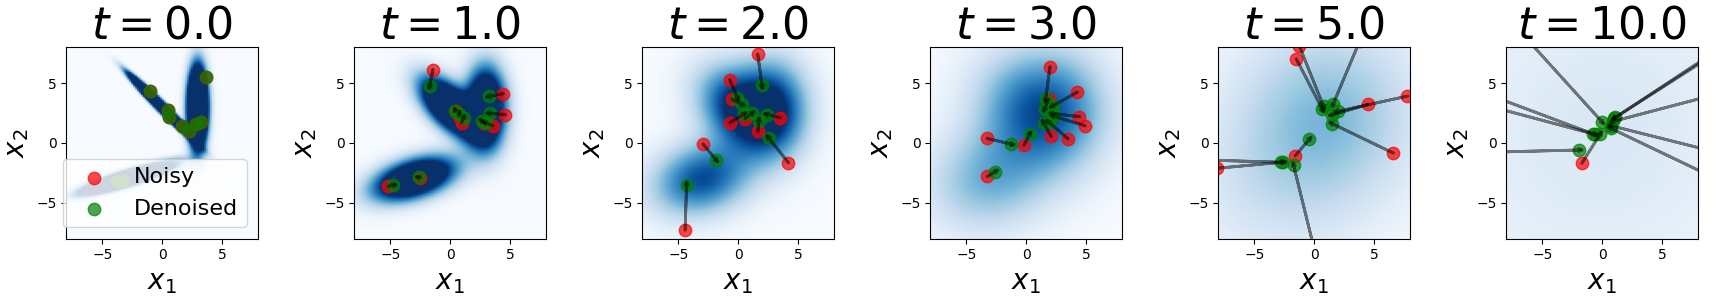
\includegraphics[width=\textwidth]{\toplevelprefix/chapters/chapter3/figs/ve_forward_diffusion_denoising.png}\vspace{-0.15in}
	\caption{\small \textbf{Bayes optimal denoiser and score of a Gaussian mixture model.} In the same setting as \Cref{fig:ve_forward_density}, we demonstrate the effect of the Bayes optimal denoiser \(\bar{\vx}^{\ast}\) by plotting \(\vx_{t}\) (red) and \(\bar{\vx}^{\ast}(t, \vx_{t})\) (green) for some choice \(t\) and \(\vx_{t}\). By Tweedie's formula \Cref{thm:tweedie}, the residual between them is proportional to the so-called (Hyv\"arinen) score \(\nabla_{\vx_{t}}\log p_{t}(\vx_{t})\). We can see that the score points towards the modes of the distribution of \(\vx_{t}\).}
	\label{fig:ve_forward_denoising}
\end{figure}

Intuitively, and as we can see from \Cref{example:denoising_gaussian_mixture}, the Bayes optimal denoiser \(\bar{\vx}^{\ast}(t, \cdot)\) should move its input \(\vx_{t}\) towards the modes of the distribution of \(\vx\). It turns out that, actually, we can quantify this by showing that the Bayes optimal denoiser \textit{takes a gradient ascent step} on the (log-)density of \(\vx_{t}\), which (recall) we denoted \(p_{t}\). That is, following the denoiser means moving from the input iterate to a region of higher probability within this (perturbed) distribution. For small \(t\), the perturbation is small so our initial intutition is therefore (almost) exactly right. The picture is visualized in \Cref{fig:ve_forward_denoising} and rigorously formulated as Tweedie's formula \cite{Robbins1956AnEB}.
\begin{theorem}[Tweedie's Formula]\label{thm:tweedie}
	Suppose that \((\vx_{t})_{t \in [0, T]}\) obeys \eqref{eq:additive_gaussian_noise_model}. Let \(p_{t}\) be the density of \(\vx_{t}\) (as previously declared). Then 
	\begin{equation}\label{eq:tweedie}
		\Ex[\vx \mid \vx_{t}] = \vx_{t} + t^{2}\nabla_{\vx_{t}} \log p_{t}(\vx_{t}).
	\end{equation}
\end{theorem}
\begin{proof}
	For the proof let us suppose that \(\vx\) has a density (even though the
	theorem is true without this assumption), and call this density \(p\). Let
	\(p_{0 \mid t}\) and \(p_{t \mid 0}\) be the conditional densities of \(\vx
	= \vx_{0}\) given \(\vx_{t}\) and \(\vx_{t}\) given \(\vx\) respectively.
	Let \(\phi(\vx ; \vmu, \vSigma)\) be the density of \(\dNorm(\vmu,
	\vSigma)\) evaluated at \(\vx\), so that \(p_{t \mid 0}(\vx_{t} \mid \vx)
	= \phi(\vx_{t} ; \vx, t^{2}\vI)\). Then a simple calculation gives 
	\begin{align}
		\nabla_{\vx_{t}} \log p_{t}(\vx_{t})
		&= \frac{\nabla_{\vx_{t}}p_{t}(\vx_{t})}{p_{t}(\vx_{t})} \\
		&= \frac{1}{p_{t}(\vx_{t})}\nabla_{\vx_{t}}\int_{\R^{D}}p(\vx)p_{t \mid 0}(\vx_{t} \mid \vx)\odif{\vx} \\
		&=
		\frac{1}{p_{t}(\vx_{t})}\nabla_{\vx_{t}}\int_{\R^{D}}p(\vx)\phi(\vx_{t}
		;\vx, t^{2}\vI)\odif{\vx} \\
		&=
		\frac{1}{p_{t}(\vx_{t})}\int_{\R^{D}}p(\vx)[\nabla_{\vx_{t}}\phi(\vx_{t}
		;\vx, t^{2}\vI)]\odif{\vx} \\
		&= \frac{1}{p_{t}(\vx_{t})}\int_{\R^{D}}p(\vx)\phi(\vx_{t} ; \vx, t^{2}\vI)\bs{-\frac{\vx_{t} - \vx}{t^{2}}}\odif{\vx} \\
		&= \frac{1}{t^{2}p_{t}(\vx_{t})}\int_{\R^{D}}p(\vx)\phi(\vx_{t} ; \vx, t^{2}\vI)[\vx - \vx_{t}]\odif{\vx} \\
		&= \frac{1}{t^{2}p_{t}(\vx_{t})}\int_{\R^{D}}p(\vx)\phi(\vx_{t} ; \vx,
		t^{2}\vI)\vx \odif{\vx}
		- \frac{\vx_{t}}{t^{2}p_{t}(\vx_{t})}\int_{\R^{D}}p(\vx)\phi(\vx_{t} ; \vx, t^{2}\vI)\odif{\vx} \\
		&= \frac{1}{t^{2}p_{t}(\vx_{t})}\int_{\R^{D}}p(\vx)p_{t \mid 0}(\vx_{t} \mid \vx)\vx \odif{\vx} - \frac{\vx_{t}}{t^{2}p_{t}(\vx_{t})}p_{t}(\vx_{t}) \\
		&= \frac{1}{t^{2}p_{t}(\vx_{t})}\int_{\R^{D}}p_{t}(\vx_{t})p_{0 \mid t}(\vx \mid \vx_{t})\vx \odif{\vx} - \frac{\vx_{t}}{t^{2}p_{t}(\vx_{t})}p_{t}(\vx_{t}) \\
		&= \frac{1}{t^{2}}\int_{\R^{D}}p_{0 \mid t}(\vx \mid \vx_{t})\vx \odif{\vx} - \frac{\vx_{t}}{t^{2}} \\
		&= \frac{1}{t^{2}}\Ex[\vx \mid \vx_{t}] - \frac{\vx_{t}}{t^{2}} \\
		&= \frac{\Ex[\vx \mid \vx_{t}] - \vx_{t}}{t^{2}}.
	\end{align}
	Simple rearranging of the above equality proves the theorem.
\end{proof}
This result develops a connection between denoising and optimization: the Bayes-optimal denoiser takes a single step of gradient ascent on the perturbed data density \(p_{t}\), and the step size adaptively becomes smaller (i.e., taking more precise steps) as the perturbation to the data distribution grows smaller. The quantity \(\nabla_{\vx_{t}}\log p_{t}(\vx_{t})\) is called the \textit{(Hyv\"arinen) score} and frequently appears in discussions about denoising, etc.; it first appeared in a paper of Aapo Hyv\"arinen in the context of ICA \cite{hyvarinen05a}.

Similar to how one step of gradient descent is almost never sufficient to
minimize an objective in practice when initializing far from the optimum, the
output of the Bayes-optimal denoiser \(\bar{\vx}^{\ast}(t, \cdot)\) is almost never contained in a high-probability region of the data distribution when \(t\) is large, \textit{especially} when the data have low-dimensional structures. We illustrate this point explicitly in the following example.
\begin{example}[Denoising a Two-Point Mixture]\label{example:denoising_twopoints}
	Let \(x\) be uniform on the two-point set \(\{-1, +1\}\) and let \((\vx_{t})_{t \in [0, T]}\) follow \eqref{eq:additive_gaussian_noise_model}. This is precisely a degenerate Gaussian mixture model with priors equal to \(\frac{1}{2}\), means \(\{-1, +1\}\), and covariances both equal to \(0\). For a fixed \(t > 0\) we can use the calculation of the Bayes-optimal denoiser in \eqref{eq:gmm_bayes_optimal_denoiser} to obtain (proof as exercise)
	\begin{equation}
		\bar{x}^{\ast}(t, x_{t}) = \frac{\phi(x_{t} ; +1, t^{2}) - \phi(x_{t}
		; -1, t^{2})}{\phi(x_{t} ; 1, t^{2}) + \phi(x_{t} ; -1, t^{2})} = \tanh\rp{-\frac{x_{t}}{t^{2}}}.
	\end{equation}
	For \(t\) near \(0\), this quantity is near \(\{-1, +1\}\) for almost all inputs \(\bar{x}^{\ast}(t, x_{t})\). However, for \(t\) large, this quantity is not necessarily even approximately in the original support of \(x\), which, remember, is \(\{-1, +1\}\). In particular, for \(x_{t} \approx 0\) it holds \(\bar{x}^{\ast}(t, x_{t}) \approx 0\) which lies completely in between the two possible points. Thus \(\bar{x}^{\ast}\) \textit{will not output ``realistic'' \(x\)}. Or more mathematically, the distribution of \(\bar{x}(t, x_{t})\) is very different from the distribution of \(x\).
\end{example}

Therefore, if we want to denoise the very noisy sample \(\vx_{T}\) (where---recall---\(T\) is the maximum time), we cannot just use the denoiser \textit{once}. Instead, we must use the denoiser many times, analogously to gradient descent with \textit{decaying step sizes}, to converge to a stationary point \(\hat{\vx}\). Namely, we shall use the denoiser to go from \(\vx_{T}\) to \(\hat{\vx}_{T - \delta}\) which approximates \(\vx_{T - \delta}\), then from \(\hat{\vx}_{T - \delta}\) to \(\hat{\vx}_{T - 2\delta}\), etc., etc., all the way from \(\hat{\vx}_{\delta}\) to \(\hat{\vx} = \hat{\vx}_{0}\). Each time we take a denoising step, the action of the denoiser becomes more like a gradient step on the original (log-)density. 

More formally, we uniformly discretize \([0, T]\) into \(L + 1\) timesteps \(0 = t_{0} < t_{1} < \cdots < t_{L} = T\), i.e.,
\begin{equation}
	t_{\ell} = \frac{\ell}{L}T, \qquad \ell \in \{0, 1, \dots, L\}.
\end{equation}
Then for each \(\ell \in [L] = \{1, 2, \dots, L\}\), going from \(\ell = L\) to \(\ell = 1\), we can run the iteration
\begin{align}
	\hat{\vx}_{t_{\ell - 1}}
	&= \Ex[\vx_{t_{\ell - 1}} \mid \vx_{t_{\ell}} = \hat{\vx}_{t_{\ell}}] \\
	&= \Ex[\vx + t_{\ell - 1}\vg \mid \vx_{t_{\ell}} = \hat{\vx}_{t_{\ell}}] \\
	&= \Ex\rs{\vx + t_{\ell - 1}\cdot\frac{\vx_{t_{\ell}} - \vx}{t_{\ell}} \given \vx_{t_{\ell}} = \hat{\vx}_{t_{\ell}}} \\
	&= \frac{t_{\ell - 1}}{t_{\ell}}\hat{\vx}_{t_{\ell}} + \bp{1 - \frac{t_{\ell - 1}}{t_{\ell}}}\Ex[\vx \mid \vx_{t_{\ell}} = \hat{\vx}_{t_{\ell}}] \\
	&= \bp{1 - \frac{1}{\ell}}\cdot\hat{\vx}_{t_{\ell}} + \frac{1}{\ell}\cdot\bar{\vx}^{\ast}(t_{\ell}, \hat{\vx}_{t_{\ell}}).
\end{align}
The effect of this iteration is as follows. At the beginning of the iteration where \(\ell\) is large, we barely trust the output of the denoiser, and mostly keep the current iterate. This makes sense, as the denoiser can have huge variance (cf \Cref{example:denoising_twopoints}). When \(\ell\) is small, the denoiser will ``lock on'' to the modes of the data distribution as a denoising step basically takes a gradient step on the true distribution's log-density, and we can trust it to not produce unreasonable samples, so the denoising step mostly involves the output of the denoiser. At \(\ell = 1\) we even throw away the current iterate and just keep the output of the denoiser.

\begin{figure}[t]
	\centering
	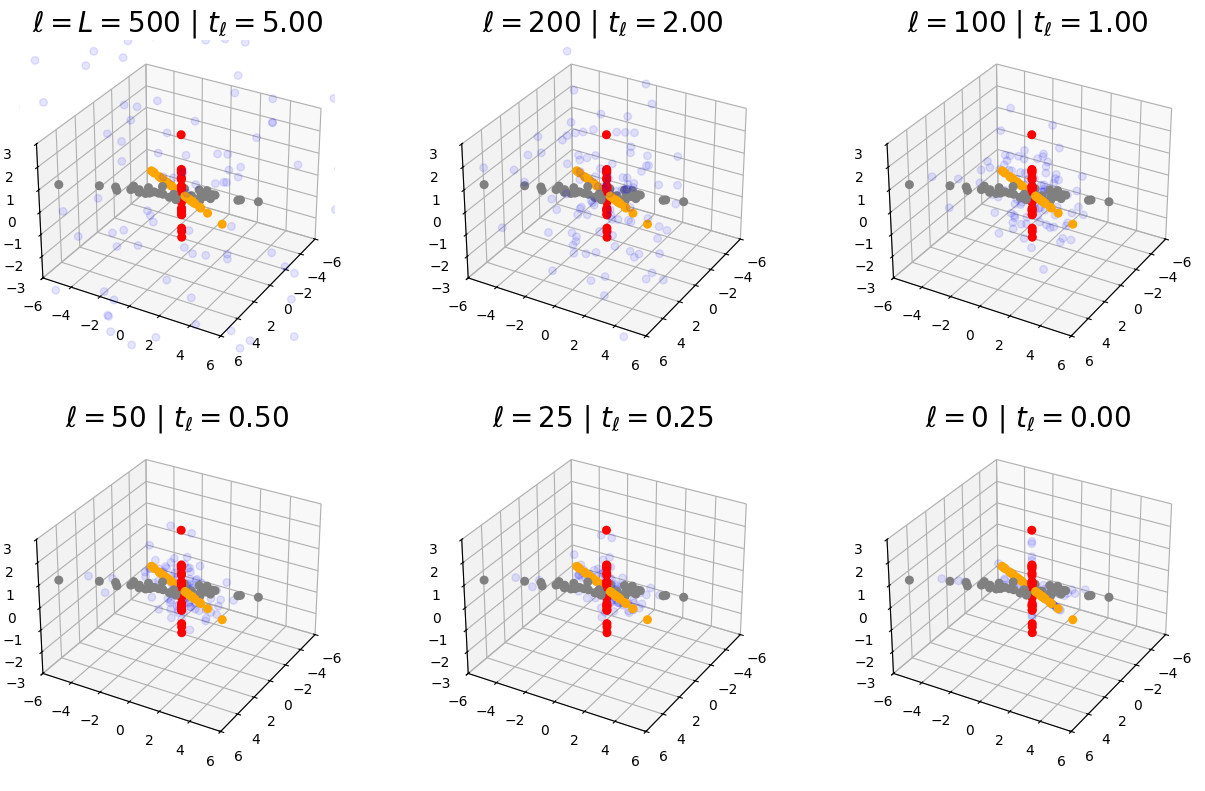
\includegraphics[width=\textwidth]{\toplevelprefix/chapters/chapter3/figs/ve_gmm_denoising.png}
	\caption{\small\textbf{Denoising a low-rank mixture of Gaussians.} Each figure represents samples from the true data distribution (gray, orange, red) and samples undergoing the denoising process \eqref{eq:denoising-iteration-basic} (light blue). At top left, the process has just started, and the noise is very large. As the process continues, the noise is pushed further towards the support of the low-rank data distribution. Finally, in the bottom right, the generated samples are perfectly aligned with the support of the data and look very much like samples drawn from the low-rank Gaussian mixture model.}
	\label{fig:ve_gmm_denoising}
\end{figure}

The above is intuition for why we expect the denoising process to converge. We visualize the convergence process in \(\R^{3}\) in \Cref{fig:ve_gmm_denoising}. We will develop some rigorous results about convergence later. For now, recall that we wanted to build a process to reduce the entropy. While we did do this in a roundabout way by inverting a process which adds entropy, it is now time to pay the piper and confirm that our iterative denoising process reduces the entropy.

\begin{theorem}[Simplified Version of \Cref{thm:conditioning_reduces_entropy}]
	Suppose that \((\vx_{t})_{t \in [0, T]}\) obeys \eqref{eq:additive_gaussian_noise_model}. Then, under certain technical conditions on \(\vx\), for every \(s < t\) with \(s, t \in (0, T]\),
	\begin{equation}
		h(\Ex[\vx_{s} \mid \vx_{t}]) < h(\vx_{t}).
	\end{equation}
\end{theorem}
The full statement of the theorem, and the proof itself, requires some technicality, so it is postponed to \Cref{sub:denoising_entropy_decreases}.

The last thing we discuss here is that many times, we will \textit{not be able to compute} \(\bar{\vx}^{\ast}(t, \cdot)\) for any \(t\), since we do not have the distribution \(p_{t}\). But we can try to \textit{learn one from data}. Recall that the denoiser \(\bar{\vx}^{\ast}\) is defined in \eqref{eq:denoising_loss} as minimizing the mean-squared error \(\Ex\norm{\bar{\vx}(t, \vx_{t}) - \vx}_{2}^{2}\). We can use this mean-squared error as a loss or objective function to learn the denoiser. For example, we can parameterize \(\bar{\vx}(t, \cdot)\) by a neural network, writing it as \(\bar{\vx}_{\theta}(t, \cdot)\), and optimize the loss over the parameter space \(\Theta\):
\begin{equation}
	\min_{\theta \in \Theta}\Ex_{\vx, \vx_{t}}\norm{\bar{\vx}_{\theta}(t, \vx_{t}) - \vx}_{2}^{2}.
\end{equation}
The solution to this optimization problem, implemented via gradient descent or a similar algorithm, will give us a \(\bar{\vx}_{\theta^{\ast}}(t, \cdot)\) which is a good approximation to \(\bar{\vx}^{\ast}(t, \cdot)\) (at least if the training works) and which we will use as our denoiser.

What is a good architecture for this neural network \(\bar{\vx}_{\theta^{\ast}}(t, \cdot)\)? To answer this question, we will examine the ubiquitous case of a \textit{Gaussian mixture model},  whose denoiser we computed in \Cref{example:denoising_gaussian_mixture}. This model is relevant because it can approximate many types of distributions: in particular, given a distribution for \(\vx\), there is a Gaussian mixture model that can approximate it arbitrarily well. So optimizing among the class of denoisers for Gaussian mixture models can give us something close to the optimal denoiser for the real data distribution. 

In our case, we assume that \(\vx\) is low-dimensional, which loosely translates into the requirement that \(\vx\) is \textit{approximately} distributed according to a \textit{mixture of low-rank Gaussians}. Formally, we write 
\begin{equation}\label{eq:MoG1}
	\vx \sim \frac{1}{K}\sum_{k = 1}^{K}\dNorm(\vzero, \vU_{k}\vU_{k}^{\top})
\end{equation}
where \(\vU_{k} \in \O(D, P) \subseteq \R^{D \times P}\) is an orthogonal matrix. Then the optimal denoiser under \eqref{eq:additive_gaussian_noise_model} is (from \Cref{example:denoising_gaussian_mixture})
\begin{equation}
	\bar{\vx}^{\ast}(t, \vx_{t}) = \sum_{k = 1}^{K}\frac{\phi(\vx_{t} ; \vzero,
	\vU_{k}\vU_{k}^{\top} + t^{2}\vI)}{\sum_{i = 1}^{K}\phi(\vx_{t} ; \vzero, \vU_{i}\vU_{i}^{\top} + t^{2}\vI)}\cdot\bp{\vU_{k}\vU_{k}^{\top}(\vU_{k}\vU_{k}^{\top} + t^{2}\vI)^{-1}\vx_{t}}.
\end{equation}
Notice that within the computation \(\phi\) and outside of it, we compute the inverse \((\vU_{k}\vU_{k}^{\top} + t^{2}\vI)^{-1}\). This is a low-rank perturbation of the full-rank matrix \(t^{2}\vI\), and thus ripe for simplification via the \textit{Sherman-Morrison-Woodbury identity}, i.e., for matrices \(\vA, \vC, \vU, \vV\) such that \(\vA\) and \(\vC\) are invertible,
\begin{equation}\label{eq:sherman_morrison_woodbury}
	(\vA + \vU\vC\vV)^{-1} = \vA^{-1} - \vA^{-1}\vU(\vC^{-1} + \vV\vA^{-1}\vU)^{-1}\vV\vA^{-1}.
\end{equation}
We prove this identity in \Cref{exercise:sherman_morrison_woodbury_identity}. For now we apply this identity with \(\vA = t^{2}\vI\), \(\vU = \vU_{k}\), \(\vV = \vU_{k}^{\top}\), and \(\vC = \vI\), obtaining
\begin{align}
	(\vU_{k}\vU_{k}^{\top} + t^{2}\vI)^{-1} 
	&= \frac{1}{t^{2}}\vI - \frac{1}{t^{4}}\vU_{k}\bp{\vI + \frac{1}{t^{2}}\vU_{k}^{\top}\vU_{k}}^{-1}\vU_{k}^{\top} \\
	&= \frac{1}{t^{2}}\vI - \frac{1}{t^{4}\bp{1 + \frac{1}{t^{2}}}}\vU_{k}\vU_{k}^{\top} \\
	&= \frac{1}{t^{2}}\bp{\vI - \frac{1}{1 + t^{2}}\vU_{k}\vU_{k}^{\top}}.
\end{align}
Then we can compute the posterior probabilities as follows. Note that since \(\vU_{k}\)'s are all orthogonal, \(\det(\vU_{k}\vU_{k}^{\top} + t^{2}\vI)\) are all the same for each \(k\). So
\begin{align}
	\frac{\phi(\vx_{t} ; \vzero, \vU_{k}\vU_{k}^{\top} + t^{2}\vI)}{\sum_{i
	= 1}^{K}\phi(\vx_{t} ; \vzero, \vU_{i}\vU_{i}^{\top} + t^{2}\vI)} 
	&= \frac{\exp\rp{-\frac{1}{2}\vx_{t}^{\top}(\vU_{k}\vU_{k}^{\top} + t^{2}\vI)^{-1}\vx_{t}}}{\sum_{i = 1}^{K}\exp\rp{-\frac{1}{2}\vx_{t}^{\top}(\vU_{i}\vU_{i}^{\top} + t^{2}\vI)^{-1}\vx_{t}}} \\
	&= \frac{\exp\rp{-\frac{1}{2t^{2}}\vx_{t}^{\top}\bp{\vI - \frac{1}{1 + t^{2}}\vU_{k}\vU_{k}^{\top}}\vx_{t}}}{\sum_{i = 1}^{K}\exp\rp{-\frac{1}{2t^{2}}\vx_{t}^{\top}\bp{\vI - \frac{1}{1 + t^{2}}\vU_{i}\vU_{i}^{\top}}\vx_{t}}} \\
	&= \frac{\exp\rp{-\frac{1}{2t^{2}}\norm{\vx_{t}}_{2}^{2} + \frac{1}{2t^{2}(1 + t^{2})}\norm{\vU_{k}^{\top}\vx_{t}}_{2}^{2}}}{\sum_{i = 1}^{K}\exp\rp{-\frac{1}{2t^{2}}\norm{\vx_{t}}_{2}^{2} + \frac{1}{2t^{2}(1 + t^{2})}\norm{\vU_{i}^{\top}\vx_{t}}_{2}^{2}}} \\
	&= \frac{\exp\rp{-\frac{1}{2t^{2}}\norm{\vx_{t}}_{2}^{2}}\exp\rp{\frac{1}{2t^{2}(1 + t^{2})}\norm{\vU_{k}^{\top}\vx_{t}}_{2}^{2}}}{\exp\rp{-\frac{1}{2t^{2}}\norm{\vx_{t}}_{2}^{2}}\sum_{i = 1}^{K}\exp\rp{\frac{1}{2t^{2}(1 + t^{2})}\norm{\vU_{i}^{\top}\vx_{t}}_{2}^{2}}} \\
	&= \frac{\exp\rp{\frac{1}{2t^{2}(1 + t^{2})}\norm{\vU_{k}^{\top}\vx_{t}}_{2}^{2}}}{\sum_{i = 1}^{K}\exp\rp{\frac{1}{2t^{2}(1 + t^{2})}\norm{\vU_{i}^{\top}\vx_{t}}_{2}^{2}}}.
\end{align}
This is a softmax operation weighted by the projection of \(\vx_{t}\) onto each subspace measured by \(\norm{\vU_{i}^{\top}\vx_{t}}_{2}\) (tempered by a temperature \(2t^{2}(1 + t^{2})\)). Meanwhile, the component denoisers can be written as 
\begin{align}
	\vU_{k}\vU_{k}^{\top}(\vU_{k}\vU_{k}^{\top} + t^{2}\vI)^{-1}\vx_{t} 
	&= \frac{1}{t^{2}}\vU_{k}\vU_{k}^{\top}\bp{\vI - \frac{1}{1 + t^{2}}\vU_{k}\vU_{k}^{\top}}\vx_{t} \\
	&= \frac{1}{t^{2}}\bp{1 - \frac{1}{1 + t^{2}}}\vU_{k}\vU_{k}^{\top}\vx_{t} \\
	&= \frac{1}{1 + t^{2}}\vU_{k}\vU_{k}^{\top}\vx_{t}.
\end{align}
Putting these together, we have 
\begin{equation}\label{eq:gmm_lowrank_denoiser}
	\bar{\vx}^{\ast}(t, \vx_{t}) = \frac{1}{1 + t^{2}}\sum_{k = 1}^{K}\frac{\exp\rp{\frac{1}{2t^{2}(1 + t^{2})}\norm{\vU_{k}^{\top}\vx_{t}}_{2}^{2}}}{\sum_{i = 1}^{K}\exp\rp{\frac{1}{2t^{2}(1 + t^{2})}\norm{\vU_{i}^{\top}\vx_{t}}_{2}^{2}}}\vU_{k}\vU_{k}^{\top}\vx_{t},
\end{equation}
i.e., a projection of \(\vx_{t}\) onto each of \(K\) subspaces, weighted by a soft-max operation of a quadratic function of \(\vx_{t}\). This functional form is similar to an \textit{attention mechanism} in a transformer architecture! As we will see in \Cref{ch:representation}, this is no coincidence at all; the deep link between denoising and lossy compression (to be covered in \Cref{sec:lossy_compression}) makes transformer denoisers so effective in practice. And so overall, our Gaussian mixture model theory motivates the use of transformer-like neural networks for denoising.

\begin{remark}
{\bf Connections between denoising a distribution and probabilistic PCA.} Here, we would like to connect denoising a low-dimensional distribution to probabilistic PCA (see \Cref{subsec:probabilistic PCA} for more details about probabilistic PCA). Suppose that we consider $K=1$ in \eqref{eq:MoG1}, i.e., $\vx \sim   \dNorm(\vzero, \vU\vU^{\top})$, where \(\vU \in \O(D, P) \subseteq \R^{D \times P}\) is an orthogonal matrix. According to \eqref{eq:gmm_lowrank_denoiser}, the  Bayes optimal denoiser is 
\begin{align}
    \bar{\vx}^{\ast}(t, \vx_{t}) = \frac{1}{1 + t^{2}} \vU\vU^\top\vx_t. 
\end{align}
To learn this Bayes optimal denoiser, we can accordingly parameterize the denoising operator $\bar{\vx}(t,\vx_t)$ as follows: 
\begin{align}
    \bar{\vx}(t,\vx_t) = \frac{1}{1 + t^{2}} \vV\vV^\top\vx_t,
\end{align}
where $\vV \in \O(D, P)$ are learnable parameters. Substituting this into the training loss \eqref{eq:denoising_loss} yields 
\begin{equation}\label{eq:training loss PCA}
	  \min_{\vV \in \O(D, P)}\Ex_{\vx, \vx_{t}}\left\|\vx - \frac{1}{1 + t^{2}} \vV\vV^\top\vx_t\right\|_{2}^{2} = \Ex_{\vx, \vg}\left\|\vx - \frac{1}{1 + t^{2}} \vV\vV^\top(\vx + t\vg)\right\|_{2}^{2},
\end{equation}
where the equality is due to \eqref{eq:additive_gaussian_noise_model}. Conditioned on $\vx$, we compute 
\begin{align}
    & \Ex_{\vg}\left\|\vx - \frac{1}{1 + t^{2}} \vV\vV^\top(\vx + t\vg)\right\|_{2}^{2} \\
    = & \left\|\vx - \frac{1}{1 + t^{2}} \vV\vV^\top \vx\right\|_{2}^{2} - \frac{t}{1+t^2}\Ex_{\vg} \left\langle \vx - \frac{1}{1 + t^{2}} \vV\vV^\top \vx,  \vV\vV^\top\vg \right\rangle + \frac{t^2}{(1+t^2)^2} \Ex_{\vg}\left\| \vV\vV^\top \vg \right\|_2^2 \\
    = & \left\|\vx - \frac{1}{1 + t^{2}} \vV\vV^\top \vx\right\|_{2}^{2} + \frac{t^2P}{(1+t^2)^2} 
\end{align}
where the second equality follows from \(\vg \sim \dNorm(\vzero, \vI)\) and $ \Ex_{\vg}\left\| \vV\vV^\top \vg \right\|_2^2 = \Ex_{\vg}\left\|\vV^\top \vg \right\|_2^2 = P$ due to $\vV \in \O(D, P)$. Therefore, Problem \eqref{eq:training loss PCA} in equivalent to 
\begin{align}
    \min_{\vV \in \O(D, P)}\Ex_{\vx} \left\|\vx - \frac{1}{1 + t^{2}} \vV\vV^\top \vx\right\|_{2}^{2} = \Ex_{\vx} \|\vx\|_2^2 + \left( \frac{1}{(1+t^2)^2} - \frac{2}{1+t^2} \right) \Ex_{\vx}\|\vV^\top \vx\|_2^2.
\end{align}
This is further equivalent to 
\begin{align}
    \max_{\vV \in \O(D, P)} \Ex_{\vx}\|\vV^\top \vx\|_2^2,
\end{align}
which is essentially Problem \eqref{eq:PPCA}. 
\end{remark}

Overall, the learned denoiser forms an (implicit parametric) encoding scheme of the given data, since it can be used to denoise/project onto the data distribution. Training a denoiser is equivalent to finding a better coding scheme, and this partially fulfills one of the desiderata (the \textit{second}) at the end of \Cref{sub:min_entropy}. In the sequel, we will discuss how to fulfill the other (the \textit{first}).


\subsection{Learning and Sampling a Distribution via Iterative Denoising}\label{sub:sampling_denoising}

Remember that at the end of \Cref{sub:min_entropy}, we discussed a pair of desiderata for pursuing a distribution with low-dimensional structure. The first such desideratum is to start with a normal distribution, say with high entropy, and gradually reduce its entropy until it reaches the distribution of the data. We will call this procedure \textit{sampling} since we are generating new samples. It is now time for us to discuss how to do this with the toolkit we have built up.

We know how to denoise very noisy samples \(\vx_{T}\) to attain approximations \(\hat{\vx}\) which have similar distributions to the target random variable \(\vx\). But the desideratum says that, to sample, we want to start with a template distribution with \textit{no} influence from the distribution of \(\vx\), and use the denoiser to guide the iterates towards the distribution of \(\vx\). How can we do this? One way is motivated as follows:
\begin{equation}\label{eq:ve_converge_to_large_gaussian}
	\frac{\vx_{T}}{T} = \frac{\vx + T\vg}{T} = \frac{\vx}{T} + \vg \to \vg \sim \dNorm(\vzero, \vI).
\end{equation}
Thus, \(\vx_{T} \approx \dNorm(\vzero, T^{2}\vI)\). This approximation is quite good for almost all practical distributions, and visualized in \Cref{fig:xT_vs_noise}.
\begin{figure}
	\centering 
	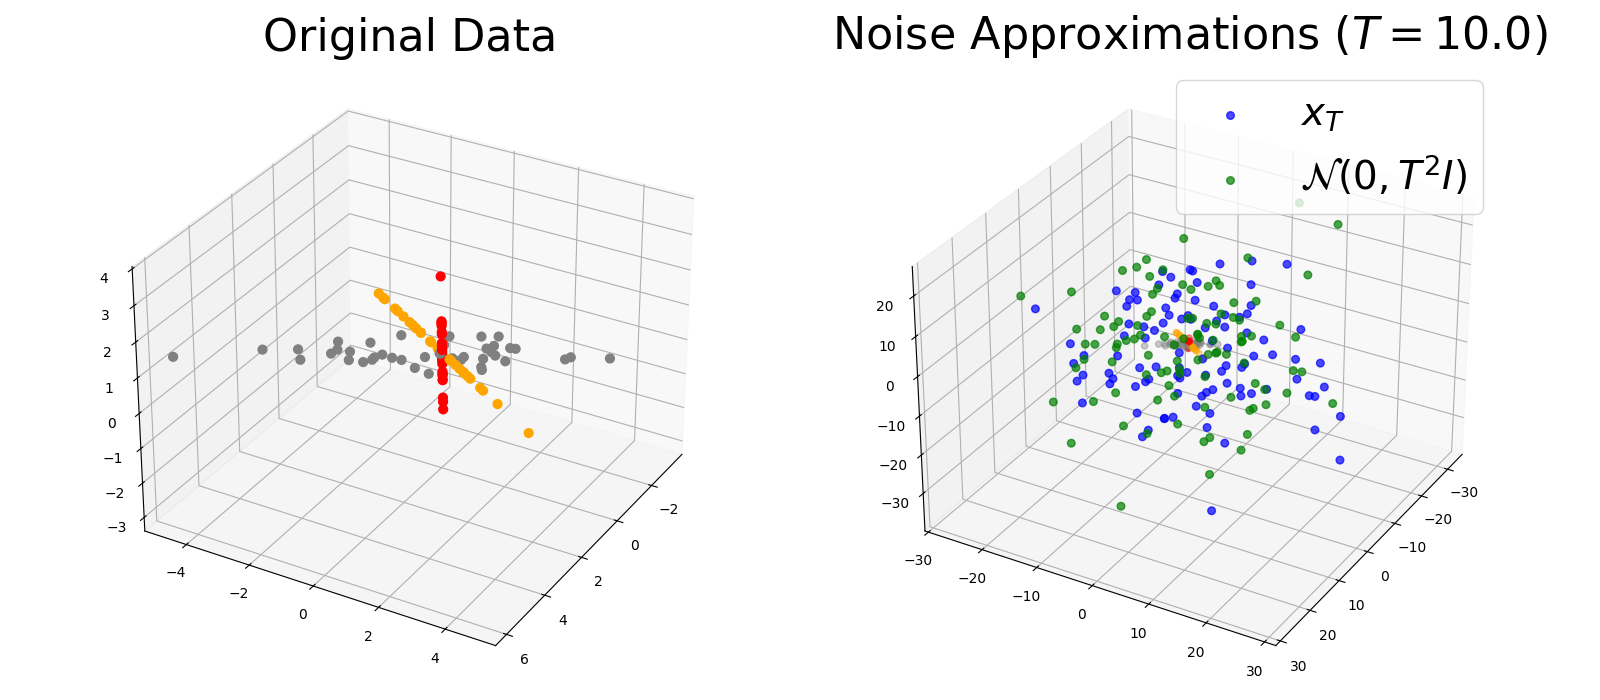
\includegraphics[width=0.75\textwidth]{\toplevelprefix/chapters/chapter3/figs/xT_vs_noise.png}
	\caption{\small\textbf{Visualizing \(\vx_{T}\) versus \(\dNorm(\vzero, T^{2}\vI)\).} \textit{Left:} A plot of Gaussian mixture model data \(\vx\). \textit{Right:} A plot of \(\vx\) as well as \(\vx_{T}\) and an independent sample of \(\dNorm(\vzero, T^{2}\vI)\), for \(T = 10\). On the right plot, \(\vx\) is plotted in the same colors as the left: however, samples from \(\vx_{T}\) and \(\dNorm(\vzero, T^{2}\vI)\) are both much larger, on average, than samples from \(\vx\), and so it appears much smaller because of the scaling. Despite this large blow-up, we clearly observe the similarities in the distributions of \(\vx_{T}\) and \(\dNorm(\vzero, T^{2}\vI)\).}
	\label{fig:xT_vs_noise}
\end{figure}

So, discretizing \([0, T]\) into \(0 = t_{0} < t_{1} < \cdots < t_{L} = T\) uniformly using \(t_{\ell} = T\ell / L\) (as in the previous section), one possible way to sample from pure noise is:
\begin{itemize}
	\item Sample \(\hat{\vx}_{T} \sim \dNorm(\vzero, T^{2}\vI)\) (i.i.d.~of everything else) 
	\item Run the denoising iteration as in \Cref{sub:intro_diffusion_denoising}, i.e.,
		\begin{equation}\label{eq:denoising-iteration-basic}
		\hat{\vx}_{t_{\ell - 1}} = \bp{1 - \frac{1}{\ell}}\cdot\hat{\vx}_{t_{\ell}} + \frac{1}{\ell}\cdot\bar{\vx}^{\ast}(t_{\ell}, \hat{\vx}_{t_{\ell}}).
	\end{equation}
	\item Output \(\hat{\vx} = \hat{\vx}_{0}\).
\end{itemize}
This conceptually is all there is behind \textit{diffusion models}, which transform noise into data samples in accordance with the first desideratum. However, there are a few steps left to take before we get models which can actually sample from real data distributions like images given practical resource constraints. In the sequel, we will introduce and motivate several such steps.

\paragraph{Step 1: different discretizations.} The first step we do is motivated by the following point: \textit{we do not need to spend so many denoising iterations} at large  \(t\). If we look at \Cref{fig:ve_gmm_denoising}, we observe that the first \(200\) or \(300\) iterations, out of the \(500\) iterations of the sampling process, are just spent contracting the noise towards the data distribution as a whole, before the remaining iterations push the samples towards a subspace. Given a fixed iteration count \(L\), this signals that we should spend more timesteps \(t_{\ell}\) near \(t = 0\) compared to \(t = T\). During sampling (and training), we can therefore use another discretization of \([0, T]\) into \(0 \leq t_{0} < t_{1} < \cdots < t_{L} \leq T\), such as an \textit{exponential discretization}:
\begin{equation}\label{eq:denoising_exponential_discretization}
	t_{\ell} = C_{1}(e^{C_{2}\ell} - 1), \qquad \forall \ell \in \{0, 1, \dots, L\}
\end{equation}
where \(C_{1}, C_{2} > 0\) are constants which can be tuned for optimal performance in practice; theoretical analysis will often specify such optimal constants as well. Then the denoising/sampling iteration becomes 
\begin{equation}\label{eq:denoising_iteration}
	\hat{\vx}_{t_{\ell - 1}} \doteq \frac{t_{\ell - 1}}{t_{\ell}}\hat{\vx}_{t_{\ell}} + \bp{1 - \frac{t_{\ell - 1}}{t_{\ell}}}\bar{\vx}^{\ast}(t_{\ell}, \hat{\vx}_{t_{\ell}}),
\end{equation}
with, again, \(\hat{\vx}_{t_{L}} \sim \dNorm(\vzero, t_{L}^{2}\vI)\).

\paragraph{Step 2: different noise models.} The second step is to consider slightly different models compared to \eqref{eq:additive_gaussian_noise_model}. The basic motivation for this is as follows. In practice, the noise distribution \(\dNorm(\vzero, t_{L}^{2}\vI)\) becomes an increasingly poor estimate of the true covariance in high dimensions, i.e., \eqref{eq:ve_converge_to_large_gaussian} becomes an increasingly worse approximation, especially with anisotropic high-dimensional data. The increased distance between \(\dNorm(\vzero, t_{L}^{2}\vI)\) and the true distribution of \(\vx_{t_{L}}\) may cause the denoiser to perform worse in such circumstances. Theoretically, \(\vx_{t_{L}}\) never converges to any distribution as \(t_{L}\) increases, so this setup is difficult to analyze end-to-end. In this case, our remedy is to \textit{simultaneously add noise and shrink the contribution of \(\vx\), such that \(\vx_{T}\) converges as \(T \to \infty\)}. The rate of added noise is denoted \(\sigma \colon [0, T] \to \R_{\geq 0}\), and the rate of shrinkage is denoted \(\alpha \colon [0, T] \to \R_{\geq 0}\), such that \(\sigma\) is \textit{increasing} and \(\alpha\) is (not strictly) \textit{decreasing}, and 
\begin{equation}\label{eq:gen_additive_gaussian_noise_model}
	\vx_{t} \doteq \alpha_{t}\vx + \sigma_{t}\vg, \qquad \forall t \in [0, T].
\end{equation}
The previous setup has \(\alpha_{t} = 1\) and \(\sigma_{t} = t\), and this is called the \textit{variance-exploding (VE) process}. A popular choice which decreases the contribution of \(\vx\), as we described originally, has \(T = 1\) (so that \(t \in [0, 1]\)), \(\alpha_{t} = \sqrt{1 - t^{2}}\) and \(\sigma_{t} = t\); this is the \textit{variance-preserving (VP) process}. Note that under the VP process, \(\vx_{1} \sim \dNorm(\vzero, \vI)\) exactly, so we can just sample from this standard distribution and iteratively denoise. As a result, the VP process is much easier to analyze theoretically and more stable empirically.\footnote{Why use the whole \(\alpha, \sigma\) setup? As we will see in \Cref{exercise:implement_denoising_processes}, it encapsulates and unifies many proposed processes, including the recently popular so-called \textit{flow matching} process. Despite this, the VE and VP processes are still the most popular empirically and theoretically (so far), and so we will consider them in this Section.} 

With this more general setup, Tweedie's formula \eqref{eq:tweedie} becomes 
\begin{equation}\label{eq:gen_tweedie}
	\Ex[\vx \mid \vx_{t}] = \frac{1}{\alpha_{t}}\bp{\vx_{t} + \sigma_{t}^{2}\nabla \log p_{t}(\vx)}.
\end{equation}
The denoising iteration \eqref{eq:denoising_iteration} becomes
\begin{equation}\label{eq:gen_denoising_iteration}
	\hat{\vx}_{t_{\ell - 1}} = \frac{\sigma_{t_{\ell - 1}}}{\sigma_{t_{\ell}}}\hat{\vx}_{t_{\ell}} + \bp{\alpha_{t_{\ell - 1}} - \frac{\sigma_{t_{\ell - 1}}}{\sigma_{t_{\ell}}}\alpha_{t_{\ell}}}\bar{\vx}^{\ast}(t_{\ell}, \hat{\vx}_{t_{\ell}}).
\end{equation}
Finally, the Gaussian mixture model denoiser \eqref{eq:gmm_bayes_optimal_denoiser} becomes 
\begin{equation}\label{eq:gen_gmm_bayes_optimal_denoiser}
	\bar{\vx}^{\ast}(t, \vx_{t}) = \sum_{k = 1}^{K}\frac{\pi_{k}\phi(\vx_{t}
	; \alpha_{t}\vmu_{k}, \alpha_{t}^{2}\vSigma_{k}
	+ \sigma_{t}^{2}\vI)}{\sum_{i = 1}^{K}\pi_{i}\phi(\vx_{t} ; \alpha_{t}\vmu_{i}, \alpha_{t}^{2}\vSigma_{i} + \sigma_{t}^{2}\vI)}\cdot\bp{\vmu_{k} + \alpha_{t}\vSigma_{k}(\alpha_{t}^{2}\vSigma_{k} + \sigma_{t}^{2}\vI)^{-1}(\vx_{t} - \alpha_{t}\vmu_{k})}.
\end{equation}
\Cref{fig:vp_gmm_denoising} demonstrates iterations of the sampling procedure. Note that the denoising iteration \eqref{eq:gen_denoising_iteration} gives a sampling algorithm called the DDIM (``Denoising Diffusion Implicit Model'') sampler \cite{song2020denoising}, and is one of the most popular sampling algorithms used today in diffusion models. We summarize it here in \Cref{alg:iterative_denoising}.

\begin{figure}
	\centering 
	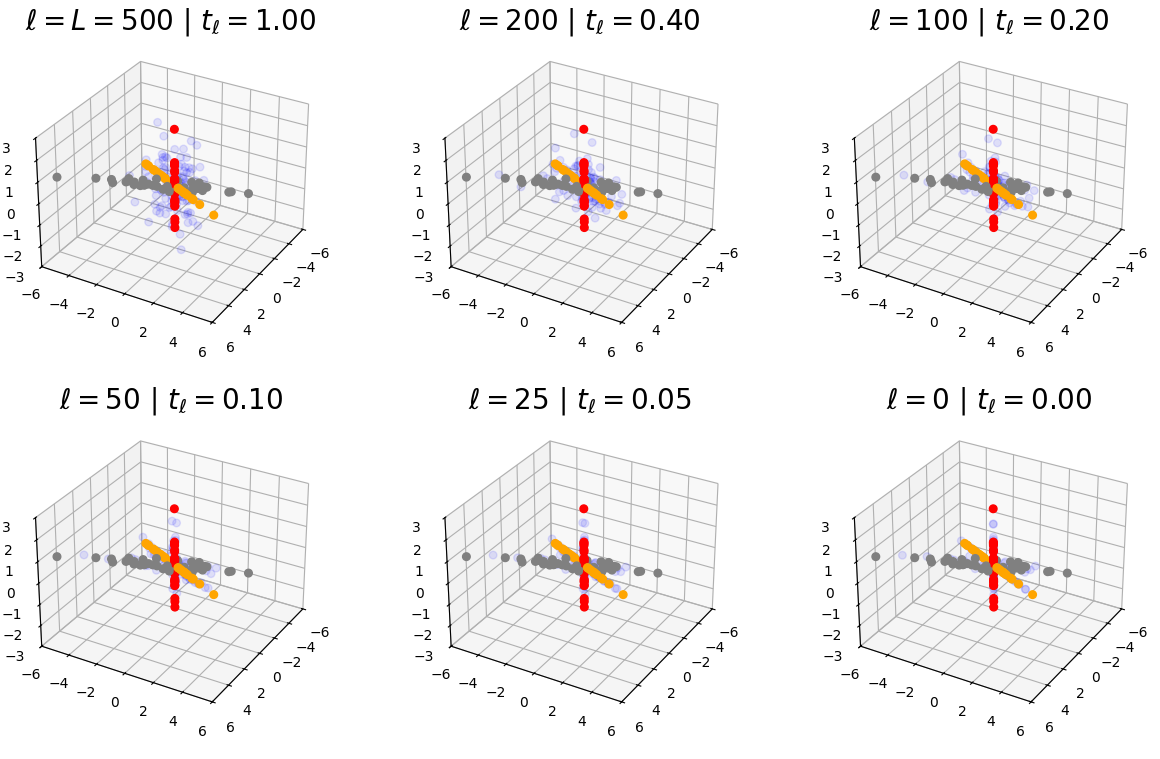
\includegraphics[width=\textwidth]{\toplevelprefix/chapters/chapter3/figs/vp_gmm_denoising.png}
	\caption{\small\textbf{Denoising a mixture of Gaussians using the VP diffusion process.} We use the same figure setup and data distribution as \Cref{fig:ve_gmm_denoising}. Note that compared to \Cref{fig:ve_gmm_denoising}, the noise distribution is much more concentrated around the origin.}
	\label{fig:vp_gmm_denoising}
\end{figure}

\begin{algorithm}
	\caption{Sampling using a denoiser.}
	\label{alg:iterative_denoising}
	\begin{algorithmic}[1]
		\Require{An ordered list of timesteps \(0 \leq t_{0} < \cdots < t_{L} \leq T\) to use for sampling.}
		\Require{A denoiser \(\bar{\vx} \colon \{t_{\ell}\}_{\ell = 1}^{L} \times \R^{D} \to \R^{D}\).}
		\Require{Scale and noise level functions \(\alpha, \sigma \colon \{t_{\ell}\}_{\ell = 0}^{L} \to \R_{\geq 0}\).}
		\Ensure{A sample \(\hat{\vx}\), approximately from the distribution of \(\vx\).}
		\Function{DDIMSampler}{$\bar{\vx}, (t_{\ell})_{\ell = 0}^{L}$}
		\State{Initialize \(\tilde{\vx}_{t_{L}} \sim\) approximate distribution of \(\vx_{t_{L}}\)} \Comment{VP \(\implies \dNorm(\vzero, \vI)\), VE \(\implies \dNorm(\vzero, t_{L}^{2}\vI)\).}
		\For{\(\ell = L, L - 1, \dots, 1\)}
		\State{Compute
			\begin{equation*}
				\hat{\vx}_{t_{\ell - 1}} \doteq \frac{\sigma_{t_{\ell - 1}}}{\sigma_{t_{\ell}}}\hat{\vx}_{t_{\ell}} + \bp{\alpha_{t_{\ell - 1}} - \frac{\sigma_{t_{\ell - 1}}}{\sigma_{t_{\ell}}}\alpha_{t_{\ell}}}\bar{\vx}(t_{\ell}, \hat{\vx}_{t_{\ell}})
			\end{equation*}
		}
		\EndFor
		\State{\Return{\(\hat{\vx}_{t_{0}}\)}}
		\EndFunction
	\end{algorithmic}
\end{algorithm}

\paragraph{Step 3: optimizing training pipelines.} If we use the procedure dictated by \Cref{sub:intro_diffusion_denoising} to learn a separate denoiser \(\bar{\vx}(t, \cdot)\) for each time \(t\) to be used in the sampling algorithm, \textit{we would have to learn \(L\) separate denoisers!} This is highly inefficient---the usual case is that we have to train \(L\) separate neural networks, taking up \(L\) times the training time and storage memory, and then be locked into using these timesteps for sampling forever. Instead, we can \textit{train a single neural network} to denoise across all times \(t\), taking as input the continuous variables \(\vx_{t}\) and \(t\) (instead of just \(\vx_{t}\) before). Mechanically, our training loss averages over \(t\), i.e., solves the following problem:
\begin{equation}
	\min_{\theta}\Ex_{t, \vx, \vx_{t}}\norm{\bar{\vx}_{\theta}(t, \vx_{t}) - \vx}_{2}^{2}.
\end{equation}
Similar to Step 1, where we used more timesteps closer to \(t = 0\) to ensure a better sampling process, we may want to ensure that the denoiser is higher quality closer to \(t = 0\), and thereby \textit{weight the loss} so that \(t\) near \(0\) has higher weight. Letting \(w_{t}\) be the weight at time \(t\), the weighted loss would look like
\begin{equation}\label{eq:parametric_denoising_loss}
	\min_{\theta}\Ex_{t}w_{t}\Ex_{\vx, \vx_{t}}\norm{\bar{\vx}_{\theta}(t, \vx_{t}) - \vx}_{2}^{2}.
\end{equation}
One reasonable choice of weight in practice is \(w_{t} = \alpha_{t}/\sigma_{t}\). The precise reason will be covered in the next paragraph, but generally it serves to up-weight the losses corresponding to \(t\) near \(0\) while still remaining reasonably numerically stable. Also, of course, we cannot compute the expectation in practice, so we use the most straightforward Monte-Carlo average to estimate it. The series of changes made here have several conceptual and computational benefits: we do not need to train multiple denoisers, we can train on one set of timesteps and sample using a subset (or others entirely), etc. The full pipeline is discussed in \Cref{alg:learning_denoiser}.

\begin{algorithm}
	\begin{algorithmic}[1]
		\Require{Dataset \(\cD \subseteq \R^{D}\).}
		\Require{An ordered list of timesteps \(0 \leq t_{0} < \cdots < t_{L} \leq T\) to use for sampling.}
		\Require{A weighting function \(w \colon \{t_{\ell}\}_{\ell = 1}^{L} \to \R_{\geq 0}\).}
		\Require{Scale and noise level functions \(\alpha, \sigma \colon \{t_{\ell}\}_{\ell = 0}^{L} \to \R_{\geq 0}\).}
		\Require{A parameter space \(\Theta\) and a denoiser architecture \(\bar{\vx}_{\theta}\).}
		\Require{An optimization algorithm for the parameters.}
		\Require{The number of optimization iterations \(M\).}
		\Require{The number of Monte-Carlo draws \(N\) per iteration (to approximate the expectation in \eqref{eq:parametric_denoising_loss})}
		\Ensure{A trained denoiser \(\bar{\vx}_{\theta^{\ast}}\).}

		\Function{TrainDenoiser}{$\cD, \Theta$}
		\State{Initialize \(\theta^{(1)} \in \Theta\)}
		\For{\(i \in [M]\)}
		\For{\(n \in [N]\)}
		\State{\(\vx_{n}^{(i)} \sim \cD\)} \Comment{Draw a sample from the dataset.}
		\State{\(t_{n}^{(i)} \simiid \dUnif(\{t_{\ell}\}_{\ell = 1}^{L})\)} \Comment{Sample a timestep.}
		\State{\(\vg_{n}^{(i)} \simiid \dNorm(\vzero, \vI)\)} \Comment{Sample a noise vector.}
		\State{\(\vx_{t, n}^{(i)} \doteq \alpha_{t_{n}^{(i)}}\vx_{n}^{(i)} + \sigma_{t_{n}^{(i)}}\vg_{n}^{(i)}\)} \Comment{Compute the noised sample.}
		\State{\(w_{n}^{(i)} \doteq w_{t_{n}^{(i)}}\)} \Comment{Compute the loss weight.}
		\EndFor
		\State{\(\hat{\cL}^{(i)} \doteq \displaystyle \frac{1}{N}\sum_{n = 1}^{N}w_{n}^{(i)}\norm{\vx_{n}^{(i)} - \bar{\vx}_{\theta^{(i)}}(t_{n}^{(i)}, \vx_{t, n}^{(i)})}_{2}^{2}\)} \Comment{Compute the loss estimate.}
		\State{\(\theta^{(i + 1)} \doteq \texttt{OptimizationUpdate}^{(i)}(\theta^{(i)}, \nabla_{\theta^{(i)}}\hat{\cL}^{(i)})\)} \Comment{Update parameters.}
		\EndFor
		\State{\Return{\(\bar{\vx}_{\theta^{(K + 1)}}\)}}
		\EndFunction
	\end{algorithmic}
	\caption{Learning a denoiser from data.}
	\label{alg:learning_denoiser}
\end{algorithm}

\paragraph{(Optional) Step 4: changing the estimation target.} Note that it is common to instead reorient the whole denoising pipeline around \textit{noise predictors}, i.e., estimates of \(\Ex[\vg \mid \vx_{t}]\). In practice, noise predictors are slightly easier to train because their output is (almost) always of comparable size to a Gaussian random variable, so training is more numerically stable. Note that by \eqref{eq:gen_additive_gaussian_noise_model} we have 
\begin{equation}
	\vx_{t} = \alpha_{t}\Ex[\vx \mid \vx_{t}] + \sigma_{t}\Ex[\vg \mid \vx_{t}] \implies \Ex[\vg \mid \vx_{t}] = \frac{1}{\sigma_{t}}\bp{\vx_{t} - \alpha_{t}\Ex[\vx \mid \vx_{t}]},
\end{equation}
Therefore any predictor for \(\vx\) can be turned into a predictor for \(\vg\) using the above relation, i.e.,
\begin{equation}
	\bar{\vg}(t, \vx_{t}) = \frac{1}{\sigma_{t}}\vx_{t} - \frac{\alpha_{t}}{\sigma_{t}}\bar{\vx}(t, \vx_{t}),
\end{equation}
and vice-versa. Thus a good network for estimating \(\bar{\vg}\) is the same as a good network for estimating \(\bar{\vx}\) \textit{plus a residual connection} (as seen in, e.g., transformers). Their losses are also the same as the denoiser, up to the factor of \(\alpha_{t}/\sigma_{t}\), i.e.,
\begin{equation}
	\Ex_{t}w_{t}\Ex_{\vg, \vx_{t}}\norm{\vg - \bar{\vg}(t, \vx_{t})}_{2}^{2} = \Ex_{t}w_{t}\frac{\alpha_{t}^{2}}{\sigma_{t}^{2}}\Ex_{\vx, \vx_{t}}\norm{\vx - \bar{\vx}(t, \vx_{t})}_{2}^{2}.
\end{equation}
For the sake of completeness we will mention that other targets have been proposed for different tasks, e.g., \(\Ex[\odv*{\vx_{t}}{t} \mid \vx_{t}]\) (called \(v\)-prediction or velocity prediction), etc., but denoising and noise prediction remain commonly used. Throughout the rest of this book we will only consider denoising.


We have made lots of changes to our original platonic noising/denoising process. To assure ourselves that the new process still works in practice, we can compute numerical examples (such as \Cref{fig:vp_gmm_denoising}). To assure ourselves that it is theoretically sound, we can prove a \textit{bound on the error rate} for the sampling algorithm, which shows that the error rate is small. We will now furnish such a rate from the literature, which shows that the output distribution of the sampler converges in the so-called \textit{total variation (TV) distance} to the true distribution. The TV distance is defined between two random variables \(\vx\) and \(\vy\) as:
\begin{equation}
	\TV(\vx, \vy) \doteq \sup_{A \subseteq \R^{d}}\abs*{\Pr[\vx \in A] - \Pr[\vy \in A]}.
\end{equation}
If \(\vx\) and \(\vy\) are very close (uniformly), then the supremum will be small. So the TV distance measures the closeness of random variables. (It is indeed a metric, as the name suggests: the proof is an exercise.)

\begin{theorem}[\citep{li2024d} Theorem 1, Simplified]\label{thm:diffusion_sampler_convergence}
	Suppose that \(\Ex\norm{\vx}_{2} < \infty\).  If \(\vx\) is denoised according to the VP process with an exponential discretization\footnote{The precise definition is rather lengthy in our notation and only defined up to various absolute constants, so we omit it here for brevity. Of course it is in the original paper \citep{li2024d}.} as in \eqref{eq:denoising_exponential_discretization}, the output \(\hat{\vx}\) of \Cref{alg:iterative_denoising} satisfies the total variation bound
	\begin{equation}\label{eq:diffusion_sampling_error}
		\TV(\vx, \hat{\vx}) = \tilde{\cO}\rp{\underbrace{\frac{D}{L}}_{\text{discretization error}} + \underbrace{\sqrt{\frac{1}{L}\sum_{\ell = 1}^{L}\frac{\alpha_{t_{\ell}}}{\sigma_{t_{\ell}}^{2}}\Ex_{\vx, \vx_{t_{\ell}}}\norm{\bar{\vx}^{\ast}(t_{\ell}, \vx_{t_{\ell}}) - \bar{\vx}(t_{\ell}, \vx_{t_{\ell}})}_{2}^{2}}}_{\text{average excess error of the denoiser}}}
	\end{equation}
	where \(\bar{\vx}^{\ast}\) is the Bayes optimal denoiser for \(\vx\), and \(\tilde{\cO}\) is a version of the big-\(\cO\) notation which ignores logarithmic factors in \(L\).
\end{theorem}
The very high-level proof technique is, as discussed earlier, to bound the error at each step, distinguish the error sources (between discretization and denoiser error) and carefully ensure that the errors do not accumulate too much (or even cancel out). 

Note that, if \(L \to \infty\) and we correctly learn the Bayes optimal denoiser \(\bar{\vx} = \bar{\vx}^{\ast}\) (such that the excess error is \(0\)), then the sampling process in \Cref{alg:iterative_denoising} yields a \textit{perfect (in distribution) inverse} of the noising process, since the error rate in \Cref{thm:diffusion_sampler_convergence} goes to \(0\),\footnote{There are similar results for VE processes, though none are as sharp as this to our knowledge.} as heuristically argued previously.

\begin{remark}
	What if the data is low-dimensional, say supported on a \textit{low-rank subspace} of the high dimensional space \(\R^{D}\)? If the data distribution is compactly supported---say if the data is normalized to the unit hypercube, which is often ensured as a pre-processing step for real data such as images---it is possible to do better. Namely, the authors of \cite{li2024d} also define a measure of \textit{approximate intrinsic dimension} using the asymptotics of the so-called covering number, which is extremely similar in intuition (if not in implementation) to the rate distortion function presented in the next Section. Then they show that using a particular small modification of the DDIM sampler in \Cref{alg:iterative_denoising} (i.e., slightly perturbing the update coefficients), the discretization error becomes
	\begin{equation}
		\tilde{\cO}\rp{\frac{\text{approximate intrinsic dimension}}{L}}
	\end{equation}
	instead of \(\frac{D}{L}\) like it was in \Cref{thm:diffusion_sampler_convergence}. Therefore, using this modified algorithm, \(L\) does not have to be too large even as \(D\) reaches the thousands or millions, since real data has low-dimensional structure. However in practice we use the DDIM sampler instead, so \(L\) should have a mild dependence on \(D\) to achieve consistent error rates. The exact choice of \(L\) trades off between the computational complexity (e.g., runtime or memory consumption) of sampling and the statistical complexity of learning a denoiser for low-dimensional structures. The value of \(L\) is often different at training time (where a larger \(L\) allows better coverage of the interval \([0, T]\), which helps the network learn a relationship which generalizes over \(t\)) and sampling time (where \(L\) being smaller means more efficient sampling). One can even pick the timesteps adaptively at sampling time in order to optimize this tradeoffs \cite{bao2022analytic}.
\end{remark}

\begin{remark}
	Various other works define the reverse process as moving backward in the time index \(t\) using an explicit difference equation, or differential equation in the limit \(L \to \infty\), or forward in time using the transformation \(\vy_{t} = \vx_{T - t}\), such that if \(t\) increases then \(\vy_{t}\) becomes closer to \(\vx_{0}\). In this work we strive to keep consistency: we move forward in time to noise, and backward in time to denoise. If you are reading another work which is not clear on the time index, or trying to implement an algorithm which is similarly unclear, there is one way to do it right every time: the sampling process should always have a \textit{positive} coefficient on both the denoiser term and the current iterate when moving from step to step. But in general many papers define their own notation and it is not user-friendly.
\end{remark}

\begin{remark}
	The theory presented at the end of the last \Cref{sub:intro_diffusion_denoising} seems to suggest (loosely speaking) that in practice, using a transformer-like network is a good choice for learning or approximating a denoiser. This is reasonable, but what is the problem with using any old neural network (such as a multi-layer perceptron (MLP)) and just trying to scale it up to infinity? To observe the problem with this, let us look at another special case of the Gaussian mixture model studied in \Cref{example:denoising_gaussian_mixture}. Namely, the \textit{empirical distribution} is an instance of a degenerate Gaussian mixture model, with \(K = N\) components \(\dNorm(\vx_{i}, \vzero)\) sampled with equal probability \(\pi_{i} = \frac{1}{N}\). In this case the Bayes optimal denoiser is
	\begin{equation}\label{eq:memorizing_denoiser}
		\bar{\vx}^{\star}(t, \vx_{t}) = \sum_{i = 1}^{N}\frac{e^{-\|\vx_{t} - \alpha_{t}\vx_{i}\|_{2}^{2}/(2\sigma_{t}^{2})}}{\sum_{j = 1}^{N}e^{-\|\vx_{t} - \alpha_{t}\vx_{j}\|_{2}^{2}/(2\sigma_{t}^{2})}}\vx_{i}.
	\end{equation}
	This is a convex combination of the data \(\vx_{i}\), and the coefficients get ``sharper'' (i.e., closer to \(0\) or \(1\)) as \(t \to 0\). Notice that this denoiser \textit{optimally solves} the denoising optimization problem \eqref{eq:parametric_denoising_loss} when we compute the loss based on drawing \(\vx\) uniformly at random from a fixed finite dataset \(\vX = \{\vx_{i}\}_{i = 1}^{N}\), which is a very realistic setting. Thus, if our network architecture \(\bar{\vx}_{\theta}\) is expressive enough such that optimal denoisers of the above form \eqref{eq:memorizing_denoiser} may be well-approximated, then the learned denoiser may do just that. Then, our iterative denoising \Cref{alg:iterative_denoising} will sample exactly from the empirical distribution, re-generating samples in the training data, as certified by \Cref{thm:diffusion_sampler_convergence}. This is a bad sampler, not really more interesting than a database of all samples, and so it is important to understand how to avoid this in practice. The key is to come up with a network architecture which can well-approximate the true denoiser (say corresponding to a low-rank distribution as in \eqref{eq:gmm_lowrank_denoiser}) but not the empirical Bayesian denoiser as in \eqref{eq:memorizing_denoiser}. Some work has explored this fine line and why modern diffusion models, which use transformer- and convolutional-based network architectures, can memorize and generalize in different regimes \citep{kamb2024analytic,niedoba2024towards}.

	At a high level, a denoiser which memorizes all the training points, as in \eqref{eq:memorizing_denoiser}, corresponds to a parametric model of the distribution which has minimal coding rate, and achieves this by just coding every sample separately. We will discuss this problem (and seeming paradox with our initial desiderata at the end of \Cref{sub:min_entropy}) from the perspective of information theory in the next section.
\end{remark}




% \subsubsection{Denoising, and Learning a Denoiser}

% , say within a function class \(\cF_{t}\) of square-integrable functions from \(\R^{D}\) to \(\R^{D}\), which forms the best possible approximation (on average) of the true \(\vx\), given \(t\) and \(\vx_{t}\):
% \begin{equation}\label{eq:denoising_loss_one_t}
% 	\bar{\vx}^{\ast}(t, \cdot) \in \argmin_{\bar{\vx}(t, \cdot) \in \cF_{t}}\Ex_{\vx, \vx_{t}}\norm{\vx - \bar{\vx}(t, \vx_{t})}_{2}^{2}.
% \end{equation}
% In short, the solution to the denoising problem is a \textit{denoiser}: a map which attempts to remove all the noise (and inverts the scaling) from the noisy random variable \(\vx_{t}\) to get an approximation to \(\vx\). As the notation suggests, we can also attempt to learn a denoiser which \textit{jointly} denoises from all times \(t\) simultaneously. Namely, given a distribution of \(t\)'s, a weighting function \(w \colon [0, T] \to \R_{\geq 0}\), and a function class \(\cF\) of square-integrable functions from \([0, T] \times \R^{D}\) to \(\R^{D}\), we can attempt to learn a denoiser from this function class:
% \begin{equation}\label{eq:denoising_loss_all_t}
% 	\bar{\vx}^{\ast} \in \argmin_{\bar{\vx} \in \cF}\Ex_{t, \vx, \vx_{t}}w_{t}\norm{\vx - \bar{\vx}(t, \vx_{t})}_{2}^{2}.
% \end{equation}
% The function classes \(\cF_{t}\) and \(\cF\) can be variously defined. For instance, when \(\cF_{t}\) or \(\cF\) is the whole set of square-integrable functions, we obtain an analytically tractable solution in the \textit{Bayes optimal denoiser}:
% \begin{equation}\label{eq:optimal_denoiser}
% 	\bar{\vx}^{\ast}(t, \vxi) \doteq \Ex[\vx \mid \vx_{t} = \vxi].
% \end{equation}
% Indeed, this notation is why it is justified to use the notation \(\bar{\vx}\) as the Bayes optimal denoiser computes a conditional expectation (i.e., conditional average or mean).
% \yima{Why not introduce the Tweedie's formula and property here already?... and then describe how to compute it?}


% Of course, in practice it is impossible to actually compute this conditional expectation without perfect knowledge of the distribution of \(\vx\) (and even then it may still be intractable). So in practice we look to the second case where the denoiser is parameterized, say \(\cF = \{f_{\theta} \colon \theta \in \Theta\}\) where \(\Theta\) is the parameter space. Formally, we can train such denoisers using the method in \Cref{alg:learning_denoiser}.

% So the question is, what is a good parametric function family \(\cF\)? For special cases of distributions, such as Gaussians, a functional form containing the optimal denoiser can be explicitly derived.

% \yima{Please change the environment for Example to something similar to proof, with a QED mark so that we know when an example is finished.}
% \begin{example}[Denoising Gaussian Noise from a Gaussian Mixture Model]\label{example:gmm_denoising}
% 	Suppose that \(\vx\) has the following data-generating process:
% 	\begin{itemize}
% 		\item First, an auxiliary (``label'') variable \(y\) is sampled according to the probability vector \(\vpi\), that is, \(y = k \in [K]\) with probability \(\pi_{k}\).
% 		\item Then, \(\vx\) is sampled as \(\vx \sim \dNorm(\vmu_{y}, \vSigma_{y})\).
% 	\end{itemize}
% 	Marginally, \(\vx\) is a Gaussian Mixture Model, namely
% 	\begin{equation}
% 		\vx \sim \sum_{k = 1}^{K}\pi_{k}\dNorm(\vmu_{k}, \vSigma_{k}).
% 	\end{equation}
% 	Then it is easy to see that
% 	\begin{equation}
% 		\vx_{t} \sim \sum_{k = 1}^{K}\pi_{k}\dNorm(\alpha_{t}\vmu_{k}, \alpha_{t}^{2}\vSigma_{k} + \sigma_{t}^{2}\vI).
% 	\end{equation}
% 	Conditioned on the label \(y\), the variables \(\vx\) and \(\vx_{t}\) are jointly Gaussian, i.e.,
% 	\begin{equation}
% 		\mat{\vx \\ \vx_{t}} \mid y \sim \dNorm\rp{\mat{\vmu_{y} \\ \alpha_{t}\vmu_{y}}, \mat{\vSigma_{y} & \alpha_{t}\vSigma_{y} \\ \alpha_{t}\vSigma_{y} & \alpha_{t}^{2}\vSigma_{y} + \sigma_{t}^{2}\vI}},
% 	\end{equation}
% 	and the posterior distribution of \(\vx\) given \(\vx_{t}\) and \(y\) is (famously)
% 	\begin{equation}
% 		\vx \mid (\vx_{t}, y) \sim \dNorm(\vmu_{y} + \alpha_{t}\vSigma_{y}(\alpha_{t}^{2}\vSigma_{y} + \sigma_{t}^{2}\vI)^{-1}(\vx_{t} - \alpha_{t}\vmu_{y}), \vSigma_{y} - \alpha_{t}^{2}\vSigma_{y}(\alpha_{t}^{2}\vSigma_{y} + \sigma_{t}^{2}\vI)^{-1}\vSigma_{y}).
% 	\end{equation}
% 	Then the optimal denoiser (among all square-integrable functions) given the label \(y\) is the conditional expectation:
% 	\begin{equation}\label{eq:gaussian_denoiser}
% 		\Ex[\vx \mid \vx_{t}, y] = \vmu_{y} + \alpha_{t}\vSigma_{y}(\alpha_{t}^{2}\vSigma_{y} + \sigma_{t}^{2}\vI)^{-1}(\vx_{t} - \alpha_{t}\vmu_{y}).
% 	\end{equation}
% 	To find the Bayes optimal denoiser \(\bar{\vx}^{\star}(t, \cdot) = \Ex[\vx \mid \vx_{t}]\), we use iterated expectation:
% 	\begin{align}
% 		\bar{\vx}^{\star}(t, \vx_{t})
% 		 & = \Ex[\Ex[\vx \mid \vx_{t}, y] \mid \vx_{t}]                         \\
% 		 & = \sum_{k = 1}^{K}\Ex[\vx \mid \vx_{t}, y = k]p(y = k \mid \vx_{t}).
% 	\end{align}
% 	Let \(\phi(\vx \mid \vmu, \vSigma)\) be the density of a Gaussian random variable with mean \(\vmu\) and covariance \(\vSigma\) evaluated at \(\vx\). By Bayes' rule we can calculate the latter as:
% 	\begin{align}
% 		p(y = k \mid \vx_{t})
% 		 & = \frac{p(\vx_{t} \mid y = k)p(y = k)}{\sum_{i = 1}^{K}p(\vx_{t} \mid y = i)p(y = i)}                                                                                                                                \\
% 		 & = \frac{\pi_{k} p(\vx_{t} \mid y = k)}{\sum_{i = 1}^{K}\pi_{i} p(\vx_{t} \mid y = i)}                                                                                                                                \\
% 		 & = \frac{\pi_{k} \phi(\vx_{t} \mid \alpha_{t}\vmu_{k}, \alpha_{t}^{2}\vSigma_{k} + \sigma_{t}^{2}\vI)}{\sum_{i = 1}^{K}\pi_{i} \phi(\vx_{t} \mid \alpha_{t}\vmu_{i}, \alpha_{t}^{2}\vSigma_{i} + \sigma_{t}^{2}\vI)}.
% 	\end{align}
% 	Putting this all together, we obtain
% 	\begin{equation}\label{eq:gaussian_mixture_denoiser}
% 		\bar{\vx}^{\star}(t, \vx_{t}) = \sum_{k = 1}^{K}\frac{\pi_{k} \phi(\vx_{t} \mid \alpha_{t}\vmu_{k}, \alpha_{t}^{2}\vSigma_{k} + \sigma_{t}^{2}\vI)}{\sum_{i = 1}^{K}\pi_{i} \phi(\vx_{t} \mid \alpha_{t}\vmu_{i}, \alpha_{t}^{2}\vSigma_{i} + \sigma_{t}^{2}\vI)}\bp{\vmu_{k} + \alpha_{t}\vSigma_{k}(\alpha_{t}^{2}\vSigma_{k} + \sigma_{t}^{2}\vI)^{-1}(\vx_{t} - \alpha_{t}\vmu_{k})}.
% 	\end{equation}
% 	If we want to learn the parameters \(\vpi, \vmu_{k}, \vSigma_{k}\), then the expression above suggests that one possible good parameterization for the denoiser is
% 	\begin{equation}
% 		\bar{\vx}_{(\tilde{\vpi}, \tilde{\vmu}, \tilde{\vSigma})}^{\star}(t, \vx_{t}) = \sum_{k = 1}^{K}\frac{\tilde{\pi}_{k} \phi(\vx_{t} \mid \alpha_{t}\tilde{\vmu}_{k}, \alpha_{t}^{2}\tilde{\vSigma}_{k} + \sigma_{t}^{2}\vI)}{\sum_{i = 1}^{K}\tilde{\pi}_{i} \phi(\vx_{t} \mid \alpha_{t}\tilde{\vmu}_{i}, \alpha_{t}^{2}\tilde{\vSigma}_{i} + \sigma_{t}^{2}\vI)}\bp{\tilde{\vmu}_{k} + \alpha_{t}\tilde{\vSigma}_{k}(\alpha_{t}^{2}\tilde{\vSigma}_{k} + \sigma_{t}^{2}\vI)^{-1}(\vx_{t} - \alpha_{t}\tilde{\vmu}_{k})},
% 	\end{equation}
% 	whereby we can use the function class
% 	\begin{equation}
% 		\cF = \{\bar{\vx}_{(\tilde{\vpi}, \tilde{\vmu}, \tilde{\vSigma})} \colon (\tilde{\vpi}, \tilde{\vmu}, \tilde{\vSigma}) \in \Theta \doteq \Delta_{[K]} \times \R^{K \times D} \times \PSD(D)^{K}\}
% 	\end{equation}
% 	But, the denoising problem under this parameterization is difficult, not least because of the simplex and PSD cone constraints, so we can actually reparameterize this problem and obtain an alternate function class of denoisers:
% 	\begin{equation}
% 		\cF = \{\bar{\vx}_{(\softmax(\tilde{\vw}), \tilde{\vmu}, \tilde{\vU}\tilde{\vU}^{\top})} \colon (\tilde{\vw}, \tilde{\vmu}, \tilde{\vU}) \in \Theta \doteq \R^{K} \times \R^{K \times D} \times \R^{K \times D \times D}\},
% 	\end{equation}
% 	where (by an abuse of notation) we ``broadcast'' \(\tilde{\vU}\tilde{\vU}^{\top} = (\tilde{\vU}_{k}\tilde{\vU}_{k}^{\top})_{k = 1}^{K}\).
% 	The latter parameterization can be plugged into modern end-to-end unconstrained optimization frameworks, and used to find a good ``Gaussian mixture model'' approximation to the training data.

% 	There are several noteworthy special cases of this model, which we will go over slightly later. For now let us get some geometric intuition about how this denoiser works. Suppose for now that there is one component, e.g., if \(K = 1\) and \(\vx \sim \dNorm(\vmu, \vSigma)\), then
% 	\begin{equation}
% 		\bar{\vx}^{\star}(t, \x_{t}) = \vmu + \alpha_{t}\vSigma(\alpha_{t}^{2}\vSigma + \sigma_{t}^{2}\vI)^{-1}(\vx_{t} - \alpha_{t}\vmu).
% 	\end{equation}
% 	To get some good geometric intuition about this model, diagonalize \(\vSigma = \vV\vLambda\vV^{\top}\). Then
% 	\begin{equation}
% 		\bar{\vx}^{\star}(t, \vx_{t}) = \vmu + \vV\mat{\alpha_{t}\lambda_{1}/(\alpha_{t}^{2}\lambda_{1} + \sigma_{t}^{2}) & & \\ & \ddots & \\ & & \alpha_{t}\lambda_{D}/(\alpha_{t}^{2}\lambda_{D} + \sigma_{t}^{2})}\vV^{\top}(\vx_{t} - \alpha_{t}\vmu).
% 	\end{equation}
% 	Namely, we can see from the above functional form that the denoiser contracts the residual \(\vx_{t} - \alpha_{t}\vmu\) in every direction, but most of all in the directions of the smallest eigenvalues of \(\vSigma\). In particular if \(\vSigma\) is low-rank (so that some of its eigenvectors correspond to the eigenvalue \(0\)), then the denoiser instantly contracts the components of the residual in those directions to \(0\). This contraction is the estimate of \(\vx - \vmu\), so after computing it we can add back \(\vmu\) to get an estimate of \(\vx\).

% 	This reveals that the whole Gaussian mixture model denoiser \textit{locally} projects the residual onto the support of each component distribution, but these projections are mixed using the posterior probabilities \(p(y \mid \vx_{t})\). So if the distributions are well-separated then, near the support of each distribution, one can approximate the whole Gaussian mixture model denoiser by a single Gaussian denoiser (and then endow it with the same geometric interpretation as above).
% \end{example}
% In many cases, we do not know the functional form of the optimal denoiser, and so we must approximate it, say via neural networks. Such learned denoisers still constitute approximate (and implicit) models for the data distribution. Later in this Section, we will briefly discuss good neural network architectures for this problem. But for now we will discuss the actual use of these denoisers to reduce entropy by approximately inverting the noising process.

% \subsubsection{Iterative Denoising}

% So, how can we carefully use a denoiser to approximately invert the noising process? The key idea is that in order to invert a \textit{gradual} noising process, we use a \textit{gradual} denoising process: denoise a little bit at a time (a computationally easier problem) and chain the results together, in order to denoise from an extremely noisy distribution (a hard problem). So now how can we denoise a little bit at a time? There are several possible methods for how to do this; the one that we use is particularly elegant and performs well in practice.

% To be concrete, let us fix times \(0 < s < t\). The distribution at time \(t\), i.e., of the random variable \(\vx_{t}\), is noisier than the distribution at time \(s\), i.e., of the random variable \(\vx_{s}\), since the noise level \(\sigma\) is an increasing function. Thus one good way to incrementally denoise from \(\vx_{t}\) is to try to (approximately) recover the distribution of \(\vx_{s}\) from \(\vx_{t}\) using our denoiser \(\hat{\vx}\).

% Now, given \(\vx\), the quantities \(\vx_{s}\) and \(\vx_{t}\) are related as follows:
% \begin{align}
% 	\vx_{s}
% 	 & = \alpha_{s}\vx + \sigma_{s}\vg,                                                                       \\
% 	\vx_{t}
% 	 & = \alpha_{t}\vx + \sigma_{t}\vg                                                                        \\
% 	\implies \vx_{s}
% 	 & = \alpha_{s}\vx + \sigma_{s} \cdot \frac{\vx_{t} - \alpha_{t}\vx}{\sigma_{t}}                          \\
% 	 & = \frac{\sigma_{s}}{\sigma_{t}}\vx_{t} + \bp{\alpha_{s} - \frac{\sigma_{s}}{\sigma_{t}}\alpha_{t}}\vx.
% \end{align}
% Now, if we want to denoise \(\vx_{t}\) to \(\vx_{s}\) given \(\vx_{t}\) and \(\vx\), we can do that exactly using the above equation.

% However, if we are denoising for \(\vx_{s}\) given only the noisy observation \(\vx_{t}\), we do not have access to \(\vx\). Here is where our learned denoiser comes in: we can use it as an estimate of \(\vx\). So we have
% \begin{equation}
% 	\vx_{s} \approx \frac{\sigma_{s}}{\sigma_{t}}\vx_{t} + \bp{\alpha_{s} - \frac{\sigma_{s}}{\sigma_{t}}\alpha_{t}}\bar{\vx}(t, \vx_{t}).
% \end{equation}
% Indeed, in the limit \(s \nearrow t\) and taking \(\bar{\vx}\) as an (approximately) optimal denoiser for the data distribution, this approximation becomes \textit{exact}. Thus, in order to denoise \(\vx_{t}\) all the way down to \(\vx\), we should take \textit{lots of little steps}, say of length \(\delta\), to get from \(\vx_{t} \to \vx_{t - \delta} \to \vx_{t - 2\delta} \to \cdots \to \vx_{0} = \vx\), so that the error of each individual step is very small and each approximation is close to exact.

% This provides an iterative denoising algorithm: given \(\vx_{t}\) and a denoiser \(\bar{\vx}\) obtained from solving \eqref{eq:denoising_loss_all_t}, discretize \([0, t]\) into \(0 = t_{1} < t_{2}< \cdots < t_{L} < t_{L + 1} = t\). Then, initialize \(\tilde{\vx}_{t_{L + 1}} \doteq \vx_{t}\) and run (in reverse, from \(\ell = L\) to \(\ell = 1\)):\footnote{To clarify, \(\vx\) and \(\tilde{\vx}\) are vectors, while \(\bar{\vx}\) is a function (that attempts to approximate \(\vx\)).}
% \begin{equation}
% 	\tilde{\vx}_{t_{\ell}} \doteq \frac{\sigma_{t_{\ell}}}{\sigma_{t_{\ell + 1}}}\tilde{\vx}_{t_{\ell + 1}} + \bp{\alpha_{t_{\ell}} - \frac{\sigma_{t_{\ell}}}{\sigma_{t_{\ell + 1}}}\alpha_{t_{\ell + 1}}}\bar{\vx}(t_{\ell + 1}, \tilde{\vx}_{t_{\ell + 1}}), \qquad \forall \ell \in [L].
% \end{equation}
% The output \(\hat{\vx} \doteq \tilde{\vx}_{t_{1}} = \tilde{\vx}_{0}\) is a good approximation for \(\vx\), and so we have successfully (approximately) inverted the noising process that produced \(\vx_{t}\)!

% \subsubsection{From Iterative Denoising to Sampling and Diffusion Models}

% We are able to iteratively denoise \(\vx_{t}\) to (approximately) \(\vx\). But this is not quite enough, yet, to accomplish our goals for the section as laid out at the end of \Cref{sub:min_entropy}. The more salient such goal is to start with a high-entropy distribution which is \textit{pure noise} and gradually denoise (i.e., lower the entropy) until it reaches the data distribution. So how do we do this with what we have so far?

% The key is to set up our noising process (i.e., set up \(T, \alpha, \sigma\)) such that \(\vx_{T}\) is completely noise. Then we can use the tools we have built so far in order to denoise this initial noise into a sample from the data distribution.

% This procedure is at the heart of so-called \textit{diffusion models}. There are many types of diffusion models, but three that fit elegantly in our framework are:
% \begin{itemize}
% 	\item \textit{Variance-exploding} (VE) diffusion models, which correspond to noising processes with \(T\) large and
% 	      \begin{equation}
% 		      \alpha_{t} = 1, \qquad \sigma_{t} = t, \qquad \forall t \in [0, T].
% 	      \end{equation}
% 	      Recall that we studied the \(\alpha = 1\) case at the beginning of the section, and it has the most concrete ties to entropy increase and decrease. Also note that \(\vx_{t} / t = \vx/t + \vg \to \dNorm(\vzero, \vI)\) in distribution as \(t \to \infty\), so we can approximate \(\vx_{T} \approx \dNorm(\vzero, T^{2}\vI)\).
% 	\item \textit{Variance-preserving} (VP) diffusion models, which correspond to noising processes with \(T = 1\) and
% 	      \begin{equation}
% 		      \alpha_{t} = \sqrt{1 - t^{2}}, \qquad \sigma_{t} = t, \qquad  \forall t \in [0, 1].
% 	      \end{equation}
% 	      Notice that there exist several different time-parameterizations, for example \(\alpha_{t} = \cos(\pi t)\) and \(\sigma_{t} = \sin(\pi t)\) for \(t \in [0, 1]\) or \(\alpha_{t} = \sqrt{1 - e^{-2t}}\) and \(\sigma_{t} = e^{-t}\) for \(t \in [0, \infty)\). In this case, we have the exact equality in distribution \(\vx_{T} = \dNorm(\vzero, \vI)\).
% 	\item \textit{Flow matching} (FM) diffusion models, which correspond to noising processes with \(T = 1\) and
% 	      \begin{equation}
% 		      \alpha_{t} = 1 - t, \qquad \sigma_{t} = t, \qquad  \forall t \in [0, 1].
% 	      \end{equation}
% 	      This means that \(\vx_{t}\) is a \textit{convex combination} of \(\vx\) and \(\vg\). We also have in this case that \(\vx_{T} = \dNorm(\vzero, \vI)\).
% \end{itemize}

% To specify a diffusion model we also need to fix a sampling method and a discretization of \([0, T]\) into \(0 = t_{1} < t_{2} < \cdots < t_{L} < t_{L + 1} = T\). We can use many sampling methods, but here we choose the one previously outlined in this section; it is popularly called the \textit{DDIM sampler} (where DDIM stands for ``Denoising Diffusion Implicit Model''). For temporal discretization, we can choose from many possible schemes,\footnote{Although one usually trains the denoiser on exactly the timesteps used for sampling, there is evidence that the timesteps can be chosen adaptively during sampling to obtain more precise results; we do not explore it here but a reference is \cite{bao2022analytic}.} but in practice either a uniform discretization or exponential decay discretization suffices:
% \begin{equation}
% 	t_{\ell} = \frac{\ell - 1}{L}\cdot T \qquad \text{or} \qquad t_{\ell} = C_{1}(e^{C_{2}\ell} - 1), \qquad \forall \ell \in [L + 1].
% \end{equation}
% These all lead to the following diffusion model sampling algorithm.

% Does this algorithm actually work? To answer this question, we furnish a convergence bound from the literature which shows that the output distribution of the sampler converges in the so-called \textit{total variation (TV) distance} to the true distribution, defined between two random variables \(\vx\) and \(\vy\) as:

% \begin{figure}[h]
% 	\centering
% 	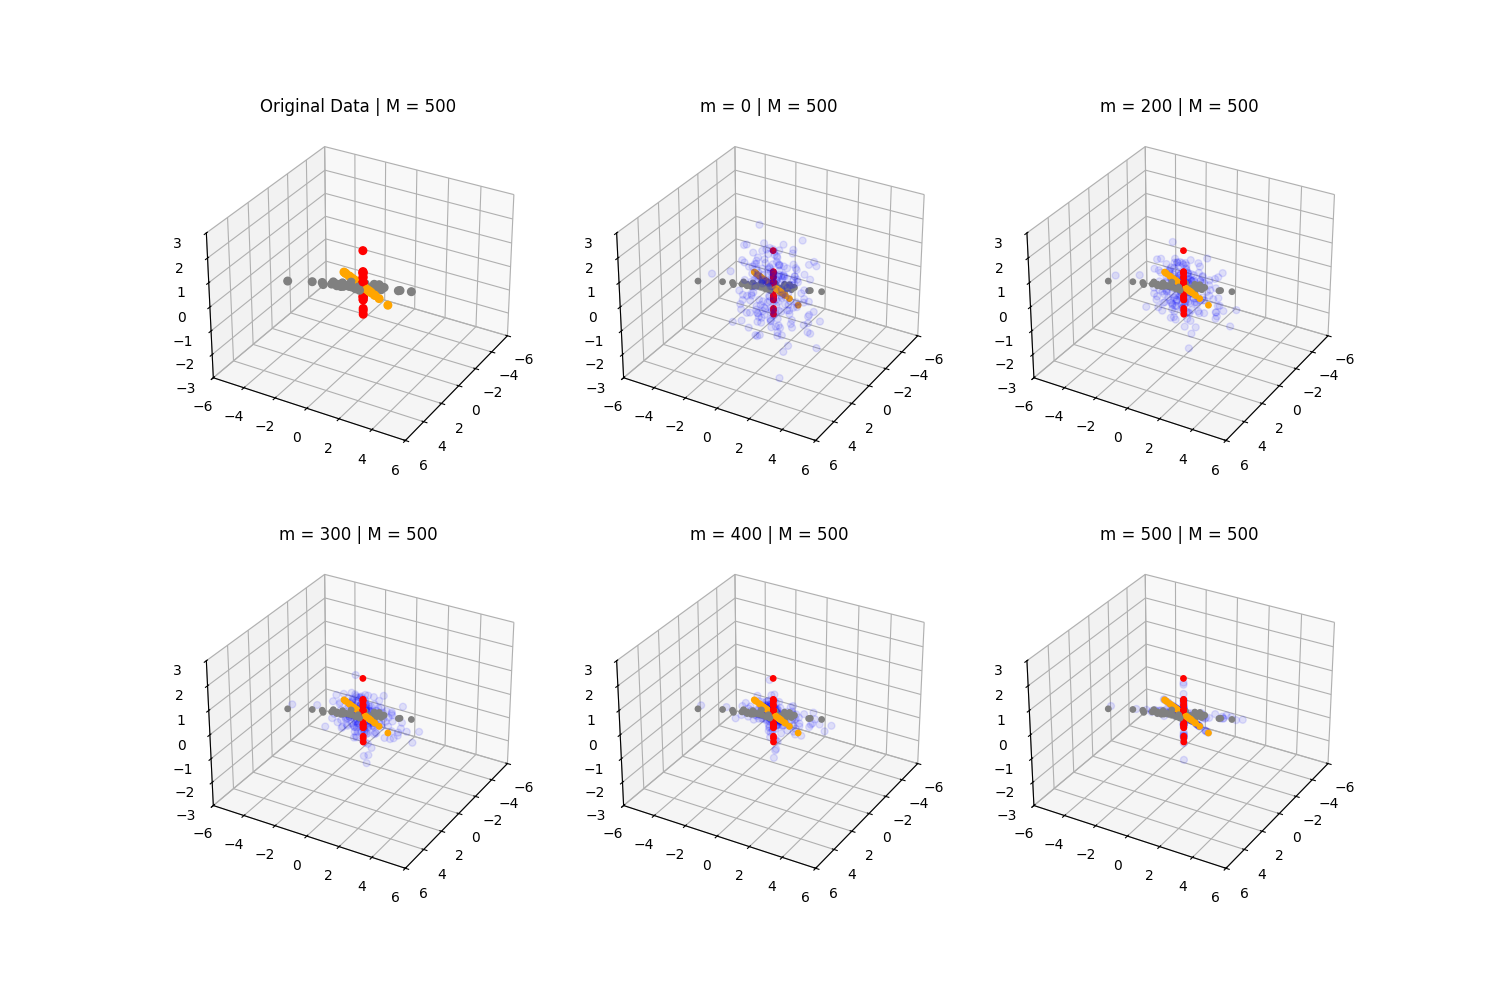
\includegraphics[width=\textwidth]{\toplevelprefix/chapters/chapter3/figs/gaussian_mixture_denoising.png}
% 	\caption{\textbf{Denoising to sample from a mixture of low-rank Gaussians.} \textit{Top left:} We start with three Gaussians, colored gray, orange, and red, supported on a \(2\)-d subspace and two \(1\)-d subspaces respectively in \(\R^{3}\). \textit{Top middle:} We begin the (variance-preserving) denoising process \eqref{eq:denoising_ve_iter} by sampling some noise from \(\dNorm(\vzero, \vI)\). \textit{Top right:} After \(\ell = 200\) iterations, the current iterate \(\tilde{\vx}_{t_{\ell}}\)  starts to develop some structure aligned with the true distribution. \textit{Bottom left, bottom middle:} The same figure with some more denoising iterations, showing that the sampled data structure increases further, aligning more with the true data distribution. \textit{Bottom right:} The output of the sampling procedure, which is distributed very similarly to the original dataset. \yima{Can we make distributions in these plots larger?}}
% 	\label{fig:denoising-twolines-oneplane}
% \end{figure}



% \subsubsection{Parameterizing the Denoiser}

% The sampling error in \Cref{eq:diffusion_sampling_error} is proportional to the average error of the denoiser used for sampling. Usually in practice (for example, when sampling images) we do not know how to specify the denoiser to achieve the minimum possible error. Thus, we parameterize it by using neural networks. Here, we will briefly talk about what our existing theory tells us is a reasonable architecture for such neural networks. For this, we will examine \textit{two} special cases of the Gaussian mixture model denoiser discussed in \Cref{example:gmm_denoising}, since any distribution (of high or low dimension) can be well-approximated by a Gaussian mixture model.

% First, let us attempt to model high-dimensional data with low-dimensional structure by considering \(\vx\) as distributed as an equiprobable mixture of  \(K\) \textit{low-rank} Gaussians, i.e., \(\vx \sim \frac{1}{K}\sum_{k = 1}^{K}\dNorm(\vzero, \vU_{k}\vU_{k}^{\top})\) where \(\vU_{k} \in \R^{D \times P}\) where \(P \ll D\). In particular, suppose that \(\vU_{k} \in \O(D, P)\) is orthogonal, i.e., \(\vU_{k}^{\top}\vU_{k} = \vI\). In this case, the (Bayes) optimal denoiser is
% \begin{equation}
% 	\bar{\vx}^{\ast}(t, \vx_{t}) = \sum_{k = 1}^{K}\frac{\phi(\vx_{t} \mid \vzero, \alpha_{t}^{2}\vU_{k}\vU_{k}^{\top} + \sigma_{t}^{2}\vI)}{\sum_{i = 1}^{K}\phi(\vx_{t} \mid \vzero, \alpha_{t}^{2}\vU_{i}\vU_{i}^{\top} + \sigma_{t}^{2}\vI)}\bp{\alpha_{t}\vU_{k}\vU_{k}^{\top}(\alpha_{t}^{2}\vU_{k}\vU_{k}^{\top} + \sigma_{t}^{2}\vI)^{-1}\vx_{t}}.
% \end{equation}
% To simplify the expression, we can use the Sherman-Morrison-Woodbury identity, namely
% \begin{equation}
% 	(\vA + \vU\vC\vV)^{-1} = \vA^{-1} - \vA^{-1}\vU(\vC^{-1} + \vV\vA^{-1}\vU)^{-1}\vV\vA^{-1}
% \end{equation}
% (for all matrices where the given inverses are well-defined), with \(\vA = \sigma_{t}^{2}\vI\), \(\vU = \vU_{k}\), \(\vV = \vU_{k}^{\top}\), and \(\vC = \alpha_{t}^{2}\vI\), and we obtain
% \begin{align}
% 	(\alpha_{t}^{2}\vU_{k}\vU_{k}^{\top} + \sigma_{t}^{2}\vI)^{-1}
% 	 & = \bp{\frac{1}{\sigma_{t}^{2}}\vI - \frac{1}{\sigma_{t}^{4}}\vU_{k}\bp{\frac{1}{\alpha_{t}^{2}}\vI + \frac{1}{\sigma_{t}^{2}}\vU_{k}^{\top}\vU_{k}}^{-1}\vU_{k}^{\top}} \\
% 	 & = \bp{\frac{1}{\sigma_{t}^{2}}\vI - \frac{1}{\sigma_{t}^{4}}\bp{\frac{1}{\alpha_{t}^{2}} + \frac{1}{\sigma_{t}^{2}}}^{-1}\vU_{k}\vU_{k}^{\top}}                         \\
% 	 & = \frac{1}{\sigma_{t}^{2}}\bp{\vI - \frac{1}{\sigma_{t}^{2}(\frac{1}{\alpha_{t}^{2}} + \frac{1}{\sigma_{t}^{2}})}\vU_{k}\vU_{k}^{\top}}                                 \\
% 	 & = \frac{1}{\sigma_{t}^{2}}\bp{\vI - \frac{1}{1 + (\sigma_{t}/\alpha_{t})^{2}}\vU_{k}\vU_{k}^{\top}}.
% \end{align}
% Since the \(\vU_{k}\)'s are all orthogonal, \(\det(\alpha_{t}^{2}\vU_{k}\vU_{k}^{\top} + \sigma_{t}^{2}\vI)\) are all the same, so
% \begin{align}
% 	\frac{\phi(\vx_{t} \mid \vzero, \alpha_{t}^{2}\vU_{k}\vU_{k}^{\top} + \sigma_{t}^{2}\vI)}{\sum_{i = 1}^{K}\phi(\vx_{t} \mid \vzero, \alpha_{t}^{2}\vU_{i}\vU_{i}^{\top} + \sigma_{t}^{2}\vI)}
% 	 & = \frac{\exp\rp{-\vx_{t}^{\top}(\vI - \frac{1}{1 + (\sigma_{t}/\alpha_{t})^{2}}\vU_{k}\vU_{k}^{\top})\vx_{t}/(2\sigma_{t}^{2})}}{\sum_{i = 1}^{K}\exp\rp{-\vx_{t}^{\top}(\vI - \frac{1}{1 + (\sigma_{t}/\alpha_{t})^{2}}\vU_{i}\vU_{i}^{\top})\vx_{t}/(2\sigma_{t}^{2})}}                                                                                   \\
% 	 & = \frac{\exp\rp{-\frac{1}{2\sigma_{t}^{2}}\vx_{t}^{\top}\vx_{t} + \frac{1}{2\sigma_{t}^{2}[1 + (\sigma_{t}/\alpha_{t})^{2}]}\vx_{t}^{\top}\vU_{k}\vU_{k}^{\top}\vx_{t}}}{\sum_{i = 1}^{K}\exp\rp{-\frac{1}{2\sigma_{t}^{2}}\vx_{t}^{\top}\vx_{t} + \frac{1}{2\sigma_{t}^{2}[1 + (\sigma_{t}/\alpha_{t})^{2}]}\vx_{t}^{\top}\vU_{i}\vU_{i}^{\top}\vx_{t}}}   \\
% 	 & = \frac{\exp\rp{-\frac{1}{2\sigma_{t}^{2}}\norm{\vx_{t}}_{2}^{2} + \frac{1}{2\sigma_{t}^{2}[1 + (\sigma_{t}/\alpha_{t})^{2}]}\norm{\vU_{k}^{\top}\vx_{t}}_{2}^{2}}}{\sum_{i = 1}^{K}\exp\rp{-\frac{1}{2\sigma_{t}^{2}}\norm{\vx_{t}}_{2}^{2} + \frac{1}{2\sigma_{t}^{2}[1 + (\sigma_{t}/\alpha_{t})^{2}]}\norm{\vU_{i}^{\top}\vx_{t}}_{2}^{2}}}             \\
% 	 & = \frac{\exp\rp{-\frac{1}{2\sigma_{t}^{2}}\norm{\vx_{t}}_{2}^{2}}\exp\rp{\frac{1}{2\sigma_{t}^{2}[1 + (\sigma_{t}/\alpha_{t})^{2}]}\norm{\vU_{k}^{\top}\vx_{t}}_{2}^{2}}}{\sum_{i = 1}^{K}\exp\rp{-\frac{1}{2\sigma_{t}^{2}}\norm{\vx_{t}}_{2}^{2}}\exp\rp{\frac{1}{2\sigma_{t}^{2}[1 + (\sigma_{t}/\alpha_{t})^{2}]}\norm{\vU_{i}^{\top}\vx_{t}}_{2}^{2}}} \\
% 	 & = \frac{\exp\rp{\frac{1}{2\sigma_{t}^{2}[1 + (\sigma_{t}/\alpha_{t})^{2}]}\norm{\vU_{k}^{\top}\vx_{t}}_{2}^{2}}}{\sum_{i = 1}^{K}\exp\rp{\frac{1}{2\sigma_{t}^{2}[1 + (\sigma_{t}/\alpha_{t})^{2}]}\norm{\vU_{i}^{\top}\vx_{t}}_{2}^{2}}}.
% \end{align}
% Also, each component denoiser becomes
% \begin{align}
% 	\alpha_{t}\vU_{k}\vU_{k}^{\top}(\alpha_{t}^{2}\vU_{k}\vU_{k}^{\top}(\alpha_{t}^{2}\vU_{k}\vU_{k}^{\top} + \sigma_{t}^{2}\vI)^{-1}\vx_{t})
% 	 & = \alpha_{t}\vU_{k}\vU_{k}^{\top}\cdot\frac{1}{\sigma_{t}^{2}}\bp{\vI - \frac{1}{1 + (\sigma_{t}/\alpha_{t})^{2}}\vU_{k}\vU_{k}^{\top}}\vx_{t} \\
% 	 & = \frac{\alpha_{t}}{\sigma_{t}^{2}}\bp{1 - \frac{1}{1 + (\sigma_{t}/\alpha_{t})^{2}}}\vU_{k}\vU_{k}^{\top}\vx_{t}                              \\
% 	 & = \frac{\alpha_{t}}{\sigma_{t}^{2}}\cdot\frac{(\sigma_{t}/\alpha_{t})^{2}}{1 + (\sigma_{t}/\alpha_{t})^{2}}\cdot \vU_{k}\vU_{k}^{\top}\vx_{t}  \\
% 	 & = \frac{1}{\alpha_{t}[1 + (\sigma_{t}/\alpha_{t})^{2}]}\vU_{k}\vU_{k}^{\top}\vx_{t}.
% \end{align}
% Putting this together,
% \begin{equation}\label{eq:lowrank_gmm_denoiser}
% 	\bar{\vx}^{\ast}(t, \vx_{t}) = \frac{1}{\alpha_{t}[1 + (\sigma_{t}/\alpha_{t})^{2}]}\sum_{k = 1}^{K}\frac{\exp\rp{\frac{1}{2\sigma_{t}^{2}[1 + (\sigma_{t}/\alpha_{t})^{2}]}\norm{\vU_{k}^{\top}\vx_{t}}_{2}^{2}}}{\sum_{i = 1}^{K}\exp\rp{\frac{1}{2\sigma_{t}^{2}[1 + (\sigma_{t}/\alpha_{t})^{2}]}\norm{\vU_{i}^{\top}\vx_{t}}_{2}^{2}}}\vU_{k}\vU_{k}^{\top}\vx_{t}.
% \end{equation}

% This is a softmax which weights each component denoiser based on the projection magnitude of \(\vx_{t}\) onto \(\vU_{k}\), similar to the attention mechanism in transformers. As we will see in \Cref{ch:representation}, this resemblance is not a mere coincidence: denoising against mixtures of Gaussians is very closely related to compression mechanisms and ultimately the attention mechanism in transformer networks.

% So, this theory seems to suggest (loosely speaking) that in practice, using a transformer-like network is reasonable for denoising. This is reasonable, but what is the problem with using any old neural network (such as a multi-layer perceptron (MLP)) and just trying to scale it up to infinity? To observe the problem with this, let us look at another special case of the Gaussian mixture model. Namely, the \textit{empirical distribution} is also an instance of a degenerate Gaussian mixture model, with \(K = N\) components \(\dNorm(\vx_{i}, \vzero)\) sampled with equal probability \(\pi_{i} = \frac{1}{N}\). In this case the Bayes optimal denoiser is
% \begin{equation}\label{eq:memorizing_denoiser}
% 	\bar{\vx}^{\star}(t, \vx_{t}) = \sum_{i = 1}^{N}\frac{e^{-\|\vx_{t} - \alpha_{t}\vx_{i}\|_{2}^{2}/(2\sigma_{t}^{2})}}{\sum_{j = 1}^{N}e^{-\|\vx_{t} - \alpha_{t}\vx_{j}\|_{2}^{2}/(2\sigma_{t}^{2})}}\vx_{i}.
% \end{equation}
% This is a convex combination of the data \(\vx_{i}\), and the coefficients get ``sharper'' (i.e., closer to \(0\) or \(1\)) as \(t \to 0\). Notice that this denoiser \textit{optimally solves} the denoising optimization problem \eqref{eq:denoising_loss_all_t} when we compute the loss based on drawing \(\vx\) uniformly at random from a fixed finite dataset \(\vX = \{\vx_{i}\}_{i = 1}^{N}\). This is the realistic setting. Thus, if the function family \(\cF\) we use in practice is large enough such that optimal denoisers of the above form \eqref{eq:memorizing_denoiser} may be approximated, then the learned denoiser may do just that. Then, our iterative denoising algorithm will sample exactly from the empirical distribution, re-generating samples in the training data. This is a bad sampler, not really more interesting than a database of all samples, and so it is important to understand how to avoid this in practice. The key is to come up with a function family which can well-approximate the true denoiser (say corresponding to a low-rank distribution as in \eqref{eq:lowrank_gmm_denoiser}) but not the empirical Bayesian denoiser as in \eqref{eq:memorizing_denoiser}. Some work has explored this fine line and why modern diffusion models, which use transformer- and convolutional-based network architectures, can memorize and generalize in different regimes \citep{kamb2024analytic,niedoba2024towards}.

% At a high level, a denoiser which memorizes all the training points, as in \eqref{eq:memorizing_denoiser}, corresponds to a parametric model of the distribution which has absolutely minimal coding rate, and achieves this by just coding every sample separately. We will discuss this problem (and seeming paradox with our initial desiderata at the end of \Cref{sub:min_entropy}) from the perspective of information theory in the next Section.

% \subsubsection{Learning a Denoiser vs.~Learning a Density}

% So far we have talked about learning the distribution by training a denoiser. This uses a particular definition of ``learning''. However, in the literature, it is often the case that ``learning the distribution'' corresponds to learning the probability measure or density of the data distribution. We now discuss a direct connection between our denoising formulation and a way to learn the distribution in this density-centric paradigm. The connection follows from \textit{Tweedie's formula} \cite{Robbins1956AnEB}, which we repeat below.

% \begin{theorem}[Tweedie's Formula]\label{thm:tweedie}
% 	Let the notation used in \eqref{eq:gen_additive_gaussian_noise_model} prevail. Then
% 	\begin{equation}
% 		\Ex[\vx \mid \vx_{t}] = \frac{1}{\alpha_{t}}\bp{\vx_{t} + \sigma_{t}^{2}\nabla \log p_{t}(\vx_{t})},
% 	\end{equation}
% 	where \(p_{t}\) is the density of \(\vx_{t}\).
% \end{theorem}
% \begin{proof}
% 	For the sake of this proof, suppose that \(\vx\) has probability density function \(p\) (though the result is true even in the case \(\vx\) does not have a density). Then, note that \(p_{t}\) can be factored into
% 	\begin{equation}
% 		p_{t}(\vx_{t}) = \int_{\R^{D}}p(\vx)p_{t \mid 0}(\vx_{t} \mid \vx)\odif{\vx},
% 	\end{equation}
% 	where \(p_{t \mid 0}\) is the probability density of \(\vx_{t}\) given an observation of \(\vx = \vx_{0}\). Define \(p_{0 \mid t}\) correspondingly. Now, we know from the noise model that
% 	\begin{equation}
% 		p_{t \mid 0}(\vx_{t} \mid \vx) = \phi(\vx_{t} \mid \alpha_{t}\vx, \sigma_{t}^{2}\vI),
% 	\end{equation}
% 	where \(\phi(\vmu, \vSigma)\) is the density of the normal distribution with mean \(\vmu\) and covariance \(\vSigma\). Then
% 	\begin{align}
% 		\nabla \log p_{t}(\vx_{t})
% 		 & = \frac{1}{p_{t}(\vx_{t})}\nabla p_{t}(\vx_{t})                                                                                                                                                      \\
% 		 & = \frac{1}{p_{t}(\vx_{t})}\nabla_{\vx_{t}}\int_{\R^{D}}p(\vx)\phi(\vx_{t} \mid \alpha_{t}\vx, \sigma_{t}^{2}\vI)\odif{\vx}                                                                           \\
% 		 & = \frac{1}{p_{t}(\vx_{t})}\int_{\R^{D}}p(\vx)\bs{\nabla_{\vxi}\phi(\vx_{t} \mid \alpha_{t}\vx, \sigma_{t}^{2}\vI)}\odif{\vx}                                                                         \\
% 		 & = \frac{1}{p_{t}(\vx_{t})}\int_{\R^{D}}p(\vx)\bs{\phi(\vx_{t} \mid \alpha_{t}\vx, \sigma_{t}^{2}\vI)\cdot \frac{\alpha_{t}\vx - \vx_{t}}{\sigma_{t}^{2}}}\odif{\vx}                                  \\
% 		 & = \frac{1}{\sigma_{t}^{2}p_{t}(\vx_{t})}\int_{\R^{D}}p(\vx)\phi(\vx_{t} \mid \alpha_{t}\vx, \sigma_{t}^{2}\vI)[\alpha_{t}\vx - \vx_{t}]\odif{\vx}                                                    \\
% 		 & = \frac{\alpha_{t}}{\sigma_{t}^{2}p_{t}(\vx_{t})}\int_{\R^{D}}p(\vx)\phi(\vx_{t} \mid \alpha_{t}\vx, \sigma_{t}^{2}\vI)\vx\odif{\vx}                                                                 \\
% 		 & \qquad - \frac{1}{\sigma_{t}^{2}p_{t}(\vx_{t})}\vx_{t}\int_{\R^{D}}p(\vx)\phi(\vx_{t} \mid \alpha_{t}\vx, \sigma_{t}^{2}\vI)\odif{\vx}                                                               \\
% 		 & = \frac{\alpha_{t}}{\sigma_{t}^{2}p_{t}(\vx_{t})}\int_{\R^{D}}p(\vx)\phi(\vx_{t} \mid \alpha_{t}\vx, \sigma_{t}^{2}\vI)\vx\odif{\vx} - \frac{1}{\sigma_{t}^{2}p_{t}(\vx_{t})}\vx_{t} p_{t}(\vx_{t}), \\
% 		 & = \frac{\alpha_{t}}{\sigma_{t}^{2}p_{t}(\vx_{t})}\int_{\R^{D}}p(\vx)\phi(\vx_{t} \mid \alpha_{t}\vx, \sigma_{t}^{2}\vI)\vx\odif{\vx} - \frac{1}{\sigma_{t}^{2}}\vx_{t}.
% 	\end{align}
% 	Let us consider the remaining integral. Remember that \(\phi(\vx_{t} \mid \alpha_{t}\vx, \sigma_{t}^{2}\vI) = p_{t \mid 0}(\vx_{t} \mid \vx)\). By Bayes' theorem, we write
% 	\begin{equation}
% 		p(\vx)\phi(\vx_{t} \mid \alpha_{t}\vx, \sigma_{t}^{2}\vI) = p(\vx)p_{t \mid 0}(\vx_{t} \mid \vx) = p_{t}(\vx_{t})p_{0 \mid t}(\vx \mid \vx_{t}),
% 	\end{equation}
% 	which allows us to rewrite the integrand in more favorable terms, overall obtaining
% 	\begin{align}
% 		\nabla \log p_{t}(\vx_{t})
% 		 & = \frac{\alpha_{t}}{\sigma_{t}^{2}p_{t}(\vx_{t})}\int_{\R^{D}}p(\vx)\phi(\vx_{t} \mid \alpha_{t}\vx, \sigma_{t}^{2}\vI)\vx\odif{\vx} - \frac{1}{\sigma_{t}^{2}}\vx_{t} \\
% 		 & = \frac{\alpha_{t}}{\sigma_{t}^{2}p_{t}(\vx_{t})}\int_{\R^{D}}p_{t}(\vx_{t})p_{0 \mid t}(\vx \mid \vx_{t})\vx\odif{\vx} - \frac{1}{\sigma_{t}^{2}}\vx_{t}              \\
% 		 & = \frac{\alpha_{t}}{\sigma_{t}^{2}}\int_{\R^{D}}p_{0 \mid t}(\vx \mid \vx_{t})\vx\odif{\vx} - \frac{1}{\sigma_{t}^{2}}\vx_{t}                                          \\
% 		 & = \frac{\alpha_{t}}{\sigma_{t}^{2}}\Ex[\vx \mid \vx_{t}] - \frac{1}{\sigma_{t}^{2}}\vx_{t}.
% 	\end{align}
% 	Rearranging proves the theorem.
% \end{proof}

% This result forms a connection between estimating the conditional expectation \(\Ex[\vx \mid \vx_{t}]\), i.e., learning a denoiser \(\bar{\vx}(t, \cdot)\), and estimating the (gradients of the log-density of) the data distribution \(\nabla \log p_{t}\), also known as the \textit{(Hyv{\"a}rinen) score \cite{hyvarinen05a}}. We already have a recipe for estimating \(\Ex[\vx \mid \vx_{t}]\) (i.e., \Cref{alg:learning_denoiser}), and we can thus convert this estimate into an estimate for \(\nabla \log p_{t}\). As we have seen in \Cref{ch:intro}, \Cref{fig:score-function} illustrates the geometric intuition of the score in the case of a 1D distribution. We have already discussed how to use estimates for \(\Ex[\vx \mid \vx_{t}]\) to iteratively transform high-entropy distributions towards the (low-dimensional) data distribution; we can do the same with \(\nabla \log p_{t}\) using Tweedie's formula in \Cref{thm:tweedie}. In this sense, by learning a denoiser using a parametric function family \(\cF = \{\bar{\vx}_{\theta} \colon \theta \in \Theta\}\), we learn a parametric encoding of the distribution\, as desired in accordance with the stated goals in \Cref{sub:min_entropy}.

% \subsubsection{Recap}

% Let us recap what we have covered so far. We have discussed how to fit a \textit{denoiser} \(\bar{\vx}\) from a parametric function class \(\cF\) using finite samples. We have shown that this denoiser encodes a distribution in two ways: first, we can use it to gradually transform a pure noise (high-entropy) distribution towards the learned distribution via \textit{iterative denoising}, and second, it is equivalent to the target distribution's (gradient of log) density via Tweedie's formula (\Cref{thm:tweedie}). This iterative denoising process is thus a realization of \textit{both} ways of learning or pursuing a distribution laid out at the end of \Cref{sub:min_entropy}.

% Nevertheless, in this methodology the encoding of the distribution is more or less implicit. In the sequel, we discuss a framework for making our model of the distribution more explicit and computationally accessible.


% \begin{exercise}\label{exercise:noise_prediction}
% 	In practice, a common technique is to not predict \(\vx\) but rather predict \(\vg\) --- this is fittingly called \textit{noise prediction}. Analogous results and algorithms can be derived for noise prediction. In this exercise, please derive a training procedure for noise prediction, a sampling procedure which uses noise prediction, find the error rate in \Cref{thm:diffusion_sampler_convergence} in terms of noise prediction, and modify \Cref{thm:tweedie} to express \(\Ex[\vg \mid \vx_{t}]\) in terms of \(\nabla \log p_{t}\).

% 	\textit{PS:} Another technique is to predict \(\odv*{\vx_{t}}{t}\) instead of \(\vx\) --- this is called \textit{velocity prediction} or \textit{\(v\)-prediction}. Surprisingly, each of velocity prediction, noise prediction, and denoising are completely equivalent tasks under the additive noise model \eqref{eq:gen_additive_gaussian_noise_model}. You can repeat the same exercise above for \(v\)-prediction.
% \end{exercise}

% \begin{example}\label{exercise:}
% 	Reproduce \Cref{fig:denoising-twolines-oneplane}.

% 	\textit{Hint:} You may want to set \(t_{L + 1} < 1\), so that \(\sigma_{t_{L + 1}} \neq 0\) (avoiding divide-by-\(0\) issues).
% \end{example}


% Suppose that \(\vz_{\sigma}\) is a perturbation of \(\vz_{o}\) by additive Gaussian noise, i.e.,
% \begin{equation}\label{eq:additive_gaussian_noise_model}
%     \vz_{\sigma} = \vz_{o} + \sigma \vg, \qquad \vg \sim \dNorm(\vzero, \vI).
% \end{equation}
% The following theorem shows that, by adding Gaussian noise, the differential entropy of the
% resulting distribution indeed increases. \sdb{TODO: hammer transitions a bit.
% the resolution to the negative infinity diffent paradox is the lossy coding/rate
% distortion scheme later... think about the transition. also cf the modern
% practice of VQ-VAE. for this part, it's okay if this is the ``how to do it in
% the very clean setting'' (practical later via discretization), as long as the
% transition/context is good}
% \begin{theorem}[Diffusion and Entropy]\label{thm:diffusion-and-entropy}
%     Suppose that \(\vz_{o} \in \R^{d}\) is a random variable with a well-defined
%     differential entropy $h(\vz_o)$, %
%     %with \(\Ex\norm{\vz_{o}}_{2}^{2} < \infty\),
%     \(\vg \sim \dNorm(\vzero, \vI)\) is a standard Gaussian random variable which is independent of \(\vz_{o}\), \(\sigma > 0\) is a positive real number, and \(\vz_{\sigma} = \vz_{o} + \sigma \vg\). Then \(h(\vz_{\sigma}) > h(\vz_{o})\).
% \end{theorem}
% The justification is concise but requires somewhat sophisticated mathematics that is beyond the scope of this book. We have left the details in Appendix \ref{app:diffusion-denoising}.
% The proof demonstrates a rigorous way to establish, by a limiting argument, that
% $h(\vz_o) = -\infty$ for large classes of degenerate distributions, as we
% claimed earlier, and therefore the same increase of entropy asserted in
% \Cref{thm:diffusion-and-entropy} applies to this important class of
% distributions.
% % \yima{probably state as a theorem or proposition.}

% The inverse operation to removing isotropic Gaussian noise is known as \textit{denoising}. It is a classical and well-studied topic in signal processing and system theory, such as the Wiener filter and the Kalman filter. The several problems discussed in Chapter \ref{ch:classic} such as PCA, ICA, and Dictionary Learning, are specific instances of the denoising problem. Specifically, the denoising problem can be formulated as attempting to learn a function \(\vmu_{\sigma} \colon \R^{d} \to \R^{d}\) which solves the maximum likelihood estimation problem to estimate \(\vz_{o}\) from \(\vmu_{\sigma}\):
% \begin{equation}\label{eq:denoiser_maximum_likelihood}
%     \vmu_{\sigma} \in \argmax_{\substack{f \colon \R^{d} \to \R^{d},\
%     %\\%f\ \text{measurable} \\
%     \Ex\norm{f(\vz_{\sigma})}_{2}^{2} < \infty}}\Ex \log p_{\sigma \mid o}(f(\vz_{\sigma})),
% \end{equation}
% In particular, the denoiser \(\vmu_{\sigma}\) finds the value of the true data which makes the noisy observations most likely. It is easy to show that finding the function \(\vmu_{\sigma}\), with the Gaussian noise model \eqref{eq:additive_gaussian_noise_model}, is equivalent to solving the problem
% %\footnote{If you aren't sure what \textit{measurable} means, don't worry about it; it's merely a technical condition, which holds for any function you can write down. Its exact definition can be looked up in any graduate-level real analysis or probability textbook.}
% \begin{equation}\label{eq:denoiser_conditional_expectation}
%     \vmu_{\sigma} \in \argmin_{\substack{f \colon \R^{d} \to \R^{d},\ %\\% \text{\(f\) measurable} \\
%     \Ex\norm{f(\vz_{\sigma})}_{2}^{2} < \infty}}\Ex\norm{\vz_{o} - f(\vz_{\sigma})}_{2}^{2}.
% \end{equation}
% Namely, for some function class \(\cF\) containing some potential denoising functions, say a family of neural networks with the same architecture and different weights, we can solve the denoising problem
% \begin{equation}\label{eq:denoiser_learning_problem}
%     f^{\ast} \in \argmin_{f \in \cF}\Ex\norm{\vz_{o} - f(\vz_{\sigma})}_{2}^{2}.
% \end{equation}
% % It turns out that solving the minimization problem in \eqref{eq:denoiser_conditional_expectation} is \textit{much} more computationally tractable than solving the maximum likelihood problem \eqref{eq:denoiser_maximum_likelihood}.
% To solve this problem, we use the following algorithm outlined \Cref{alg:denoiser}.
% \begin{algorithm}
%     \caption{Learning a Denoiser}
%         \label{alg:denoiser}
%     \begin{algorithmic}[1]
%         \Require{An optimization algorithm, a parametric function class \(\cF = \{f_{\vtheta} \colon \vtheta \in \vTheta\}\), an initial parameter \(\vtheta^{1}\), a noise level \(\sigma > 0\), and data \(\vz_{o}^{1}, \dots, \vz_{o}^{N} \simiid \vz_{o}\).}
%         \Ensure{A denoiser \(f_{\vtheta^{\ast}}\).}

%         \Procedure{TrainDenoiser}{\texttt{OptUpdate}, $\cF$, $\vtheta^{1}$, $\sigma$, $\{\vz_{o}^{i}\}_{i = 1}^{N}$}
%         \For{each iteration \(j \in [M]\)}
%             \For{each sample \(i \in [N]\)}
%                 \State{\(\vg^{i, j} \gets \) sample from \(\dNorm(\vzero, \vI)\)} \Comment{\(\vg^{i, j}\) is independent of everything}
%                 \State{\(\vz_{\sigma}^{ij} \gets \displaystyle \vz_{o}^{i} + \sigma \vg^{i, j}\)}
%             \EndFor
%             \State{\(\ell^{j} \gets \displaystyle\frac{1}{N}\sum_{i = 1}^{N}\norm{\vz_{o}^{i} - f_{\vtheta^{j}}(\vz_{\sigma, j}^{i})}_{2}^{2}\)} \Comment{\(\ell^{j}\) is estimate of ``true'' denoising loss}
%             \State{\(\vtheta^{j + 1} \gets \displaystyle \texttt{OptUpdate}(\vtheta^{j}; \ell^{j})\)} \Comment{Update \(\vtheta^{j + 1}\) via optimization, i.e., \(\vtheta^{j + 1} \gets \vtheta^{j} - \alpha \nabla_{\vtheta}\ell^{j}\) for SGD.}
%             \EndFor
%         \State{\Return{\(f_{\vtheta^{M+1}}\)}}
%         \EndProcedure
%     \end{algorithmic}
% \end{algorithm}

% The only thing that needs to be specified in the algorithm is the form of the function class $\mathcal{F}$. For special classes of distributions, such as Gaussian, the function form can be explicitly derived.

% \begin{example}[Denoising Gaussian noise from a Gaussian]\label{example:gaussian_denoising}
%     Consider the case where \(\vz_{o}\) is a Gaussian, say \(\vz_{o} \sim \dNorm(\vu, \vSigma)\). Then \(\vz_{\sigma} \sim \dNorm(\vu, \vSigma + \sigma^{2}\vI)\) where \(\vSigma\) is nonsingular. Then \(\vz_{o}\) and \(\vz_{\sigma}\) are jointly Gaussian, i.e.,
%     \begin{equation}
%         \mat{\vz_{o} \\ \vz_{\sigma}} \sim \dNorm\rp{\mat{\vu \\ \vu}, \mat{\vSigma & \vSigma \\ \vSigma & \vSigma + \sigma^{2}\vI}},
%     \end{equation}
%     and the posterior distribution of \(\vz_{o}\) given \(\vz_{\sigma}\) is (famously)
%     \begin{equation}
%         \vz_{o} \mid \vz_{\sigma} \sim \dNorm(\vu + \vSigma(\vSigma + \sigma^{2}\vI)^{-1}(\vz_{\sigma} - \vu), \vSigma - \vSigma (\vSigma + \sigma^{2}\vI)^{-1}\vSigma).
%     \end{equation}
%     Thus we have
%     \begin{equation}\label{eq:gaussian_denoiser}
%         \vmu_{\sigma}(\vxi) = \vu + \vSigma(\vSigma + \sigma^{2}\vI)^{-1}(\vxi - \vu),
%     \end{equation}
%     which provides an answer for both denoising problems. Letting \(\vSigma = \vV\vLambda\vV^{\top}\) where \(\vLambda = \diag(\lambda_{1}, \dots, \lambda_{d})\), we have
%     \begin{equation}
%         \vmu_{\sigma}(\vxi) = \vu + \vV\diag\mat{\lambda_{1}/(\lambda_{1} + \sigma^{2}) & & \\ & \ddots & \\ & & \lambda_{d}/(\lambda_{d} + \sigma^{2})}\vV^{\top}(\vxi - \vu).
%     \end{equation}
%     which shows that as \(\sigma\) grows, the denoiser collapses the residual \(\vxi - \vu\) to \(0\) fastest in the directions where the eigenvalues of \(\vSigma\) are smallest. Also, if we are trying to learn a Gaussian (for instance), we can parameterize the denoiser by the mean \(\vu\) and covariance \(\vSigma\), so that \(\vtheta = (\vu, \vSigma)\), and consider denoisers of the functional form \eqref{eq:gaussian_denoiser}.
% \end{example}

% Using the definition in \eqref{eq:denoiser_conditional_expectation}, one can show that \(\vmu_{\sigma}\) is the conditional expectation of \(\vz_{o}\) given \(\vz_{\sigma}\),\footnote{We leave this as an exercise for the reader to verify.} i.e.,
% \begin{equation}
%     \vmu_{\sigma}(\vxi) = \Ex[\vz_{o} \mid \vz_{\sigma} = \vxi].
% \end{equation}
% One may use this to show that denoising reduces the entropy $h(\vz)$, as desired.
% \begin{theorem}[Denoising and Entropy]\label{thm:conditioning_reduces_entropy}
%     Suppose that \(\vz_{o} \in \R^{d}\) is a random variable,
%     %with \(\Ex\norm{\vz_{o}}_{2}^{2} < \infty\),
%     \(\vg \sim \dNorm(\vzero, \vI)\) is a standard Gaussian random variable
%     which is independent of \(\vz_{o}\), \(\sigma > 0\) is a positive real
%     number, \(\vz_{\sigma} = \vz_{o} + \sigma \vg\), and \(\vmu_{\sigma}(\vz)
%     = \Ex[\vz_{o} \mid \vz_{\sigma} = \vz]\). Then under certain regularity
%     conditions on $\vz_o$ (detailed in \Cref{app:diffusion-denoising}), it holds
%     that \(h(\vmu_{\sigma}(\vz_{\sigma})) < h(\vz_{\sigma})\).
% \end{theorem}
% The proof is slightly technical and deferred to
% \Cref{app:diffusion-denoising}. Regarding the necessary regularity conditions on
% $\vz_o$, it suffices to assume that $\vz_o$ is any random variable with an arbitrarily small amount of independent Gaussian noise added to it. In the sequel, we will use \textit{iterative denoising} to lower the entropy of
% a high-entropy distribution until it reaches the data distribution, realizing
% the second approach to pursuing a distribution discussed at the end of \Cref{sub:min_entropy}: this makes \Cref{thm:conditioning_reduces_entropy}
% applicable to stages of the iterative denoising process corresponding to
% removing previously added noise from the data distribution.

% So far we have talked about learning the distribution using a particular definition of ``learning''. However, in the literature, it is often the case that ``learning the distribution'' corresponds to learning the probability measure or density of the data distribution. We now discuss a direct connection between our denoising formulation and a way to learn the distribution in this density-centric paradigm. The connection follows from \textit{Tweedie's formula} \cite{Robbins1956AnEB}, which we repeat below.

% \begin{theorem}[Tweedie's Formula]\label{thm:tweedie}
%     Suppose that \(\vz_{o} \in \R^{d}\) is a random variable with \(\Ex\norm{\vz_{o}}_{2}^{2} < \infty\), \(\vg \sim \dNorm(\vzero, \vI)\) is a standard Gaussian random variable which is independent of \(\vz_{o}\), \(\sigma > 0\) is a positive real number, \(\vz_{\sigma} = \vz_{o} + \sigma \vg\), and \(p_{\sigma}\) is the probability density function of \(\vz_{\sigma}\). Then
%     \begin{equation}
%         \Ex[\vz_{o} \mid \vz_{\sigma} = \vxi] = \vxi + \sigma^{2}\nabla \log p_{\sigma}(\vxi).
%     \end{equation}
% \end{theorem}
% \begin{proof}
%     For the sake of this proof, suppose that \(\vz_{o}\) has probability density function \(p_{o}\) (though the result is true even in the case \(\vz_{o}\) does not have a density). Then, note that \(p_{\sigma}\) can be factored into
%     \begin{equation}
%         p_{\sigma}(\vxi) = \int_{\R^{d}}p_{o}(\vx)p_{\sigma \mid o}(\vxi \mid \vx)\odif{\vx},
%     \end{equation}
%     where \(p_{\sigma \mid o}\) is the probability density of \(\vz_{\sigma}\) given an observation of \(\vz_{o}\). Define \(p_{o \mid \sigma}\) correspondingly. Now, we know from the noise model that
%     \begin{equation}
%         p_{\sigma \mid o}(\vxi \mid \vx) = \phi(\vxi \mid \vx, \sigma^{2}\vI),
%     \end{equation}
%     where \(\phi(\vmu, \vSigma)\) is the density of the normal distribution with mean \(\vmu\) and covariance \(\vSigma\). Then
%     \begin{align}
%         \nabla \log p_{\sigma}(\vxi)
%         &= \frac{1}{p_{\sigma}(\vxi)}\nabla p_{\sigma}(\vxi) \\
%         &= \frac{1}{p_{\sigma}(\vxi)}\nabla_{\vxi}\int_{\R^{d}}p_{o}(\vx)\phi(\vxi \mid \vx, \sigma^{2}\vI)\odif{\vx} \\
%         &= \frac{1}{p_{\sigma}(\vxi)}\int_{\R^{d}}p_{o}(\vx)\bs{\nabla_{\vxi}\phi(\vxi \mid \vx, \sigma^{2}\vI)}\odif{\vx} \\
%         &= \frac{1}{p_{\sigma}(\vxi)}\int_{\R^{d}}p_{o}(\vx)\bs{\phi(\vxi \mid \vx, \sigma^{2}\vI)\frac{\vx - \vxi}{\sigma^{2}}}\odif{\vx} \\
%         &= \frac{1}{\sigma^{2}p_{\sigma}(\vxi)}\int_{\R^{d}}p_{o}(\vx)\phi(\vxi \mid \vx, \sigma^{2}\vI)[\vx - \vxi]\odif{\vx} \\
%         &= \frac{1}{\sigma^{2}p_{\sigma}(\vxi)}\int_{\R^{d}}p_{o}(\vx)\phi(\vxi \mid \vx, \sigma^{2}\vI)\vx\odif{\vx} \\
%         &\qquad - \frac{1}{\sigma^{2}p_{\sigma}(\vxi)}\vxi\int_{\R^{d}}p_{o}(\vx)\phi(\vxi \mid \vx, \sigma^{2}\vI)\odif{\vx} \\
%         &= \frac{1}{\sigma^{2}p_{\sigma}(\vxi)}\int_{\R^{d}}p_{o}(\vx)\phi(\vxi \mid \vx, \sigma^{2}\vI)\vx\odif{\vx} - \frac{1}{\sigma^{2}p_{\sigma}(\vxi)}\vxi p_{\sigma}(\vxi), \\
%         &= \frac{1}{\sigma^{2}p_{\sigma}(\vxi)}\int_{\R^{d}}p_{o}(\vx)\phi(\vxi \mid \vx, \sigma^{2}\vI)\vx\odif{\vx} - \frac{1}{\sigma^{2}}\vxi.
%     \end{align}
%     Let us consider the remaining integral. Remember that \(\phi(\vxi \mid \vx, \sigma^{2}\vI) = p_{\sigma \mid o}(\vxi \mid \vx)\). By Bayes' theorem, we write
%     \begin{equation}
%         p_{o}(\vx)\phi(\vxi \mid \vx, \sigma^{2}\vI) = p_{o}(\vx)p_{\sigma \mid o}(\vxi \mid \vx) = p_{\sigma}(\vxi)p_{o \mid \sigma}(\vx \mid \vxi),
%     \end{equation}
%     which allows us to rewrite the integrand in more favorable terms, overall obtaining
%     \begin{align}
%         \nabla \log p_{\sigma}(\vxi)
%         &= \frac{1}{\sigma^{2}p_{\sigma}(\vxi)}\int_{\R^{d}}p_{o}(\vx)\phi(\vxi \mid \vx, \sigma^{2}\vI)\vx\odif{\vx} - \frac{1}{\sigma^{2}}\vxi \\
%         &= \frac{1}{\sigma^{2}p_{\sigma}(\vxi)}\int_{\R^{d}}p_{\sigma}(\vxi)p_{o \mid \sigma}(\vx \mid \vxi)\vx\odif{\vx} - \frac{1}{\sigma^{2}}\vxi \\
%         &= \frac{1}{\sigma^{2}}\int_{\R^{d}}p_{o \mid \sigma}(\vx \mid \vxi)\vx\odif{\vx} - \frac{1}{\sigma^{2}}\vxi \\
%         &= \frac{1}{\sigma^{2}}\bp{\Ex[\vz_{o} \mid \vz_{\sigma} = \vxi] - \vxi}.
%     \end{align}
%     Rearranging proves the theorem.
% \end{proof}
%\yima{Tweedie's formula for the scalar case... as an example of an exercise.}
%\DP{Exercise \ref{exercise:vp_tweedie_denoising} gives a better exercise about these contents. Scalar Tweedie's formula is not a good question since it just repeats the same calculation as here.}

% This result forms a connection between estimating the conditional expectation \(\Ex[\vz_{o} \mid \vz_{\sigma}]\) and estimating the (gradients of the log-density of) the data distribution \(\nabla \log p_{\sigma}\), also known as the \textit{(Hyv{\"a}rinen) score \cite{hyvarinen05a}}. We already have a recipe for estimating \(\Ex[\vz_{0} \mid \vz_{\sigma}]\), so in turn we have a recipe for estimating \(\nabla \log p_{\sigma}\). As we have seen in Chapter \ref{ch:intro}, Figure \ref{fig:score-function} illustrates the geometric intuition of the score in the case of a 1D distribution. In the sequel, we will discuss how to use our estimates for \(\nabla \log p_{\sigma}\) to iteratively transform high-entropy distributions towards the (low-dimensional) data distribution.

% \yima{I have some concerns with the notation here. A few notations are related but are used without clarifying their relationships:  we use $f_{\bm_{\theta}}$ in Algorithm \ref{alg:denoiser}, but use $\bm{\mu}_\sigma$ in Algorithm \ref{alg:iterative_denoising}... We use the notation $\bm{s}_\sigma$ in Algorithm \ref{alg:iterative_denoising} but never quite explain its relation with the score $\nabla \log p_{\sigma}$. Anyway, currently the presentation is not written for first timers. Even experienced need to sort out or guess the notation...  }

% \yima{How to solve this? Does one need to parameterize $f$? The reader needs to solve this for each $\z_o$?}

%\yima{This paragraph. Please do not make comments as if the reader already knows the answers to the denoising problem. This is a book not a paper. We should directly describe how to solve the denoising problem. Some comments could be made AFTER the facts have been presented.}
%At a very high level, denoising follows the general approach we declared in order to learn a distribution. However, there \textit{also} exist very concrete connections between the conditional expectation, i.e., the optimal denoiser, to (perturbed versions of) the data distribution. These mostly follow from \textit{Tweedie's formula} \DP{cite: Robbins 1957, or before?} \DP{cite: Jong-Chul Ye DPM, which has the most general form of Tweedie's formula that I know} \DP{cite: Druv's MAE paper}, whose simplest form is as follows. Consider the model \eqref{eq:additive_gaussian_noise_model}, let \(p_{\sigma}\) be the probability density of \(\vz_\sigma\), and let \(\vs_{\sigma} \doteq \nabla \log p_{\sigma}\). Then
% \begin{equation}\label{eq:tweedie_simple}
%     \vmu_{\sigma}(\vz) \doteq \Ex[\vz_{o} \mid \vz_{\sigma} = \vz] = \vz + \sigma^{2}\nabla \log p_{\sigma}(\vz) \doteq \vz + \sigma^{2}\vs_{\sigma}(\vz).
% \end{equation}
% Thus, it is equivalent to learn a perturbed version of the data distribution via \(\nabla \log p^{\sigma}\), also called the (Hyvarinen) score \DP{cite: aapo score matching} \DP{cite: sohl-dickstein, ganguli}, and to solve the simple conditional expectation regression problem \eqref{eq:denoiser_learning_problem}, which is much more tractable. \yima{this sentence is very awkward: what are equivalent? which is more tractable? We need to describe exactly how the conditional expectation can be solved and the score function can be represented and estimated, at least for the Gaussian noise case. Describe clearly one way and probably comment on other alterative ways to estimate the score etc. Or leave as exercises.}



% It can be shown that the resulting data distribution following the above denoising (with the score) always has entropy reduced: $$h(\boldsymbol{\mu}_\sigma) < h(\z_\sigma).$$
% Again, see Appendix \ref{app:diffusion-denoising} for the justification. \yima{probably state as a theorem.}

% \subsection{Sampling via Iterative Denoising}

% Previously, we have discussed a recipe for learning a parametric encoding of the data distribution, via fitting a denoiser from a parametric family of functions. We also observed, in \ref{thm:conditioning_reduces_entropy}, that applying the denoiser would reduce the entropy of a noisy distribution. In this section, we will discuss how to carefully use this denoiser to gradually reduce the entropy of a noisy distribution until it reaches the data distribution, thereby \textit{sampling} from the distribution. This procedure, known as \textit{iterative denoising} or \textit{iterative compression}, is a realization of the first approach to learning or pursuing a distribution laid out at the end of Section \ref{sub:min_entropy}.

% \subsection{Sampling via Iterative Denoising}

%\yima{Maybe adding an example about how this applies to a single subspace/Gaussian, i.e., the PCA case? Maybe at the end of the subsection, as the next subsection deals with the more general mixture of Gaussians. Then this section would parallel the flow of section 3.3.}

% Previously, we have discussed a recipe for learning a parametric encoding of the data distribution, via fitting a denoiser from a parametric family of functions. We also observed, in Theorem \ref{thm:conditioning_reduces_entropy}, that applying the denoiser would reduce the entropy of a noisy distribution. In this section, we will discuss how to carefully use this denoiser to gradually reduce the entropy of a noisy distribution until it reaches the data distribution, thereby \textit{sampling} from the distribution. This procedure, known as \textit{iterative denoising} or \textit{iterative compression}, is a realization of the first approach to learning or pursuing a distribution laid out at the end of Section \ref{sub:min_entropy}.

% To start, notice that our denoiser maps from \(\vz_{\sigma}\) to an estimate of \(\vz_{o}\). And it is true that \(h(\Ex[\vz_{o} \mid \vz_{\sigma}]) < h(\vz_{\sigma})\). But the quantity \(\Ex[\vz_{o} \mid \vz_{\sigma}]\) is not necessarily a point on the support of the data distribution in general, but rather an average of such points, and thus is not a true data point. Thus to reduce entropy carefully enough to sample, we \textit{cannot} use only a single application of a denoiser.

% Instead of a single application, we choose to break up our problem into \textit{many small steps} --- denoise (or reduce entropy) a little bit at a time (a computationally easier problem) and chain the results together, to denoise/reduce entropy from large noise/entropy distributions (a hard problem). More precisely, we have
% \begin{equation}
%     \vz_{\sigma} = \vz_{o} + \sigma \vg \implies \vg = \frac{\vz_{\sigma} - \vz_{o}}{\sigma}.
% \end{equation}
% Then for any \(\delta > 0\) we have
% \begin{align}
%     \Ex[\vz_{\sigma - \delta} \mid \vz_{\sigma}]
%     &= \Ex[\vz_{o} + (\sigma - \delta)\vg \mid \vz_{\sigma}] \\
%     &= \Ex[\vz_{\sigma} - \delta \vg \mid \vz_{\sigma}] \\
%     &= \vz_{\sigma} - \delta \Ex[\vg \mid \vz_{\sigma}] \\
%     &= \vz_{\sigma} - \delta \Ex\rs{\frac{\vz_{\sigma} - \vz_{o}}{\sigma} \given\ \vz_{\sigma}} \\
%     &= \bp{1 - \frac{\delta}{\sigma}}\vz_{\sigma} + \frac{\delta}{\sigma}\Ex[\vz_{o}\ \given\ \vz_{\sigma}].
% \end{align}
% Thus we can do iterative denoising --- recovering \(\vz_{\sigma - \delta}\) from \(\vz_{\sigma}\) repeatedly --- and eventually we will try to recover \(\vz_{o}\) from \(\vz_{\sigma}\) where \(\sigma\) is small. At this point, the conditional expectation vector \(\Ex[\vz_{o} \mid \vz_{\sigma}]\) will be very close to the support of the data distribution, allowing us to approximately sample. Formally, we can set up the following method: set up a terminal iteration \(M\) and \textit{noise schedule} \((\sigma^{(m)})_{m = 0}^{M - 1}\), such that \(\sigma^{(0)} > \sigma^{(1)} > \cdots > \sigma^{(M - 1)} > 0\), and the differences \(\delta^{(m)}\) between subsequent noise levels in the schedule can be written
% \begin{equation}
%     \delta^{(m)} \doteq \begin{cases}\sigma^{(m)} - \sigma^{(m + 1)}, & \text{if}\ 0 \leq m < M - 1 \\ \sigma^{(M - 1)}, & \text{if}\ m = M - 1.\end{cases}
% \end{equation}
% Then we have the iteration
% \begin{align}
%     \vz^{(0)}
%     &\sim \dNorm(\vzero, (\sigma^{(0)})^{2}\vI) \label{eq:denoising_ve_init}, \\
%     \vz^{(m + 1)}
%     &= \bp{1 - \frac{\delta^{(m)}}{\sigma^{(m)}}}\vz^{(m)} + \frac{\delta^{(m)}}{\sigma^{(m)}}\Ex[\vz_{o} \mid \vz_{\sigma^{(m)}} = \vz^{(m)}], \label{eq:denoising_ve_iter} \\
%     &\qquad  \qquad \forall m \in \{0, 1, \dots, M - 1\}
% \end{align}
% This method denoises by the amount \(\delta^{(m)}\) in each of \(M\) steps, such that \(\vz^{(m)}\) has (approximate) noise level \(\sigma^{(m)}\). For historical reasons, the score reformulation is more popular and we can obtain it using Tweedie's formula, i.e.,
% \begin{align}
%     \vz^{(m + 1)}
%     &= \bp{1 - \frac{\delta^{(m)}}{\sigma^{(m)}}}\vz^{(m)} + \frac{\delta^{(m)}}{\sigma^{(m)}}\Ex[\vz_{o} \mid \vz_{\sigma^{(m)}} = \vz^{(m)}] \\
%     &=  \bp{1 - \frac{\delta^{(m)}}{\sigma^{(m)}}}\vz^{(m)} + \frac{\delta^{(m)}}{\sigma^{(m)}}\bs{\vz^{(m)} + (\sigma^{(m)})^{2}\nabla \log p_{\sigma^{(m)}}(\vz^{(m)})} \\
%     &= \vz^{(m)} + \delta^{(m)} \sigma^{(m)}\nabla \log p_{\sigma^{(m)}}(\vz^{(m)}).
% \end{align}
% Thus, we have reformulated each denoising step as taking a gradient step with step size \(\delta^{(m)} \sigma^{(m)}\) on the log-density \(\log p_{\sigma^{(m)}}(\vz^{(m)})\). See Figure \ref{fig:diffusion-chapter3} for a visual description of such gradient steps, and the geometry of iterative denoising. For your convenience, an algorithm is concisely presented below.
% \begin{algorithm}
%     \caption{Iterative Denoising}\label{alg:iterative_denoising}
%     \begin{algorithmic}[1]
%         \Require{Noise schedule \((\sigma^{(m)})_{m = 0}^{M - 1}\) s.t.~\(\sigma^{(0)} > \sigma^{(1)} > \cdots > \sigma^{(M - 1)} > 0\), samples \(\{\vz_{o}^{i}\}_{i = 1}^{N} \simiid \vz_{o}\).}
%         \Ensure{A sample \(\vz^{(M)}\) drawn (approximately) from the distribution of \(\vz_{o}\).}

%         \Procedure{IterativeDenoising}{$(\sigma^{(m)})_{m = 0}^{M - 1}$, $\{\vz_{o}^{i}\}_{i = 1}^{N}$}

%         \For{\(m \in \{0, 1, \dots, M-2\}\)} \Comment{Calculate the noise differences \(\delta^{(m)}\)}
%             \State{\(\delta^{(m)} \gets \sigma^{(m)} - \sigma^{(m + 1)}\)}
%         \EndFor
%         \State{\(\delta^{(M - 1)} \gets \sigma^{(M-1)}\)}
%         \Statex{}

%         \State{Initialize \(\vz^{(0)} \gets \dNorm(\vzero, \vI)\)} \Comment{Initialize denoising}
%         \For{\(m \in \{0, 1, \dots, M-1\}\)}
%             \State{\(\hat{\vmu}_{\sigma^{(m)}} \gets \displaystyle \textsc{TrainDenoiser}(\sigma^{(m)}, \{\vz_{o}^{i}\}_{i = 1}^{N})\)} \Comment{From \Cref{alg:denoiser}}
%             \State{\(\hat{\vs}_{\sigma^{(m)}} \gets \displaystyle \frac{\hat{\vmu}_{\sigma^{(m)}}(\vz^{(m)}) - \vz^{(m)}}{(\sigma^{(m)})^{2}}\)} \Comment{Convert to approx.~scores using Tweedie's formula (\Cref{thm:tweedie})}
%             \State{\(\vz^{(m + 1)} \gets \displaystyle \vz^{(m)} + \delta^{(m)}\sigma^{(m)}\hat{\vs}_{\sigma^{(m)}}(\vz^{(m)})\)} \Comment{Denoising iteration}
%         \EndFor

%         \State{\Return{\(\vz^{(M)}\)}}
%         \EndProcedure
%     \end{algorithmic}
% \end{algorithm}

% Some common choices of noise schedules are:
% \begin{itemize}
%     \item \(\sigma^{(m)} = C(M - m)\) where \(C > 0\), which is the ``linear noise schedule''.
%     \item \(\sigma^{(m)} = C(\e^{\alpha (M - m)} - 1)\) where \(C > 0\) and \(\alpha > 0\), which is the ``exponential noise schedule''.
% \end{itemize}
% Previous work\footnote{\cite{karras2022elucidating} empirically evaluates different noise schedules, while \cite{bao2022analytic} constructs theoretically optimal noise schedules, albeit needing to be estimated via Monte Carlo.} has studied ``optimal'' notions of noise schedule.

% Algorithm \ref{alg:iterative_denoising} converges to within good precision, even when the scores are estimated (as long as the estimation is good enough).
% \begin{theorem}[Theorem 2.2 of \cite{lee2022convergence}, Abreviated]\label{thm:distribution-convergence}
%     Under certain technical conditions on \(\vz_{o}\) the noise levels \((\sigma^{(m)})_{m = 0}^{M - 1}\), and the quality of the score estimates \(\hat{\vs}_{\sigma^{(m)}}\) learned from samples \(\{\vz_{o}^{i}\}_{i = 1}^{N}\), if \(\vz^{(M)}\) is the output of the sampling process in Algorithm \ref{alg:iterative_denoising}, then \(\vz^{(M)} \to \vz_{o}\) (in the so-called \textit{total variation distance}) as \(M, N \to \infty\).
% \end{theorem}


% \begin{remark}
%     In the case that the data \(\vz_{o}\) have low-dimensional structures such as those described in Chapter \ref{ch:classic}, the density of \(\vz_{o}\) may not exist. Regardless, the techniques here apply just as well, because \(\vz_{\sigma}\) has a density for any \(\sigma > 0\).\footnote{This is a non-trivial fact to prove in general, requiring the so-called \textit{H\"ormander condition} to hold, and proving that H\"ormander's condition implies the existence of a density requires Malliavin calculus. Refer to any advanced stochastic calculus textbook for details.} However, the scores \(\hat{\vs}_{\sigma}\) become increasingly numerically unstable (in the sense that their Jacobians are ill-conditioned or even non-Lipschitz-continuous) for small \(\sigma\). Thus, it is recommended to increase \(M\) when sampling from low-dimensional distributions.
% \end{remark}


% \begin{remark}
%     This ``iterative denoising'' process is \textit{exactly} the sampling algorithm used in diffusion models. (Experts or the curious may know this as the ``variance-exploding probability flow'' process.) The sampling process in Algorithm \eqref{alg:iterative_denoising}, though deterministic, is equivalent to a whole host of deterministic and stochastic processes which can be used to sample from the data distribution.\footnote{Some examples: \cite{montanari2023sampling} and \cite{song2020denoising}.   %\DP{Just keeping this around, does not need to go to final version.}
%     } Figure \ref{fig:denoising-twolines-oneplane} shows an example of sampling from a mixture of three degenerate Gaussians (two lines and one plane) by iterative denoising random samples from a Gaussian with a very large variance by the algorithm.
% \end{remark}

% \begin{example}[Sampling from a Gaussian]
%     In Example \ref{example:gaussian_denoising}, we worked through the optimal denoiser for Gaussian ground truth distributions. Above, we showed that denoising and sampling are tightly related. Here, we will work out the score function and denoising iteration for Gaussians, and draw a connection to PCA (c.f.~Chapter \ref{ch:classic}).

%     More specifically, let \(\vz_{o} \sim \dNorm(\vu, \vSigma)\), and let \(\vz_{\sigma} = \vz_{o} + \sigma \vg\). We showed in Example \ref{example:gaussian_denoising} that
%     \begin{equation}
%         \Ex[\vz_{o} \mid \vz_{\sigma} = \vxi] = \vmu_{\sigma}(\vxi) = \vu + \vSigma(\vSigma + \sigma^{2}\vI)^{-1}(\vxi - \vu).
%     \end{equation}
%     By Tweedie's formula (Theorem \ref{thm:tweedie}) we obtain the score:
%     \begin{align}
%         \nabla \log p_{\sigma}(\vxi)
%         &= \frac{\vmu_{\sigma}(\vxi) - \vxi}{\sigma^{2}} \\
%         &= \frac{1}{\sigma^{2}}\bs{\bp{\vu + \vSigma(\vSigma + \sigma^{2}\vI)^{-1}(\vxi - \vu)} - \vxi} \\
%         &= \frac{1}{\sigma^{2}}\bs{\vSigma(\vSigma + \sigma^{2}\vI)^{-1}(\vxi - \vu) - (\vxi - \vu)} \\
%         &= \frac{1}{\sigma^{2}}\bs{\vSigma(\vSigma + \sigma^{2}\vI)^{-1} - \vI}(\vxi - \vu).
%     \end{align}
%     Now, take the spectral decomposition \(\vSigma = \vV\vLambda\vV^{\top}\) where \(\vV \in \O(d)\) and \(\vLambda = \diag(\lambda_{1}, \dots, \lambda_{d})\) where \(\lambda_{i} \geq 0\). We have
%     \begin{align}
%         \nabla \log p_{\sigma}(\vxi) &= \frac{1}{\sigma^{2}}\bs{\vV\vLambda\vV^{\top}(\vV\vLambda \vV^{\top} + \sigma^{2}\vI)^{-1} - \vI}(\vxi - \vu) \\
%         &= \frac{1}{\sigma^{2}}\bs{\vV\vLambda\vV^{\top}(\vV(\vLambda + \sigma^{2}\vI) \vV^{\top})^{-1} - \vI}(\vxi - \vu) \\
%         &= \frac{1}{\sigma^{2}}\bs{\vV\vLambda\vV^{\top}\vV(\vLambda + \sigma^{2}\vI)^{-1} \vV^{\top} - \vI}(\vxi - \vu) \\
%         &= \frac{1}{\sigma^{2}}\vV\bs{\vLambda(\vLambda + \sigma^{2}\vI)^{-1} - \vI}\vV^{\top}(\vxi - \vu) \\
%         &= \frac{1}{\sigma^{2}}\vV\mat{\lambda_{1}/(\lambda_{1} + \sigma^{2}) - 1 & & \\ & \ddots & \\ & & \lambda_{d}/(\lambda_{d} + \sigma^{2}) - 1}\vV^{\top}(\vxi - \vu) \\
%         &= \frac{1}{\sigma^{2}}\vV\mat{-\sigma^{2}/(\lambda_{1} + \sigma^{2}) & & \\ & \ddots & \\ & & -\sigma^{2}/(\lambda_{d} + \sigma^{2})}\vV^{\top}(\vxi - \vu) \\
%         &= -\vV\mat{1/(\lambda_{1} + \sigma^{2}) & & \\ & \ddots & \\ & & 1/(\lambda_{d} + \sigma^{2})}\vV^{\top}(\vxi - \vu) \\
%         &= -\vV(\vLambda + \sigma^{2}\vI)^{-1}\vV^{\top}(\vxi - \vu) \\
%         &= -(\vSigma + \sigma^{2}\vI)^{-1}(\vxi - \vu).
%     \end{align}

%     In this case, the score is really simple, even when the denoiser looks relatively complicated. Following the Algorithm \ref{alg:iterative_denoising}, an iterative denoising step would then be
%     \begin{equation}
%         \vz^{+} \doteq \vz + \delta \sigma \nabla \log p_{\sigma}(\vz) = \vz - \delta \sigma(\vSigma + \sigma^{2}\vI)^{-1}(\vz - \vu).
%     \end{equation}
%     Finally, we restrict ourselves to a notable special case. Let \(\vu = \vzero\), let \(r \in [d]\) be a positive integer, and let \(\vSigma = \vU\vU^{\top}\) for some \(\vU \in \O(d, r)\). Define \(\cF_{\sigma, r}\) as
%     \begin{equation}
%         \cF_{\sigma, r} = \{\vx \mapsto \hat{\vSigma}(\hat{\vSigma} + \sigma^{2}\vI)^{-1}\vx \colon \hat{\vSigma} = \hat{\vU}\hat{\vU}^{\top}, \hat{\vU} \in \O(d, r)\},
%     \end{equation}
%     namely, the set of denoisers corresponding to Gaussians with the true mean \(\vzero\) and an estimated true covariance \(\hat{\vU}\hat{\vU}^{\top} + \sigma^{2}\vI\), which differs from the true model via the support estimation (i.e., \(\hat{\vU}\) versus \(\vU\)). Then, as \cite{wang2024diffusion} shows, the denoising problem
%     \begin{equation}\label{eq:denoise}
%         \argmin_{f_{\sigma} \in \cF_{\sigma, r}}\Ex\norm{\vz_{o} - f_{\sigma}(\vz_{\sigma})}_{2}^{2}
%     \end{equation}
%     is equivalent to PCA, i.e., identifying \(\hat{\vU} \in \O(d, r)\) which supports the data distribution. In this way, distribution learning via denoising can be viewed as a generalization of PCA for nonlinear data distributions.
% \end{example}

% \begin{exercise}
% Please show that Problem \eqref{eq:denoise} is equivalent to the probabilistic PCA problem. Here are some hints: \\
% (i) Matrix inversion lemma: $(\vI + \vQ\vQ^\top)^{-1} = \vI - \vQ(\vI + \vQ^\top\vQ)^{-1}\vQ^\top$ for any $\vQ \in \R^{d\times r}$. \\
% (ii) It holds that $\mathbb{E}_{\vg \sim \mathcal{N}(\vzero, \vI)}[\|\vU^\top \vg\|^2] = \sum_{i=1}^r \mathbb{E}_{\vg}[\|\vu_i^\top\vg\|^2] = r$ for any $\vU \in \O(d, r)$, where $\vu_i$ denotes the $i$-th column of $\vU$. \\
% (iii) You can condition on $\vz_o$.
% \end{exercise}

% \subsection{Denoising a Mixture of Low-Dimensional Gaussians}

% % \yima{%Made this a separate subsection to pair well with Section 3.3.3. %Consider to incorporate the following things to improve this subsection:
% % \begin{enumerate}
% %     %\item State the best known results regarding sampling complexity for this class of models, from memorization to generalization etc. Make connection to Section 3.3.3. \DP{Sample complexity is known for \textit{isotropic} Gaussians, not low-rank Gaussians (Peng's paper also uses some thresholding operators, not the true denoisers, but there are some more by e.g. Kulin Shah and Sitan Chen). Similarly, memorization-generalization transition is not known, although we are working on it.}
% %     %\item Use this class of model to illustrate exactly how the previous denoising and sampling algorithms are applied. \DP{done in the earlier simple case of single Gaussian.}
% %     \item Add an example of simulation with a specific mixed distribution, say for the same model used in Section 3.3.3: one plane and two lines in $\mathbb{R}^3$. Also design and leave some programming exercises for students to implement the diffusion process for learning a similarly simple distribution.
% % \end{enumerate}
% % }

% %\begin{example}\label{example:gmm_denoising}
%     In this section, we will work through the denoising process analytically for a very important family of distributions where the data are from a low-rank Gaussian mixture model and the estimator tries to estimate the supporting subspaces. Figure \ref{fig:denoising-twolines-oneplane} has shown numerically how the denoising process works for a specific example of such an distribution. We have studied some special cases from this family of distributions in the previous Chapter \ref{ch:linear-independent} and we will see in the next Chapter \ref{ch:representation} how this class of distributions can be used to model well most general distributions of practical importance.

%     More particularly, suppose that the data are drawn from the distribution
%     \begin{equation}
%         \vz_{o} \sim \frac{1}{K}\sum_{k = 1}^{K}\dNorm(\vzero, \vU_{k}\vU_{k}^{\top}),
%     \end{equation}
%     where \(\vU_{[K]} = (\vU_{k})_{k = 1}^{K}\) are \(d \times p\) orthogonal matrices.
%     A calculation using Tweedie's formula (left as exercise) yields that the optimal denoiser of \(\vz_{o}\) at noise level \(\sigma\) is given by
%     \begin{equation}
%         f_{\sigma}^{\ast}(\vz) = \frac{\sum_{k = 1}^{K}\phi(\vz \mid \vzero, \vU_{k}\vU_{k}^{\top} + \sigma^{2}\vI)\cdot (\vU_{k}\vU_{k}^{\top} + \sigma^{2}\vI)^{-1}\vz}{\sum_{k = 1}^{K}\phi(\vz \mid \vzero, \vU_{k}\vU_{k}^{\top} + \sigma^{2}\vI)},
%     \end{equation}
%     where \(\phi(\vx \mid \vmu, \vSigma)\) is the density of the normal distribution with mean \(\vmu\) and \(\vSigma\) evaluated at point \(\vx\).
%     Now, suppose that we use a class of denoisers corresponding to a similar measure with \(\wh{K}\) components, with estimated subspaces \(\hat{\vU}_{k}\), namely belonging to the class \(\cF_{\wh{K}, \sigma}\) containing functions
%     \begin{equation}\label{eq:estimated_lowrank_denoiser}
%         f_{\sigma}(\vz \mid \hat{\vU}_{[\hat{K}]}) \doteq \frac{\sum_{k = 1}^{\hat{K}}\phi(\vz \mid \vzero, \hat{\vU}_{k}\hat{\vU}_{k}^{\top} + \sigma^{2}\vI)\cdot (\hat{\vU}_{k}\hat{\vU}_{k}^{\top} + \sigma^{2}\vI)^{-1}\vz}{\sum_{k = 1}^{K}\phi(\vz \mid \vzero, \hat{\vU}_{k}\hat{\vU}_{k}^{\top} + \sigma^{2}\vI)}.
%     \end{equation}
%     Recent work such as in \cite{wang2024diffusion} has shown that it is possible to learn the \(\hat{\vU}_{[\hat{K}]}\) via gradient descent on denoising objectives, and that with enough samples \(N\) and \(K = \hat{K}\) (say), we have \(\hat{\vU}_{k}\hat{\vU}_{k}^{\top} \approx \vU_{k}\vU_{k}^{\top}\). However, that's not all there is to say --- in fact, this expression for a denoiser, \eqref{eq:estimated_lowrank_denoiser}, is secretly almost the form of a neural network layer. To see this, notice that we can calculate (proof left as exercise):
%     \begin{equation}
%         f_{\sigma}(\vz \mid \hat{\vU}_{[\hat{K}]}) = \sigma^{-2}\vz - \frac{\sigma^{-2}}{1 + \sigma^{2}}\cdot\frac{\sum_{k = 1}^{\hat{K}}\phi(\vz \mid \vzero, \hat{\vU}_{k}\hat{\vU}_{k}^{\top} + \sigma^{2}\vI)\hat{\vU}_{k}\hat{\vU}_{k}^{\top}\vz}{\sum_{k = 1}^{K}\phi(\hat{\vz} \mid \vzero, \hat{\vU}_{k}\hat{\vU}_{k}^{\top} + \sigma^{2}\vI)}.
%     \end{equation}
%     This is similar to a scaling of an attention layer in a transformer, with the following caveats:
%     \begin{itemize}
%         \item There is only one ``token'', though this is more of a consequence of the data model.
%         \item The query-key-value matrices in each of \(K\) heads are replaced with a simple linear projection matrix \(\vU_{k}\).
%     \end{itemize}
%     This is not a coincidence, or an accident! The following Section \ref{sec:lossy_compression} and Chapter \ref{ch:representation} will give a reason for why transformer-like networks will use these denoising operators from the perspective of compression.
% %\end{example}


% Let us take a moment to reflect on what we have achieved:
% \begin{itemize}
%     \item We discovered a way to learn an encoding of a distribution by several denoisers within a parametric function class.
%     \item We discovered a way to use that parametric encoding (e.g., denoisers) to iteratively decrease the entropy of a high-entropy noise sample until it lands on the data distribution.
% \end{itemize}
% These two approaches actually fulfill, in some sense, the candidate approaches presented in \eqref{sub:min_entropy}. However, everything presented is more or less implicit: the denoisers only form an implicit encoding of the distribution, and the sampling is only on a distribution-wise level. In the next Section, we discuss a framework for making our models of the distribution more explicit and computationally accessible.

% \begin{exercise}
%     Complete the proofs alluded to in this subsection. Namely:
%     \begin{enumerate}
%         \item Show via Tweedie's formula (Theorem \ref{thm:tweedie}) that the optimal denoiser corresponding to a mixture of Gaussians \(\mu = \frac{1}{K}\sum_{k = 1}^{K}\dNorm(\vzero, \vU_{k}\vU_{k}^{\top})\), where \(\vU_{k} \in \O(d, p)\), is
%         \begin{equation}
%             f_{\sigma}^{\ast}(\vx \mid \vU_{[K]}) = \frac{\sum_{k = 1}^{K}\phi(\vx \mid \vzero, \vU_{k}\vU_{k}^{\top} + \sigma^{2}\vI)(\vU_{k}\vU_{k}^{\top} + \sigma^{2}\vI)^{-1}\vx}{\sum_{i = 1}^{K}\phi(\vx \mid \vzero, \vU_{k}\vU_{k}^{\top} + \sigma^{2}\vI)}
%         \end{equation}
%         where \(\phi(\vx \mid \vmu, \vSigma)\) is the density of \(\dNorm(\vmu, \vSigma)\) evaluated at \(\vx\).
%         \item Prove the Woodbury matrix identity, i.e.,
%         \begin{equation}
%             (\vA + \vU\vC\vV)^{-1} = \vA^{-1} - \vA^{-1}\vU(\vC^{-1} + \vV\vA^{-1}\vU)^{-1}\vV\vA^{-1}
%         \end{equation}
%         where \(\vA \in \R^{n \times n}\) is an invertible matrix, \(\vU \in \R^{n \times k}\), \(\vV \in \R^{k \times n}\), and \(\vC \in \R^{k \times k}\) is an invertible matrix.
%         \item Use the Woodbury matrix identity to show that
%         \begin{align}
%             (\vU_{k}\vU_{k}^{\top} + \sigma^{2}\vI)^{-1}
%             &= \sigma^{-2}\vI - \sigma^{-4}\vU_{k}(\vI + \sigma^{-2}\vI)^{-1}\vU_{k}^{\top} \\
%             &= \sigma^{-2}\vI - \frac{\sigma^{-4}}{1 + \sigma^{-2}}\vU_{k}\vU_{k}^{\top} \\
%             &= \sigma^{-2}\vI - \frac{\sigma^{-2}}{1 + \sigma^{2}}\vU_{k}\vU_{k}^{\top} \\
%             &= \sigma^{-2}\bp{\vI - \frac{1}{1 + \sigma^{2}}\vU_{k}\vU_{k}^{\top}}.
%         \end{align}
%         %\DP{Don't need to include all steps of the simplification, this is just how I worked it out.}
%         \item Use the above form for the inverse to write the optimal denoiser as
%         \begin{equation}
%             \scalebox{0.95}{\(\displaystyle f_{\sigma}^{\ast}(\vx \mid \vU_{[K]}) = \sigma^{-2}\vx - \frac{\sigma^{-2}}{1 + \sigma^{2}}\cdot\frac{\sum_{k = 1}^{K}\phi(\vx \mid \vzero, \vU_{k}\vU_{k}^{\top} + \sigma^{2}\vI)\vU_{k}\vU_{k}^{\top}\vx}{\sum_{k = 1}^{K}\phi(\vx \mid \vzero, \vU_{k}\vU_{k}^{\top} + \sigma^{2}\vI)}.\)}
%         \end{equation}
%     \end{enumerate}
% \end{exercise}

% \begin{exercise}\label{exercise:vp_tweedie_denoising}
%     Consider the new data generating process
%     \begin{equation}
%         \vz_{\sigma} = \alpha(\sigma)\vz_{o} + \sigma \vg, \qquad \vg \sim \dNorm(\vzero, \vI),
%     \end{equation}
%     where \(\alpha \colon \R_{> 0} \to \R_{> 0}\) is an integrable positive non-increasing function. Find an appropriate version of Tweedie's formula, e.g., compute \(\Ex[\vz_{o} \mid \vz_{\sigma}]\), and compute an incremental denoising iteration, e.g., compute \(\Ex[\vz_{\sigma - \delta} \mid \vz_{\sigma}]\), for this process. We remark that this is not an arbitrary extension of our framework: it actually extends the framework to cover all popular diffusion models setups, including those which use the so-called ``Variance-Preserving'' and Ornstein-Uhlenbeck diffusions (which mandate \(\sigma \in [0, 1)\) and take \(\alpha(\sigma) = \sqrt{1 - \sigma^{2}}\)) or the ``Flow Matching'' process (which mandates \(\sigma \in [0, 1]\) and takes \(\alpha(\sigma) = 1 - \sigma\)).
% \end{exercise}

% But, as we can observe from this interpretation, the process is liable to be stuck in local modes or local maxima of the density. In order to circumvent this, the usual sampling algorithm adds an appropriately small amount of Gaussian noise to each iteration, obtaining the iteration
% \begin{equation}
%     \vz^{(m + 1)} = \vz^{(m)} + \delta \sigma^{(m)}\nabla \log p_{\sigma^{(m)}}(\vz^{(m)}) + \sqrt{2\delta \sigma^{(m)}}\vg^{(m)}
% \end{equation}
% where \(\vg^{(m)}\) are i.i.d.~standard Gaussian variables.

% \yima{Again, please avoid comment on things. We are not writing a paper, but a book. Directly describe what can be or should be done next. Leave citation or comments later. Book should be largely self-contained. }
% Learning \(\vs_{\sigma} = \nabla \log p_{\sigma}\) is useful because it provides a sample-efficient way to learn a parametric statistical model \DP{cite: aapo}, and also gives ways to sample from the perturbed distribution \(p^{\sigma}\) (and, if \(\sigma\) is small or approaches to \(0\), then also sample from the ground truth distribution \(p\)).  One such classical sampling procedure is obtained by the so-called \textit{Langevin dynamics}, recently supplanted by the more modern \textit{diffusion models}. In what follows, we give a brief overview of both methods.

% To sample from a distribution \(p_{\sigma}\) using Langevin dynamics \DP{not actually sure the correct citation here... in the worst case, look at sources in Lee/Risteski blog}, we use the following iterative procedure:
% \begin{equation}\label{eq:langevin}
%     \vz_{t + 1} = \vz_{t} + \eta_{t} \vs_{\sigma}(\vz_{t}) + \sqrt{2\eta_{t}} \vg_{t}, \qquad \vg_{t} \sim \dNorm(\vzero, \vI), \quad \forall t \in [T].
% \end{equation}
% Here \(\eta_{t}\) are step-sizes and \(\vg_{t}\) is sampled independently from the whole trajectory up until time step \(t\). Some brief intuition for this iteration is as follows. When sampling from a desired distribution \(p_{\sigma}\), we want to move our iterate \(\vz_{t}\) closer to the regions of high probability for \(p_{\sigma}\) (equivalently, \(\log p_{\sigma}\), whose gradient we use because it does not require the intractable computation of a normalizing constant present in \(p_{\sigma}\) itself). Thus, we take a gradient step on \(\log p_{\sigma}\). But we do not want to just concentrate our samples on local or global optima of \(\log p_{\sigma}\), so to perturb the current iterate out of such optima, we add some appropriately-scaled noise. One can prove that the iteration \eqref{eq:langevin} will converge to a random variable which has the target distribution of interest.

% \begin{theorem}
% \yima{Present as a theorem that the above Langevin dynamics converges to the desired (Gibbs)   distribution.}
% \end{theorem}

%\DP{figure denoting gradient descent on smoothed form of low-dimensional density: like MAE paper picture, but with curved data} \DP{series of pictures: generic data, linear data, piecewise linear data, transforming the data into linear structure}


% \paragraph{A path of iterative denoising.}
% \yima{Before presenting the solution for approximating and sampling the data distribution, please describe the approach and set up the stage for it. Describe the iterative denoising process from a standard Gaussian to the data distribution. Describe precisely what the sequence of scores $\vs_{\sigma^{\ell}}(\vz_{t}^{\ell})$ are and how they are learned, by applying previous results.}

% \yima{When does the denoising process stop? Why not converging to the empirical distribution of the samples, which seem to have the lowest intrinsic dimension, 0?}


% \subsection{Annealed Langevin Dynamics}
% The main issue that we take with the Langevin dynamics here is that it does not allow us to sample from real-world data distributions, i.e., those which are high-dimensional but with low-dimensional structure. In particular, those distributions do not have well-defined densities, and so Langevin dynamics is not well-defined. For this reason, \DP{cite: song \& ermon 2019} proposed a form of \textit{annealed Langevin dynamics}: run trajectories of \eqref{eq:langevin} with smaller and smaller \(\sigma = \sigma^{\ell}\), using the previous trajectory's terminal state as the current trajectory's input state, until the output has a distribution close to the data distribution, i.e.,
% \begin{align}
%     \vz_{t + 1}^{\ell}
%     &= \vz_{t}^{\ell} + \eta_{t}^{\ell} \vs_{\sigma^{\ell}}(\vz_{t}^{\ell}) + \sqrt{2\eta_{t}^{\ell}} \vg_{t}^{\ell}, \qquad \vg_{t}^{\ell} \sim \dNorm(\vzero, \vI), \\
%     \vz_{1}^{\ell}
%     &= \vz_{T + 1}^{\ell - 1}, \qquad \forall t \in [T], \quad \forall \ell \in [L].
% \end{align}
% By choosing the \(\sigma^{\ell}\) properly, we obtain the following simplified process:
% \begin{equation}\label{eq:diffusion_sampling}
%     \vz^{\ell + 1} = \vz^{\ell} + \eta^{\ell} \vs_{\sigma^{\ell}}(\vz^{\ell}) + \sqrt{2\eta^{\ell}} \vg^{\ell}, \qquad \vg^{\ell} \sim \dNorm(\vzero, \vI), \quad \forall \ell \in [L].
% \end{equation}
% This is an iteration scheme associated with \textit{diffusion models}, which provably sample from the data distribution, assuming the score \(\nabla \log p^{\sigma}\) is estimated well, even if the distribution is low-dimensional. \yima{Any reference for this statement?}

% In particular, the iteration \eqref{eq:diffusion_sampling} provides a way to \textit{sample by denoising} from even arbitrary distributions. That is, by using \eqref{eq:tweedie_simple}, we can write \eqref{eq:diffusion_sampling} as
% \begin{align}
%     \vz^{\ell + 1}
%     &= \vz^{\ell} + \eta^{\ell}\left(\frac{\vmu_{\sigma^{\ell}}(\vz^{\ell}) - \vz^{\ell}}{(\sigma^{\ell})^{2}}\right) + \sqrt{2\eta^{\ell}}\vg^{\ell}, \quad \vg^{\ell} \sim \dNorm(\vzero, \vI), \quad \forall \ell \in [L], \\
%     &= \left(1 - \frac{\eta^{\ell}}{(\sigma^{\ell})^{2}}\right)\vz^{\ell} + \frac{\eta^{\ell}}{(\sigma^{\ell})^{2}}\vmu_{\sigma^{\ell}}(\vz^{\ell}) + \sqrt{2\eta^{\ell}}\vg^{\ell}.
% \end{align}
% \yima{probably present results from Jun Zhu's group on how to make the all the quantities explicit, such as variances etc.}
% In particular, each iteration takes a convex combination of the current iterate and the optimal denoiser, gradually moving towards the denoised sample, along with some appropriately scaled noise to sample along the posterior distribution. Hence, diffusion models learn the distribution via estimating the optimal denoiser, and sample by iterative denoising.

% \yima{Describe the process as pseudocode for an implementable  algorithm.} \DP{}


% % \DP{outline and some old notes}These also are the key ways to learn a distribution in a high-dimensional space with very low intrinsic dimension. More specifically denoising (and score function), or completion, or prediction...

% % Empirical Bayesian denoising, Tweedie's formula, score function, Lagevine dynamics, MCMC etc... (Can parameterize score function, but don't need to... denoising is well-defined in general. \yima{Do not understand the last sentence.})

% \DP{TODO: DP}



% \subsection{Denoising for Low-rank Gaussians}
% \yima{Note that the above framework is for an arbitrary distribution. In general, we do not know exactly what the score function $\boldsymbol{s}_\sigma$ is. Of course, one could approximate it with some neural networks as it was often done in practice. Here we show that when the underlying distribution can be modeled by low-rank Gaussian, the score function takes an explicit form that could help us understand the structures of modern deep networks. }

% \yima{Why doesn't the denoising process converge to the (discrete) empirical distribution which has the lowest intrinsic dimension, 0? If no rigorous justification, at least some plausible explanations. Probably leading to the lossy compression approach.}

% Diffusion models and denoisers are said to learn the distribution. It is a natural question to ask whether the information they learn is in some sense equivalent to the correct information learned by other classical methods to learn the distribution. It turns out that, in some restricted cases, it is possible to prove that the answer is yes. \DP{continue...}

% \DP{outline}
% Interpretation of PCA from the perspective of diffusion and denoising for a single low-rank Gaussian.

% Diffusion and denoising for a mixture of low-rank Gaussians, and subspace clustering.

% \DP{TODO: DP}

\section{Compression via Lossy Coding} \label{sec:lossy_compression}

Let us recap what we have covered so far. We have discussed how to fit a \textit{denoiser} \(\bar{\vx}_{\theta}\) using finite samples. We showed that this denoiser encodes a distribution in that it is directly connected to its log-density via Tweedie's formula \eqref{eq:tweedie}. Then, we used it to gradually transform a pure noise (high-entropy) distribution towards the learned distribution via \textit{iterative denoising}. Thus, we have developed the first way of learning or pursuing a distribution laid out at the end of \Cref{sub:min_entropy}.

Nevertheless, in this methodology the encoding of the distribution is implicit in the denoiser's functional form and parameters, if any. In fact, acute readers might have noticed that, for a general distribution, we have never explicitly specified what the functional form for the denoiser is. In practice, people typically model it by some deep neural network with an empirically designed architecture. In addition, although we know the above denoising process reduces the entropy, we do not know by how much,  nor do we know the entropy of the intermediate and resulting distributions. 

Recall that our general goal is to model data from a (continuous) distribution
with a low-dimensional support. If our goal is to identify the ``simplest''
model that generates the data, one could consider three typical measures of
parsimony: the dimension, the volume, or the (differential) entropy. Well, if
one uses the dimension, then obviously the best model for a given dataset is the
empirical distribution itself which is zero-dimensional. For all distributions with low-dimensional supports, the differential entropy is always negative infinity; the volume of their supports are always zero. So,  among all distributions of low-dimensional supports that could have generated the same data samples, how can we decide which one is better based on these measures of parsimony that cannot distinguish among low-dimensional models at all? This section aims to address this seemingly baffling situation.

In the remainder of this chapter, we discuss a framework that allows us to alleviate the above technical difficulty by associating the learned distribution with an explicit computable encoding and decoding scheme, following the second approach suggested at the end of \Cref{sub:min_entropy}. As we will see, such an approach essentially allows us to accurately approximate the entropy of the learned distributions in terms of a (lossy) coding length or coding rate associated with the coding scheme. With such a measure, not only can we accurately measure how much the entropy is reduced, hence information gained, by any processing (including denoising) of the distribution, but we can also derive an explicit form of the optimal operator that can conduct such operations in the most efficient way. As we will see in the next \Cref{ch:representation}, this will lead to a principled explanation for the architecture of deep networks, as well as to more efficient deep-architecture designs.

\subsection{Necessity of Lossy Coding}

%\yima{I need to completely rewrite the  transition below as motivation for rate distortion... }

%\yima{Lossy coding does more than just quantization. It allows us to avoid pathological solution by simply using the empirical distribution as the optimal solution that minimizes entropy. How to elaborate this point?}

We have previously, multiple times, discussed a difficulty: if we learn the distribution from finite samples in the end, and our function class of denoisers contains enough functions, how do we ensure that we sample from the \textit{true} distribution (with low-dimensional supports), instead of any other distribution that may produce those finite samples with high probability? Let us reveal some of the conceptual and technical difficulties with some concrete examples.

\begin{example}[Volume, Dimension, and Entropy]\label{eg:measures-of-complexity}
For the example shown on the top of Figure \ref{fig:1d-line}, suppose we have taken some samples from a uniform distribution on a line (say in a 2D plane). The volume of the line or the sample sets is zero. 
Geometrically, the empirical distribution on the produced finite sample set is {\em the minimum-dimension} one which can produce  the finite sample set.\footnote{A set of discrete samples are all of zero dimension whereas the supporting line is one dimension.} But this is in seemingly contrast with yet another measure of complex: entropy. The (differential) entropy of the line is negative infinity but the (discrete) entropy of this sample set is finite and positive. So we seems to have a paradoxical situation according to these common measures of parsimony or complexity: they cannot properly differentiate among (models for) distributions of low-dimensional supports at all, and some seem to differentiate them even in exactly opposite manners.\footnote{Of course, strictly speaking, differential entropy and discrete entropy are not directly comparable.}
\end{example}

\begin{example}[Density]\label{eg:density} Consider the two sets of sampled data points shown in Figure \ref{fig:1d-line}. Geometrically, they are essentially the same: each set consists of eight points and each point has occurred with equal frequency $1/8$th. The only difference is that for the second data set, some points are ``close'' enough to be viewed as having a higher density around their respective ``cluster.'' Which one is more relevant to the true distribution that may have generated the samples? How can we reconcile such ambiguity in interpreting this kind of (empirical) distributions?
\begin{figure}[t]
	\centering
	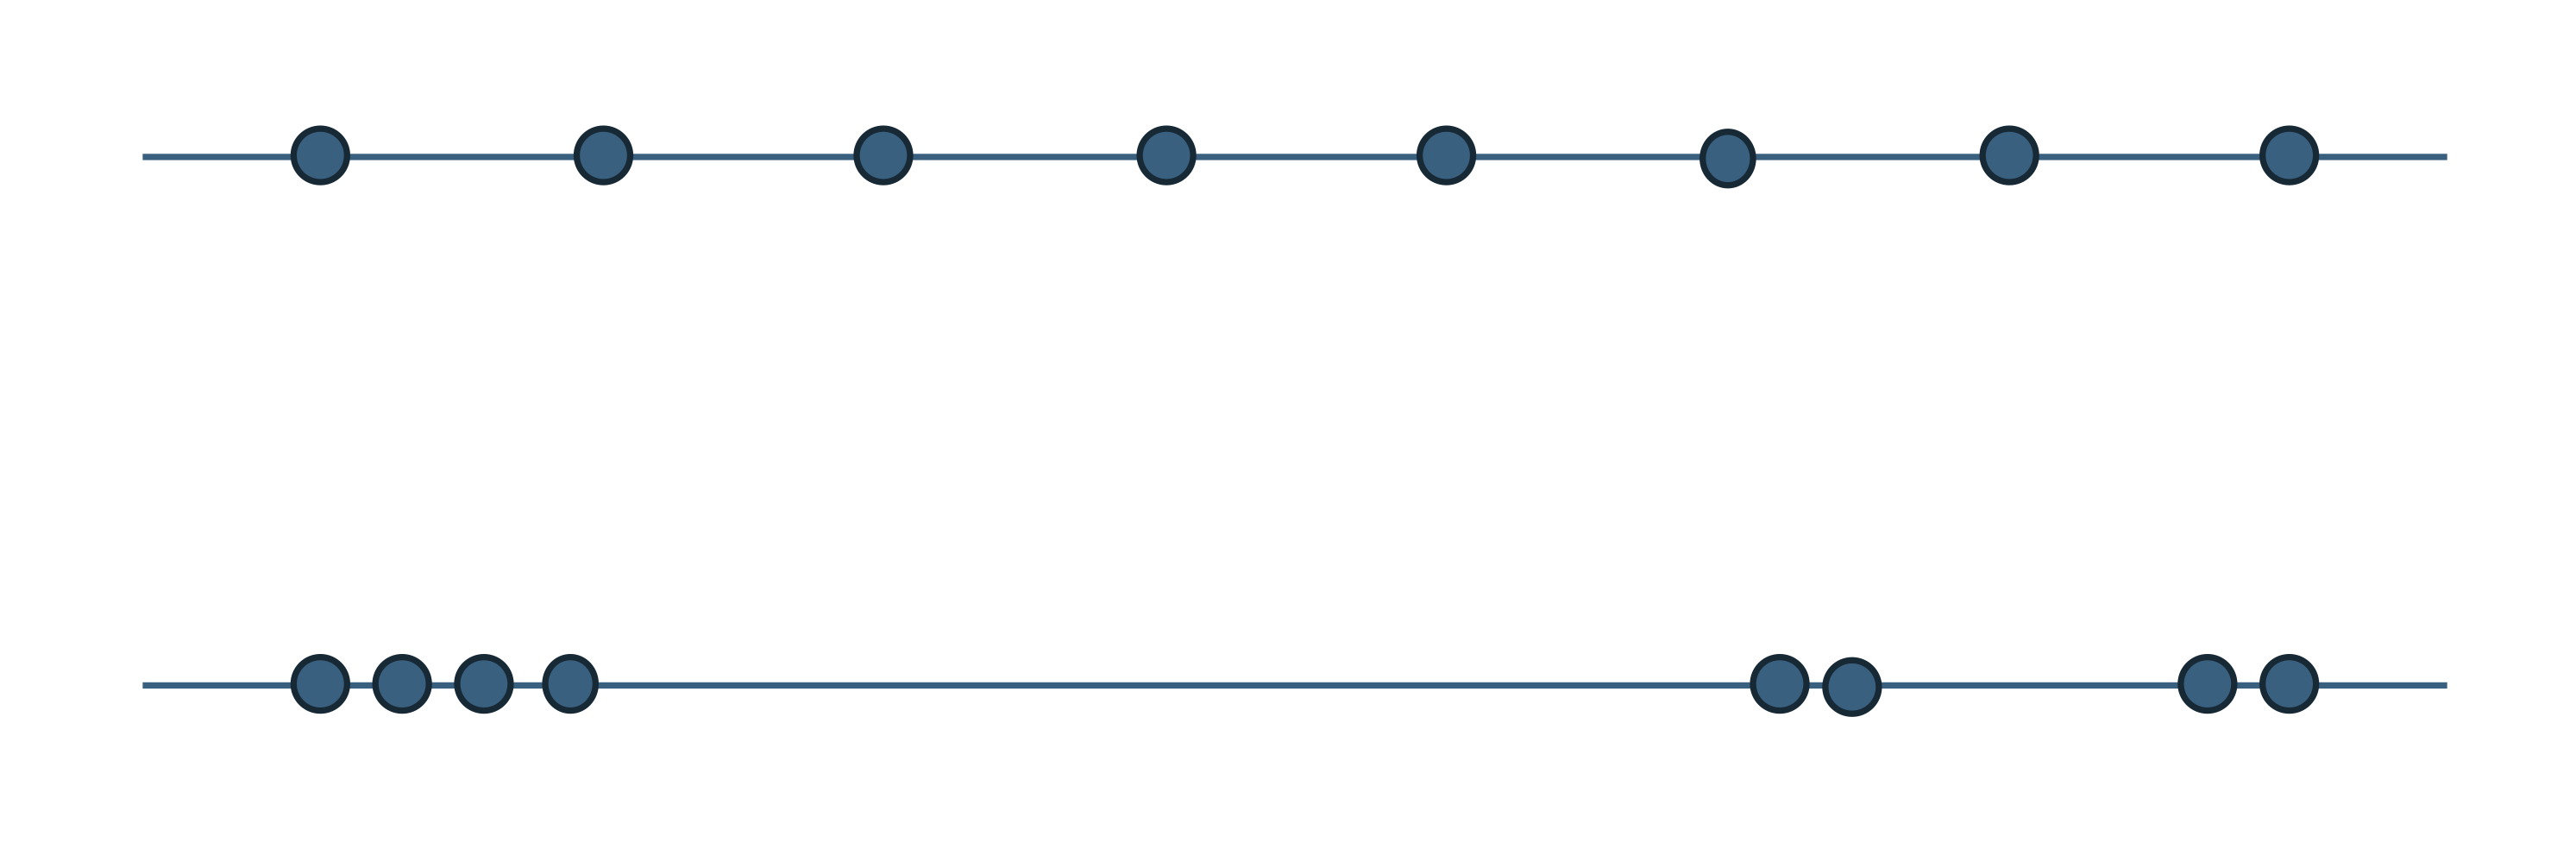
\includegraphics[width=0.7\linewidth]{\toplevelprefix/chapters/chapter3/figs/one-dim-distribution.png}
	\caption{Eight points observed on a line.}
	\label{fig:1d-line}
\end{figure}
\end{example}


% If the (geometric) volume is not a suitable measure of parsimony or compression for a (finite-sampled empirical) distribution, then maybe the {entropy}, or {\em the minimum coding rate}, associated with true probability (density or distribution) of those samples $p(\vx_i)$ is a better measure. Although many results like Theorem \ref{thm:distribution-convergence} \yima{missing reference...} ensure convergence to the true distribution (hence entropy) in the asymptotic regime\footnote{That is, when the sample size goes to infinity.}, it is not so clear when and how one can simultaneously infer the distribution and conduct the compression correctly in the {\em non-asymptotic} regime when we are given only a fixed set of samples, as the cases shown in Figure \ref{fig:1d-line}. It is observed empirically that sampling Algorithm \ref{alg:iterative_denoising} (with diffusion/denoising models) tends to generalize beyond just generating samples from the training set.

% Furthermore, besides the entropy of the data distribution, there are in fact other fundamental constraints and costs associated with implementing an encoding-decoding scheme for any given data set. This section attempts to address some of these issues from a constructive perspective regarding learning and representing a data distribution from a finite set of samples.


%\yima{From computable (entropy) to implementable. That is, in addition to a computable or achievable encoding scheme, there should also exist an implementable decoding scheme. Lossy quantization becomes necessary for real-valued data.}

There is yet another technical difficulty associated with constructing an explicit encoding and decoding scheme for a data set. Given a sampled data set in $\X = [\vx_1, \ldots, \vx_N]$, how to design a coding scheme that is implementable on machines with finite memory and computing resources? Note that even representing a general real number requires an infinite number of digits or bits. Therefore, one may wonder whether the entropy of a distribution is a direct measure for the complexity of its (optimal) coding scheme. We examine this matter with another simple example.
\begin{example}[Precision] \label{eg:two-inrational}
	Consider a discrete distribution $\X = [e, \pi]$ with equal probability $1/2$ taking the values of the Euler number $e \approx 2.71828$ or the number $\pi \approx 3.14159$. The entropy of this distribution is $H =1$, which suggests that one may encode the two numbers by a one-bit digit $0$ or $1$, respectively. But can you realize a decoding scheme for this code on a finite-state machine? The answer is actually no, as it takes infinitely many bits to describe either number precisely.
\end{example}

Hence, it is generally impossible to have an encoding and decoding scheme that can precisely reproduce samples from an arbitrary real-valued distribution.\footnote{That is, if one wants to encode such samples precisely, the only way is to memorize every single sample. } But there would be little practical value to encode a distribution without being able to decode for samples drawn from the same distribution.

So to ensure that any encoding/decoding scheme is computable and implementable
with finite memory and computational resources, we need to quantify the sample $\x$ and encode it only up to a certain precision, say $\epsilon > 0$. {\em By doing so, in essence, we treat any two data points equivalent if their distance is less than $\epsilon$.} More precisely, we would like to consider coding schemes
\begin{equation}
	\x \mapsto \hat \x
\end{equation}
such that the expected error caused by the quantization is bounded by $\epsilon$. It is mathematically more convenient, and conceptually almost identical, to bound the expected \textit{squared} error by \(\epsilon^{2}\), i.e., 
\begin{equation}
	\Ex[d(\vx, \hat \vx)^{2}] \le \epsilon^{2}.
\end{equation}
Typically, the distance \(d\) is chosen to be the Euclidean distance, or the
2-norm.\footnote{More generally, we can replace \(d^{2}\) with any so-called
\textit{divergence}.} We will adopt this choice in the sequel.

\subsection{Rate Distortion and Data Geometry}
Of course, among all encoding schemes that satisfy the above constraint, we
would like to choose the one that minimizes the resulting coding rate. For
a given random variable $\x$ and a precision $\epsilon$, this rate is known as
the {\em rate distortion}, denoted as $\cR_{\epsilon}(\x)$. 
A deep theorem in information theory, originally proved by
\textcite{shannon1959coding}, establishes that this rate can be expressed
equivalently in purely probabilistic terms as
\begin{equation}
	% \cR_{\epsilon}(\x) = \min_{p(\hat \x \mid \x): \Ex[\norm{\x -\hat \x}_2^{2}] \le \epsilon^{2}} [h(\x) - h(\x \mid \hat{\x})],
	\cR_{\epsilon}(\x) 
	= \min_{p(\hat \x \mid \x): \Ex[\norm{\x -\hat \x}_2^{2}] \le \epsilon^{2}} 
	I(\vx; \hat{\vx}),
    \label{eqn:rate-distortion-general}
\end{equation}
where the quantity $I(\vx; \hat{\vx})$ is known as the \textit{mutual
information}, defined by
\begin{equation}\label{eq:mutual-information}
	I(\vx; \hat{\vx})
	= \KL(p(\vx, \hat{\vx}) \mmid p(\vx) p(\hat{\vx})).
\end{equation}
Note that the minimization
in \eqref{eqn:rate-distortion-general} is over all conditional distributions $p(\hat \x \mid \x)$
that satisfy the distortion constraint $\Ex_{\x, \hat \x}[\norm{\x- \hat \x}_2^{2}] \le \epsilon^{2}$. 
Each such conditional distribution induces a joint distribution $p(\vx,
\hat{\vx}) = p(\hat\x \mid \x) p(\x)$, which determines the mutual
information \eqref{eq:mutual-information}.
Many convenient properties of the mutual information (and hence the rate
distortion) are implied by corresponding properties of the KL divergence (recall
\Cref{thm:information-inequality}).
From the definition, we know that $\cR_{\epsilon}(\x)$ is a {\em non-increasing}
function in $\epsilon$.

\begin{remark}
	As it turns out, the rate distortion is an implementable
	approximation to the entropy of $\x$ in the following sense.
	Assume that $\vx$ and $\hat{\vx}$ are continuous random vectors.
	Then the mutual information can be written as
	\begin{equation}\label{eq:information-entropy}
		I(\x; \hat\x) = h(\x) - h(\x \mid \hat \x),
	\end{equation}
	where $h(\x \mid \hat \x) = \bE[\log_2 p(\x \mid \hat\x)]$ is the
	\textit{conditional entropy} of $\x$ given $\hat \x$.
	% Notice that in Information Theory, the quantity $h(\x) - h(\x \mid \hat \x)$
	% is known as {\em the mutual information} $I(\x; \hat \x)$ between the two
	% variables $\x$ and $\hat \x$. See \cite{Cover-Thomas} for more details.
	Hence, the minimal coding rate is achieved when the difference between the
	entropy of $\x$ and the conditional entropy of $\x$ given $\hat \x$
	% between $\x$ and $\hat \x$ 
	is minimized among all distributions that satisfy
	the constraint: $\mathbb{E} [\norm{\x- \hat \x}_2^2] \le \epsilon^2$. 
	% From
	% the properties of mutual information $I(\x; \hat \x) = I(\hat \x; \x)$, we
	% have\footnote{The subsequent assertion assumes for simplicity that the reconstruction
	% $\hat{\vx}$ is also a continuous random vector, so that the differential
	% entropy is well-defined. More generally, advanced
	% mathematical notions from measure theory can be used to define the mutual
	% information irrespective of whether or not $\vx$ and $\hat{\vx}$ are
	% continuous or discrete: see \textcite[\S 8.5]{Cover-Thomas}.}
	% \begin{equation}
 %        h(\x) - h(\x \mid \hat{\x}) = h(\hat\x) - h(\hat\x \mid {\x}).
 %    \end{equation}
 %    Hence, the above rate distortion \eqref{eqn:rate-distortion-general} can also be rewritten as:
 %    \begin{equation}
	% 	\cR_{\epsilon}(\x) = \min_{p(\hat \vx \mid \vx): \mathbb{E} [\norm{\x-
	% 	\hat \x}_2^{2}] \le \epsilon^{2}} [H(\hat \x) - H(\hat \x \mid \x)].  \label{eqn:rate-distortion-general-2}
	% \end{equation}

	In fact, it is not necessary to assume that $\x$ and $\hat \x$ are continuous
	to obtain the above type of conclusion. For example, if both random vectors
	are instead discrete, we have after a suitable interpretation of the KL
	divergence for discrete-valued random vectors that
	\begin{equation}
		I(\x; \hat\x) = H(\x) - H(\x \mid \hat \x).
	\end{equation}
	More generally, advanced mathematical notions from measure theory can be
	used to define the mutual information (and hence the rate distortion) for
	arbitrary random variables $\x$ and $\hat \x$, including those with rather
	exotic low-dimensional distributions; see \textcite[\S 8.5]{Cover-Thomas}.
\end{remark}

\begin{remark}
    Given a set of data points in $\X = [\x_1,\ldots, \x_N]$, one can always
	interpret them as samples from a uniform discrete distribution with equal
	probability $1/N$ on these $N$ vectors. The entropy for such a distribution
	is $H(\X) = \frac{1}{N}\log_2 N$.\footnote{Note again, even if we can encode
	these vectors with this coding rate, we cannot decode them with an arbitrary
	precision.} However, even if $\X$ is  a uniform distribution on its samples,
	the coding rate $\cR_{\epsilon}(\X)$ achievable with a lossy coding scheme
	could be significantly lower than $H(\X)$ if these samples are not so evenly
	distributed and many are clustered closely to each other. Therefore, for the
	second distribution shown in Figure \ref{fig:1d-line}, for a properly chosen
	quantization error  $\epsilon$, the achievable lossy coding rate can be
	significantly lower than coding it as a uniform
	distribution.\footnote{Nevertheless, for this discrete uniform distribution,
	when $\epsilon$ is small enough, we always have $H(\X) \approx \cR_{\epsilon}(\X)$.} Also notice that, with the notion of rate distortion, the difficulty discussed in Example \ref{eg:two-inrational} also disappears: We can choose two rational numbers that are close enough to each of the two irrational numbers. The resulting coding scheme will have a finite complexity. 
\end{remark}

\begin{example}\label{example:sphere-covering-rate-distortion}
	Sometimes, one may face an opposite situation when we want to fix the coding
	rate first and try to find a coding scheme that minimizes the distortion.
	For example, suppose that we only want to use a fixed number of codes for
	points sampled from a distribution, and we want to know how to design the
	codes such that the average or maximum distortion is minimized during the
	encoding/decoding scheme. For example, given a uniform distribution on
	a unit square, we wonder how precisely we can encode points drawn from this
	distribution, with say $n$ bits. This problem is equivalent to asking what
	is the minimum radius (i.e., distortion) such that we can cover the unit
	square with $2^n$ discs of this radius. Figure
	\ref{fig:seven-circles-packing} shows approximately optimal coverings of
	a square with \(n = 4, 6, 8\), so that \(2^{n} = 16, 64, 256\) discs, respectively. Notice that the optimal radii of the discs decreases as the number of discs \(2^{n}\) increases.
	\begin{figure}
		\centering
		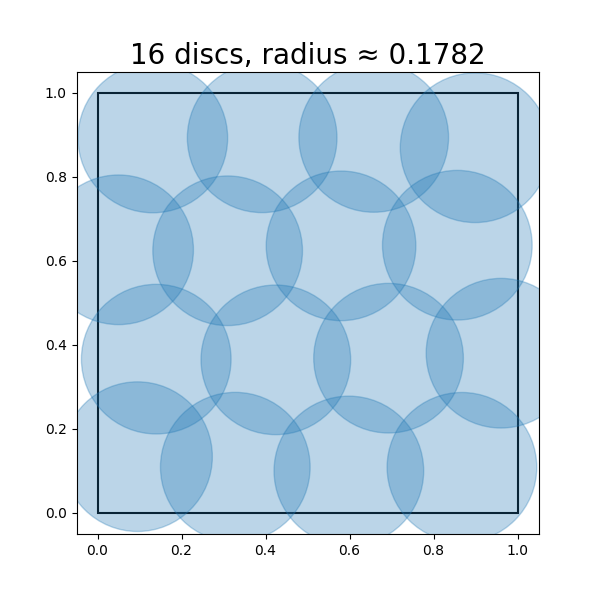
\includegraphics[width=0.3\textwidth]{\toplevelprefix/chapters/chapter3/figs/16.png}
		\hfill
		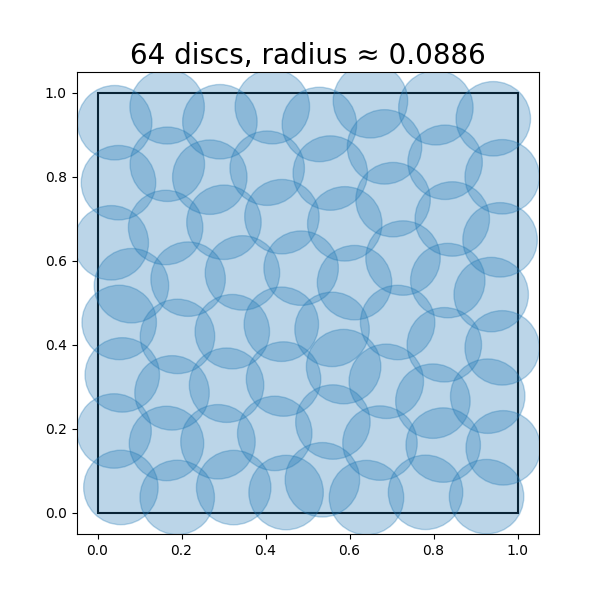
\includegraphics[width=0.3\textwidth]{\toplevelprefix/chapters/chapter3/figs/64.png}
		\hfill
		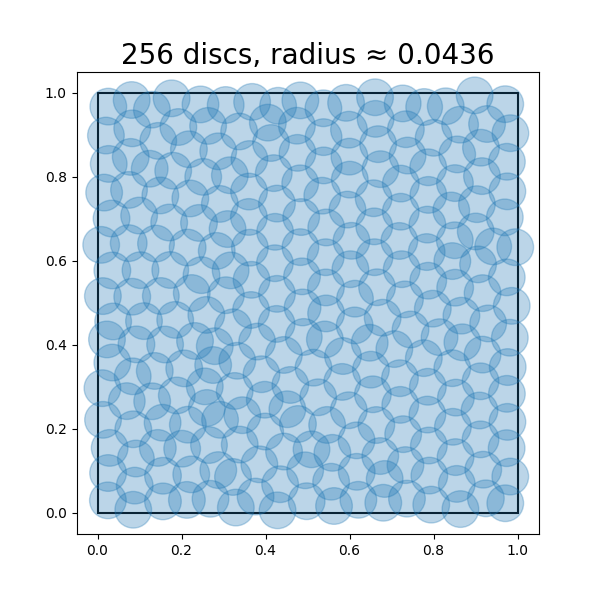
\includegraphics[width=0.3\textwidth]{\toplevelprefix/chapters/chapter3/figs/256.png}

		\caption{Approximations to the optimal solutions for \(2^{4}\),
		\(2^{6}\), and \(2^{8}\) discs covering a square, along with the
		corresponding radii, calculated using a heuristic optimization algorithm.}
		\label{fig:seven-circles-packing}
	\end{figure}
\end{example}

\begin{figure}[t]
	\centering 
	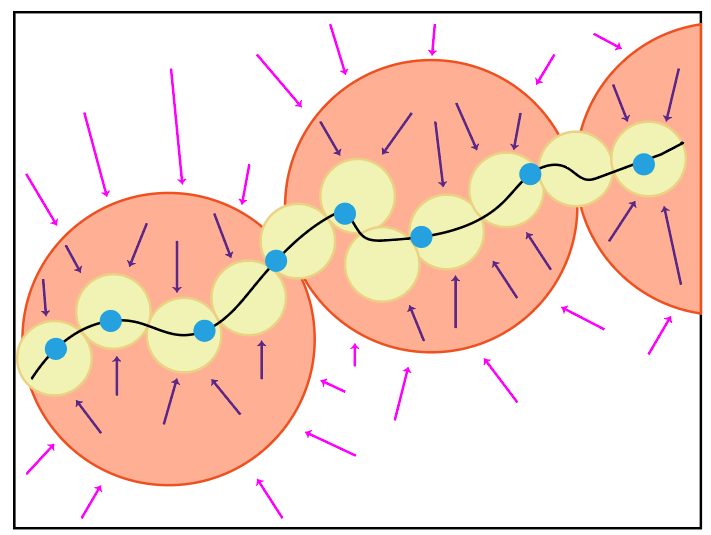
\includegraphics[width=0.6\textwidth]{\toplevelprefix/chapters/chapter3/figs/continuation.png}
	\caption{\small\textbf{The approximation of a low-dimensional distribution
	by \(\epsilon\) balls.} We can see that as the \(\epsilon\) parameter
	shrinks, the union of \(\epsilon\)-balls approximates the support of the
	true distribution (black) increasingly well. Furthermore, the associated
	denoisers (whose input-output mapping is given by the provided arrows)
	obtained by approximating the true distribution by a mixture of Gaussians,
	each with covariance \((\epsilon^{2}/D)\vI\), increasingly well-approximate
	the true denoisers. At large \(\epsilon\), such denoisers do not point near
	the true distribution at all, whereas at small \(\epsilon\) they closely
	approximate the true denoisers. \Cref{thm:covering-number-rate-distortion}
	establishes that this approximation characterizes the rate distortion
	function at small distortions $\epsilon$, unifying the parallel approaches
	of coding rate minimization and denoising for learning low-dimensional
	distributions without pathologies.}
	\label{fig:continuation}
\end{figure}

It turns out to be a notoriously hard problem to obtain closed-form expressions
for the rate distortion function \eqref{eqn:rate-distortion-general} for general
distributions $p(\vx)$. However, as
\Cref{example:sphere-covering-rate-distortion} suggests, there are important
special cases where the \textit{geometry} of the support of the distribution
$p(\vx)$ can be linked to the rate distortion function, and hence to the optimal
coding rate at distortion level $\epsilon$.
In fact, this example can be generalized to any setting where the
support of $p(\x)$ is a sufficiently regular compact set---including
low-dimensional distributions---and $p(\x)$ is uniformly distributed on its
support.
This covers a vast number of cases of practical interest.
We formalize this notion in the following result, which establishes this
property for a special case.


% \DP{BEGIN SUS STUFF}
%
% The above example can be generalized to show that the rate distortion of a random variable \(\vx\) is very closely related to the so-called \textit{covering number} of the support of \(\vx\), given that this support is a compact set (e.g., bounded). Indeed, the covering number is exactly the number of balls with a finite radius that can cover the support of \(\vx\). We formalize this notion in the following proposition, to be proved in \Cref{exer:prop cover}.

\begin{theorem}\label{thm:covering-number-rate-distortion}
	Suppose that \(\vx\) is a random variable such that its support \(K \doteq \Supp(\vx)\) is a compact set. Define the \textit{covering number} \(\cN_{\epsilon}(K)\) as the minimum number of balls of radius \(\epsilon\) that can cover \(K\), i.e.,
	\begin{equation}
		\cN_{\epsilon}(K) \doteq \min\left\{n \in \bN \colon \exists \vp_{1}, \dots, \vp_{n} \in K\ \text{s.t.}\ K \subseteq \bigcup_{i = 1}^{n}B_{\epsilon}(\vp_{i})\right\},
	\end{equation}
	where \(B_{\epsilon}(\vp) = \set{\vxi\in \R^D \given \norm{\vxi - \vp}_2 \leq
	\epsilon}\) is the Euclidean ball of radius \(\epsilon\) centered at \(\vp\).
	Then it holds 
	\begin{equation}
		\cR_{\epsilon}(\vx) 
		\leq \log_{2} \cN_{\epsilon}(K).
	\end{equation}
	If, in addition, $\vx$ is uniformly distributed on $K$ and $K$ is
	a mixture of mutually orthogonal low-rank subspaces,\footnote{In fact, it is
	possible to treat highly irregular $K$, such as fractals, with a parallel
	result, but its statement
	becomes far more technical: c.f.\ Riegler et al.\
	\cite{Riegler2018-jh,Riegler2023-rr}. We give a simple proof in
	\Cref{app:rate-distortion-covering} which shows the result for mixtures of
	subspaces.}
	then a matching lower bound holds:
	\begin{equation}
		\cR_{\epsilon}(\vx)
		\geq
		\log_{2} \cN_{\epsilon}(K) - O(D).
	\end{equation}
\end{theorem}
\begin{proof}
A proof of this theorem is beyond the scope of this book and we defer it to \Cref{app:rate-distortion-covering}.
\end{proof}

% The proof of the upper bound in \Cref{thm:covering-number-rate-distortion} is
% a straightforward exercise left to the reader, using the fact that \textit{any}
% covering of $\Supp(\vx)$ by
% $\epsilon$-balls having cardinality $N$ induces a (deterministic) coding scheme
% for $\vx$ with rate at most $N$ and expected squared distortion no larger than
% $\epsilon^2$.
%

The implication of \Cref{thm:covering-number-rate-distortion} can be summarized
as follows: for sufficiently accurate coding of the distribution of
$\x$, the minimum rate distortion coding framework is completely characterized
by the sphere packing problem on the support of $\x$. 
The core of the proof of \Cref{thm:covering-number-rate-distortion} can indeed
be generalized to more complex distributions such as sufficiently incoherent
mixtures of manifolds, but we leave this for a future study.
% If \(\vx\) does not have a compact support, but is benign (for example, having
% Gaussian-like tails), then it can be approximated by a compactly supported
% random variable,\footnote{Say by normalizing it to some large unit ball of radius \(R\),
% i.e., \(\vx \mapsto (\vx/\norm{\vx}_{2}) \cdot \min(R, \|\vx\|_{2})\).} at which
% point \Cref{thm:covering-number-rate-distortion} applies. 
So the rate distortion can be thought of as a ``probability-aware'' way to
approximate the support of the distribution of
\(\vx\) by a mixture of many small balls.
% A visualization of this whole situation is given in \Cref{fig:continuation}.

We now discuss another connection between this and the
denoising-diffusion-entropy complexity hierarchy we discussed earlier in the
Chapter.

\begin{remark}\label{rem:slb}
	The key ingredient in the proof of the lower bound in
	\Cref{thm:covering-number-rate-distortion} is an important result from
	information theory known as the \textit{Shannon lower bound} for the rate
	distortion, named after Claude Shannon, who first derived it in a special case
	\cite{shannon1959coding}. It
	asserts the following estimate for the rate distortion function, for any random
	variable $\x$ with
	a density $p(\x)$ and finite expected squared norm \cite{Linder1994-ej}:
	\begin{equation}\label{eq:slb}
		\cR_{\epsilon}(\x)
		\geq
		h(\x)
		- \log_2 \volume(B_{\epsilon})
		-
		C_D,
		% \log
		% \left(
		% \frac{
		% 	2
		% }
		% {
		% 	d \Gamma(d/2)
		% }
		% \left(
		% \frac{
		% 	de
		% }
		% {
		% 	2
		% }
		% \right)^{d/2}
		% \right)
	\end{equation}
	where $C_D > 0$ is a constant depending only on $D$. Moreover, this lower bound
	is actually sharp as $\epsilon \to 0$: that is,
	\begin{equation}
		\lim_{\epsilon \to 0} \cR_{\epsilon}(\x) - \left[ h(\x) - \log_2
		\volume(B_{\epsilon}) - C_D\right] = 0.
	\end{equation}
	So when the distortion $\epsilon$ is small, we can think solely in terms of
	the Shannon lower bound, rather than the (generally intractable)
	optimization problem defining the rate distortion
	\eqref{eqn:rate-distortion-general}.

	The Shannon lower bound is the bridge between the coding rate, entropy
	minimization/denoising, and geometric sphere packing approaches for learning
	low-dimensional distributions. Notice that in the special case of a uniform
	density $p(\x)$, \eqref{eq:slb} becomes
	\begin{align}
		\cR_{\epsilon}(\x) &\geq -\int_K \frac{1}{\volume(K)} \log_2
		\frac{1}{\volume(K)} \odif \vxi
		- \log_2 \volume(B_{\epsilon}) - C_d
		\\
		&=
		% \log_2 \volume(K)
		% - \log \volume(B_{\epsilon}) - C_d.
		\log_2 \volume(K) / \volume(B_{\epsilon})
		- C_d. \label{eq:shannon-lower-bound-uniform}
	\end{align}
	The ratio $\volume(K) / \volume(B_{\epsilon})$ approximates the number of
	$\epsilon$-balls needed to cover $K$ by a worst-case argument, which is
	accurate for sufficiently regular sets $K$ when $\epsilon$ is small (see
	\Cref{app:rate-distortion-covering} for details).
	Meanwhile, recall the Gaussian denoising model $\x_{\epsilon} = \x
	+ \epsilon \vg$ from
	earlier in the Chapter, where $\vg \sim \cN(\Zero, \vI)$ is independent of
	$\x$.
	Interestingly, the differential entropy of the joint distribution $(\vx,
	\vg)$
	can be calculated as
	% Then the differential
	% entropy of $x_{\epsilon}$ is approximately given by
	\begin{align}
		h(\vx, \vg)
		% &\approx
		&=
		-\int
		p(\vxi) p(\vgamma) \log_2 p(\vxi) p(\vgamma) \odif \vxi \odif \vgamma
		\\
		&=
		h(\x) + h(\epsilon \vg).
	\end{align}
	We have seen the Gaussian entropy calculated in
	\Cref{eqn:entropy-Gaussian-multi}: when $\epsilon$ is small, it is equal, up
	to additive constants, to the volumetric quantity $-\log_2
	\volume(B_{\epsilon})$ we have seen in the Shannon lower bound.
	In certain special cases (e.g., data supported on incoherent low-rank subspaces),
	when $\epsilon$ is small and the support of $\x$ is sufficiently regular,
	the distribution of $\x_{\epsilon}$ can even be well-approximated locally by the
	product of the distributions $p(\x)$ and $p(\vg)$, justifying the above
	computation. 
	Hence the Gaussian denoising process yields yet another interpretation of
	the Shannon lower bound, as arising from the entropy of a noisy version of
	$\x$, with noise level proportional to the distortion level $\epsilon$.


	Thus, this finite rate distortion approach via sphere covering re-enables or
	generalizes all previous measures of complexity of the distribution, allowing us
	to differentiate between and rank different distributions in a unified way.
	These interrelated viewpoints are visualized in \Cref{fig:continuation}.
\end{remark}




% \sdb{Begin Sus}
%
% % The inequality is tight in some simple cases (such as $\vx$ being distributed on the interval $[0, \alpha\epsilon]$ where $\alpha$ is an integer).
% If \(\vx\) does not have a compact support, but is benign (for example, having Gaussian-like tails), then it can be approximated by a compactly supported random variable (say by normalizing it to some large unit ball of radius \(R\), i.e., \(\vx \mapsto (\vx/\norm{\vx}_{2}) \cdot \min(R, \|\vx\|_{2})\)), at which point the above theorem applies. So the rate distortion can be thought of as a ``probability-aware'' way to approximate the support of the distribution of \(\vx\) by a mixture of many small balls.
%
%
%
% \begin{remark}
% 	For small but finite \(\epsilon\), working with the distribution of the lossy encoding \(\hat \vx\) instead of the raw data \(\vx\) is much easier. While it approximates the distribution of \(\vx\), it is discrete, hence having a well-defined entropy; it also has a well-defined volume. Thus, this finite rate distortion approach via sphere covering re-enables or generalizes all previous measures of complexity of the distribution, allowing us to differentiate between and rank different distributions in a unified way.
%
% 	In particular, supposing for simplicity that \(\vx\) is uniformly distributed on a compact set (which may be low-dimensional), one has the following remarkable identities relating the properties of \(\hat{\vx}\) to the properties of \(\vx\). Recalling that \(\hat{\vx}\) depends on \(\epsilon\), and letting \(V_{D}(\epsilon) = C_{D}\epsilon^{D}\) be the volume of an \(\epsilon\)-ball in \(\R^{D}\) (where \(C_{D}\) is a constant that depends on the dimension \(D\)), we have that
% 	\begin{align}
% 		\operatorname{vol}(\Supp(\vx))
% 		&\geq  \lim_{\epsilon \to 0}V_{D}(\epsilon)2^{\cR_{\epsilon}(\vx)}, \\
% 		\dim(\Supp(\vx))
% 		&\geq \lim_{\epsilon \to 0}\frac{\cR_{\epsilon}(\vx)}{\log(1/\epsilon)}, \\
% 		h(\vx)
% 		&= \lim_{\epsilon \to 0}\bs{\cR_{\epsilon}(\vx) + H(\hat{\vx} \mid \vx) + \log V_{D}(\epsilon)}.
% 	\end{align}
% 	The first and second expression follow from the interpretation of the coding rate or rate distortion as a lower bound on the covering. The second in particular follows from the definition of the Minkowski dimension \citep{bishop2017fractals} and holds whenever the support of \(\vx\) is not too pathological (e.g., a low-dimensional manifold). The third follows from expanding the integral definition of differential entropy for \(\vx\) and approximating it with an appropriate Riemann sum, then writing for the resulting entropy \(H(\hat{\vx}) = \cR_{\epsilon}(\vx) + H(\hat{\vx} \mid \vx)\); filling in the details of this proof is left as an exercise. A visualization of this whole situation is given in \Cref{fig:continuation}.
%
% 	While some of the arguments to the three limits diverge to \(\infty\) as \(\epsilon \to 0\), they can still be compared at finite \(\epsilon\) as good approximations. Thus we can understand all previous measures of complexity strictly in terms of the rate distortion at finite \(\epsilon\).
% \end{remark}
%
% \DP{END SUS STUFF}

For a general distribution at finite distortion levels, it is typically impossible to find its rate
distortion function in an analytical form. One must often resort to numerical computation\footnote{Interested readers may refer to \cite{Blahut-1972} for a classic algorithm that computes rate distortion function numerically for a discrete distribution.}.  Nevertheless, as we will see, in our context, we often need to know the rate distortion as an explicit function of a set of data points or their representations. This is because we want to use the coding rate as a measure of the goodness of the representations. An explicit analytical form makes it easy to determine how to transform the data distribution to improve the representation. So, we should work with distributions whose rate distortion functions take explicit analytical forms. To this end, we start with the simplest, and also the most important, family of distributions.

\subsection{Lossy Coding Rate for a Low-Dimensional Gaussian}\label{subsec:lossy DR}
%\yima{Lossy coding length, encoding and decoding via sphere packing, rate distortion for a Gaussian or a low-dimensional subspace. }
Now suppose we are given a set of data samples in $\X = [\x_1, \ldots, \x_N]$ from any distribution.\footnote{Or these data points could be viewed as an (empirical) distribution themselves.} We would like to come up with a constructive scheme that can encode the data up to certain precision, say
\begin{equation}
	\x_i \mapsto \hat \x_i, \quad \mbox{subject to} \quad \|\x_i - \hat \x_i\|_2 \le \epsilon.
\end{equation}
Notice that this is a sufficient, explicit, and interpretable condition which
ensures that the data are encoded such that \(\frac{1}{N}\sum_{i = 1}^{N}
\norm{\x_i- \hat \x_i}_2^{2} \le \epsilon^{2}\). This latter inequality is exactly the rate distortion constraint for the provided empirical distribution and its encoding. For example, in \Cref{example:sphere-covering-rate-distortion}, we used this simplified criterion to explicitly find the minimum distortion and explicit coding scheme for a given coding rate.

Without loss of generality, let us assume the mean of $\X$ is zero, i.e., $\frac{1}{N} \sum_{i = 1}^{N} \x_i = \boldsymbol{0}$. Without any prior knowledge about the nature of the distribution behind $\X$, we may view $\X$ as sampled from a Gaussian distribution $\mathcal{N}(\boldsymbol{0}, {\boldsymbol{\Sigma}})$ with the covariance\footnote{It is known that given a fixed variance, the Gaussian achieves the maximal entropy. That is, it gives an upper bound for what the worst case could be in terms of possible coding rate.}
\begin{equation}
	{\boldsymbol{\Sigma}} = \frac{1}{N} \X\X^\top.
\end{equation}
Notice that geometrically ${\boldsymbol{\Sigma}}$ characterizes an ellipsoidal region where most of the samples $\x_i$ reside.

We may view $\hat \X = [\hat \x_1,\ldots, \hat \x_N]$ as a noisy version of $\X = [\x_1, \ldots, \x_N]$:
\begin{equation}
	\hat \x_i = \x_i + \vw_i,
\end{equation}
where $\vw_i$ is a Gaussian noise $\vw_i  \sim \mathcal{N}(\boldsymbol{0} , {\epsilon^2}  \boldsymbol{I}/{D})$ independent of $\vx_i$. Then the covariance of $\hat \x_i$ is given by
\begin{equation}
	\hat{\boldsymbol{\Sigma}} = \mathbb{E}\left[\hat \x_i \hat \x_i^\top\right] = \frac{\epsilon^2}{D} \boldsymbol{I} + \frac{1}{N} \X\X^\top.
\end{equation}
Note that the volume of the region spanned by the vectors $\x_i$ is proportional to the square root of the determinant of the
covariance matrix
\begin{equation}
	\mbox{volume}(\hat \x_i) \propto \sqrt{\det \big(\hat{\boldsymbol{\Sigma}}\big)} = \sqrt{\det\left(\frac{\epsilon^2}{D} \boldsymbol{I} + \frac{1}{N} \X\X^\top \right)}.
\end{equation}
The volume spanned by each random vector $\boldsymbol{w}_i$ is
proportional to
\begin{equation}
	\mbox{volume}(\boldsymbol{w}_i) \propto   \sqrt{\det\left(\frac{\epsilon^2}{D} \boldsymbol{I} \right)}.
\end{equation}

\begin{figure}
	\centering
	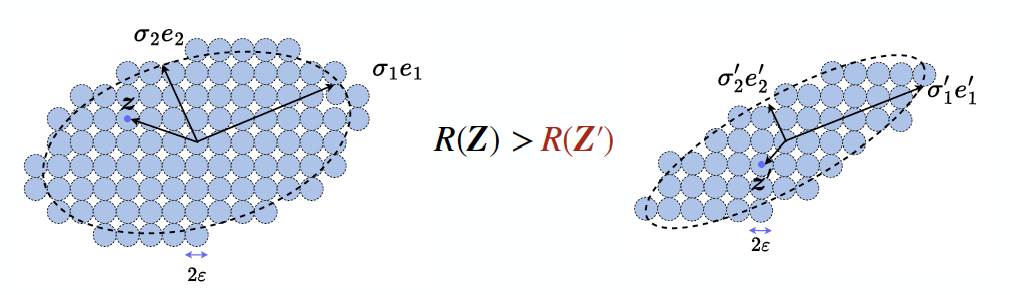
\includegraphics[width=\linewidth]{\toplevelprefix/chapters/chapter3/figs/Gaussian-compression.png}
	\caption{Covering the region spanned by the data vectors using $\epsilon$-balls. The larger the volume of the space, the more balls are needed, hence the more bits are needed to encode and enumerate the balls. Each real-valued vector $\vx$ can be encoded as the number of the ball which it falls into.}
	\label{fig:ball-packing}
\end{figure}

To encode vectors that fall into the region spanned by $\hat \x_i$, we can cover the region with non-overlapping
balls of radius $\epsilon$, as illustrated in Figure \ref{fig:ball-packing}. When the volume of the region spanned by $\hat \x_i$ is significantly larger than the volume of the $\epsilon$-ball, the total number of balls that we need to cover the region is
approximately equal to the ratio of the two volumes:
\begin{equation}
	\# \,\epsilon\mbox{-balls} \approx \frac{\mbox{volume}(\hat \vx_i)}{\mbox{volume}(\vw_i)} = \sqrt{\det\left(\boldsymbol{I} + \frac{D}{N\epsilon^2} \X\X^\top  \right)}.
\end{equation}
If we use binary numbers to label all the $\epsilon$-balls in the region of
interest, the total number of binary bits needed is thus %\DP{suggest using notation \(R_{\eps}\) since the ``conditional'' notation will become overused in future.}
\begin{equation} 
	\cR_{\epsilon}(\X) \approx %\doteq 
	\log_2 (\# \,\epsilon\mbox{-balls}) \approx R_{\epsilon}(\X) \doteq \frac{1}{2} \log \det \left(\boldsymbol{I} + \frac{D}{N\epsilon^2} \X\X^\top \right).
	\label{eqn:rate-Gaussian}
\end{equation}

\begin{example}
	Figure \ref{fig:ball-packing} shows an example of a 2D distribution with an ellipsoidal support -- approximating the support of a 2D Gaussian distribution. The region is covered by small balls of size $\epsilon$. All the balls are numbered from $1$ to say $n$. Then given any vector $\x$ in this region, we
	only need to determine to which $\epsilon$-ball center it is the closest, denoted as $\operatorname{ball}_{\epsilon}(\x)$. To remember $\x$, we only need to remember the number of this ball, which takes $\log(n)$ bits to store. If we need to decode $\x$ from this number, we simply take $\hat \x$ as the center of the ball. This leads to an explicit encoding and decoding scheme:
	\begin{equation}
		\x \longrightarrow \operatorname{ball}_{\epsilon}(\x) \longrightarrow \hat \x = \mbox{center of} \operatorname{ball}_{\epsilon}(\x).
	\end{equation}
	One may refer to these ball centers as  ``codes'' of a code book or a dictionary for the encoding scheme. It is easy to see that the accuracy of this (lossy) encoding-decoding scheme is about the radius of the ball $\epsilon$. 
	Clearly $\cR_{\epsilon}(\Z)$ is the average
	number of bits required to encode the ball number of each vector $\z$ with
	this coding scheme, and hence can be called the {\em coding rate} associated with this scheme.
\end{example}


From the above derivation, we know that the coding rate $\cR_{\epsilon}(\X)$ is (approximately) achievable with an explicit encoding (and decoding) scheme. It has two interesting  properties:
\begin{itemize}
	\item First, one may notice that $R_{\epsilon}(\X)$ closely resembles the rate distortion function of a Gaussian source \cite{Cover-Thomas}. Indeed, when $\epsilon$ is small, the above expression is a close approximation to the rate distortion of a Gaussian source, as pointed out by   \cite{MaY2007-PAMI}.
	\item Second, the same closed-form coding rate $R_{\epsilon}(\X)$ can be derived as an approximation of \(\cR_{\epsilon}(\vX)\) if the data $\X$ are assumed to be from a linear subspace. This can be shown by properly quantifying the singular value decomposition (SVD) of $\X = \boldsymbol{U} \boldsymbol{\Sigma}\boldsymbol{V}^\top$ and constructing a lossy coding scheme for vectors in the subspace spanned by $\boldsymbol{U}$ \cite{MaY2007-PAMI}.
\end{itemize}
In our context, the closed-form expression $R_{\epsilon}(\X)$ is rather fundamental: it is the coding rate associated with an explicit and natural lossy coding scheme for data drawn from either a Gaussian distribution or a linear subspace. As we will see in the next chapter, this formula plays an important role in understanding the architecture of deep neural networks.


\subsection{Clustering a Mixture of Low-Dimensional Gaussians}
\label{sec:clustering-Gaussians}
As we have discussed before, the given dataset $\X$ often has low-dimensional intrinsic structures. Hence, encoding it as a general Gaussian would be very redundant. If we can identify those intrinsic structures in $\X$, we could design much better coding schemes that give much lower coding rates. Or equivalently, the codes used to encode such $\X$ can be compressed. We will see that compression gives a unifying computable way to identify such structures. In this section, we demonstrate this important idea with the most basic family of low-dimensional structures: a mixture of (low-dimensional) Gaussians or subspaces.

\begin{example}
	Figure \ref{fig:two-subspaces} shows an example in which the data $\X$ are distributed around two subspaces (or low-dimensional Gaussians). If they are viewed and coded together as one single Gaussian, the associated discrete (lossy) code book, represented by all the blue balls, is obviously very redundant. We can try to identify the locations of the two subspaces, denoted by $S_1$ and $S_2$, and design a code book that only covers the two subspaces, i.e., the green balls. If we can correctly partition samples in the data $\X$ into the two subspaces: $\X = [\X_1, \X_2]\bm \Pi$ with $\X_1 \in S_1$ and $\X_2 \in S_2$, where $\bm \Pi$ denotes a permutation matrix, then the resulting coding rate for the data will be much lower. This gives a more parsimonious, hence more desirable, representation of the data.
\end{example}

\begin{figure}
	\centering
	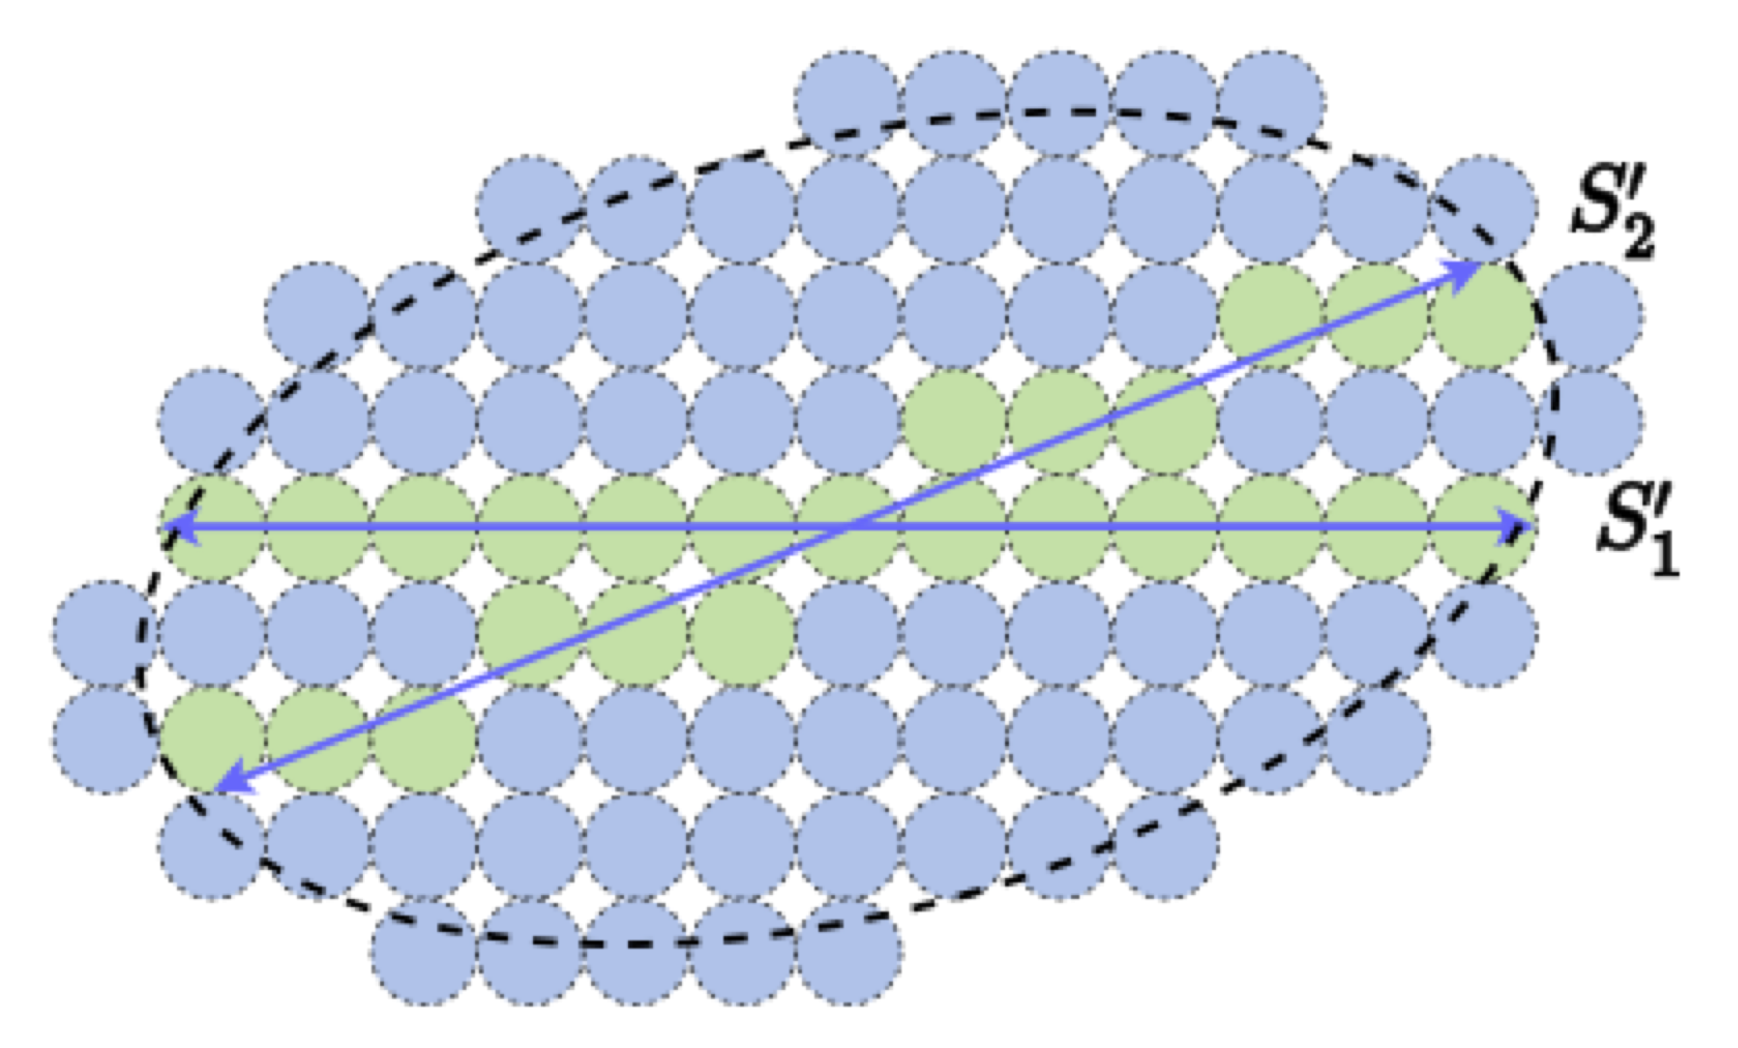
\includegraphics[width=0.5\linewidth]{\toplevelprefix/chapters/chapter3/figs/Two-subspaces.png}
	\caption{Comparison of two lossy coding schemes for data that are distributed around two subspaces. One is to pack (blue) $\epsilon$-balls for the entire space spanned by the two subspaces; the other is to pack balls only in a tabular neighborhood around the two subspaces. The latter obviously has a much smaller code book and results in a much lower coding rate for samples on the subspaces.}
	\label{fig:two-subspaces}
\end{figure}

So, more generally speaking, if the data are drawn from any mixture of subspaces or low-dimensional Gaussians, it would be desirable to identify those components and encode the data based on the intrinsic dimensions of those components. It turns out that we do not lose much generality by assuming that the data are drawn from a mixture of low-dimensional Gaussians. This is because a mixture of Gaussians can closely approximate most general distributions \cite{borkar2016gaussian}. 

\paragraph{The clustering problem.}
Now for this specific family of distributions, how can we effectively and efficiently identify those low-dimensional components from a set of samples
\begin{equation}
	\X = \left[\x_1, \x_2, \ldots, \x_N\right],
\end{equation}
drawn from them? In other words, given the whole data set $\X$, we want to partition, or cluster, it into multiple, say $K$, subsets:
\begin{equation}
	\X\bm \Pi = [\X_1, \X_2, \dots, \X_K],
\end{equation}
where each subset consists of samples drawn from only one low-dimensional Gaussian or subspace and $\bm \Pi$ is a permutation matrix to indicate membership of the partition. Note that, depending the situation, the partition could be either deterministic or probabilistic. As shown in \cite{ma2007segmentation}, for mixture of Gaussians, probabilistic partition does not lead to a lower coding rate. So for simplicity, we here consider a deterministic partition only.

\paragraph{Clustering via lossy compression.}
The main difficulty in solving the above clustering problem is that we normally do not know the number of clusters $K$, nor do we know the dimension of each component. There has been a long history for the study of this clustering problem. The textbook \cite{GPCA} gives a systematic and comprehensive coverage of different approaches to this problem. To find an effective approach to this problem, we first need to understand and clarify why we want to cluster. In other words, what exactly do we gain from clustering the data, compared with not to? How do we measure the gain? From the perspective of data compression, a correct clustering should lead to a more efficient encoding (and decoding) scheme.

For any given data set $\X$, there are already two obvious encoding schemes as the baseline. They represent two extreme ways to encode the data:
\begin{itemize}
	\item Simply view all the samples together drawn as from one single Gaussian. The associated coding rate is, as derived before, given by:
	      \begin{equation}
		      \cR_{\epsilon}(\vX) \approx R_{\epsilon}(\X) = \frac{1}{2} \log \det \left(\boldsymbol{I} + \frac{D}{N\epsilon^2} \X\X^\top \right).
	      \end{equation}
	\item Simply memorize all the samples separately by assigning a different number to each sample. The coding rate would be:
	      \begin{equation}
		      \cR_0(\X) = \log(N).
	      \end{equation}
\end{itemize}


Note that either coding scheme can become the ``optimal'' solution for certain (extreme) choice of the quantization error $\epsilon$:
\begin{enumerate}
	\item {\em Lazy Regime}: If we choose $\epsilon$ to be extremely large, all samples in $\X$ can be covered by a single ball. The rate is  $\lim_{\epsilon \rightarrow \infty} \cR_\epsilon \rightarrow \frac{1}{2}\log\det (\boldsymbol{I}) = 0$.
	\item {\em Memorization Regime}: If $\epsilon$ is extremely small, every sample in $\X$  is covered by a different $\epsilon$-ball, hence the total is $N$. The rate is $\lim_{\epsilon \rightarrow 0} \cR_\epsilon \rightarrow \log(N)$.
\end{enumerate}
Note that the first scheme corresponds to the scenario when one does not care about anything interesting about the distribution at all. One does not want to spare any bit for anything informative. We call this the ``lazy regime.'' The second scheme corresponds to the scenario when one wants to decode every sample with an extremely high precision. So one would better ``memorize'' every sample. We call this the ``memorization regime.''
\begin{figure}
	\centering
	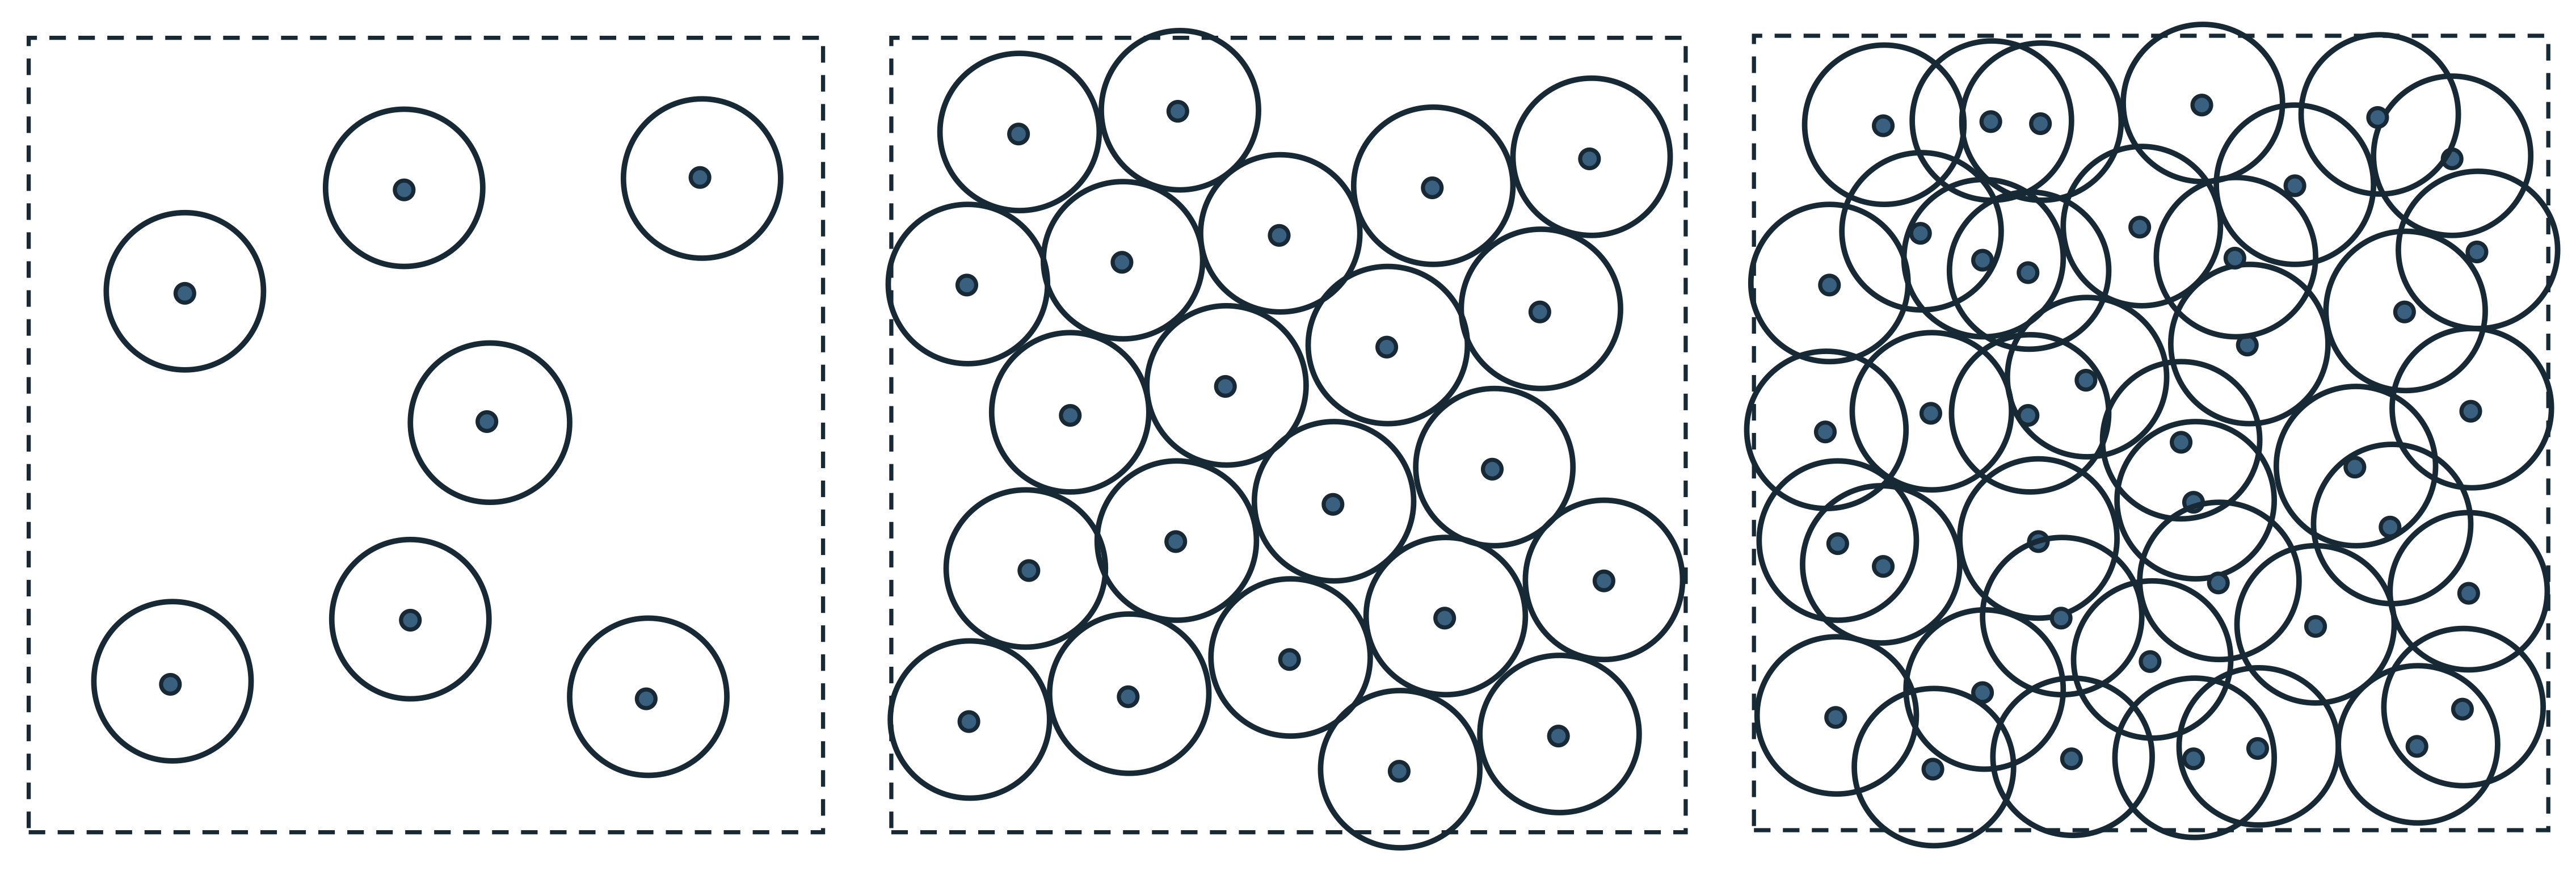
\includegraphics[width=0.9\linewidth]{\toplevelprefix/chapters/chapter3/figs/circle-packing.png}
	\caption{A number of random samples on a 2D plane. Consider an $\epsilon$-disc assigned to each sample with the sample as its center. The density of the samples increases from left to right.}
	\label{fig:circle-packing}
\end{figure}
\begin{example}
	To see when the memorization regime is preferred or not, let us consider a number, say $N$, of samples randomly distributed in a unit area on a 2D plane.\footnote{Say the points are drawn by a Poisson process with density $N$ points per unit area.} Imagine we try to design a lossy coding scheme with a fixed quantization error $\epsilon$. This is equivalent to putting an $\epsilon$-disc around each sample, as shown in Figure \ref{fig:circle-packing}. When $N$ is small, the chance that all the discs overlap with each other is zero. A codebook of size $N$ is necessary and optimal in this case. When $N$ or the density reaches a certain critical value $N_c$, with high probability all the discs start to overlap and connect into one cluster that covers the whole plane---this phenomenon is known as continuum ``percolation'' \cite{Gilbert-1961,Mertens-Moore-2012}. When $N$ becomes larger than this value, the discs overlap heavily. The number $N$ of discs becomes very redundant because we only want to encode points on the plane up to the given precision $\epsilon$. The number of discs needed to cover all the samples is much less than $N$.\footnote{In fact, there are efficient algorithms to find such a covering \cite{Booth-2001}.}
\end{example}

Both the lazy and memorization regimes are somewhat trivial and perhaps are of little theoretical or practical interest. Either scheme would be far from optimal when used to encode a large number of samples drawn from a distribution that has a {\em compact and low-dimensional support}. The interesting regime exists in between these two.
\begin{example}
	\begin{figure}[t]
		\centering
		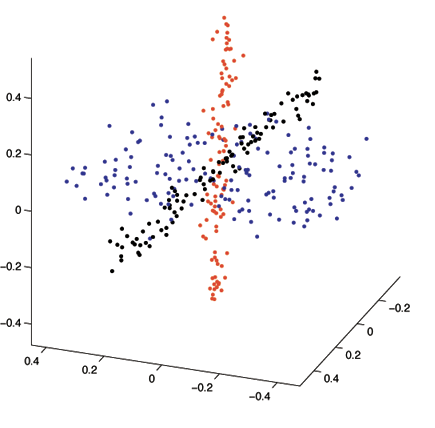
\includegraphics[width=0.4\linewidth]{\toplevelprefix/chapters/chapter3/figs/Two-lines-and-plane.png}
		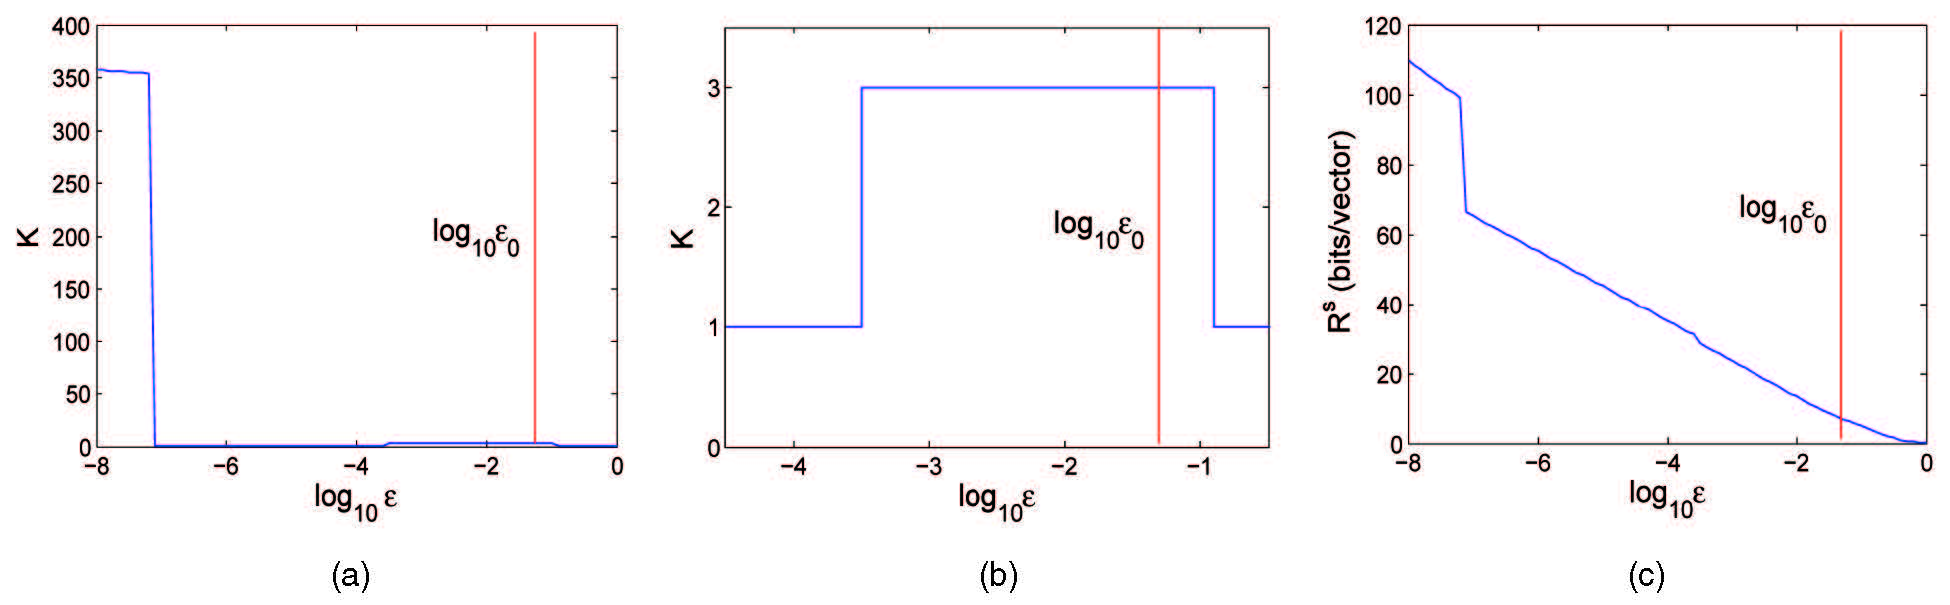
\includegraphics[width=0.9\linewidth]{\toplevelprefix/chapters/chapter3/figs/Coding-Rate.jpg}
		\caption{Top: 358  noisy samples drawn from two lines and one plane in $\mathbb{R}^3$. Bottom: the effect of varying $\epsilon$ on the clustering result and the coding rate. The red line marks the variance $\epsilon_0$ of the Gaussian noise added to the samples.}
		\label{fig:two-lines-and-plane}
		\label{fig:two-lines-and-plane-epsilon}
	\end{figure}
	Figure \ref{fig:two-lines-and-plane}  shows an example with noisy samples
	drawn from two lines and one plane in $\mathbb{R}^3$. As we notice from the
	plot (c) on the right, the optimal coding rate decreases monotonically as we
	increase $\epsilon$, as anticipated from the property of the rate distortion
	function. The plots (a) and (b) show, when varying $\epsilon$ from very
	small (near zero) to very large (towards infinite), the optimal number of
	clusters when the coding rate is minimal. We can clearly see the lazy regime
	and the memorization regime on the two ends of the plots. But one can also
	notice in plot (b), when the quantization error $\epsilon$ is chosen to be
	around the level of the true noise variance $\epsilon_0$, the optimal number
	of clusters is the ``correct'' number three that represents two planes and
	one subspace.  We informally refer to this middle regime as the
	``generalization regime''. Notice that a sharp phase transition takes place
	between these regimes.\footnote{So far, to our best knowledge, there is no rigorous theoretical justification for these phase transition behaviors.}
\end{example}


From the above discussion and examples, we see that, when the quantization error relative to the sample density\footnote{or the sample density relative to the quantization error} is in a proper range,  minimizing the lossy coding rate would allow us to uncover the underlying (low-dimensional) distribution of the sampled data. {\em Hence, quantization, started as a choice of practicality, seems to be becoming necessary for learning a continuous distribution from its empirical distribution with finite samples.} Although a rigorous theory for explaining this phenomenon remains elusive, here, for learning purposes, we care about how to exploit the phenomenon to design algorithms that can find the correct distribution.

Let us use the simple example shown in Figure \ref{fig:two-subspaces} to illustrate the basic ideas. If one can partition all samples in $\X$ into two clusters in $\X_1$ and $\X_2$, with $N_1$ and $N_2$ samples respectively, then the associated coding rate would be\footnote{We here ignore some overhead bits needed to encode the membership for each sample, say via the Huffman coding.}
\begin{equation}
	R_{\epsilon}^c(\X\mid \boldsymbol{\Pi}) = \frac{N_1}{N}R_{\epsilon}(\X_1) + \frac{N_2}{N}R_{\epsilon}(\X_2),
\end{equation}
where we use $\boldsymbol{\Pi}$ to indicate membership of the partition. If the partition respects the low-dimensional structures of the distribution, in this case $\X_1$ and $\X_2$ belonging to the two subspaces respectively, then the resulting coding rate should be significantly smaller than the above two basic schemes:
\begin{equation}
	R_{\epsilon}^c(\X \mid \boldsymbol{\Pi}) \ll R_{\epsilon}(\X), \quad     R_{\epsilon}^c(\X \mid \boldsymbol{\Pi}) \ll R_0(\X).
\end{equation}
In general, we can cast the clustering problem into an optimization problem that minimizes the coding rate:
\begin{equation}
	\min_{\boldsymbol{\Pi}}  \bc{ R_{\epsilon}^c(\X \mid \boldsymbol{\Pi})
	\doteq \sum_{k=1}^K \frac{N_k}{N}R_{\epsilon}(\X_k)}.
\end{equation}

\paragraph{Optimization strategies to cluster.}
The remaining question is how we optimize the above coding rate objective to find the optimal clusters. There are three natural approaches to this objective:
\begin{enumerate}
	\item We may start with the whole set $\X$ as a single cluster (i.e.\ the lazy regime) and then search (say randomly) to partition it so that it would lead to a smaller coding rate.
	\item Inversely, we may start with each sample $\x_i$ as its own cluster
		(i.e.\ the memorization regime)  and search to merge clusters that would result in a smaller coding rate.
	\item Alternatively, if we could represent (or approximate) the membership $\boldsymbol{\Pi}$ as some continuous parameters, we may use optimization methods such as gradient descent (GD).
\end{enumerate}
The first approach is not so appealing computationally as the number of possible partitions that one needs to try is exponential in the number of samples. For example, the number of partitions of $\X$ into two subsets of equal size is $N \choose N/2$ which explodes as $N$ becomes large. We will explore the third approach in the next Chapter \ref{ch:representation}. There, we will see how the role of deep neural networks, transformers in particular, are connected with the coding rate objective.



The second approach was originally suggested in the work of \cite{ma2007segmentation}. It demonstrates the benefit of being able to evaluate the coding rate efficiently (say with an analytical form). With it, the (low-dimensional) clusters of the data can be found rather efficiently and effectively via the principle of minimizing coding length (MCL). Note that for a cluster $\X_k$ with $N_k$ samples, the length of binary bits needed to encode all the samples in $\X_k$ is given by:\footnote{In fact, a more accurate estimate of the coding length is $L(\X_k) = (N_k+D) R_\epsilon(\X_k)$ where the extra bits are used to encode the basis of the subspace \cite{ma2007segmentation}. Here we omit this overhead for simplicity.}
\begin{equation}
	L(\X_k) = N_k R_\epsilon(\X_k).
\end{equation}
If we have two clusters $\X_k$ and $\X_l$, if we want to code the samples as two separate clusters, the length of binary bits needed is
\begin{equation*}
	L^c(\X_k, \X_l) = N_k R_\epsilon(\X_k) + N_l R_\epsilon(\X_l) - N_k \log\frac{N_k}{N_k + N_l} - N_l \log\frac{N_l}{N_k + N_l}.
\end{equation*}
The last two terms are the number of bits needed to encode the memberships of samples according to the Huffman code.

Then, given any two separate clusters $\X_1$ and $\X_2$, we can decide whether to merge them or not based on the difference between the two coding lengths:
\begin{equation}
	L(\X_k \cup \X_l) - L^c(\X_k, \X_l)
\end{equation}
is positive or negative and $\X_k \cup \X_l$ denotes the union of the sets of samples in $\bm X_k$ and $\bm X_l$. If it is negative, it means the coding length would become smaller if we merge the two clusters into one. This simple fact leads to the following clustering algorithm proposed by \cite{ma2007segmentation}:
\begin{algorithm}[!htbp]
	\caption{Pairwise Steepest Descent of Coding Length}\label{alg:steepest_descent_coding_length}
	\begin{algorithmic}[1]
		\Require{\(N\) data points \(\{\vx_{i}\}_{i = 1}^{N}\)}
		\Ensure{A set \(\cC\) of clusters}

		\Procedure{PairwiseSteepestDescentOfCodingLength}{$\{\vx_{i}\}_{i = 1}^{N}$}
		\State{\(\cC \gets \{\{\bm x_{i}\}\}_{i = 1}^{N}\)} \Comment{Initialize \(N\) clusters \(\vX_{k}\) with one element each}
		\While{\(\abs{\cC} > 1\)}
		\If{\(\displaystyle \min_{\vX_{k}, \vX_{l} \in \cC}[L(\vX_{k} \cup \vX_{l}) -L^{c}(\vX_{k}, \vX_{l})] \geq 0\)} \Comment{If no bits are saved by any merging}
		\State{\Return{\(\cC\)}} \Comment{Early return \(\cC\) and exit}
		\Else
		\State{\(\displaystyle \vX_{k^{\ast}}, \vX_{l^{\ast}} \gets \argmin_{\vX_{k}, \vX_{l} \in \cC}[L(\vX_{k} \cup \vX_{l}) - L^{c}(\vX_{k}, \vX_{l})]\)} \Comment{Merge clusters which save the most bits}
		\State{\(\displaystyle \cC \gets [\cC \setminus \{\vX_{k^{\ast}}, \vX_{l^{\ast}}\}] \cup \{\vX_{k^{\ast}} \cup \vX_{l^{\ast}}\}\)} \Comment{Remove unmerged clusters and add back the merged one}
		\EndIf
		\EndWhile
		\State{\Return{\(\cC\)}}  \Comment{If all merges yield savings, return one cluster}
		\EndProcedure
	\end{algorithmic}
\end{algorithm}

Note that this algorithm is tractable as the total number of (pairwise) comparisons and merges is about $O(N^2\log N)$. However, due to its greedy nature, there is no theoretical guarantee that the process will converge to the globally optimal clustering solution. Nevertheless, as reported in \cite{ma2007segmentation}, in practice, this seemingly simple algorithm works extremely well. The clustering results plotted in Figure \ref{fig:two-lines-and-plane} were actually computed by this algorithm.

%\subsection{Applications of Subspace  Clustering}

\begin{example}[Image Segmentation]\label{eg:image-segmentation} The above measure of coding length and the associated clustering algorithm assume the data distribution is a mixture of (low-dimensional) Gaussians. Although this seems somewhat idealistic, the measure and algorithm can already be very useful and even powerful in scenarios when the model is (approximately) valid.

	For example, a natural image typically consists of multiple regions with nearly homogeneous textures. If we take many small windows from each region, they should resemble samples drawn from a (low-dimensional) Gaussian, as illustrated in Figure \ref{fig:image-patch}. Figure \ref{fig:image-segmentation} shows the results of image segmentation based on applying the above clustering algorithm to the image patches directly. More technical details regarding customizing the algorithm to the image segmentation problem can be found in \cite{Mobahi-IJCV2011}.
\end{example}


\begin{figure}
	\centering
	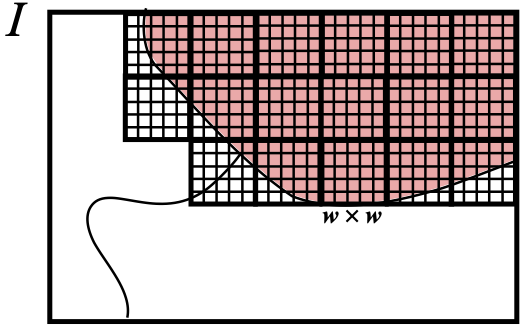
\includegraphics[width=0.4\linewidth]{\toplevelprefix/chapters/chapter3/figs/image-segmentation-tiles.png}
	\caption{Image patches with a size of $w\times w$ pixels.}
	\label{fig:image-patch}
\end{figure}

\begin{figure}[th]
	\centering
	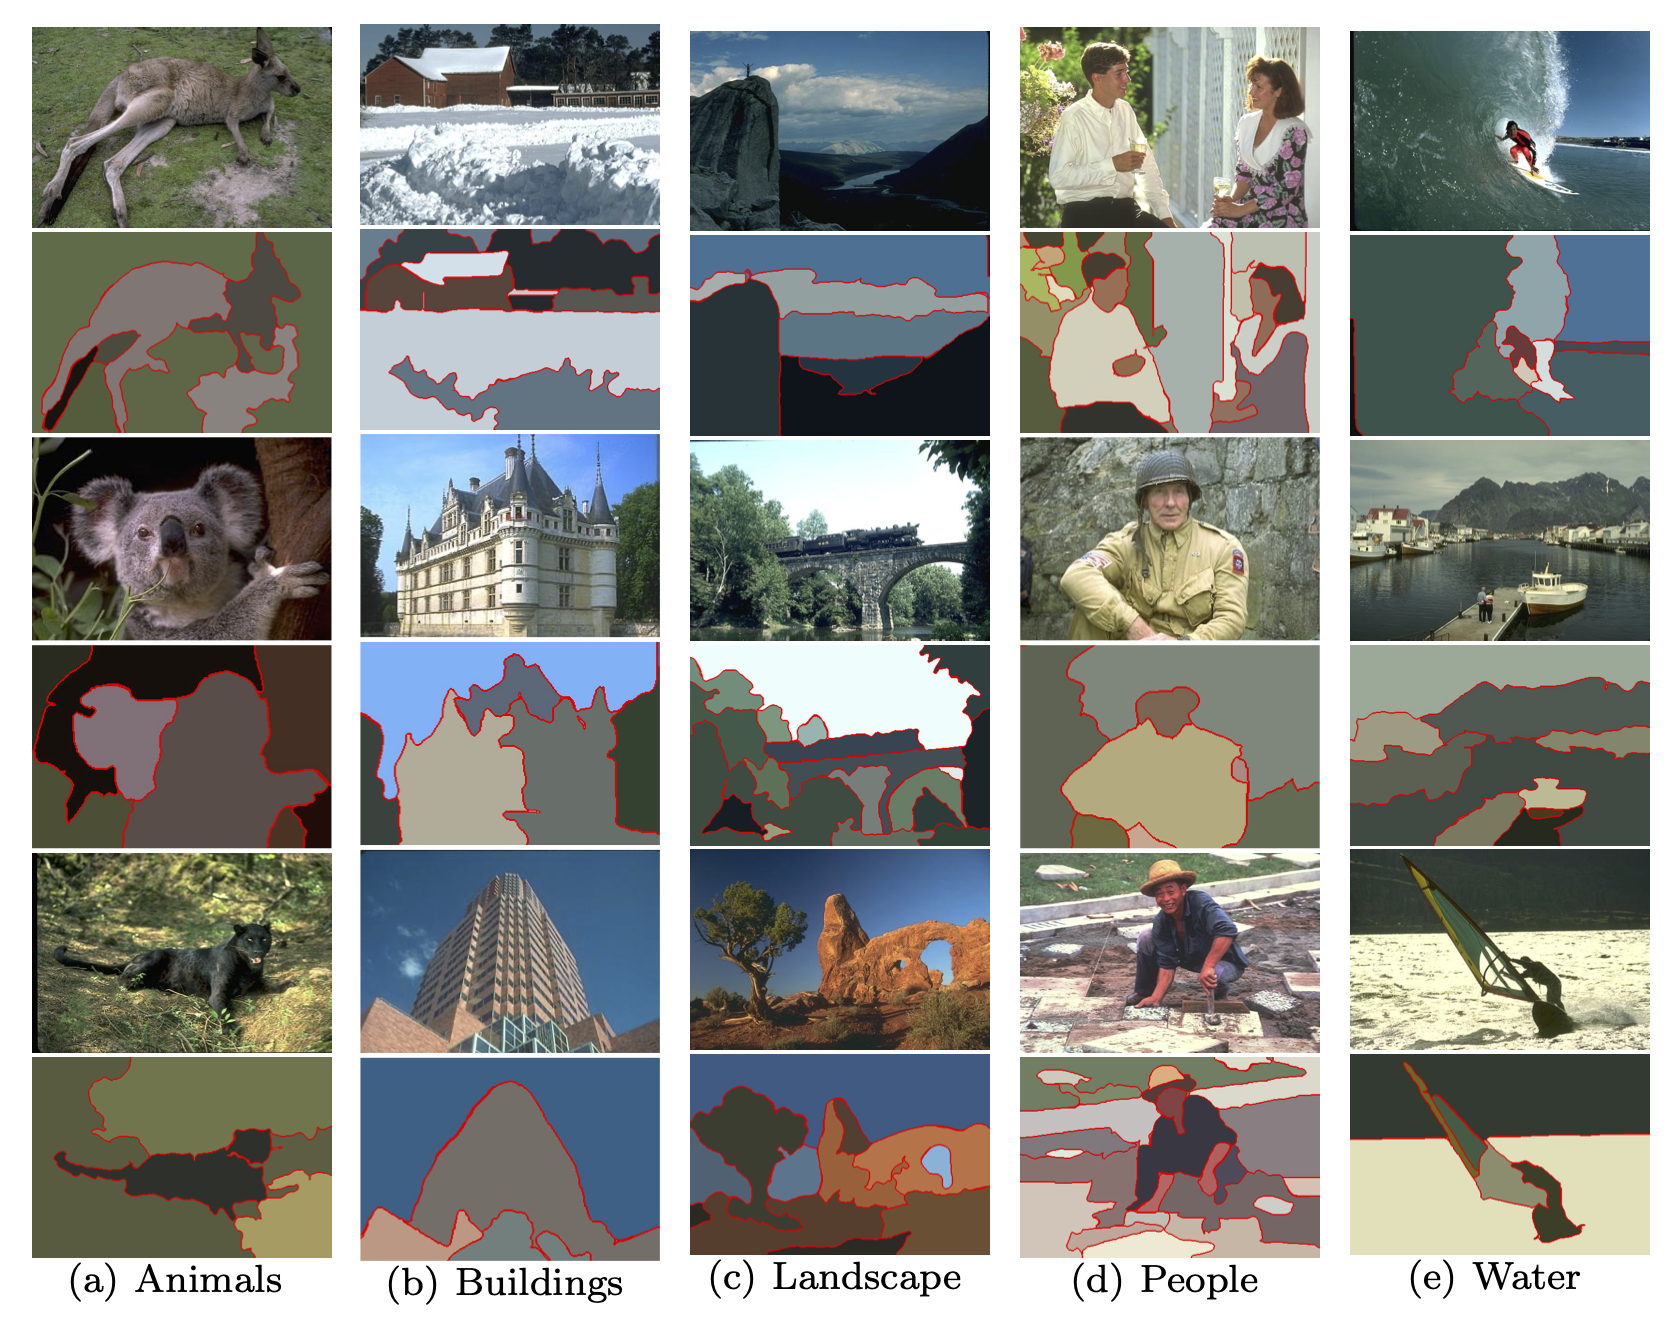
\includegraphics[width=0.8\linewidth]{\toplevelprefix/chapters/chapter3/figs/image-segmentation.png}
	\caption{Segmentation results based on the clustering algorithm applied to the image patches.}
	\label{fig:image-segmentation}
\end{figure}

\section{Maximizing Information Gain}
\label{sec:chap4-representation-learning-problem}

% \yaodong{TODO: Connect representation properties defined in Chapter 2. (suggested by Druv)}

% \yaodong{TODO: cut the citations to the ``Notes'' part in the later of the chapter.}

%\pw{add some sentences to connect!}

So far in this chapter, we have discussed how to identify a distribution with low-dimensional structures through the principle of compression. As we have seen from the previous two sections, computational compression can be realized through either the denoising operation or through clustering. Figure \ref{fig:Gaussian-Subspaces} illustrates this concept with our favorite example.
\begin{figure}[t]
    \centering
    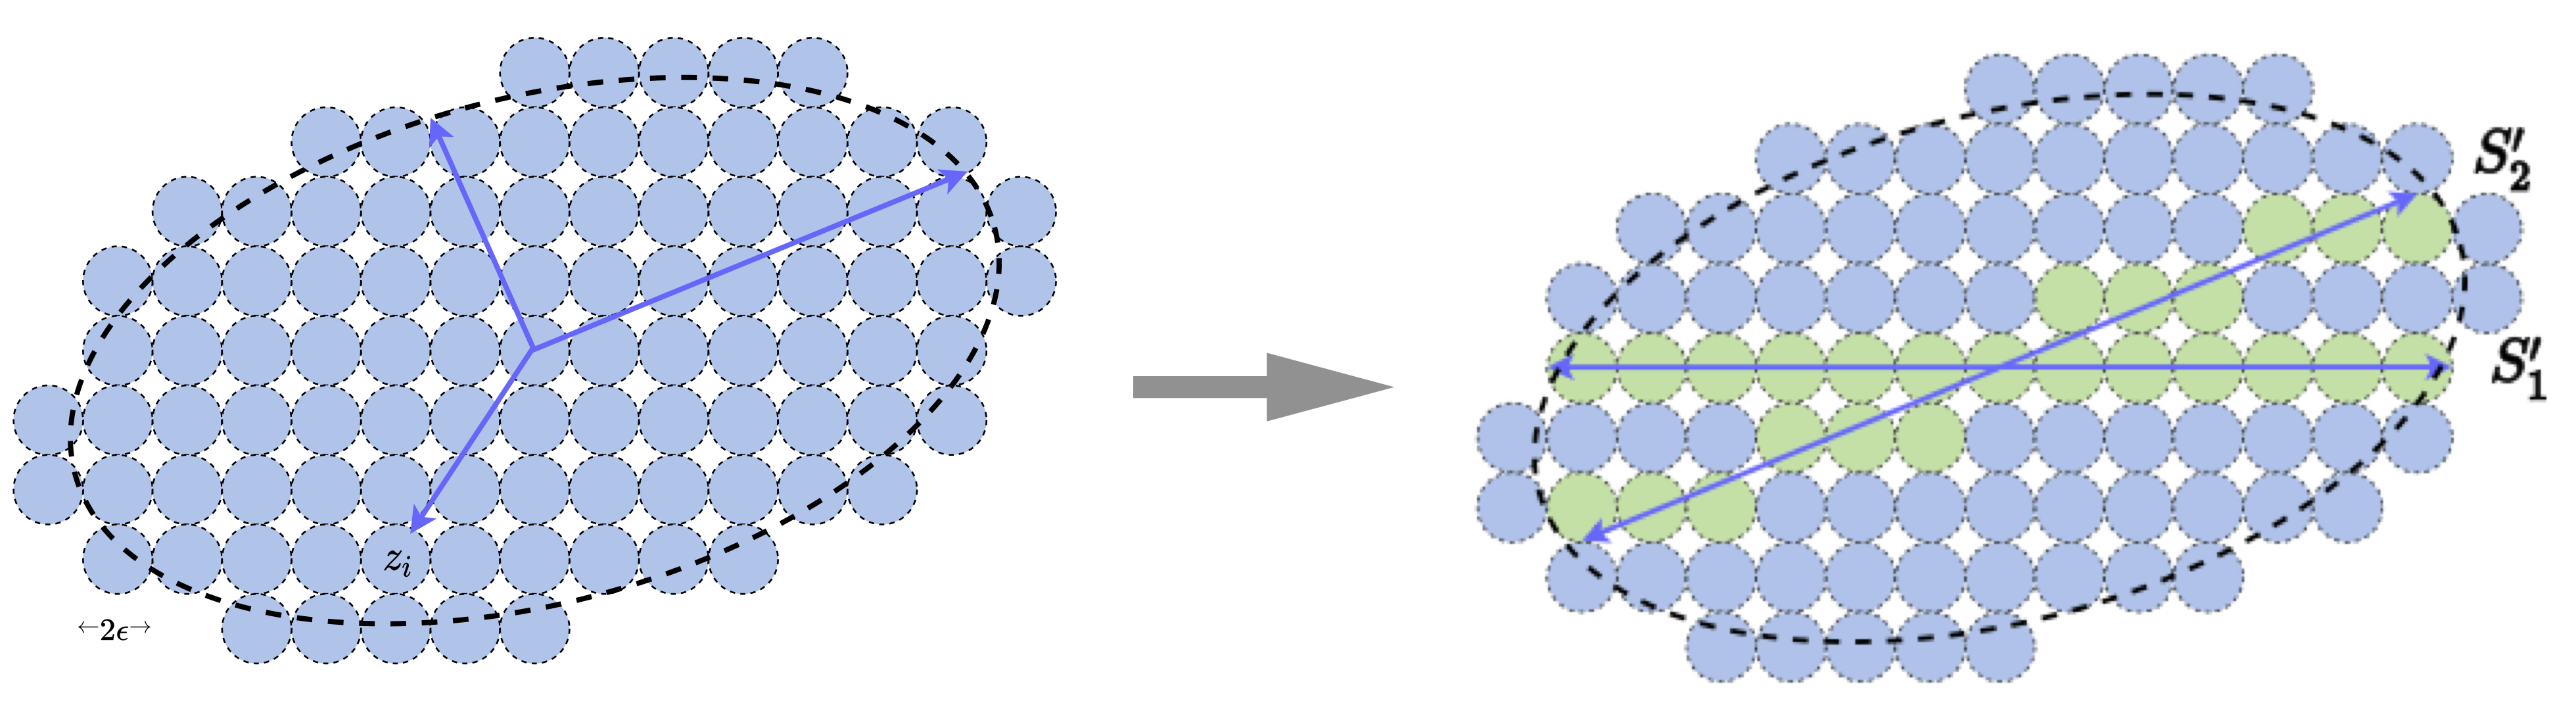
\includegraphics[width=0.8\linewidth]{\toplevelprefix/chapters/chapter3/figs/Gaussian-Subspaces.png}
    \caption{Identify a low-dimensional distribution with two subspaces (left) via denoising or clustering, starting from a generic random Gaussian distribution (right).}
    \label{fig:Gaussian-Subspaces}
\end{figure}
Of course, the ultimate goal for identifying a data distribution is to use it to
facilitate certain subsequent tasks such as segmentation, classification, or
generation (of images). Hence, how the resulting distribution is ``represented''
matters tremendously with respect to how information related to these subsequent tasks can be efficiently and effectively retrieved and utilized. This naturally raises a fundamental question: {\em what makes a representation truly ``good'' for downstream use?} In the following, we will explore the essential properties that a meaningful and useful representation should possess, and how these properties can be explicitly characterized and pursued via maximizing information gain.  

% In recent years, deep learning has seen tremendous empirical success in processing
% and modeling massive amounts of high-dimensional and multi-modal data. Much of this success has been attributed to deep networks' ability in effectively learning  ``good representations'' that facilitate many downstream tasks, e.g., classification, recognition and segmentation, and generation of visual data.

\paragraph{How to measure the goodness of representations.}
% To state the common problem behind all these practices more formally, 
One may view a given dataset as samples of a random vector $\x$ with a certain distribution in a high-dimensional space, say $\mathbb{R}^D$. Typically, the distribution of $\x$ has a much lower intrinsic dimension than the ambient space. Generally speaking,  {\em learning a representation} refers to learning a continuous mapping, say $f(\cdot)$, that transforms $\x$ to a so-called {\em feature vector} $\z$ in another (typically lower-dimensional) space, say $\mathbb{R}^d$, where $d < D$. It is hopeful that through such a mapping
\begin{equation}
	\x \in \mathbb{R}^D \xrightarrow{\hspace{2mm} f(\x)\hspace{2mm}} \z  \in \mathbb{R}^d,
	\label{eqn:chap4-1-encoding}
\end{equation}
the low-dimensional intrinsic structures of $\x$ are identified and represented by $\z$ in a more compact and structured way so as to facilitate subsequent tasks such as classification or generation. The feature $\z$ can be viewed as a (learned) compact code for the original data $\x$, so the mapping $f$ is also called an \textit{encoder}.
The fundamental question of representation learning is
\begin{center}
	\noindent{\em What is a principled and effective measure for the goodness of representations?}
\end{center}

Conceptually, the quality of a representation $\z$ depends on how well it identifies the most relevant and sufficient information of $\x$ for subsequent tasks and how efficiently it represents this information.
For a long time, it was believed and argued that the ``sufficiency'' or ``goodness'' of a learned feature representation should be defined in terms of a specific task. For example, $\z$ just needs to be sufficient for predicting the class label $\y$ in a classification problem. Below, let us start with the classic problem of image classification and argue why such a notion of a task-specific ``representation'' is limited and needs to be generalized.

%To understand the role of deep learning or deep networks in this type of representation learning, \cite{Tishby-ITW2015} proposed the \textit{information bottleneck} framework, which suggests that a measure of feature goodness is to maximize the mutual information between $\z$ and $\y$ while minimizing the mutual information between $\z$ and $\x$.

% Nevertheless, in recent years the predominant practice has been to learn first a \textit{task-agnostic} representation by pre-training a large deep neural network, in some cases known as a \textit{foundation model} \cite{Bommasani2021-vm}.
% The so-learned representation can subsequently be fine-tuned for multiple specific tasks.
% This has been shown to be more effective and efficient for many practical tasks across diverse data modalities, including speech, language, and natural images.
% Notice that representation learning in this context is different from that for a specific task, where $\z$ only needs to be good enough for predicting a specific $\y$. In a task-agnostic setting, the learned representation $\z$ needs to encode \textit{almost all essential information about the distribution of the data $\x$}. That is, the learned representation $\z$ not only is a more compact and structured representation for the intrinsic structures of $\x$, but can also recover $\x$ to a certain degree of faithfulness.
% Hence, it is natural to ask, in the task-agnostic context, what a principled measure of goodness for a learned (feature) representation should be.
% As we know, in recent practice of learning task-agnostic representations, one type of deep architectures, known as transformers \cite{vaswani2017attention}, have emerged as an almost universal choice for the backbone of deep networks, for either discriminative or generative tasks, from language to vision.
% %We will provide more details on how to derive transformer-like architecture via a white-box approach in Section~\ref{sec:chap4-white-box-transformer}.
% As we will see in this chapter, clarifying the principled measure for feature goodness is also the key to fully understand why a transformer-like architecture is suitable for task-agnostic pretraining, as well as to reveal the precise role and function of each layer in transformer-like deep networks.


% \subsection{Principles and Objectives for Representation Learning}


% TODO: compression and sparsity.

% \subsection{Deep Network Architectures: Nonlinear to Linear}


% \section{White-box Deep Networks via Unrolling}\label{sec:chap4-white-box-model-via-unrolling}

% \subsection{LISTA - Sparsity}

% \subsection{ReduNet - Compression}

% \subsection{CRATE - Compression \& Sparsity}



\subsection{Linear Discriminative Representations}\label{subsec:LDR}
%{\color{red} Outline: Introducing and formulating the principle of {\em information gain} or {\em rate reduction}. Transform the data distribution to maximize information gain. More specifically rate reduction in the important case of mixture of low-rank Gaussians.}

Suppose that $\bm{x} \in \mathbb{R}^D$ is a random vector drawn from a mixture of $K$ (component) distributions  $\mathcal{D} = \{\mathcal{D}_k\}_{k=1}^K$. Give a finite set of i.i.d. samples $\X = [\x_1, \x_2, \ldots, \x_N] \in \Re^{D\times N}$ of the random vector $\bm x$, we {\em seek a good representation}  through a continuous mapping $f(\x): \mathbb{R}^D \rightarrow \mathbb{R}^d$ that captures intrinsic structures of $\x$ and best facilitates the subsequent classification task.\footnote{Classification is the domain where deep learning demonstrated the initial success, sparking the explosive interest in deep networks. Although our study focuses on classification, we believe the ideas and principles can be naturally generalized to other settings, such as regression.} To ease the task of learning distribution $\mathcal{D}$, in the popular supervised classification setting, a true class label (or a code word for each class), usually represented by a one-hot vector $\y_i \in \mathbb{R}^K$, is given for each sample $\x_i$.

 

% Given a random vector $\bm{x} \in \mathbb{R}^D$ that is drawn from a mixture of $k$ (component) distributions  $\mathcal{D} = \{\mathcal{D}^j\}_{j=1}^k$, one of the most fundamental problems is how to effectively and efficiently {\em learn the underlying distribution} from a finite set of i.i.d. samples, say $\X = [\x_1, \x_2, \ldots, \x_N] \in \Re^{D\times N}$. 
% To this end, we {\em seek a good representation}  through a continuous mapping $f(\x): \mathbb{R}^D \rightarrow \mathbb{R}^d$ that captures intrinsic structures of $\x$ and best facilitates the subsequent classification task.\footnote{Classification is where deep learning demonstrated the initial success that has catalyzed the explosive interest in deep networks. Although our study focuses on classification, we believe the ideas and principles can be naturally generalized to other settings, such as regression.} 

\paragraph{Encoding class information via cross entropy.}  Extensive studies have shown that for many practical datasets (e.g., images, audio, and natural languages), the (encoding) mapping from the data $\bm{x}$ to its class label $\bm{y}$ can be effectively modeled by training a deep network,\footnote{Here let us not worry about yet which network we should use here and why. The purpose here is to consider any empirically tested deep network. We will leave the justification of the network architectures to the next chapter.} here denoted as $$f(\x, \theta):\x \mapsto \y$$ with network parameters $\theta \in \Theta$, where $\Theta$ denotes the parameter space. For the output $f(\x, \theta)$ to match well with the label $\y$, we like to  minimize the {\em cross-entropy loss} over a training set $\{(\x_i, \y_i)\}_{i=1}^N$: 
\begin{equation}
   \min_{\theta \in \Theta} \; - \mathbb{E}[\langle \y, \log(f(\x, \theta)) \rangle] \, \approx - \frac{1}{N}\sum_{i=1}^N \langle \y_i, \log\left(f(\x_i, \theta)\right) \rangle.
   \label{chap4-eqn:cross-entropy}
\end{equation}
The optimal network parameters $\theta $ is typically found by optimizing the above objective through an efficient gradient descent scheme, with gradients computed via back propagation (BP), as described in Section \ref{app:BP-section} of Appendix \ref{app:optimization}.

Despite its effectiveness and enormous popularity, there are two serious limitations with this approach:  1) It aims only to predict the labels $\y$ even if they might be mislabeled. Empirical studies show that deep networks, used as a ``black box,'' can even fit random labels~\cite{zhang2017understanding}.
2) With such an end-to-end data fitting,
despite plenty of empirical efforts in trying to interpret the so-learned
features, %~\cite{Zeiler-ECCV2014},
it is not clear to what extent the intermediate features learned by the network capture the intrinsic structures of the data that make meaningful classification possible in the first place. The precise geometric and statistical properties of the learned features are also often obscured, which leads to the lack of interpretability and subsequent performance guarantees (e.g., generalizability, transferability, and robustness, etc.) in deep learning.
Therefore, {\em one of the goals of this section is to address such limitations by reformulating the objective towards learning explicitly meaningful and useful representations for the data $\x$, not limited to classification.}

\begin{figure}
	\centering
	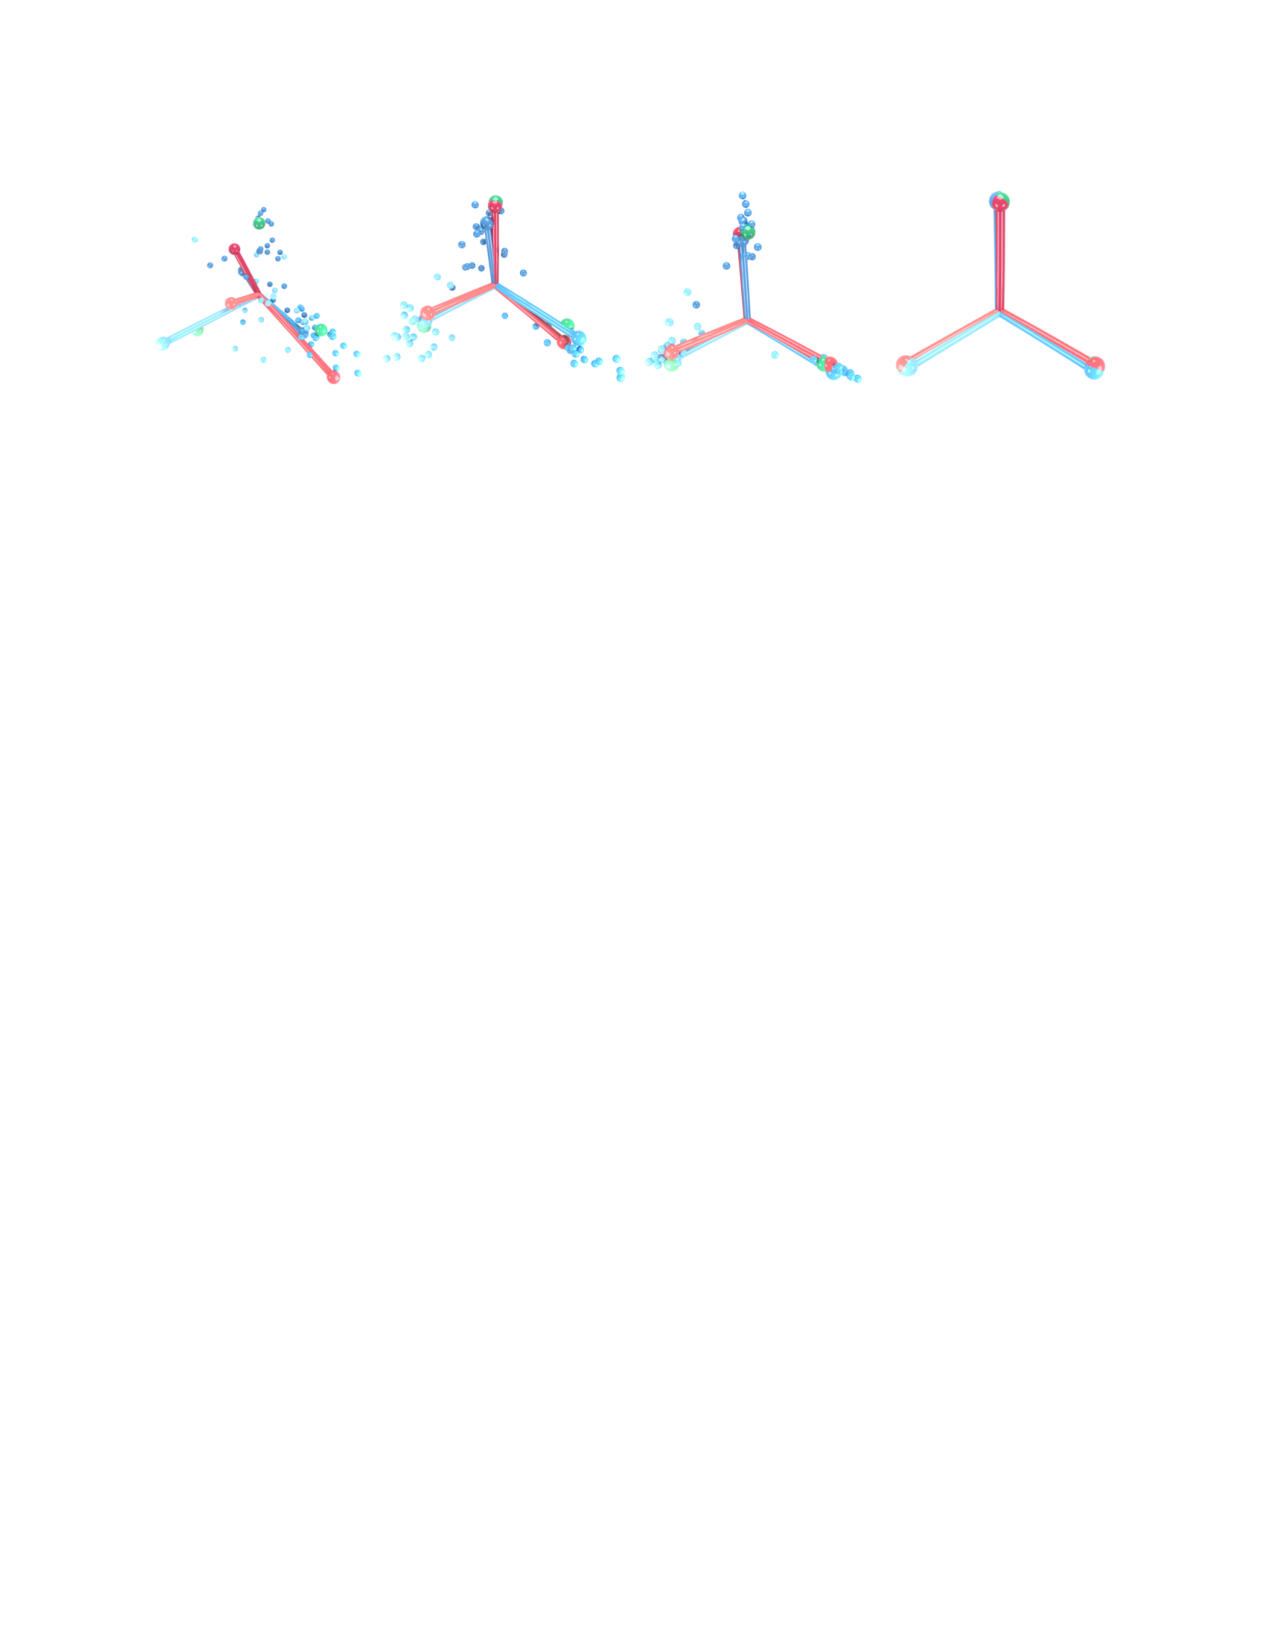
\includegraphics[width=0.95\linewidth]{\toplevelprefix/chapters/chapter3/figs/neural_collapse.pdf}
	\caption{Evolution of penultimate layer outputs of a VGG13 neural network when trained on the CIFAR10 dataset with 3 randomly selected classes. Figure from \cite{papyan2020prevalence}.}
	\label{chap4-fig:neural-collapse}
\end{figure}

\paragraph{Minimal discriminative features via information bottleneck.}
One popular approach to interpret the role of deep networks is to view outputs of intermediate layers of the network as selecting certain latent features $\z = f(\x, \theta) \in \Re^d$ of the data that are discriminative among multiple classes. Learned representations $\z$ then  facilitate the subsequent classification task for predicting the class label $\y$ by optimizing a classifier $g(\z)$:
\begin{equation}
	\x   \xrightarrow{\hspace{2mm} f(\x, \theta)\hspace{2mm}} \z  \xrightarrow{\hspace{2mm} g(\z) \hspace{2mm}} \y.
\end{equation}
We know from information theory~\cite{Cover-Thomas} that {\em the mutual information} between two random variables, say $\x,\z$, is defined to be
\begin{equation}
	I(\x; \z) = H(\x) - H(\x\mid \z),
\end{equation}
where $H(\x \vert \z)$ is the conditional entropy of $\x$ given $\z$. The mutual information is also known as {\em the information gain}: It measures how much the entropy of the random variable $\x$ can be reduced once $\z$ is given. Or equivalently, it measures how much information $\z$ contains about $\x$.  The {\em information bottleneck} (IB) formulation \cite{Tishby-ITW2015} further hypothesizes that the role of the network is to learn $\z$ as the minimal sufficient statistics for predicting $\y$. Formally, it seeks to maximize the mutual information $I(\z, \y)$
between $\z$ and $\y$ while minimizing the mutual information $I(\x, \z)$ between $\x$ and $\z$:
\begin{equation}
	\max_{\theta\in \Theta}\; \mbox{IB}(\x, \y, \z) \doteq I(\z; \y) - \beta I(\x; \z) \quad\ \mathrm{s.t.}\ \z = f(\x, \theta),
	\label{chap4-eqn:information-bottleneck}
\end{equation}
where $\beta >0$. 

Given one can overcome some caveats associated with this framework \cite{kolchinsky2018caveats-ICLR2018}, such as how to accurately evaluate mutual information with finite samples of degenerate distributions, this framework can be helpful in explaining certain behaviors of deep networks. 
For example, recent work \cite{papyan2020prevalence} indeed shows that the representations learned via the cross-entropy loss \eqref{chap4-eqn:cross-entropy} exhibit a \emph{neural collapse} phenomenon. 
That is, features of each class are mapped to a one-dimensional vector whereas all other information of the class is suppressed,  as illustrated in Figure~\ref{chap4-fig:neural-collapse}.
% % \footnote{Essentially, once an over-parameterized network fits the training data, regularization (such as weight decay) would collapse weight components or features that are not the most relevant for fitting the class labels. Besides the most salient feature, informative and discriminative features that also help define a class can be suppressed.} 
% where within-class variability and structural information are getting suppressed and ignored, as illustrated in Figure~\ref{chap4-fig:neural-collapse}. 
\begin{remark}
    Neural collapse refers to a phenomenon observed in deep neural networks trained for classification, where the learned feature representations and classifier weights exhibit highly symmetric and structured behavior during the terminal phase of training \cite{papyan2020prevalence,zhu2021geometric}. Specifically, within each class, features collapse to their class mean, and across classes, these means become maximally separated, forming a simplex equiangular configuration. The linear classifier aligns with the class mean up to rescaling. Additionally, the last-layer classifier converges to choosing whichever class has the nearest train class mean. Neural collapse reveals deep connections between optimization dynamics, generalization, and geometric structures arising in supervised learning.  
\end{remark}

From the above example of classification, we see that the so-learned representation gives a very simple encoder that essentially maps each class of data to only one code word: the one-hot vector representing each class. From the lossy compression perspective, such an encoder is too lossy to preserve information in the data distribution. Other information, such as that useful for tasks such as image generation, is severely lost in such a supervised learning process. To remedy this situation, we want to learn a different encoding scheme such that the resulting feature representation can capture much richer information about the data distribution, not limited to that useful for classification alone.

% Here by being task-dependent (depending on the label $\y$) and seeking a {\em minimal} set of most informative features for the task at hand (for predicting the label $\y$ only), the so learned network may sacrifice robustness in case the labels can be corrupted or transferability when we want to use the features for different tasks. To address this, we

% {\em the framework -- we will present in this chapter -- uses the label $\y$ as only side information to assist learning discriminative yet diverse (not minimal) representations; these representations optimize a different intrinsic objective based on }

\begin{figure}[ht]
	\centering
	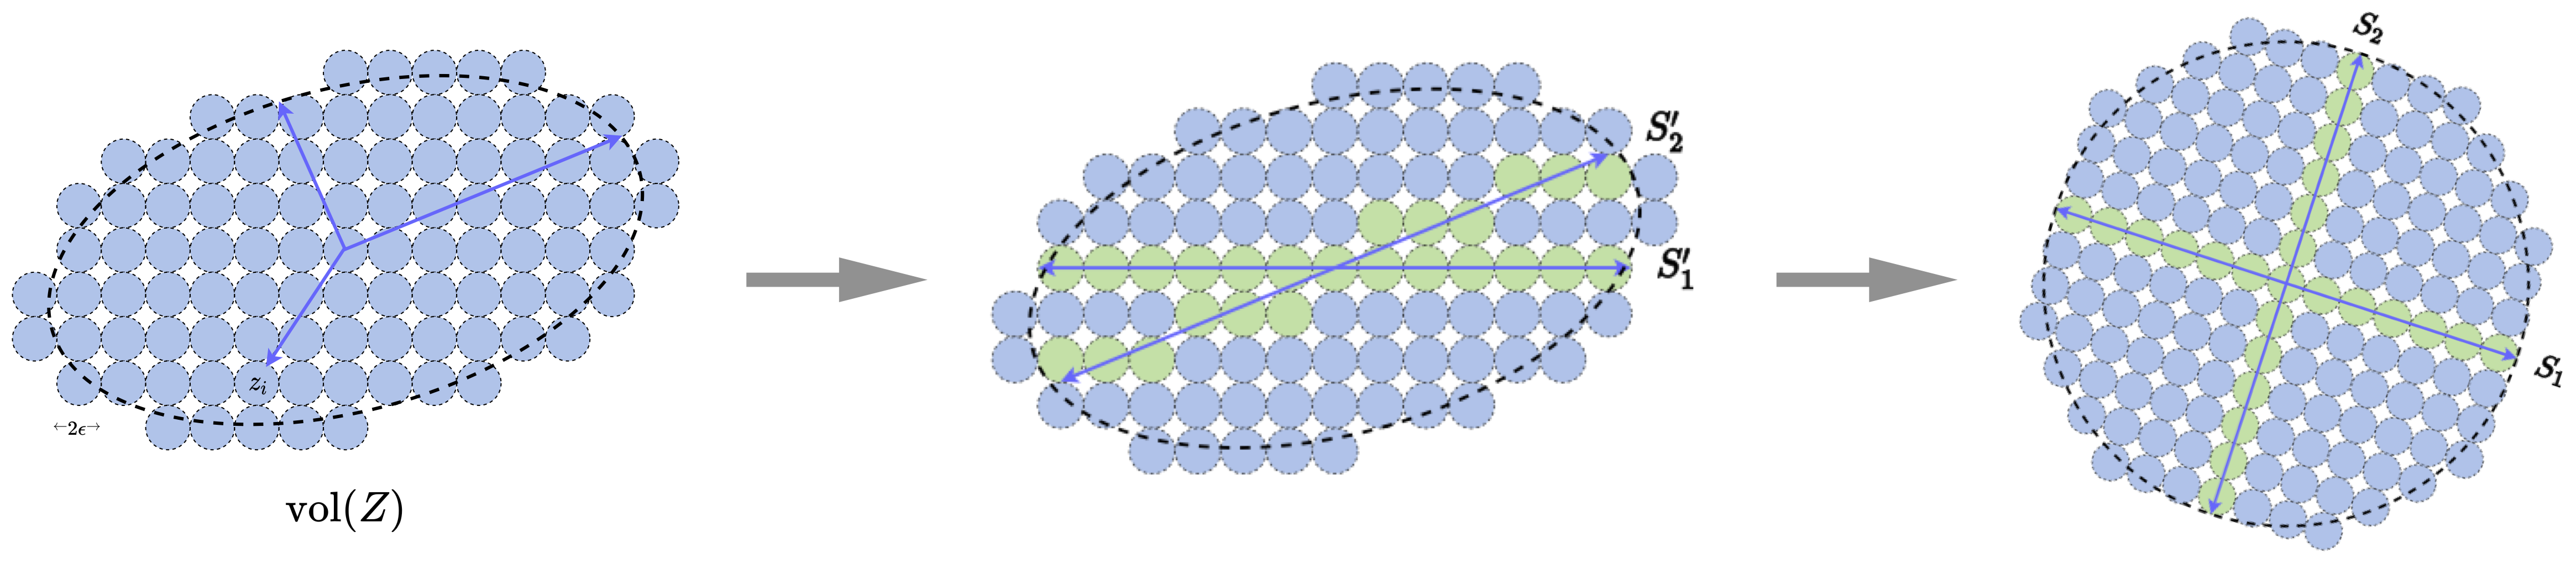
\includegraphics[width=0.99\linewidth]{\toplevelprefix/chapters/chapter3/figs/Expansion2.png}
	\caption{After identifying the low-dimensional data distribution, we would like to further transform the data distribution to a more informative structure representation: $R$ is the number of $\epsilon$-balls covering the whole space and $R^c$ is the sum of the numbers for all the subspaces (the green balls). $\Delta R$ is their difference (the number of blue balls). }\label{fig:sphere-packing}
	\label{fig:informative-representation}
\end{figure}


\paragraph{Linear discriminative representations.}
Whether the given data $\X$ of a mixed distribution $\mathcal{D}$ can be effectively classified or clustered depends on how separable (or discriminative) the component distributions $\mathcal{D}_k$ are (or can be made). One popular working assumption is that the distribution of each class has relatively {\em low-dimensional} intrinsic structures. Hence we may assume that the distribution $\mathcal{D}_k$ of each class has a support on a low-dimensional submanifold, say $\mathcal{M}_k$ with dimension $d_k \ll D$, and the distribution $\mathcal D$ of $\x$ is supported on the mixture of those submanifolds, $\mathcal M = \cup_{k=1}^K \mathcal{M}_k$,  in the high-dimensional ambient space $\Re^D$.

Not only do we need to identify the low-dimensional distribution, but we also want to represent the distribution in a form that best facilitates subsequent tasks such as classification, clustering, and conditioned generation (as we will see in the future). To do so, we require our learned feature representations to have the following properties:
\begin{enumerate}
	\item {\em Within-Class Compressible:} Features of samples from the same class should be strongly {\em correlated} in the sense that they belong to a low-dimensional linear subspace.
	\item {\em Between-Class Discriminative:} Features of samples from different classes should be highly {\em uncorrelated} and belong to different low-dimensional linear subspaces.
	\item {\em Maximally Diverse Representation:} Dimension (or variance) of the features of each class should be {\em as large as possible} as long as they are incoherent to the other classes.
\end{enumerate}
We refer to such a representation the {\em linear discriminative representation} (LDR). Notice that the first property aligns well with the objective of the classic  {\em principal component analysis} (PCA) that we have discussed in Chapter \ref{sub:pca}. The second property resembles that of the classic {\em  linear discriminant analysis} (LDA)~\cite{HastieTiFr09}. Figure \ref{fig:informative-representation} illustrates these properties with a simple example when the data distribution is actually a mixture of two subspaces. Through compression (denoising or clustering), we first identify that the true data distribution is a mixture of two low-dimensional subspaces (middle) instead of a generic Gaussian distribution (left). We then would like to transform the distribution so that the two subspaces eventually become mutually incoherent/independent (right). 

\begin{remark}
    Linear discriminant analysis (LDA)~\cite{HastieTiFr09} is a supervised dimensionality reduction technique that aims to find a linear projection of data that maximizes class separability. Specifically, given labeled data, LDA seeks a linear transformation that projects high-dimensional inputs onto a lower-dimensional space where the classes are maximally separated. Note that PCA is an unsupervised method that projects data onto directions of maximum variance without considering class labels. While PCA focuses purely on preserving global variance structure, LDA explicitly exploits label information to enhance discriminative power; see the comparison in \Cref{fig:LDA}. 
\end{remark}

\begin{figure}
	\centering
	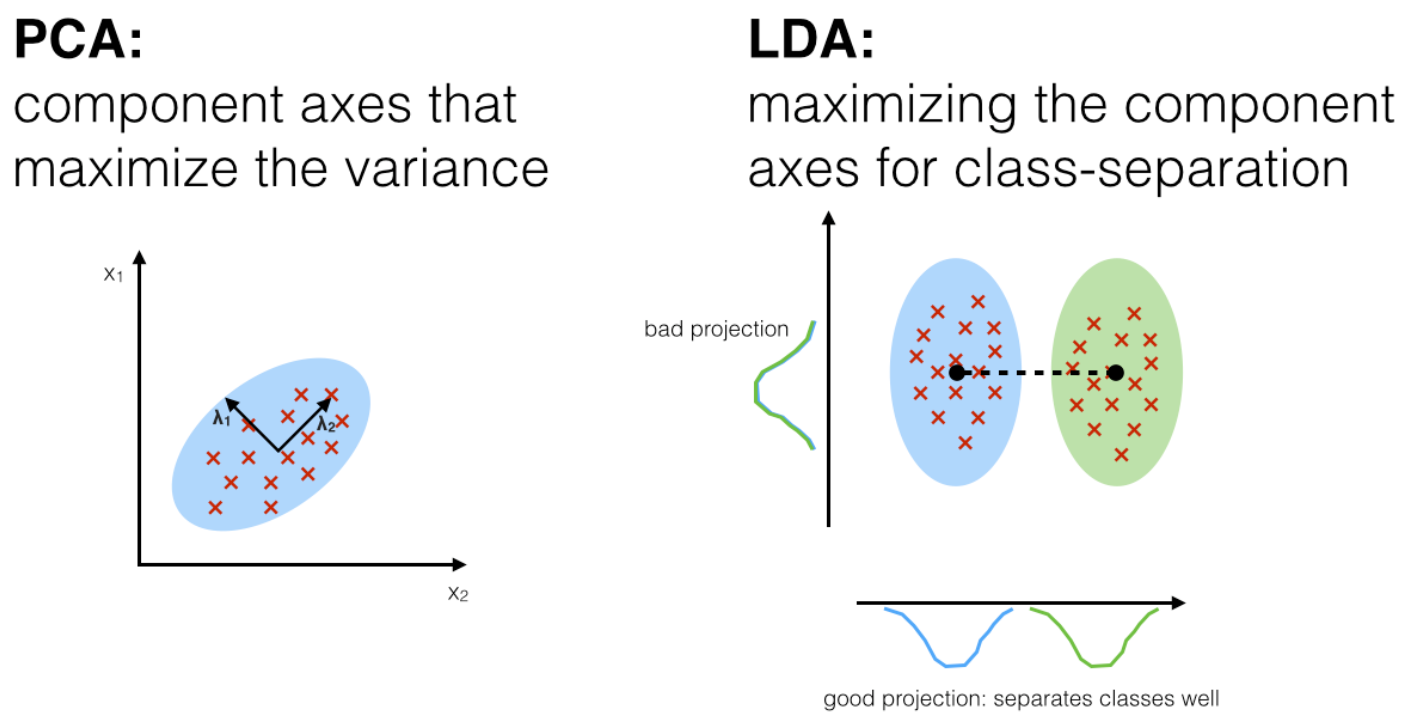
\includegraphics[width=0.7\linewidth]{\toplevelprefix/chapters/chapter3/figs/LDA.png}\vspace{-0.1in}
	\caption{Comparison between PCA and LDA. Figures adpoted from \url{https://sebastianraschka.com/Articles/2014_python_lda.html}.}
	\label{fig:LDA}
\end{figure}


The third property is also important because we want the learned features to reveal all possible causes of why one class is different from all other classes. For example, to tell ``apple'' from ``orange'', we care not only about color but also shape and the leaves. Ideally, the dimension of each subspace $\{\mathcal{S}_k\}$ should be equal to that of the corresponding submanifold $\mathcal{M}_k$. This property will be important if we would like the map $f(\x,\theta)$ to be {\em invertible} for tasks such as image generation. For example, if we draw different sample points from the feature subspace for ``apple'', we should be able to decode them to generate diverse images of apples. The feature learned from minimizing the cross entropy \eqref{chap4-eqn:cross-entropy} clearly does not have this property.


In general, although the intrinsic structures of each class/cluster may be low-dimensional, they are by no means simply linear (or Gaussian) in their original representation $\x$ and they need to be made linear first, through some nonlinear transformation.\footnote{We will discuss how this can be done explicitly in Chapter \ref{ch:autoencoding}.} Therefore, overall, we use the nonlinear transformation $f(\x,\theta)$ to seek a representation of the data such that the subspaces that represent all the classes are maximally incoherent linear subspaces. To be more precise, we want to learn a mapping {$\z = f(\x,\theta)$} that maps each of the submanifolds $\mathcal{M}_k \subset \Re^D$ (Figure~\ref{chap4-fig:mcr-diagram} left) to a {\em linear} subspace $\mathcal{S}_k \subset \Re^d$ (Figure~\ref{chap4-fig:mcr-diagram} right). To some extent, the resulting multiple subspaces $\{\mathcal{S}_k\}$ can be viewed as discriminative {\em generalized principal components} \cite{GPCA} or, if orthogonal, {\em independent components} \cite{hyvarinen2000independent} of the resulting features $\z$ for the original data $\bm x$.
As we will see in the next Chapter \ref{ch:representation}, deep networks precisely play the role of modeling and realizing this nonlinear transformation from the data distribution to linear discriminative representations.


%\subsection{The Principle of Maximal Information Gain}
\subsection{The Principle of Maximal Coding Rate Reduction}\label{subsec:MCR2}



%\paragraph{Classic  Information Gain.}  The classic  {\em Information Gain} (IG), which aims to maximize the reduction of entropy of a random variable, say $\bm z$, with respect to an observed attribute, say $\bm \pi$:$\max_{\bm \pi} \; \mbox{IG}(\bm z, \bm \pi) \doteq H(\bm z) - H(\bm z \mid \bm \pi),$i.e., the {\em mutual information} between $\z$ and $\bm \pi$ \cite{Cover-Thomas}. Maximal information gain has been widely used in areas such as decision trees \cite{decision-trees}. However, MCR$^2$ is used differently in several ways: 1) A typical setting of MCR$^2$ is when the data class labels are given, i.e. $\bm \Pi$ is known, MCR$^2$ focuses on learning representations $\bm z(\theta)$ rather than fitting labels. 2) In traditional settings of IG, the number of attributes in $\bm z$ cannot be so large and their values are discrete (typically binary). Here, the ``attributes'' $\bm \Pi$  represent the probability of a multi-class partition for all samples and their values can even be continuous. 3) As mentioned before, entropy $H(\bm z)$ or mutual information $I(\bm z, \bm \pi)$ \cite{hjelm2018learning} is not well-defined for degenerate continuous distributions whereas the rate distortion $R(\bm z, \epsilon)$ is and can be accurately and efficiently computed for (mixed)  subspaces, at least.


Although the three properties---{\em between-class discriminative}, {\em
within-class compressible}, and {\em maximally diverse representation}---for linear discriminative representations (LDRs) are all highly desired properties  of the learned representation $\z$, they are by no means easy to obtain: Are these properties compatible so that we can expect to achieve them all at once? If so, is there a {\em simple but principled} objective that can measure the goodness of the resulting representations in terms of all these properties? The key to these questions {is to find} a principled ``measure of compactness'' or ``information gain''  for the distribution of a random variable $\z$ or from its finite samples $\{\bm z_i\}_{i=1}^N$. Such a measure should directly and accurately characterize intrinsic geometric or statistical properties of the distribution, in terms of its intrinsic dimension or {volume}. Unlike the cross entropy \eqref{chap4-eqn:cross-entropy} or information bottleneck \eqref{chap4-eqn:information-bottleneck}, such a measure should not depend exclusively on class labels so that it can work in more general settings such as supervised, self-supervised, semi-supervised, and unsupervised settings.

\begin{figure}
	\centering
	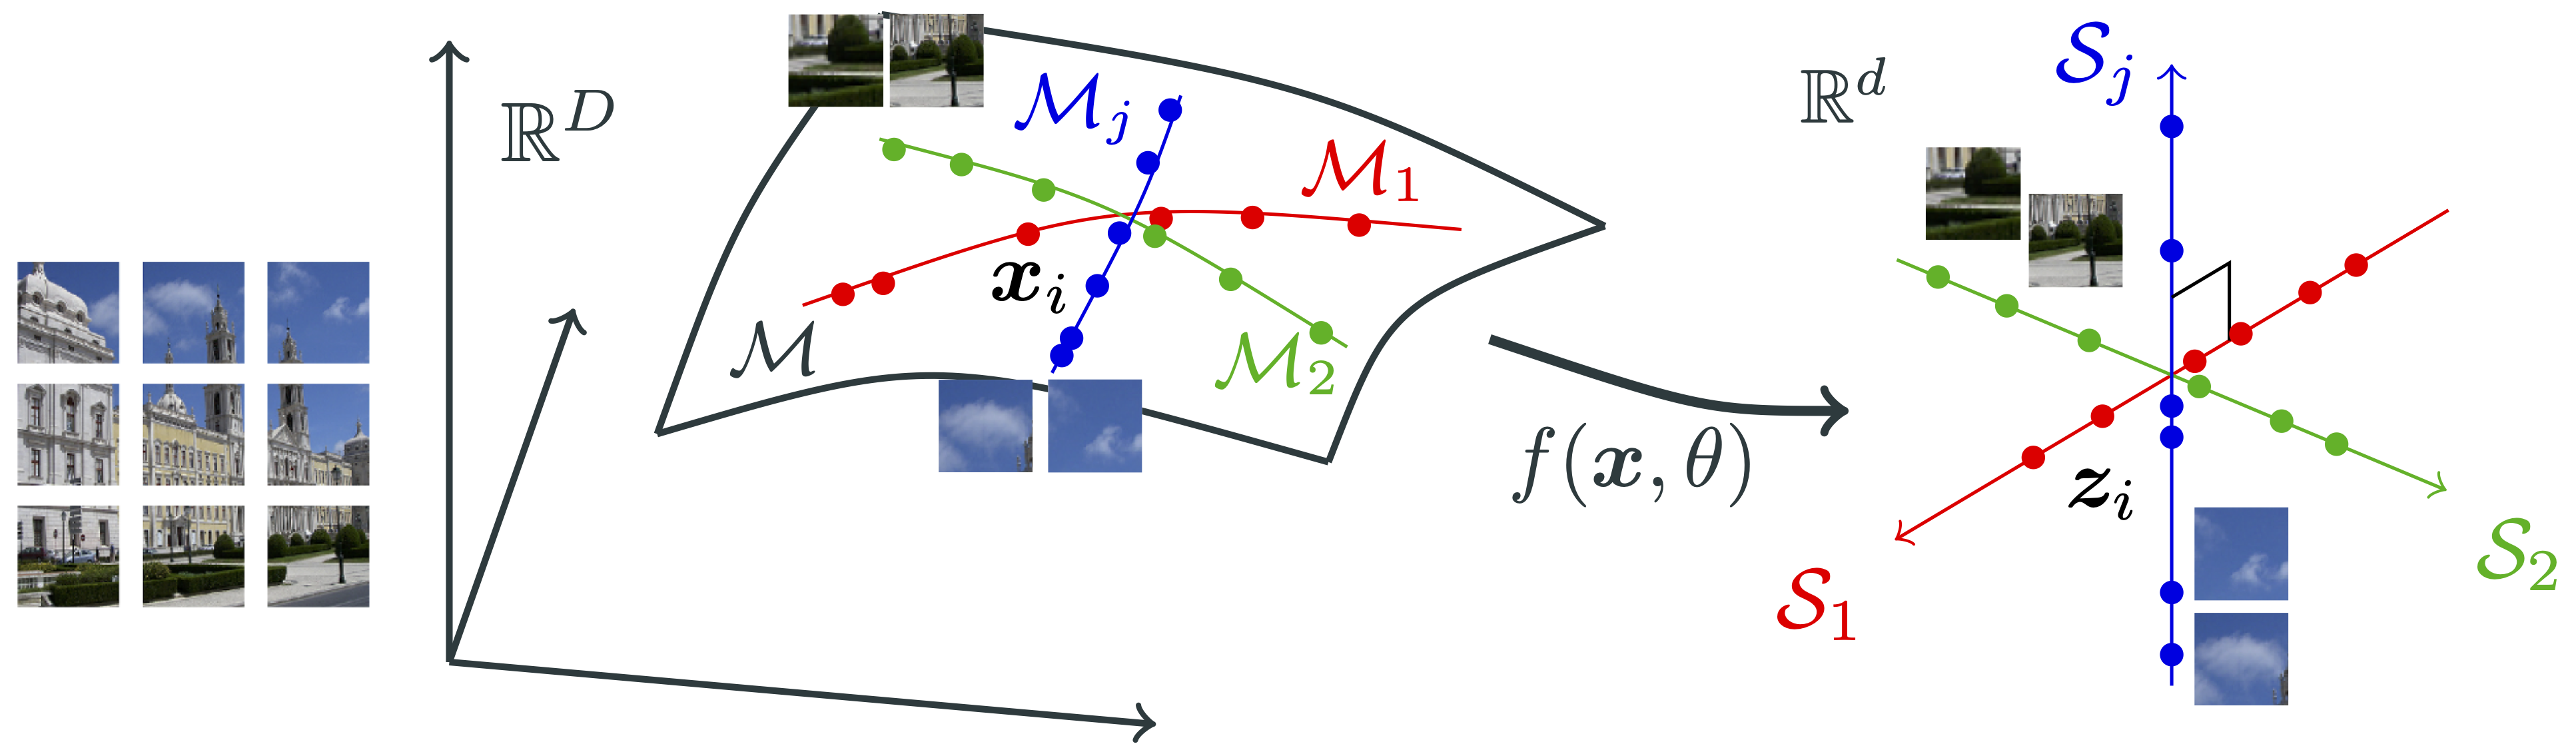
\includegraphics[width=0.8\linewidth]{\toplevelprefix/chapters/chapter3/figs/mcr_diagram.png}
	\caption{The distribution $\mathcal D$ of high-dimensional data $\x\in \Re^D$ is supported on  a manifold $\mathcal{M}$ and its classes on low-dimensional submanifolds $\mathcal{M}_k$. We aim to learn a mapping $f(\x, \theta)$ parameterized by $\theta$ such that $\z_i = f(\x_i, \theta)$ lie on a union of maximally uncorrelated subspaces $\{\mathcal{S}_k\}$.}
	\label{chap4-fig:mcr-diagram}
\end{figure}
% As we discussed above, we would like the learned representation to preserve as much information about $\x$. If so, one can approximately recover $\x$ from the corresponding $\z$. In other words, there exists a decoding map $g(\z)$ such that
% \begin{equation}
%     \x   \xrightarrow{\hspace{2mm} f(\x)\hspace{2mm}} \z  \xrightarrow{\hspace{2mm} g(\z) \hspace{2mm}} \hat{\x},
% \end{equation}
% where $\hat{\x}$ closely approximates $\x$. Hence we would like to maximize the mutual information between $\x$ and $\hat \x$ while we want $\z$ to be as compact as possible. A natural measure of compactness for $\z$ is its entropy $H(\z)$. We want it to be minimized. Therefore, we could argue that to seek a good representation, we would like to maximize the following objective:
% \begin{equation}
%     \max I(\x, \hat{\x}) - \alpha H(\z).
%     \label{eqn:info-gain-obj1}
% \end{equation}
% Notice that $I(\x, \hat{\x}) \ge R(\hat \x,\epsilon)$ if the decoded $\hat \x$ satisfies $\mathbb E[\|\x - \hat \x \|_2] \le \epsilon$. Hence the above objective can be replaced as
% \begin{equation}
%     \max R(\hat \x,\epsilon) - \alpha H(\z).
%     \label{eqn:info-gain-obj2}
% \end{equation}

% However, differential entropy $H(\z)$ is not well-defined for continuous random variables with degenerate distributions.  This is unfortunately the case here for $\z$. In this case, strictly speaking $H(\z)$ can be negative infinity, as we can see from the differential entropy of a (nearly degenerate) Gaussian distribution in \eqref{eqn:entropy-Gaussian-multi}. To alleviate this difficulty, as we have discussed earlier in this chapter, we may use another measure of ``compactness'' of a distribution, the {\em rate distortion}: Recall that, given a random variable $\z$ and a prescribed precision $\epsilon >0$, the rate distortion $R(\z, \epsilon)$ is the minimal number of binary bits needed to encode $\z$ such that the expected decoding error is less than $\epsilon$, i.e., the decoded $\hat \z$ satisfies $\mathbb E[\|\z - \hat \z \|_2] \le \epsilon$. Hence the above objective \eqref{eqn:info-gain-obj2} can be replaced as:
% \begin{equation}
%     \max R(\hat \x,\epsilon) - \alpha R(\z, \epsilon).
%     \label{eqn:info-gain-obj3}
% \end{equation}




%To learn a discriminative linear representation for intrinsic low-dimensional structures from high-dimensional data, we here propose an information-theoretic measure that maximizes the coding rate difference between the whole dataset and the sum of each individual class, known as {\em rate reduction}. This new objective provides a more unifying view of the above objectives such as cross-entropy, information bottleneck, and contractive and contrastive learning. {\em We will rigorously show that when the intrinsic dimensions of the submanifolds are known and this objective is optimized, the resulting representation indeed has the desired properties listed above.}


% However, entropy is not well-defined for continuous random variables with degenerate distributions. The same difficulty resides with evaluating mutual information $I(\x, \z)$ for degenerate distributions.
% This is unfortunately the case here.
% To alleviate this difficulty, as we have discussed earlier in this chapter, we may use another measure of ``compactness'' of a distribution, the {\em rate distortion}:
% Given a random variable $\z$ and a prescribed precision $\epsilon >0$, the rate distortion $R(\z, \epsilon)$ is the minimal number of binary bits needed to encode $\z$ such that the expected decoding error is less than $\epsilon$, i.e., the decoded $\hat \z$ satisfies $\mathbb E[\|\z - \hat \z \|_2] \le \epsilon$.

%\yaodong{TODO: change the notion for $i$-th sample from $\bm{z}_{i}$ to $\bm{z}^{i}$, since $\bm{z}_{\ell}^{i}$ denotes the $i$-th sample at the $\ell$-th layer.}

Without loss of generality, assume that the distribution $\mathcal D$ of the random vector $\x$ is supported on a mixture of distributions, i.e., $\mathcal D = \cup_{k=1}^K \mathcal{D}_k$,  where each $\mathcal{D}_k \subset \Re^D$ has a low intrinsic dimension in the high-dimensional ambient space $\Re^D$. Let $\bm X_k \in \Re^{D\times N_k}$ denote the data matrix whose columns are samples drawn from the distribution $\mathcal{D}_k$, where $N_k$ denotes the number of samples for each $k=1,\dots,K$. Then, we use $\bm X=[\bm X_1,\dots,\bm X_K] \in \Re^{D\times N}$ to denote all the samples, where $N=\sum_{k=1}^K N_k$. 
%Suppose that we have a set of samples $\X = \cup_{j=1}^k \X_j$ drawn from the distribution $\mathcal D$, where $\X_j$ contains samples drawn from the corresponding distribution $\mathcal{D}_j$ for each $j=1,\dots,k$. 
Recall that we also use $\vx_i$ to denote the $i$-th sample of $\X$, i.e., $\X=[\vx_1,\dots,\vx_N] $. Under an encoding mapping:
\begin{equation}
	\x   \xrightarrow{\hspace{2mm} f(\x)\hspace{2mm}} \z,
\end{equation}
the input samples are mapped to $\vz_i = f(\vx_i)$ for each $i=1,\dots,N$. With an abuse of notation, we also write $\Z_k = f(\X_k)$ and $\Z = f(\X)$. Therefore, we have $\Z = [\bm Z_1,\dots,\bm Z_K]$ and $\Z = [\vz_1,\dots\vz_N]$. 

On one hand, for learned features to be discriminative, features of different classes/clusters are preferred to be {\em maximally incoherent} to each other. Hence, they together should span a space of the largest possible volume (or dimension) and the coding rate of the whole set $\Z$ should be as large as possible. On the other hand, learned features of the same class/cluster should be highly correlated and coherent. Hence, each class/cluster should only span a space (or subspace) of a very small volume and the coding rate should be as small as possible. Now, we will introduce how to measure the coding rate of the learned features.  

\paragraph{Coding rate of features.} Notably, a practical challenge in evaluating the coding rate is that the underlying distribution of the feature representations $\Z$ is typically unknown. To address this, we may approximate the features $\Z = [\z_1, \ldots, \z_N]$ as samples drawn from a multivariate Gaussian distribution. Under this assumption, as discussed in Chapter \ref{subsec:lossy DR}, the compactness of the features $\Z$ {\em as a whole} can be measured in terms of the average coding length per sample,  referred to as the {\em coding rate}, subject to a precision level $\epsilon > 0$ (see \eqref{eqn:rate-Gaussian}) defined as follows:
\begin{equation}
	R_{\epsilon}(\Z) = \frac{1}{2}\log\det\left(\I + \frac{d}{N\epsilon^{2}}\Z\Z^{\top}\right).
	\label{chap4-eqn:coding-length-eval}
\end{equation}

On the other hand, we hope that a nonlinear transformation $f(\x)$ maps each class-specific submanifold $\mathcal{M}_k \subset \mathbb{R}^D$ to a maximally incoherent linear subspace $\mathcal{S}_k \subset \mathbb{R}^d$ such that the learned features $\Z$ lie in a union of low-dimensional subspaces. This structure allows for a more accurate evaluation of the coding rate by analyzing each subspace separately. % To this end, we partition the data $\Z$ into multiple subsets: $\Z = \Z_1 \cup \cdots \cup \Z_k$, where each subset $\Z_j$ lies within in one low-dimensional subspace. 
% The above coding rate \eqref{chap4-eqn:coding-length-eval} can then be accurately computed for each subset as follows:
% \begin{align}
%     R_{\epsilon}(\Z_j) = \frac{1}{2} \log\det\left(\I + \frac{d}{N_j\epsilon^{2}}\Z_j\Z_j^{\top}\right),
% \end{align}
% where $N_j$ denotes the number of samples in $\Z_j$. 
% For convenience, let $\bm{\Pi} = \{\bm{\Pi}^j \in \Re^{N \times N}\}_{j=1}^{k}$ be a set of diagonal matrices whose diagonal entries encode the membership of the $N$ samples in the $k$ classes. More specifically, the diagonal entry $\bm \Pi^j(i,i)$ of $\bm \Pi^j$ indicates the probability of sample $i$ belonging to subset $j$. Therefore $\bm{\Pi}$ lies in a simplex: ${\Omega} \doteq \{\bm{\Pi} \mid \bm{\Pi}^j \ge \mathbf{0}, \; \bm{\Pi}^1 + \cdots + \bm{\Pi}^k = \I\}$. 
Recall that the columns of $\Z_k$ denotes the features of the samples in $\X_k$ for each $k=1,\dots,K$. The coding rate for the features in $\bm Z_k$ can be computed as follows: 
\begin{align}
    R_{\epsilon}(\Z_k) = \frac{N_k}{2N}\log\det\left(\I + \frac{d}{N_k\epsilon^{2}}\Z_k\Z_k^{\top}\right)
\end{align}
Then, the sum of the average coding rates of features in each class is 
\begin{equation}
	 R_{\epsilon}^c(\Z) \doteq \sum_{k=1}^K R_{\epsilon}(\Z_k),
	\label{chap4-eqn:compress-loss-eval}
\end{equation}
% Note that when $\Z$ is given, $R_{\epsilon}^c(\Z \mid \bm{\Pi})$ is a concave function of $\bm{\Pi}$.
% The function $\log\det(\cdot)$ in the above expressions has been long known as an effective heuristic for rank minimization problems, with guaranteed convergence to local minimum \cite{fazel2003log-det}. {As it nicely characterizes the coding rate of Gaussian or subspace-like distributions, $\log\det(\cdot)$ can be very effective in clustering or classification of data that are mixed Gaussians \cite{ma2007segmentation}.} Note that for the clustering purpose alone, one may only care about the sign of $\Delta R$ to decide whether to partition the data or not, which leads to the greedy clustering Algorithm \ref{alg:steepest_descent_coding_length} studied in the previous section. More specifically, in the context of clustering {\em finite} samples, one needs to use the more precise measure of the coding length mentioned earlier in Section \ref{sec:clustering-Gaussians}. See \cite{ma2007segmentation} for more details.
% As discussed in Chapter \ref{subsec:lossy DR}, we can use the metric  \eqref{eq:coding rate} to measure the compactness (i.e., coding rate) for the whole set of the features and want $R_{\epsilon}(\bm Z)$ to be large. 
% Hence we want the coding rate (or length) for the whole set of features $R_{\epsilon}(\Z)$ to be large (see \eqref{chap4-eqn:coding-length-eval}). \pw{We should relate here to Chpa 3.3.3!} 
% Hence we want the coding rate for each subset $\Z_j$ to be small. We denote the sum of all these coding rates as
 % where $\bm \Pi$ denotes the partition $\Z \rightarrow \cup_{j=1}^k \Z_j$.

Therefore, a good representation $\Z$ of $\X$ is the one that achieves a large difference between the coding rate for the whole and that for all the classes:
\begin{equation}
	\Delta R_{\epsilon}(\Z) \doteq R_{\epsilon}(\Z) - R_{\epsilon}^c(\Z).
	\label{chap4-eqn:coding-length-reduction}
\end{equation}
Notice that, as per our discussions earlier in this chapter, this difference can be interpreted as the amount of ``information gained'' by identifying the correct low-dimensional clusters $\Z_k$ within the overall set $\Z$.

If we choose our feature mapping $f(\cdot)$ to be a deep neural network $f(\cdot,\theta)$ with network parameters $\theta$, the overall process of the feature representation and the resulting rate reduction  can be illustrated by the following diagram:
\begin{equation}
	\X
	\xrightarrow{\hspace{2mm} f(\x, \theta)\hspace{2mm}} \Z  \xrightarrow{\hspace{2mm} \epsilon \hspace{2mm}} \Delta R_{\epsilon}(\Z).
	\label{chap4-eqn:flow}
\end{equation}
Note that $\Delta R_{\epsilon}$ is {\em monotonic} in the scale of the features $\Z$. To ensure fair comparison across different representations, it is essential to {\em normalize the scale} of the learned features. This can be achieved by either imposing the Frobenius norm of each class $\Z_k$ to scale with the number of features in $\Z_k \in \mathbb R^{d \times N_k}$, i.e., $\|\Z_k\|_F^2 = N_k$, or by normalizing each feature to be on the unit sphere, i.e., $\z_i \in \mathbb{S}^{d-1}$, where $N_k=\mathrm{tr}(\bm \Pi_k)$ denotes the number of samples in the $k$-th class. This formulation offers a natural justification for the need for ``batch normalization'' in the practice of
training deep neural networks \cite{ioffe2015batch}. % An alternative, arguably simpler, way to normalize the scale of learned representations is to ensure that the mapping of each layer of the network is approximately {\em isometric} \cite{ISOnet}.

Once the representations are comparable, the goal becomes to learn a set of features $\Z  = f(\X, \theta)$  such that they maximize the reduction between the coding rate of all features and that of the sum of features w.r.t. their classes:
\begin{equation}
	\begin{aligned}
		\max_{\theta } & \;  \Delta R_{\epsilon}\big(\Z \big) \doteq R_{\epsilon}(\Z) - R_{\epsilon}^c(\Z ), \\
		\mbox{s.t.} & \ \ \, \Z = f(\bm X, \theta),\  \|\Z_k\|_F^2                                          = N_k,\ k=1,\dots,K. 
	\end{aligned}
	\label{eqn:maximal-rate-reduction}
\end{equation}
We refer to this as the principle of {\em maximal coding rate reduction} (MCR$^2$),
a true embodiment of Aristotle's famous quote:
\begin{quote}
	\centering
	``{\em The whole is greater than the sum of its parts.}''
\end{quote}
To learn the best representation, we require that {\em the whole is maximally greater than the sum of its parts}. Let us examine the example shown in Figure \ref{fig:informative-representation} again. From a compression perspective, the representation on the right is {\em the most compact one} in the sense that the difference between the coding rate when all features are encoded as a single Gaussian (blue) and that when the features are properly clustered and encoded as two separate subspaces (green) is maximal.\footnote{Intuitively, the ratio between the ``volume'' of the whole space spanned by all features and that actually occupied by the features is maximal.}

 
    Note that the above MCR$^2$  principle is designed for supervised learning problems, where the group memberships (or class labels) are known. However, this principle can be naturally extended to unsupervised learning problems by introducing a membership matrix, which encodes the (potentially soft) assignment of each data point to latent groups or clusters. Specifically, let $\bm \Pi = \{\bm \Pi_k\}_{k=1}^K \subset \R^{N\times N}$ be a set of diagonal matrices whose diagonal entries encode the membership of the $N$ samples into $K$ classes. That is, $\bm \Pi$ lies in a simplex $\Omega \doteq \{\bm \Pi: \bm \Pi_k \ge \bm 0: \sum_{k=1}^K \bm \Pi_k = \bm I_N\}$. Then, we can define the average coding rate with respect to the partition $\bm \Pi$ as
    \begin{align}\label{eq:MCRc}
        R_{\epsilon}^c(\Z \mid \bm \Pi) \doteq \sum_{k=1}^K \frac{\mathrm{tr}(\bm \Pi_k)}{2N}\log\det\left(\bm I + \frac{d}{\mathrm{tr}(\bm \Pi_k)\epsilon^2}\bm Z\bm \Pi_k \bm Z^\top \right).
    \end{align}
    When $\bm Z$ is given, $R_{\epsilon}^c(\Z \vert \bm \Pi)$ is a concave function of $\bm \Pi$. Then the MCR$^2$ principle for unsupervised learning problems becomes as follows:
    \begin{align}\label{eq:MCR pi}
        \max_{\bm \Pi, \theta} & \  \Delta R_{\epsilon}\big(\Z  \mid \bm \Pi) \doteq R_{\epsilon}(\bm Z) - R_{\epsilon}^c(\Z \mid \bm \Pi) \notag \\ 
       \mathrm{s.t.}  & \ \ \ \bm Z = f(\bm X, \theta),\ \|\bm Z \bm \Pi_k\|_F^2 = N_k,\ k = 1,\dots,K,\ \bm\Pi \in \Omega. 
    \end{align}
    Compared to \eqref{eqn:maximal-rate-reduction}, the formulation here allows for the joint optimization of both the group memberships and the network parameters. In particular, when $\bm \Pi$ is fixed to a group membership matrix that assigns $N$ data points into $K$ groups, Problem \eqref{eq:MCR pi} can recover Problem \eqref{eqn:maximal-rate-reduction}.
 


% \paragraph{Relationship to Classic  Information Gain.}
%  The maximal coding rate reduction can be viewed as a generalization to the classic  {\em Information Gain} (IG), which aims to maximize the reduction of entropy of a random variable, say $\bm z$, with respect to an observed attribute, say $\bm \pi$:
% $
% \max_{\bm \pi} \; \mbox{IG}(\bm z, \bm \pi) \doteq H(\bm z) - H(\bm z \mid \bm \pi),
% $
% i.e., the {\em mutual information} between $\z$ and $\bm \pi$ \cite{Cover-Thomas}. Maximal information gain has been widely used in areas such as decision trees \cite{decision-trees}.
% However, MCR$^2$ is used differently in several ways: 1) A typical setting of MCR$^2$ is when the data class labels are given, i.e. $\bm \Pi$ is known, MCR$^2$ focuses on learning representations $\bm z(\theta)$ rather than fitting labels. 2) In traditional settings of IG, the number of attributes in $\bm z$ cannot be so large and their values are discrete (typically binary).
% Here, the ``attributes'' $\bm \Pi$  represent the probability of a multi-class partition for all samples and their values can even be continuous. 3) As mentioned before, entropy $H(\bm z)$ or mutual information $I(\bm z, \bm \pi)$ \cite{hjelm2018learning} is not well-defined for degenerate continuous distributions whereas the rate distortion $R(\bm z, \epsilon)$ is and can be accurately and efficiently computed for (mixed)  subspaces, at least.


% \footnote{Strictly speaking, in the context of clustering {\em finite} samples, one needs to use the more precise measure of the coding length mentioned earlier, see \cite{ma2007segmentation} for more details.}
%\cs{I believe this sentence is not strict. In greedy algorithm, we use a difference between the loss encoding before and after merge. But the difference is not \eqref{eqn:maximal-rate-reduction}. In fact, in the clustering context, the first term $R(\Z(\theta), \epsilon)$ in  \eqref{eqn:maximal-rate-reduction} is a constant.}


\begin{figure}[t]
	\centering
	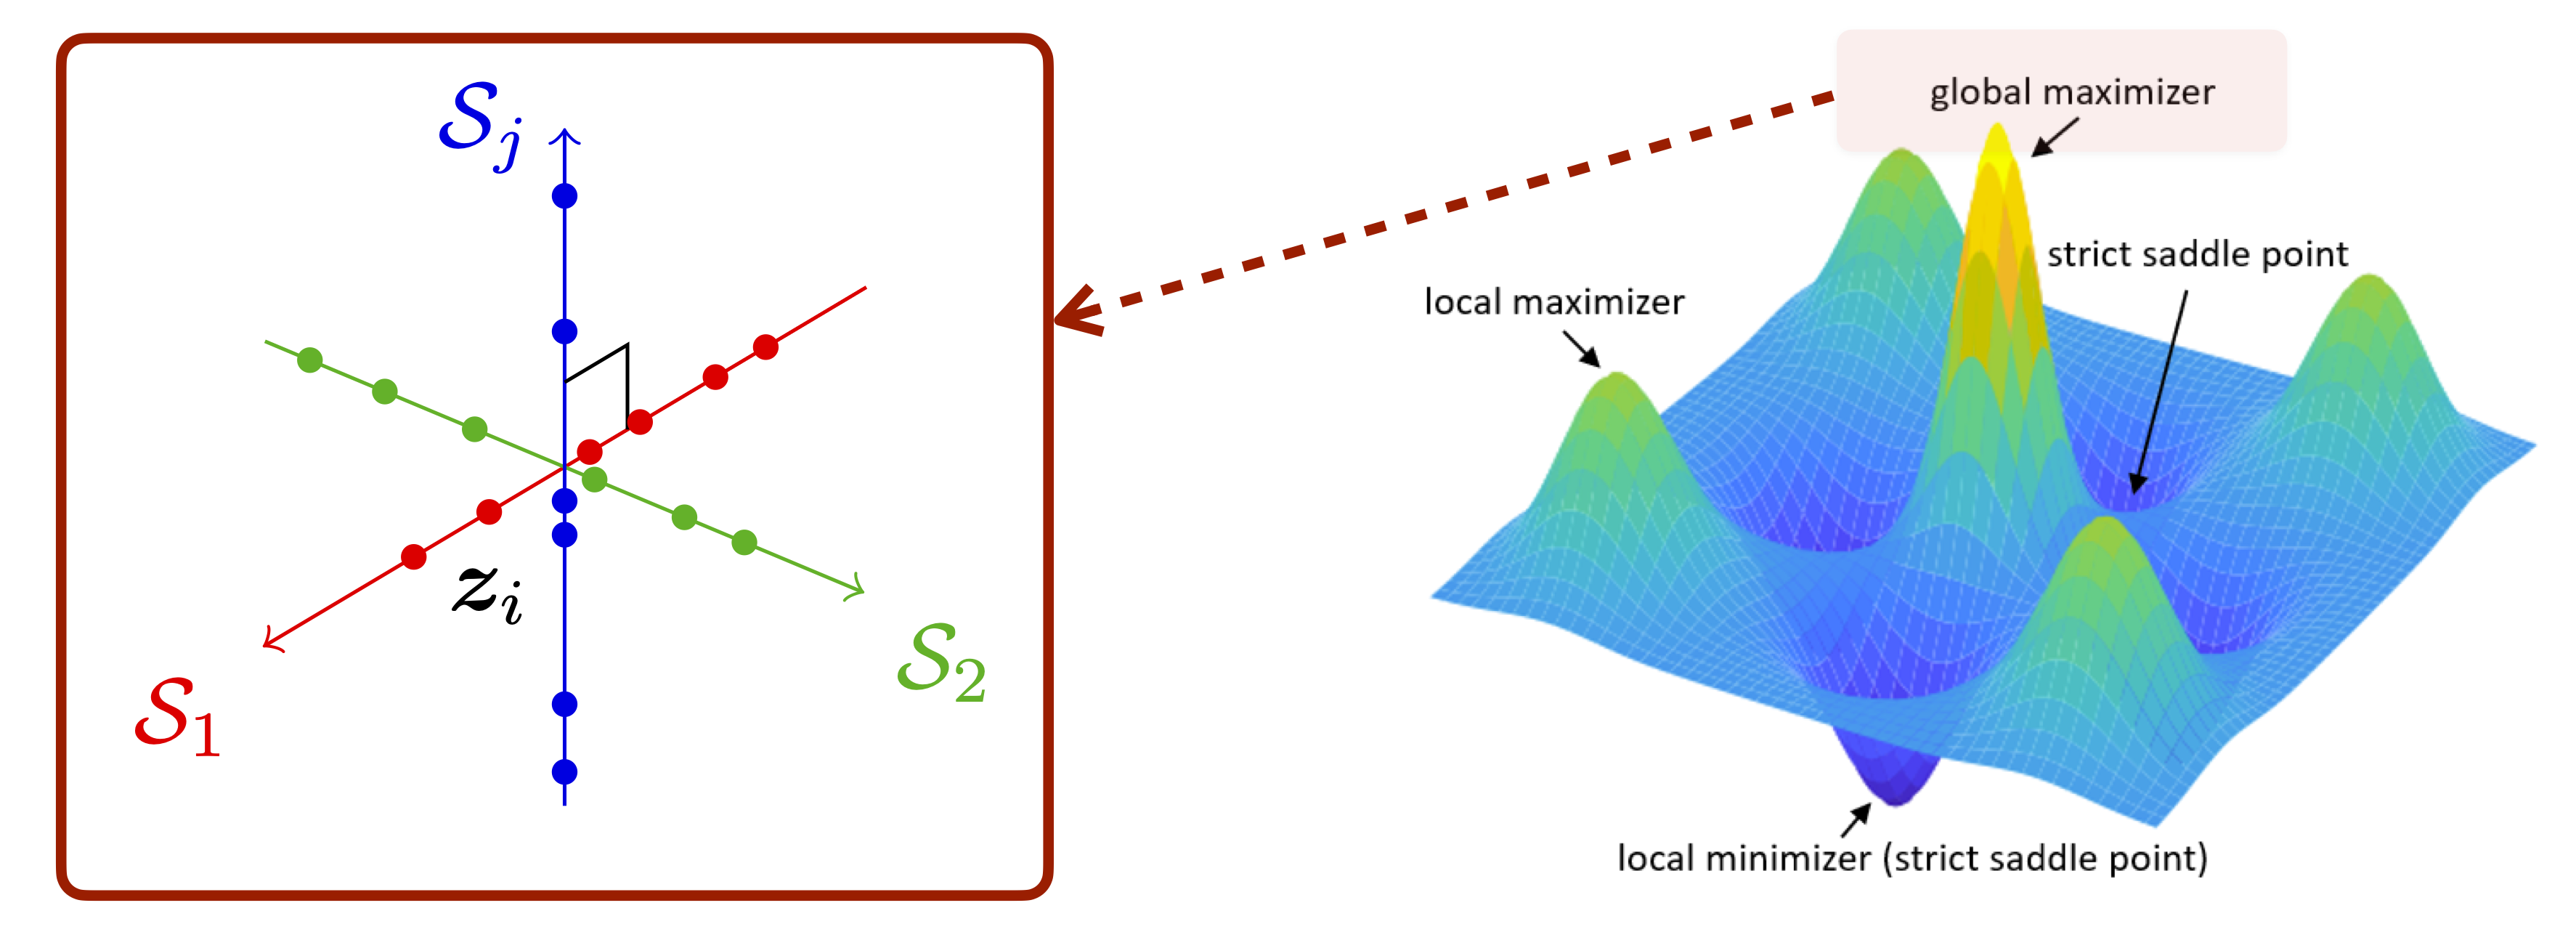
\includegraphics[width=0.8\linewidth]{\toplevelprefix/chapters/chapter3/figs/mcr2-global.png}
	\caption{{\bf Local optimization landscape:} According to Theorem \ref{thm:MCR2-properties}, the global maximum of the rate reduction objective corresponds to a solution with mutually incoherent subspaces.}
	\label{fig:mcr-global}
\end{figure}




% %\begin{wrapfigure}{r}{0.5\textwidth}
% \begin{figure}
% \begin{center}
% % \vskip -0.3in
% \includegraphics[width=0.65\textwidth]{figures_compress/pack_CompressPdf.pdf}
% \end{center}
% \vskip -0.05in
% \caption{\small Comparison of two learned representations $\Z$ and $\Z'$ via reduced rates: $R$ is the number of $\epsilon$-balls packed in the joint distribution and $R^c$ is the sum of the numbers for all the subspaces (the green balls). $\Delta R$ is their difference (the number of blue balls). The MCR$^2$ principle prefers $\Z$ (the left one).}\label{fig:sphere-packing}
% \vskip -0.15in
% \end{figure}
% %\end{wrapfigure}

% \begin{wrapfigure}{r}{0.5\textwidth}
% \vspace{-10mm}
%   \begin{center}
%     \includegraphics[width=0.47\textwidth]{figures_compress/pack_CompressPdf.pdf}%\vspace{-5mm}
%   \end{center}
%   %\addtocounter{figure}{1}
% \caption{\small Comparison of two learned representations $\Z$ and $\Z'$ via reduced rates: $R$ is the number of $\epsilon$-balls packed in the joint distribution and $R^c$ is the sum of the numbers for all the subspaces (the green balls). $\Delta R$ is their difference (the number of blue balls). The MCR$^2$ principle prefers $\Z$ (the left one).}\label{fig:sphere-packing}
% \end{wrapfigure}

\vspace{-0.1in}


\subsection{Optimization Properties of Coding Rate Reduction}
\label{sec:MCR-landscape}
% {\color{red}Geometric properties of the global optimization landscape of the rate reduction objective. MAE paper theorem that connects maximizing rate distortion to Gaussian score.}

In this subsection, we study the optimization properties of the MCR$^2$ function by analyzing its optimal solutions and the structure of its optimization landscape. To get around the technical difficulty introduced by the neural networks, we consider a simplified version of Problem \eqref{eqn:maximal-rate-reduction} as follows: 
\begin{align}\label{eqn1:maximal-rate-reduction}
    \max_{\bm Z}\ R_{\epsilon}(\Z) - R_{\epsilon}^c(\Z)\qquad \mathrm{s.t.}\quad \|\bm Z_k\|_F^2 = N_k,\ k =1,\dots,K. 
\end{align}
In theory, the MCR$^2$ principle \eqref{eqn1:maximal-rate-reduction} benefits from great generalizability and can be applied to representations $\Z$ of {\em any} distributions  as long as the rates $R_\epsilon$ and $R^c_\epsilon$ for the distributions can be accurately and efficiently evaluated. The optimal representation $\Z^{\ast}$  should have some interesting geometric and statistical properties. We here reveal nice properties of the optimal representation with the special case of subspaces, which have many important use cases in machine learning. When the desired representation for $\Z$ is multiple subspaces, the rates $R_\epsilon$ and $R^c_\epsilon$ in \eqref{eqn1:maximal-rate-reduction} are given by \eqref{chap4-eqn:coding-length-eval}
and \eqref{chap4-eqn:compress-loss-eval}, respectively. At the maximal rate reduction, MCR$^2$ achieves its optimal representations, denoted as $\Z^{\ast} = [\Z_1^*,\dots,\Z_K^*]$ with $\rank{(\Z_{k}^*)}\le d_k$. One can show that $\Z^{\ast}$ has the following desired properties (see \cite{yu2020learning} for a formal statement and detailed proofs).

\begin{theorem}[\bf Characterization of Global Optimal Solutions]
	Suppose $\Z^{\ast} = [\Z_1^*,\dots,\Z_K^*]$ is a global optimal solution of Problem~\eqref{eqn1:maximal-rate-reduction}. The following statements hold: 
	\begin{itemize}
		\item {\em Between-Class Discriminative}: As long as the ambient space is adequately large ($d \ge \sum_{k=1}^{K} d_k$), the subspaces are all orthogonal to each other, {\em i.e.}, $(\Z_{k}^*)^{\top} \Z_{l}^* = \bm{0}$ for $k \not= l$.
		\item {\em Maximally Diverse Representation}:
		      As long as the coding precision is adequately high, i.e., $\epsilon ^4 < c\cdot \min_{k}\left\{ \frac{N_k}{N}\frac{d^2}{d_k^2}\right\}$, where $c>0$ is a constant. Each subspace achieves its maximal dimension, i.e. $\mathrm{rank}{(\Z_{k}^*)}= d_k$. In addition, the largest $d_k-1$ singular values of $\Z_{k}^*$ are equal.
		      \label{thm:MCR2-properties}
	\end{itemize}
	% \vspace{-2mm}
\end{theorem}

% \begin{figure}[t]
% % \vspace{-5mm}
%     % 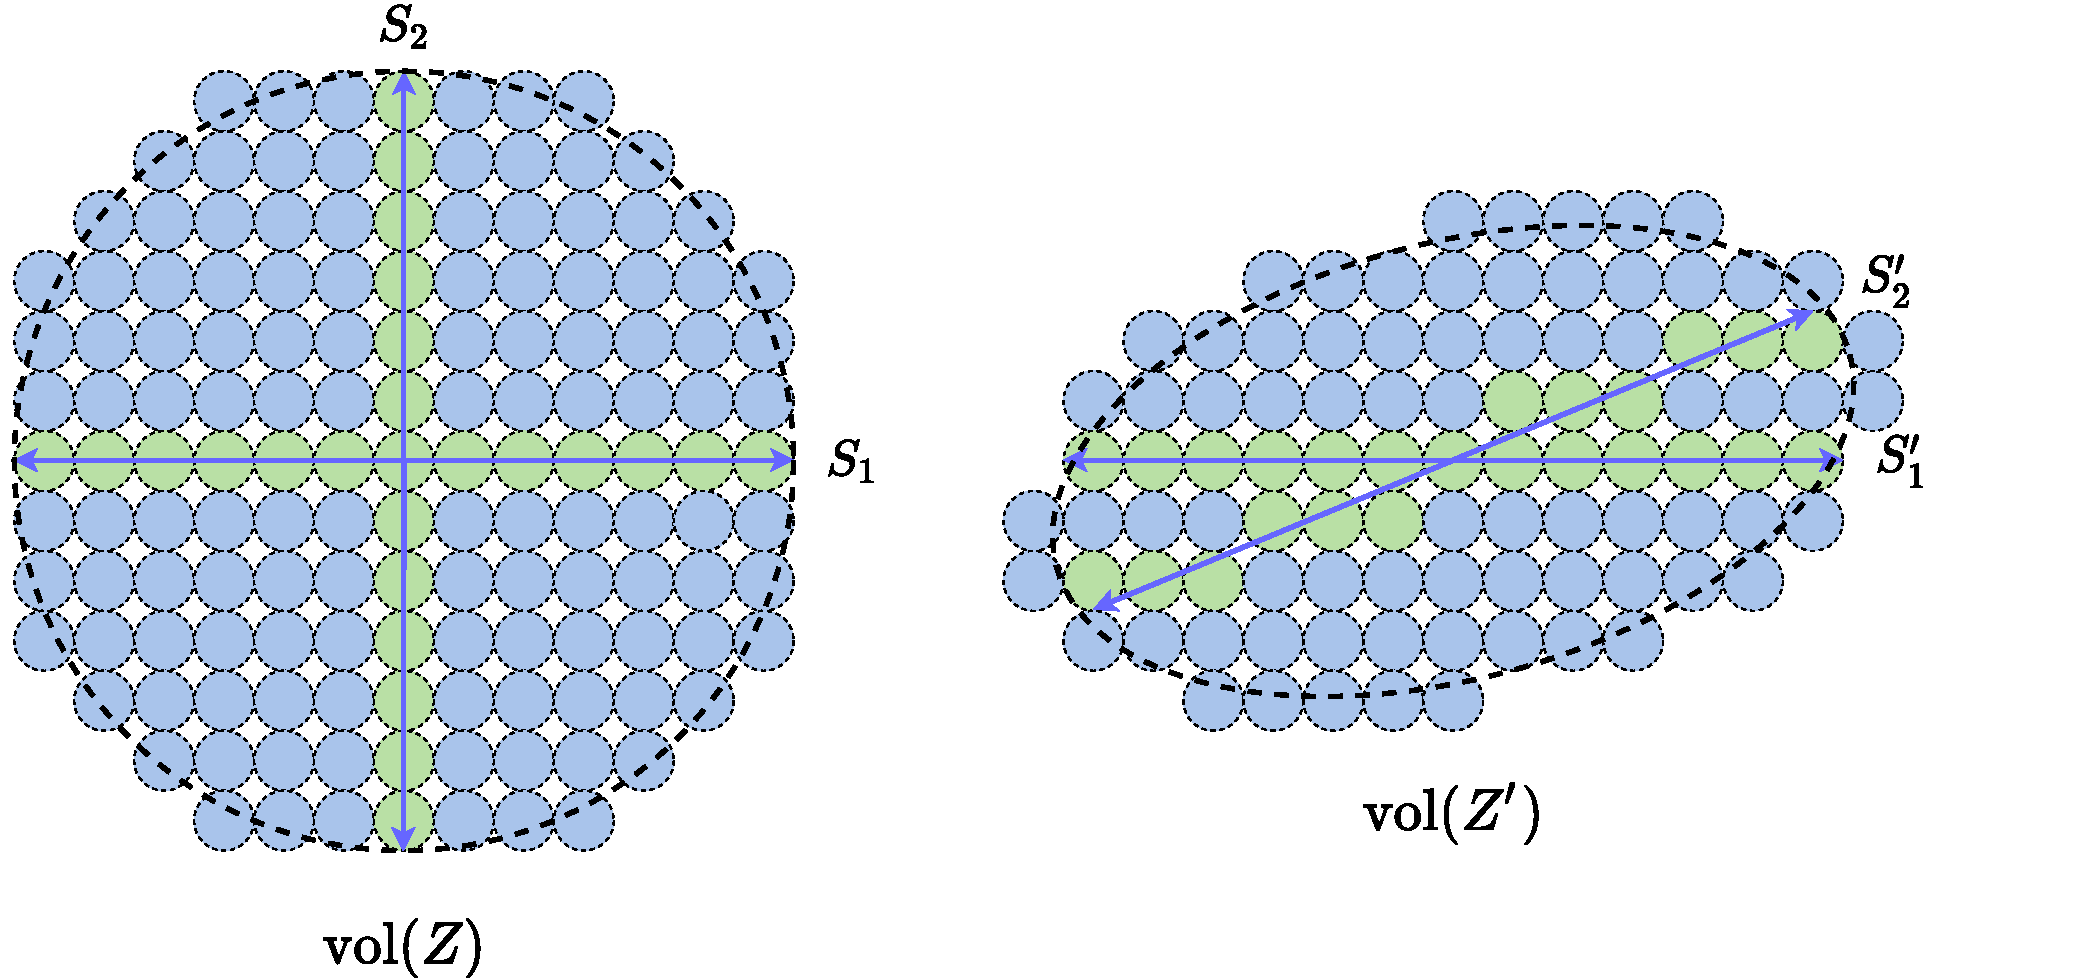
\includegraphics[width=0.7\textwidth]{chapters/chapter3/figs/pack_Compress.pdf}
% % \vspace{-15mm}
% \caption{\small Comparison of two learned representations $\Z$ and $\Z'$ via reduced rates: $R$ is the number of $\epsilon$-balls packed in the joint distribution and $R^c$ is the sum of the numbers for all the subspaces (the green balls). $\Delta R$ is their difference (the number of blue balls). The MCR$^2$ principle prefers $\Z$ (the left one).}\label{fig:sphere-packing}
% \vspace{-3mm}
% \end{figure}

This theorem indicates that the MCR$^2$ principle promotes embedding of data into multiple independent subspaces (as illustrated in Figure \ref{fig:mcr-global}), with features distributed {\em isotropically}  in each subspace (except for possibly one dimension). Notably, this theorem also confirms that the features learned by the MCR$^2$ principle exhibit the desired low-dimensional discriminative properties discussed in \Cref{subsec:LDR}. In addition, among all such discriminative representations, it prefers the one with the highest dimensions in the ambient space. This is substantially different from the objective of information bottleneck~\eqref{chap4-eqn:information-bottleneck}.
% \pw{add some transition here to connect MCR$^2$ to the regularized MCR$^2$}\yaodong{TODO: motivation: an equivalent formulation allows more fine-grained optimization landscape analysis?}



\begin{example}[Classification of Images on CIFAR-10]
	We here present how the MCR$^2$ objective helps learn better representations than the cross entropy \eqref{chap4-eqn:cross-entropy} for image classification. Here we adopt the popular neural network architecture, the ResNet-18~\cite{he2016deep}, to model the feature mapping $\z = f(\x,\theta)$. We optimize the neural network parameters $\theta$ to maximize the coding rate reduction. We evaluate the performance with the CIFAR10 image classification dataset~\cite{krizhevsky2009learning}.

	\begin{figure}[t]
		\begin{subfigure}[t]{0.42\textwidth}
			\centering
			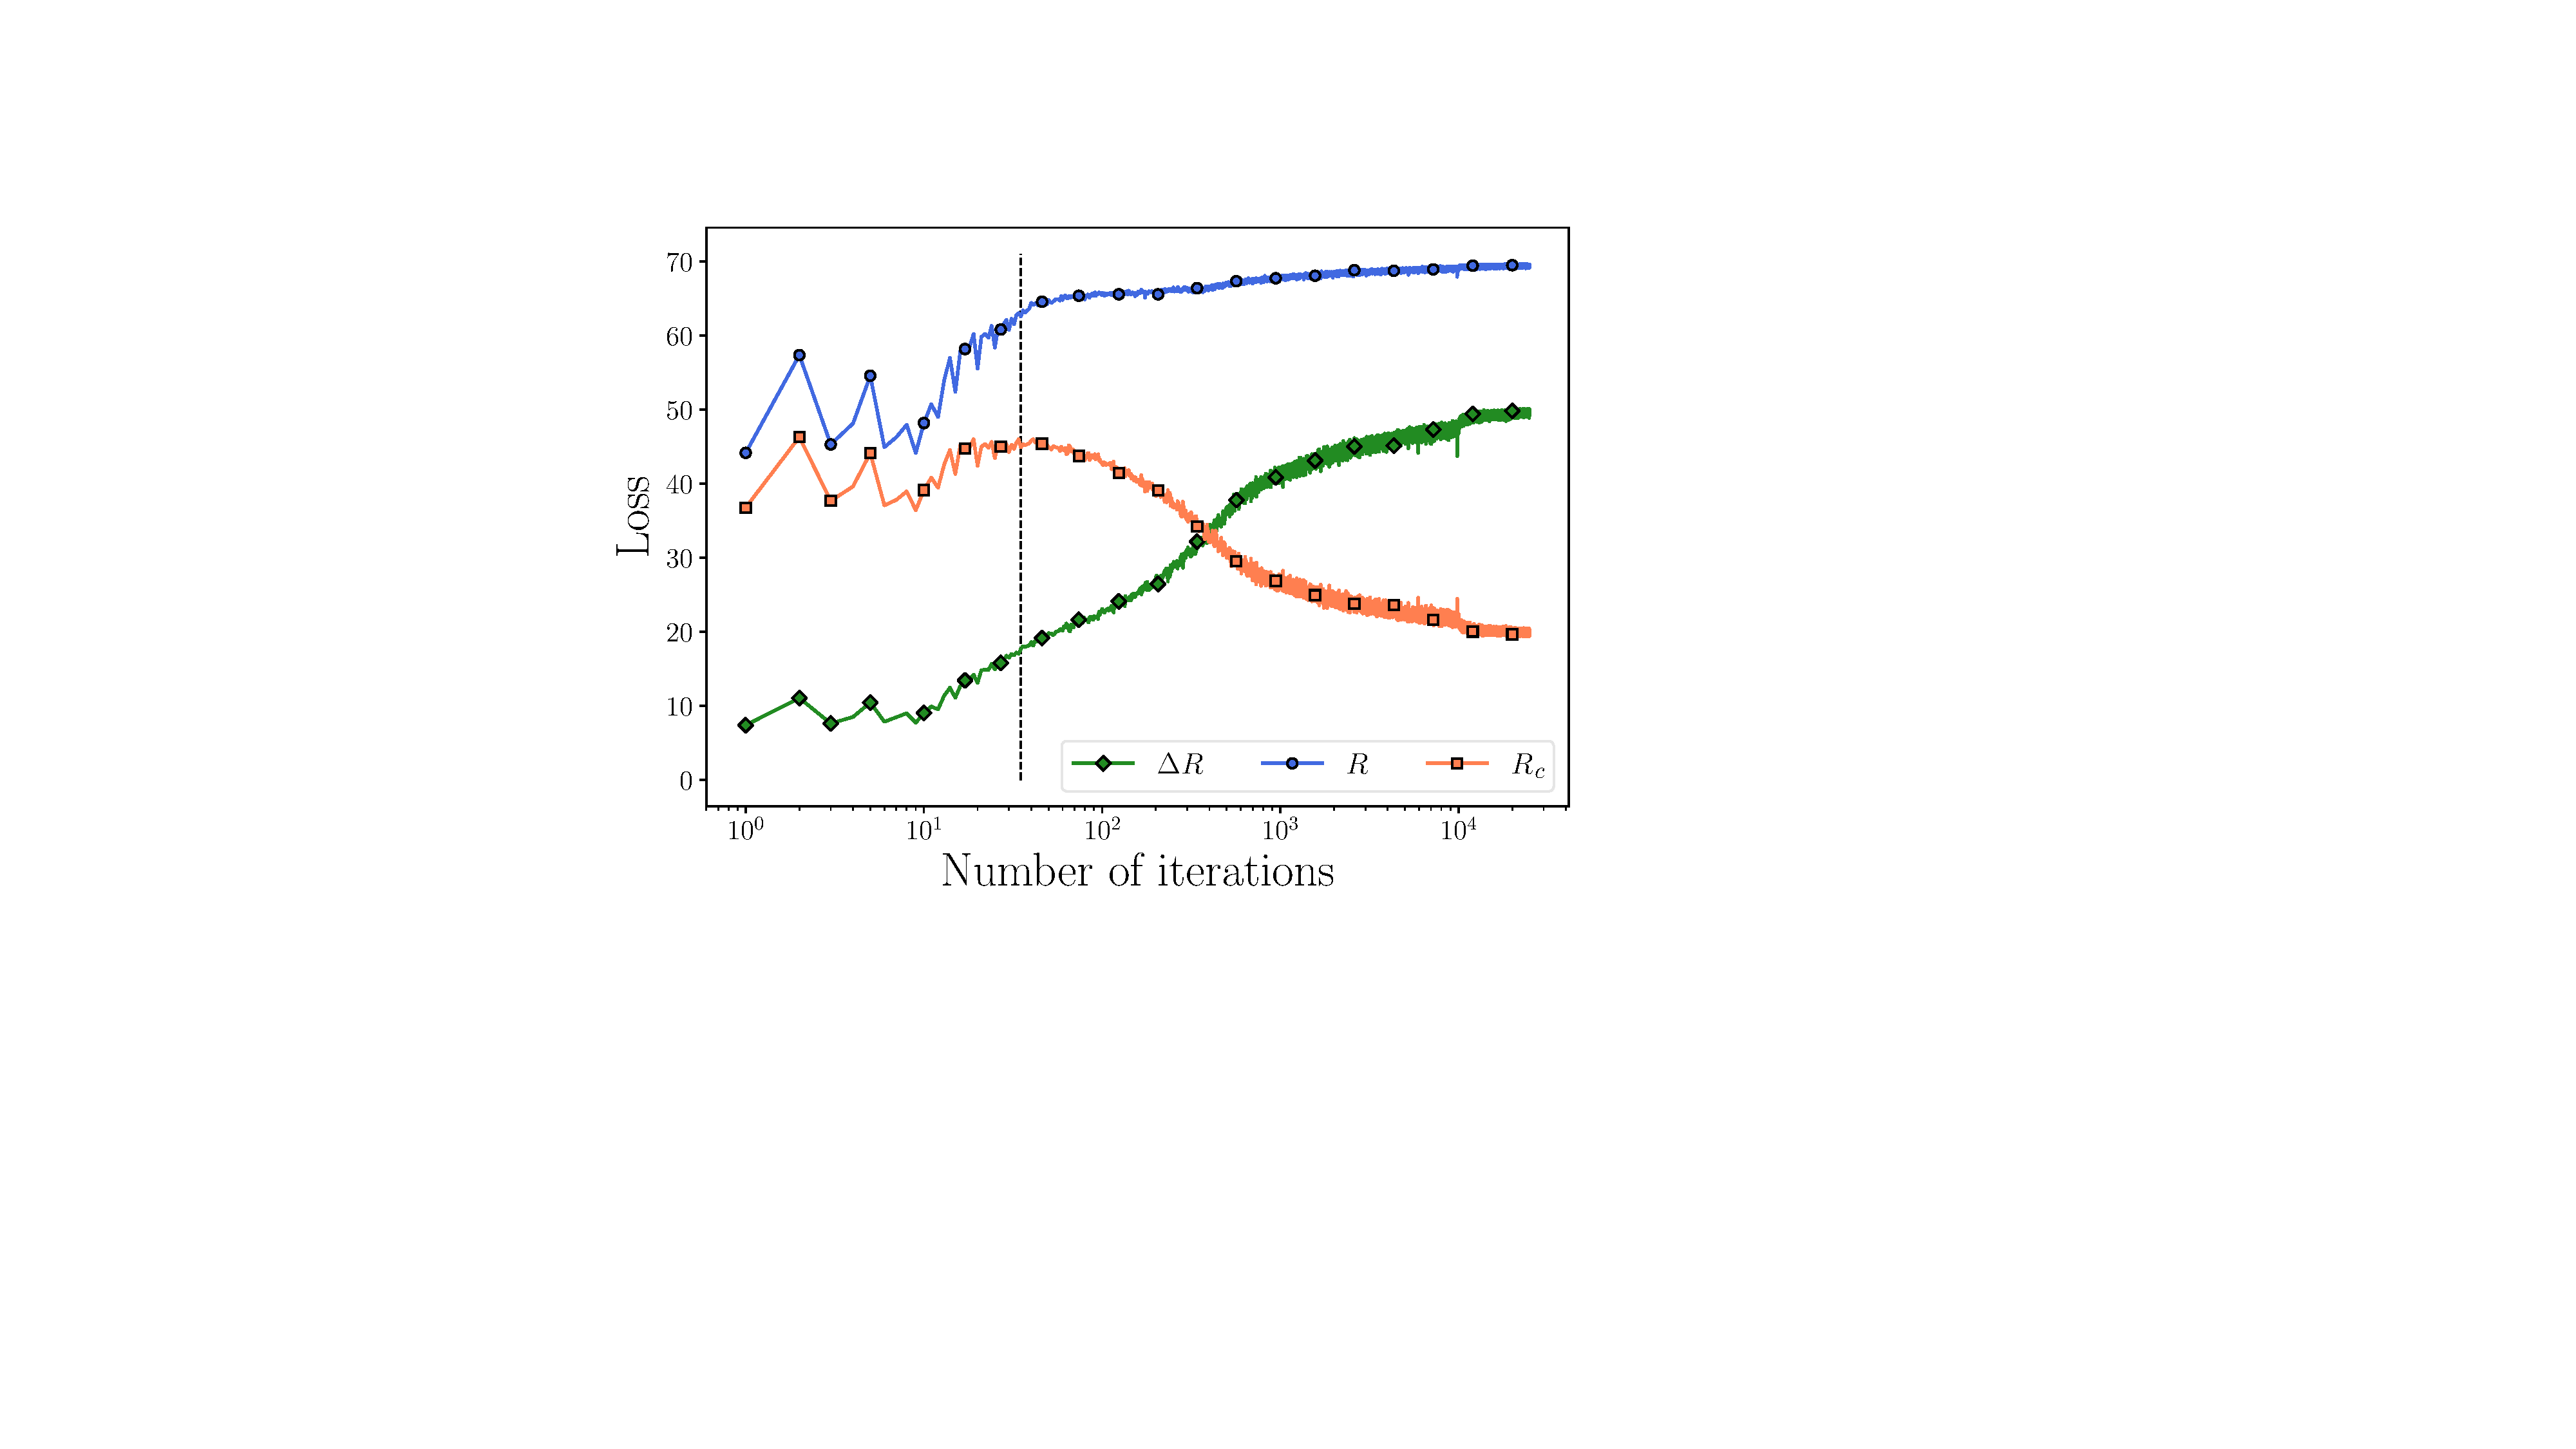
\includegraphics[width=\textwidth]{\toplevelprefix/chapters/chapter3/figs/loss_log.pdf}
			\caption{Evolution of $R_\epsilon$, $R^c_\epsilon$, $\Delta R_\epsilon$ during the training process.}
			\label{fig:train-test-loss-pca-1}
		\end{subfigure}
		\hfill
		\begin{subfigure}[t]{0.42\textwidth}
			\centering
			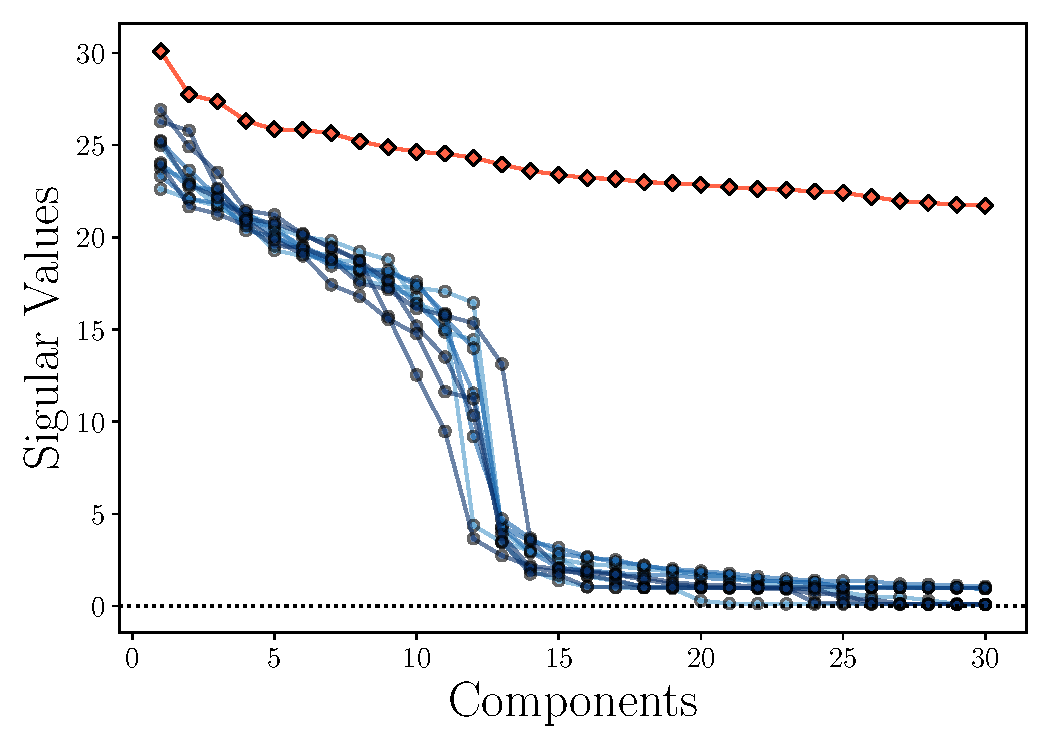
\includegraphics[width=\textwidth]{\toplevelprefix/chapters/chapter3/figs/pca_mainline.pdf}
			\caption{PCA: {\small (\textbf{red}) overall data; (\textbf{blue}) individual classes}.}
			\label{fig:train-test-loss-pca-3}
		\end{subfigure}
		\caption{\small Evolution of the rates of MCR$^2$ in the training process, the principal components of learned features.}
		\label{fig:train-test-loss-pca}
	\end{figure}

	% \begin{figure}[t]
	%     %\includegraphics[width=0.47\textwidth]{chapters/chapter3/figs/heatmap_mcr2.pdf}
	%     %\includegraphics[width=0.47\textwidth]{figs_chap4/heatmap_ce.pdf}
	%     \caption{\small Cosine similarity between  learned features by using the MCR$^2$ objective  (\textbf{left}) and CE loss (\textbf{right}).}
	%     \label{fig:heatmap-plot}
	% \end{figure}

	\begin{figure*}[b]
		\begin{center}

			\includegraphics[width=0.42\textwidth]{\toplevelprefix/chapters/chapter3/figs/heatmap_mcr2.pdf}
			\hspace{0.25cm}
			\includegraphics[width=0.42\textwidth]{\toplevelprefix/chapters/chapter3/figs/heatmap_ce.png}
			\caption{\small Cosine similarity between learned features by using the MCR$^2$ objective  (\textbf{left}) and CE loss (\textbf{right}).}
			\label{fig:heatmap-plot}
		\end{center}
		\vskip -0.1in
	\end{figure*}

	Figure~\ref{fig:train-test-loss-pca-1} illustrates how the two rates and their difference (for both training and test data) evolves over epochs of training: After an initial phase, $R_\epsilon$ gradually increases while $R^c_\epsilon$ decreases, indicating that features $\bm Z$ are expanding as a whole while each class $\bm Z_k$ is being compressed.
	Figure~\ref{fig:train-test-loss-pca-3} shows the distribution of singular values per $\Z_k$.  Figure~\ref{fig:heatmap-plot} shows the cosine similarities between the learned features sorted by class. We compare the similarities of the learned features by using the cross-entropy \eqref{chap4-eqn:cross-entropy} and the MCR$^2$ objective \eqref{eqn:maximal-rate-reduction}. From the plots, one can clearly see that the representations learned by using MCR$^2$ loss are much more diverse than the ones learned by using cross-entropy loss. More details of this experiment can be found in \cite{chan2021redunet}.
	%In addition, we find that we are able to select diverse images from the same class according to the ``principal'' components of the learned features (see Figure~\ref{fig:visual-class-2-8} and Figure~\ref{fig:visual-overall-data}).
	\label{eg:Rate-Reduction-CIFAR10}
\end{example}

%\yima{I would suggest the above example is better moved to the Chapter 3. To justify the rate reduction objective function and its landscape.}

However, there has been an apparent lack of justification of the network architectures used in the above experiments. It is yet unclear why the network adopted here (the ResNet-18) is suitable for representing the map $f(\x, \theta)$, let alone for interpreting the layer operators and parameters $\theta$ learned inside. In the next chapter, {\em we will show how to derive network architectures and components entirely as a ``white box'' from the desired objective (say the rate reduction)}.



\paragraph{Regularized MCR$^2$.}
The above theorem characterizes properties of the global optima of the rate reduction objectives. What about other optima, such as local ones?  Due to the constraints of the Frobenius norm, it is a difficult task to analyze Problem \eqref{eqn1:maximal-rate-reduction} from an optimization-theoretic perspective. Therefore, we consider the Lagrangian formulation of \eqref{eqn1:maximal-rate-reduction}. This can be viewed as a tight relaxation or even an equivalent problem of \eqref{eqn1:maximal-rate-reduction} whose optimal solutions agree under specific settings of the regularization parameter; see \cite[Proposition 1]{wang2024global}.
Specifically, the formulation we study, referred to henceforth as the \textit{regularized MCR$^2$ problem}, is as follows:
\begin{align}\label{eq:MCR-reg}
	\max_{\bm Z}\ R_{\epsilon}(\Z) - R_{\epsilon}^c(\Z) - \frac{\lambda}{2}\|\bm Z\|_F^2,
\end{align}
where $\lambda > 0$ is the regularization parameter. Although the program  \eqref{eq:MCR-reg} is highly nonconcave and involves matrix inverses in its gradient computation, we can still explicitly characterize its local and global optima as follows.

\begin{theorem}[\bf Local and Global Optima]\label{thm:mcr-global-opt}
	Let $N_k$ denote the number of training samples in the $k$-th class for each $k \in \{1,\dots,K\}$, $N_{\max} \doteq \max\{N_1,\dots,N_K\}$, $\alpha=d/(N\epsilon^2)$, and $\alpha_{k} = d/(N_k\epsilon^2)$ for each $k \in \{1,\dots,K\}$. Given a coding precision $\epsilon > 0$, if the regularization parameter satisfies
	\begin{align}\label{eq:lambda}
		\lambda \in \left(0, \frac{d(\sqrt{N/N_{\max}}-1)}{N(\sqrt{N/N_{\max}}+1)\epsilon^2} \right],
	\end{align}
	then the following statements hold: \\
	(i) ({\bf Local maximizers}) $\bm Z^* = \left[\bm Z_1^*,\dots,\bm Z_K^* \right]$ is a local maximizer of Problem \eqref{eq:MCR-reg} if and only if the $k$-th block admits the following decomposition
	\begin{align}\label{eq:Zk opti}
		\bm Z_k^* = \left(\frac{ \eta_k + \sqrt{\eta_k^2 - 4\lambda^2N/N_k}}{2\lambda \alpha_{k}}\right)^{1/2} \bm U_k \bm V_k^\top,
	\end{align}
	where (a) $r_k = \mathrm{rank}(\bm Z_k^*)$ satisfies $r_k \in [0,\min\{N_k,d\})$ and $\sum_{k=1}^K r_k \le \min\{N,d\}$, (b) $\bm U_k \in \mathcal{O}^{d \times r_k}$ satisfies $\bm U_k^{\top}\bm U_l = \bm 0$ for all $k \neq l$, $\bm V_k \in \mathcal{O}^{N_k \times r_k}$, and (c) $\eta_k=(\alpha_k-\alpha) - \lambda(N/N_k+1)$ for each $k\in \{1,\dots,K\}$.
	\\
	(ii) ({\bf Global maximizers}) $\bm Z^* = \left[\bm Z_1^*,\dots,\bm Z_K^* \right]$ is a global maximizer of Problem \eqref{eq:MCR-reg} if and only if (a) it satisfies the above all conditions and $\sum_{k=1}^K r_k = \min\{m,d\}$, and (b) for all $k \neq l \in [K]$ satisfying $N_k < N_l$ and $r_l > 0$, we have $r_k = \min\{N_k,d\}$.
\end{theorem}

\begin{figure}[t]
	\centering
	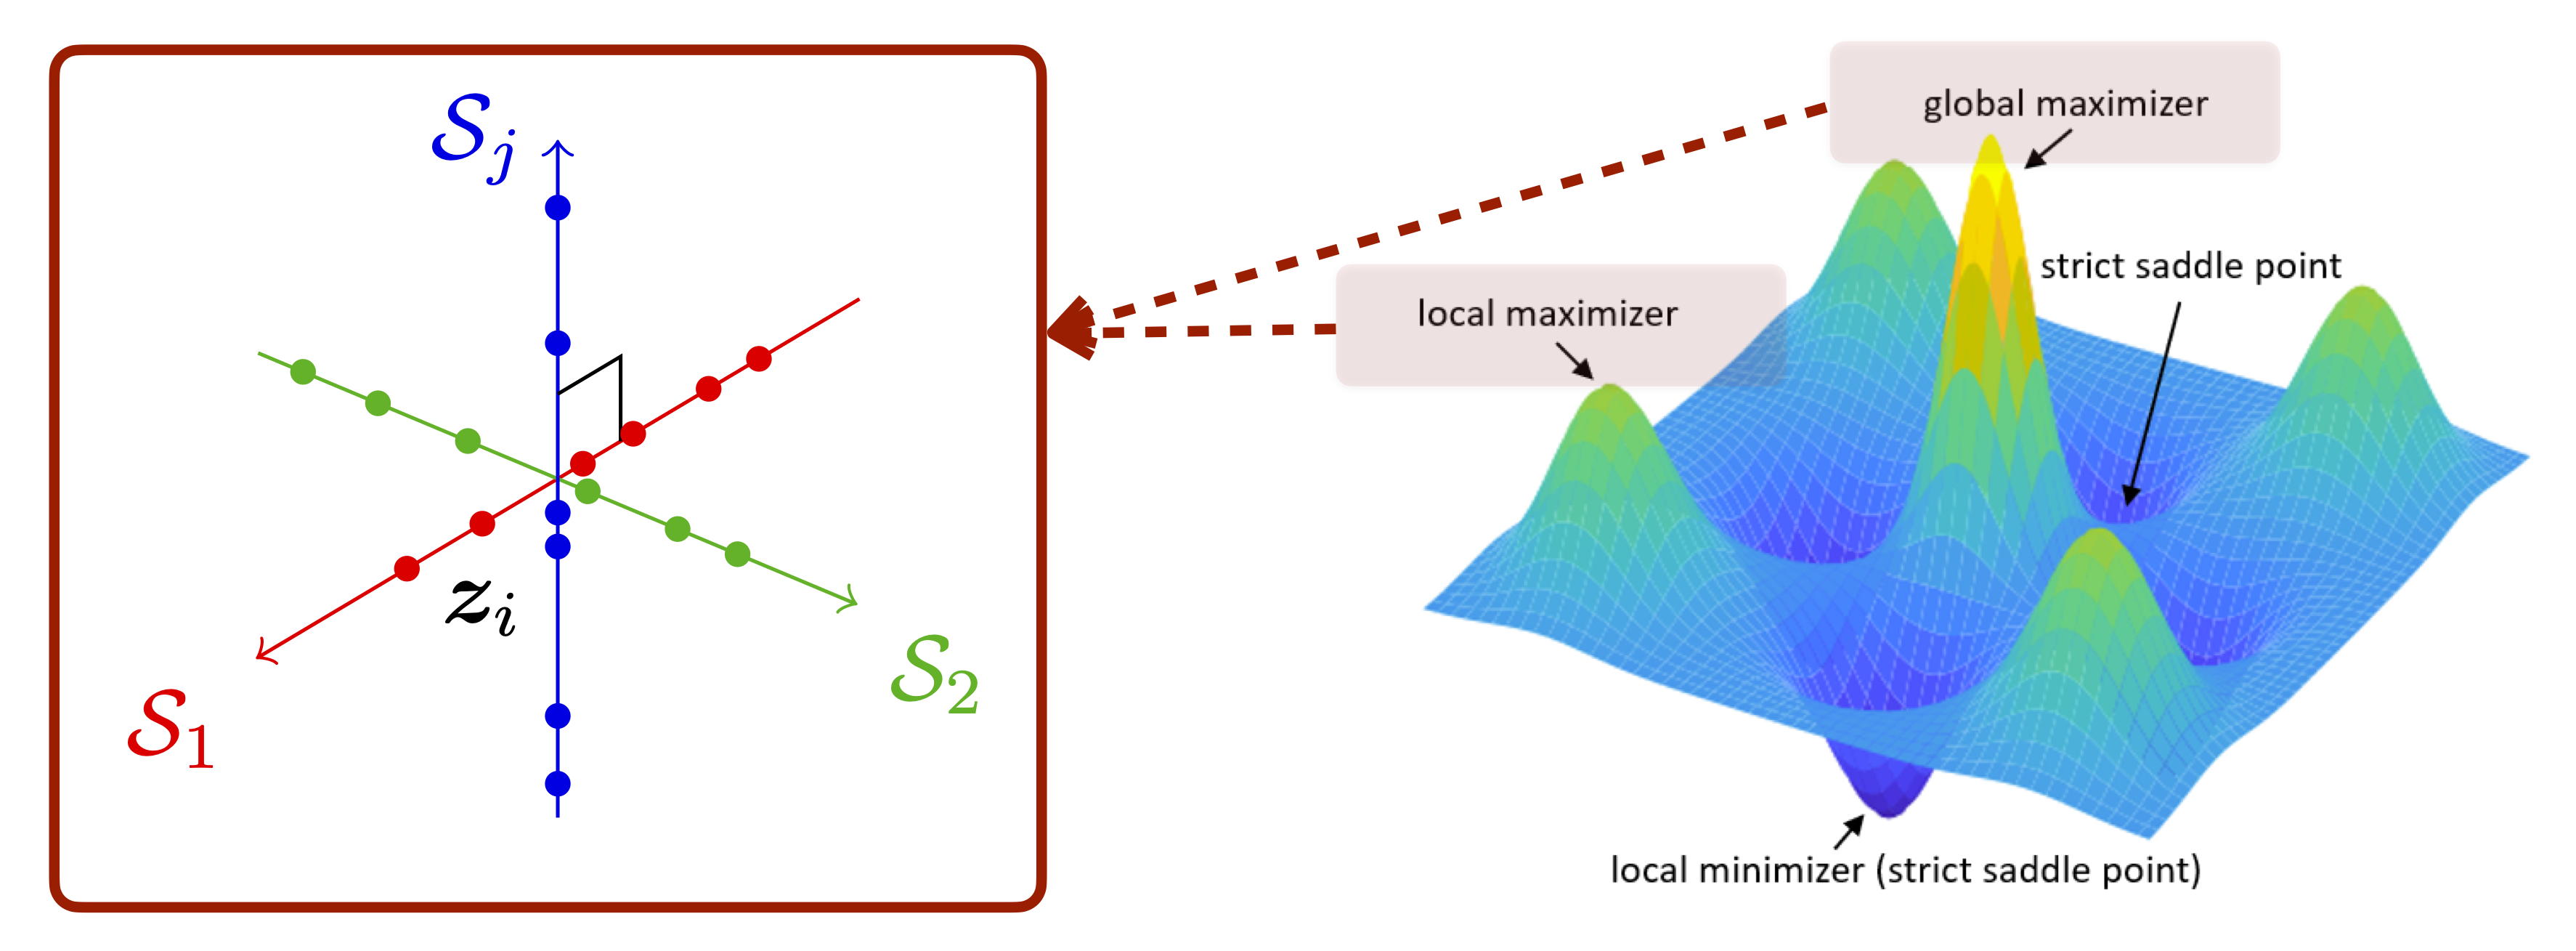
\includegraphics[width=0.8\linewidth]{\toplevelprefix/chapters/chapter3/figs/mcr2-global-local.png}
	\caption{{\bf Global optimization landscape:} According to \cite{sun2015nonconvex,lee2016gradient}, \Cref{thm:mcr-global-opt,thm:mcr-benign-opt-landscape}, both global and local maxima of the (regularized) rate reduction objective correspond to a solution with mutually incoherent subspaces. All other critical points are strict saddle points.}
	\label{fig:mcr-global-local}
\end{figure}

This theorem explicitly characterizes the local and global optima of problem \eqref{eq:MCR-reg}. Intuitively, this shows that the features represented by each local maximizer of Problem \eqref{eq:MCR-reg} are low-dimensional and discriminative. Although we have characterized the local and global optimal solutions in Theorem~\ref{thm:mcr-global-opt}, it remains unknown whether these solutions can be efficiently computed using GD to solve the problem \eqref{eq:MCR-reg}, since GD may get stuck at other critical points such as a saddle point.
Fortunately, \cite{sun2015nonconvex,lee2016gradient} showed that if a function is twice continuously differentiable and satisfies the {\em strict saddle property}, i.e., each critical point is either a local minimizer or a strict saddle point\footnote{We say that a critical point is a strict saddle point of Problem \eqref{eq:MCR-reg} if it has a direction with strictly positive curvature~\cite{sun2015nonconvex}. This includes classical saddle points with strictly positive curvature as well as local minimizers.}, GD converges to its local minimizer almost surely with random initialization. We investigate the global optimization landscape of the problem \eqref{eq:MCR-reg} by characterizing all its critical points as follows.

 \begin{theorem}[\bf Benign Global Optimization Landscape]\label{thm:mcr-benign-opt-landscape}
	Given a coding precision $\epsilon > 0$, if the regularization parameter satisfies \eqref{eq:lambda},
	it holds that any critical point $\bm Z$ of the problem \eqref{eq:MCR-reg} is either a local maximizer or a strict saddle point.
\end{theorem}
Together, the above two theorems
show that the learned features associated with each local maximizer of the rate
reduction objective---not just global maximizers---are structured as incoherent low-dimensional subspaces. Furthermore, the (regularized) rate reduction objective \eqref{eqn:maximal-rate-reduction} has a very benign landscape with only local maxima and strict saddles as critical points, as illustrated in Figure \ref{fig:mcr-global-local}. 
% To our knowledge, \Cref{thm:mcr-global-opt,thm:mcr-benign-opt-landscape} constitute the first analysis of local optima and optimization landscapes for MCR$^2$ objectives. 
According to \cite{sun2015nonconvex,lee2016gradient}, \Cref{thm:mcr-global-opt,thm:mcr-benign-opt-landscape} imply that low-dimensional and discriminative representations (LDRs) can be efficiently found by applying (stochastic) gradient descent to the rate reduction objective \eqref{eqn:maximal-rate-reduction} from random initialization. These results also indirectly explain why in Example \ref{eg:Rate-Reduction-CIFAR10}, if the chosen network is expressive enough and trained well, the resulting representation typically gives an incoherent linear representation which likely corresponds to the globally optimal solution.
Interested readers are referred to \cite{wang2024global} for proofs. 



%\subsection{Classification via minimal incremental coding length}
%\href{http://people.eecs.berkeley.edu/~yima/psfile/MICL_SJIS.pdf}{supervised classification} from the perspective of (lossy) compression.

\section{Summary and Notes}

The use of denoising and diffusion for sampling has a rich history. The first work which is clearly about a diffusion model is probably \cite{Sohl-Dickstein2015}, but before this there are many works about denoising as a computational and statistical problem. The most relevant of these is probably \cite{hyvarinen05a}, which explicitly uses the score function to denoise (as well as perform independent component analysis). The most popular follow-ups are basically co-occurring: \cite{ho2020denoising,song2019}. Since then, thousands of papers have built on diffusion models; we will revisit this topic in \Cref{ch:autoencoding}.

Many of these works use a different stochastic process than the simple linear combination \eqref{eq:gen_additive_gaussian_noise_model}. In fact, all works listed above emphasize the need to add \textit{independent} Gaussian noise at the beginning of each step of the forward process. Theoretically-minded work actually uses Brownian motion or stochastic differential equations to formulate the forward process \cite{song2020score}. However, since linear combinations of Gaussians still result in Gaussians, the \textit{marginal distributions} of such processes still take the form of \eqref{eq:gen_additive_gaussian_noise_model}. Most of our discussion requires only that the marginal distributions are what they are, and hence our overly simplistic model is actually quite enough for almost everything. In fact, the only time where marginal distributions are not enough is when we derive an expression for \(\Ex[\vx_{s} \mid \vx_{t}]\) in terms of \(\Ex[\vx \mid \vx_{t}]\). Different (noising) processes give different such expressions, which can be used for sampling (and of course there are other ways to derive efficient samplers, such as the ever-popular DDPM sampler). The process in \eqref{eq:gen_additive_gaussian_noise_model} is a bona fide stochastic process, however, whose ``natural'' denoising iteration takes the form of the popular DDIM algorithm \cite{song2020denoising}. (Even this equivalence is not trivial; we cite \cite{de2025distributional} as a justification.) 

% {Lossy coding does more than just quantization. It allows us to avoid a pathological solution by simply using the empirical distribution as the optimal solution that minimizes entropy. }

% {From the achievable (entropy) to an implementable coding scheme. That is, in addition to a computable or achievable encoding scheme, there should also exist an implementable decoding scheme. Lossy quantization becomes necessary for real-valued data.} 

On top of the theoretical work \citep{li2024d} covered in \Cref{sec:denoising-intro}, and the lineage of work that it builds on, which studies the \textit{sampling} efficiency of diffusion models when the data has low-dimensional structure, there is a large body of work which studies the \textit{training} efficiency of diffusion models when the data has low-dimensional structure. Specifically, \citet{chen2023score} and \citep{wang2024diffusion} characterized the approximation and estimation error of denoisers when the data belongs to a mixture of low-rank Gaussians, showing that the number of training samples required to accurately learn the distribution scales with the intrinsic dimension of the data rather than the ambient distribution. There is considerable \textit{methodological} work which attempts to utilize the low-dimensional structure of the data in order to do various things with diffusion models. We highlight three here: image editing \citep{chen2024exploring}, watermarking \citep{li2024shallow}, and unlearning \citep{chen2025dual}, though as always this is an inexhaustive list.
 
% On top of the work \citep{li2024adapting} covered in \Cref{sec:denoising-intro}, many studies have drawn increasing attention to the training and sampling efficiency of diffusion models when the image data has low-dimensional structures. On the training side, \cite{chen2023score} provided a theoretical framework for understanding how diffusion models perform when the data lie on or near low-dimensional manifolds. It rigorously analyzes the approximation and estimation errors of score functions under manifold settings and demonstrates that diffusion models can achieve efficient distribution recovery with sample and computational complexities that depend on the intrinsic, rather than ambient, dimensionality of the data. Later, \cite{wang2024diffusion} extended the analysis and provided compelling theoretical and empirical evidence that diffusion models can be trained efficiently when the data distribution lies near a union of low-dimensional subspaces. Specifically, they show that the number of training samples required to accurately learn a mixture of low-rank Gaussian distributions scales linearly with the intrinsic dimension of the data. These works indicate that diffusion models are capable of leveraging low-dimensional structures inherent in image data, leading to significant improvements in training efficiency. On the sampling side, \cite{li2024adapting} showed that when the underlying distribution lies on or near a low-dimensional manifold in the high-dimensional space, denosing diffusion probabilistic model (DDPM) sampler can adapt to low-dimensional structures and achieves a sampling rate at the order of $O(k^2/\sqrt{T})$, where $k$ is the instinct dimension and $T$ is the number of steps. Recently, \cite{liang2025low} analyzed how diffusion generative models leverage unknown low-dimensional structures to accelerate sampling. They showed that the DDPM sample achieves a sampling rate at the order of $O(k/T)$. \cite{tang2024adaptivity} showed that both Langevin diffusion and forward-backward diffusion models can adapt to the intrinsic manifold structure and the sampling rate of the inducing distribution estimator depends only on the intrinsic dimension of the data. These results collectively demonstrate that diffusion models can effectively exploit intrinsic low-dimensional structures in the data to significantly improve sampling efficiency. 











% \pw{Add some references on computational and sampling efficiency of diffusion models and discuss these results.}




\section{Exercises and Extensions}

\begin{exercise}
    Please show that \eqref{eq:optimal_denoiser} is the optimal solution of Problem \eqref{eq:denoising_loss}. 
\end{exercise}

\begin{exercise}\label{exercise:conditional_gaussian}
  Consider random vectors $\vx \in \bR^D$ and $\vy \in \bR^d$, such that the
  pair $(\vx, \vy) \in \bR^{D + d}$ is jointly Gaussian. This means that
  \begin{equation*}
    \begin{bmatrix}
      \vx \\
      \vy
    \end{bmatrix}
    \sim
    \cN \left(
      \begin{bmatrix}
        \vmu_{\vx} \\
        \vmu_{\vy}
      \end{bmatrix}
      ,
      \begin{bmatrix}
        \vSigma_{\vx} & \vSigma_{\vx\vy} \\
        \vSigma_{\vx\vy}^\top & \vSigma_{\vy}
      \end{bmatrix}
    \right),
  \end{equation*}
  where the mean and covariance parameters are given by
  \begin{equation*}
    \vmu_{\vx} = \bE[\vx],\quad \vmu_{\vy} = \bE[\vy],\quad
    \begin{bmatrix}
      \vSigma_{\vx} & \vSigma_{\vx\vy} \\
      \vSigma_{\vx\vy}^\top & \vSigma_{\vy}
    \end{bmatrix}
    =
    \bE\left[
      \begin{bmatrix}
        \vx - \bE[\vx] \\
        \vy - \bE[\vy]
      \end{bmatrix}
      \begin{bmatrix}
        \vx - \bE[\vx] \\
        \vy - \bE[\vy]
      \end{bmatrix}^\top
      \right]
  \end{equation*}
  Assume that $\vSigma_{\vy}$ is positive definite (hence invertible); then
  positive semidefiniteness of the covariance matrix is equivalent to the Schur
  complement condition $\vSigma_{\vx} - \vSigma_{\vx\vy} \vSigma_{\vy}^{-1}
  \vSigma_{\vx\vy}^\top \succeq \Zero$.

  In this exercise, we will prove that the conditional distribution $p_{\vx \mid
  \vy}$ is Gaussian: namely,
  \begin{equation}\label{eq:gaussian-conditional-eqn}
    p_{\vx \mid \vy} \sim \cN\left(
      \vmu_{\vx} + \vSigma_{\vx\vy} \vSigma_{\vy}^{-1} (\vy - \vmu_{\vy}),
      \vSigma_{\vx} - \vSigma_{\vx\vy} \vSigma_{\vy}^{-1}
      \vSigma_{\vx\vy}^{\top}
    \right).
  \end{equation}
  A direct path to prove this result manipulates the defining ratio of
  densities $p_{\vx, \vy} / p_{\vy}$. We sketch an algebraically-concise
  argument of this form below.

  \begin{enumerate}
    \item Verify the following matrix identity for the covariance:
      \begin{equation}\label{eq:gaussian-conditional-covariance-block}
        \begin{bmatrix}
          \vSigma_{\vx} & \vSigma_{\vx\vy} \\
          \vSigma_{\vx\vy}^\top & \vSigma_{\vy}
        \end{bmatrix}
        =
        \begin{bmatrix}
          \vI_D & \vSigma_{\vx\vy}\vSigma_{\vy}^{-1} \\
          \Zero & \vI_d
        \end{bmatrix}
        \begin{bmatrix}
          \vSigma_{\vx} - \vSigma_{\vx\vy} \vSigma_{\vy}^{-1}
          \vSigma_{\vx\vy}^{\top} & \Zero \\
          \Zero & \vSigma_{\vy}
        \end{bmatrix}
        \begin{bmatrix}
          \vI_D & \Zero\\
          \vSigma_{\vy}^{-1}\vSigma_{\vx\vy}^\top & \vI_d
        \end{bmatrix}.
      \end{equation}
      One arrives at this identity by performing two rounds of (block) Gaussian
      elimination on the covariance matrix.
    \item Based on the previous identity, show that
      \begin{equation}\label{eq:gaussian-conditional-covariance-inverse-block}
        \begin{bmatrix}
          \vSigma_{\vx} & \vSigma_{\vx\vy} \\
          \vSigma_{\vx\vy}^\top & \vSigma_{\vy}
        \end{bmatrix}^{-1}
        =
        \begin{bmatrix}
          \vI_D & \Zero\\
          -\vSigma_{\vy}^{-1}\vSigma_{\vx\vy}^\top & \vI_d
        \end{bmatrix}
        \begin{bmatrix}
          \left(\vSigma_{\vx} - \vSigma_{\vx\vy} \vSigma_{\vy}^{-1}
          \vSigma_{\vx\vy}^{\top}\right)^{-1} & \Zero \\
          \Zero & \vSigma_{\vy}^{-1}
        \end{bmatrix}
        \begin{bmatrix}
          \vI_D & -\vSigma_{\vx\vy}\vSigma_{\vy}^{-1} \\
          \Zero & \vI_d
        \end{bmatrix}
      \end{equation}
      whenever the relevant inverses are defined.\footnote{In cases where the
      Schur complement term is not invertible, the same result holds with its
      inverse replaced by the Moore-Penrose pseudoinverse. In particular, the
      conditional distribution \eqref{eq:gaussian-conditional-eqn} becomes
      a degenerate Gaussian distribution.}
      Conclude that
      \begin{align}
        &\begin{bmatrix}
          \vx-\vmu_{\vx} \\
          \vy-\vmu_{\vy}
        \end{bmatrix}^{\top}
        \begin{bmatrix}
          \vSigma_{\vx} & \vSigma_{\vx\vy} \\
          \vSigma_{\vx\vy}^\top & \vSigma_{\vy}
        \end{bmatrix}^{-1}
        \begin{bmatrix}
          \vx-\vmu_{\vx} \\
          \vy-\vmu_{\vy}
        \end{bmatrix}
        \\
        &\qquad=
        \begin{bmatrix}
          \vx - \left(\vmu_{\vx} + \vSigma_{\vx\vy}\vSigma_{\vy}^{-1}(\vy
          - \vmu_{\vy})\right) \\
          \vy - \vmu_{\vy}
        \end{bmatrix}^\top
        \begin{bmatrix}
          \left(\vSigma_{\vx} - \vSigma_{\vx\vy} \vSigma_{\vy}^{-1}
          \vSigma_{\vx\vy}^{\top}\right)^{-1} & \Zero \\
          \Zero & \vSigma_{\vy}^{-1}
        \end{bmatrix}
        \begin{bmatrix}
          \vx - \left(\vmu_{\vx} + \vSigma_{\vx\vy}\vSigma_{\vy}^{-1}(\vy
          - \vmu_{\vy})\right) \\
          \vy - \vmu_{\vy}
        \end{bmatrix}.
      \end{align}
      (\textit{Hint: To economize algebraic manipulations, note that the first
      and last matrices on the RHS of
      \Cref{eq:gaussian-conditional-covariance-block} are transposes of one
      another.})
    \item By dividing $p_{\vx, \vy} / p_{\vy}$, prove
      \Cref{eq:gaussian-conditional-eqn}. (\textit{Hint: Using the previous
      identities, only minimal algebra should be necessary. For the normalizing
      constant, use \Cref{eq:gaussian-conditional-covariance-inverse-block} to
      factor the determinant similarly.})

  \end{enumerate}


\end{exercise}

\begin{exercise}\label{exercise:sherman_morrison_woodbury_identity}
    Show the Sherman-Morrison-Woodbury identity, i.e., for matrices \(\vA\), \(\vC\), \(\vU\), \(\vV\) such that \(\vA\), \(\vC\), and \(\vA + \vU\vC\vV\) are invertible,
    \begin{equation}
        (\vA + \vU\vC\vV)^{-1} = \vA^{-1} - \vA^{-1}\vU(\vC^{-1} + \vV\vA^{-1}\vU)^{-1}\vV\vA^{-1}
    \end{equation}
\end{exercise}

\begin{exercise}\label{exercise:generalizing_results_to_different_noise_models}
    Rederive the following, assuming \(\vx_{t}\) follows the generalized noise model \eqref{eq:gen_additive_gaussian_noise_model}.
    \begin{itemize}
        \item Tweedie's formula: \eqref{eq:gen_tweedie}.
        \item The DDIM iteration: \eqref{eq:gen_denoising_iteration}.
        \item The Bayes optimal denoiser for a Gaussian mixture model: \eqref{eq:gen_gmm_bayes_optimal_denoiser}.
    \end{itemize}
\end{exercise}

\begin{exercise}\label{exercise:implement_denoising_processes}
\begin{enumerate}
    \item Implement the formulae derived in \Cref{exercise:generalizing_results_to_different_noise_models}, building a sampler for Gaussian mixtures.
    \item Reproduce \Cref{fig:ve_forward_denoising} and \Cref{fig:vp_gmm_denoising}.
    \item We now introduce a separate process called \textit{Flow Matching (FM)}, as follows:
    \begin{equation}
        \alpha_{t} = 1 - t, \qquad \sigma_{t} = t.
    \end{equation}
    Implement this process using the same framework, and test it for sampling in high dimensions. Which process seems to give better or more stable results?
\end{enumerate}
\end{exercise}

% \begin{exercise}\label{exer:prop cover}
% 	Prove \Cref{thm:covering-number-rate-distortion}. Recall that we had \(\vx\) a random variable with compact support \(K\).
% 	\begin{enumerate}
% 		\item First, prove that the covering number \(\cN\) and rate distortion
% 		\(\cR\) (refer to \Cref{thm:covering-number-rate-distortion} for the definition of the covering number) have the following inequality:
% 		\begin{equation}
% 			\cR_{\epsilon}(\vx) \leq \log_{2} \cN_{\epsilon}(K).
% 		\end{equation}
% 		\item Second, show that this inequality is \textit{tight} when \(\vx\) is uniformly distributed on \(K\).
% 		\item Third, show that there is \textit{no} lower bound in general of the form \(\log_{2} \cN_{c\epsilon}(K) \leq \cR_{\epsilon}(\vx)\) for any constant \(c > 0\). \textit{Hint:} Suppose that \(\vx\) takes finitely many values for simplicity, suppose that these values are very spread out, and it takes one of these values with very high probability. Depending on how you precisely define \(\vx\), the optimal coding scheme is just this high-probability value itself, and so the rate distortion functionin this case is \(0\). Meanwhile, the covering number can be large. Fill in the details to complete this part of the problem.
% 	\end{enumerate}
% \end{exercise}

\begin{exercise}
	Please show the following properties of the  $\log\det(\cdot)$ function.
	\begin{enumerate}
		\item Show that
		      \begin{align*}
			      f(\vX) = \log\det\left(\vX\right)
		      \end{align*}
		      is a concave function. ({\bf Hint:} The function $f(\vx)$ is convex if and only if the function $f(\vx+t\vh)$ for all $\vx$ and $\vh$.)

		\item Show that:
		      \begin{align*}
			      \log\det(\vI + \vX^\top\vX) = \log\det(\vI + \vX\vX^\top)
		      \end{align*}

		\item Let $\vA \in \R^{n\times n}$ be a positive definite matrix. Please show that:
		      \begin{align}
			      \log\det\left(\vA \right) = \sum_{i=1}^n \log(\lambda_i),
		      \end{align}
		      where $\lambda_1,\lambda_2,\dots,\lambda_n$ are the eigenvalues of $\vA$.
	\end{enumerate}

\end{exercise}

% \begin{exercise}
% 	\sdb{Exercise about proving the Gaussian is max entropy (in a remark in
% 		appendix B rn)}
% \end{exercise}

 

\end{document}
